% Ce fichier main.tex est le fichier principal \`{a} partir duquel tout est g\'{e}n\'{e}r\'{e}
% This file is the main file where the final document is generated
\documentclass{these-dbl}

% Remplir les metadonnees du pdf
% Fill the pdf metadata
\hypersetup{
%    pdfauthor   = {XYZ},
%    pdftitle    = {Th\`{e}se de doctorat de XYZ},
%    pdfsubject  = {Th\`{e}se de doctorat de XYZ},
%    pdfkeywords = {mots-cl\'{e}s},
}

\geometry{vmargin=4.0cm}

% Spécifier vos fichiers de bibliographie
% Specify you bibliography files here
\addbibresource{./biblio/biblio.bib}

\begin{document}

% Page de garde avec commande \maketitle
% Front cover calling \maketitle
\input{./Couverture-these/pagedegarde}

% Sélectionner la langue du contenu suivant cette ligne
% Select the content language following this line
\selectlanguage{english}

% Inclusion du chapitre remerciement
% Input acknowledgement chapter
% \clearemptydoublepage
% \chapter*[Acknowledgement]{Acknowledgement}
\chaptermark{Acknowledgement}

\localtableofcontents*

% \addcontentsline{tot}{chapter}{Acknowledgement}

Je tiens à remercier  \\
I would like to thank. my parents..\\
J'adresse également toute ma reconnaissance à .... \\

Thibault Séjourné, Titouan Vayer, Cédric-Vincent Cuaz,
Alexis Thual,
Arturo Castellanos,
Clément Bonet,
Hicham Janati,
Ievgen Redko,
Nguyen Tuan Binh,
Pham Minh Tan,
Pham Dat



....


% Ne pas oublier cette commande qui g\'{e}n\`{e}re la page de couverture avant
% This command will generate the front cover
\frontmatter
\renewcommand{\contentsname}{Table of Contents}
% \clearemptydoublepage
\listoffigures
\tableofcontents %sommaire %table of content
\etocsettocstyle{}{} % from now on only local tocs
% \shorttableofcontvents{Sommaire}{0}

% \clearemptydoublepage
\chapter*{Notations}
% \chaptermark{Acknowledgement}

\begin{table}[h]
\centering
\begin{tabular}{l l}
    \textbf{Measure theory} & \\
    $\cP(\cX)$ & Space of probability measures on a space $X$ \\

    $\cM^+(X)$ & Space of finite nonnegative Borel measures on a space $X$ \\

    $U(\mu, \nu)$ & Set of admissible couplings, whose marginals are $\mu$ and $\nu$ \\

    $\cX$ & \makecell[l]{All weighted objects, including weighted space, metric-measure space, \\
    measure network, weighted matrix, measure hypernetwork, \\
    sample-feature space, are written in italic} \\

    $\#$ & Push-forward operator \\

    $\pi_{\# 1}, \pi_{\# 2}$
    & \makecell[l]{First and second marginal distributions of measures $\pi$, respectively \\
    \ie, if $\pi \in \cM^+(X \times Y)$, then $\pi_{\# 1}(x) = \int_Y d\pi(x,y)$ and
    $\pi_{\# 2}(y) = \int_X d\pi(x,y)$} \\

    $\mu \otimes \nu$ & Product measure between two measures $\mu$ and $\nu$ \\

    $\rightharpoonup$ & Weak convergence \\

    $m(\mu)$ & Mass of measure $\mu$ \\

    $\Delta_n$ & Set of histograms of $n$ bins, \ie,
    $\Delta_n := \{ p \in \bbR^n_{> 0}: \sum_i p_i = 1 \}$ \\

    & \\

    \textbf{Linear algebra} & \\
    $X$ & Matrix in discrete setting, or space in continuous setting \\
    $\otimes$ & \makecell[l]{Tensor-matrix multiplication. Given a $4$D-tensor $L$ and a matrix $P$, \\
    the matrix $L \otimes P$ is defined by $(L \otimes P)_{ij} = \sum_{k,l} L_{ijkl} P_{kl}$} \\
    $\oplus$ & sum defined by $(f \oplus g)(x, y) = f(x) + g(y)$ \\
    $\odot$ & Element-wise multiplication \\
    $\langle \cdot, \cdot \rangle$ & Scalar product \\

    & \\

    \textbf{Acronym} & \\
    OT, UOT & Balanced and Unbalanced Optimal Transport \\
    GW, UGW & Balanced and Unbalanced Gromov-Wasserstein \\
    FGW, FUGW & Fused Balanced and Unbalanced Gromov-Wasserstein \\
    COOT, UCOOT & Balanced and Unbalanced Co-Optimal Transport
\end{tabular}
\end{table}
\chapter[Introduction]{Introduction}

\localtableofcontents

\section{Comparing probability measures with Optimal Transport}

\section{Comparing incomparable spaces with Optimal Transport}

\section{Thesis outlines and contributions}
\chaptermark{Introduction}


% \clearemptydoublepage
\mainmatter

% \clearemptydoublepage
\chapter[Technical Background on Optimal Transport]{Technical Background on Optimal Transport}
\label{chap:1}

% \localtableofcontents
\addcontentsline{tot}{chapter}{section}
\chaptermark{\textbf{Technical Background on Optimal Transport}}

In this chapter, we provide relevant technical background to three problems:
balanced optimal transport (OT), unbalanced OT and Gromov-Wasserstein distance.
The general structure for each topic includes the motivation, the theoritical and numerical aspects.
In particular, we focus on the numerics, which are not usually discussed in the OT literature,.
By contrast, we only briefly present the theory since it has already been well-studied and
can be found in many prior works, which will be precised during the discussion of each topic.

We start with the balanced OT, which compares probability measures
whose supports live in the same underlying space. Then, we study two important extensions
of this problem. The first one is based on the relaxation of the hard marginal constraints,
which results in the unbalanced OT. The second generalization
considers the situation where the supports of the probability measures lie in
incomparable ground spaces. This leads to the Gromov-Wasserstein distance,
whose origin comes from the Gromov-Hausdorff distance adapted to the Wasserstein distance.

%%%%%%%%%%%%%%%%%%%%%%%%%%%%%%%%%%%%%%%%%
\section{From Wasserstein distance}

\subsection{Balanced Optimal Transport}

We present two viewpoints on the motivation of the OT problem:
the Monge problem serves as the historical starting point and
the Hausdorff distance later provides the intuition to the Gromov-Wasserstein distance.
Then, we introduce some important theoritical properties of the Wasserstein distance,
which are widely used in machine learning applications.
Finally, we discuss in details the algorithmic and practical aspects of the
entropic approximation of the OT distance.

\subsubsection{Motivation} \label{subsec:ot_motiv}

\paragraph{Relation with Monge's problem}
The original OT problem was first formulated by \citep{Monge81}. From a mathematical viewpoint,
it aims to transport all the mass from one probability distribution to the other, so that
the displacement cost is minimized. Typically, this cost is measured by a distance function which
takes supports of the probability measures as inputs. Transporting from one probability measure
$\mu$ to the other one $\nu$ is equivalent to finding a map $T$ such that $\nu = T_{\# \nu}$.
\begin{definition}[Push-forward measure]
  Let $X, Y$ be two measurable spaces. Given a probability measure $\mu$ on $X$ and a
  measurable map $T: X \to Y$, we call $T_{\# \mu} \in \cP(Y)$ the \textbf{push-forward} measure of
  $\mu$ by $T$, defined by $T_{\# \mu}(E) = \mu(T^{-1}(E))$, for every $E \subset Y$. Equivalently,
  for every measurable bounded function $\varphi: Y \to \bbR$, we have
  $\int_Y \varphi \; d T_{\# \mu} = \int_X \varphi \circ T \; d\mu$.
  We also say $T$ is a \textbf{transport map} from $\mu$ to $\nu$.
\end{definition}
\begin{definition}[Monge's problem]
  Let $X, Y$ be two metric spaces. Given two probability measures $\mu \in \cP(X), \nu \in \cP(Y)$
  and a measurable cost function $c: X \times Y \to \bbR \cup \{\infty\}$,
  we define the Monge's problem as
  \begin{align}
    \text{MOT}(\mu, \nu) = \inf_{T \in \cT(\mu, \nu)} \int_X c(x, T(x)) \; d\mu(x),
  \end{align}
\end{definition}
where $\cT(\mu, \nu) := \{T: X \to Y \text{ measurable such that } T_{\# \mu}= \nu \}$ is the
set of transport maps from $\mu$ to $\nu$.
Despite the natural interpretation, the Monge's formulation has some major drawbacks.
First, its objective function is nonconvex,
thus brings much difficulty to the theoretical analysis and numerical optimization.
Second, the transport map may not exist.
For example, if the supports of $\mu$ and $\nu$ are finite such that $|\supp(\mu)| > |\supp(\nu)|$,
then the set $\cT(\mu, \nu)$ is empty because any transport map must be surjective.
Even when it exists, there is no guarantee that the infimum can be attained.
Last but not least, the Monge's problem is asymmetric,
in the sense that $\text{MOT}(\mu, \nu) \neq \text{MOT}(\nu, \mu)$.

Instead of enforcing one-to-one relation, we can allow one-to-many alignment,
meaning that the mass transported by a source point can be splitted to various target points.
Formally, we consider the set of admissible couplings (or transport plans) defined as
\begin{align}
  U(\mu, \nu) := \{ \pi \in \cP(X \times Y): \pi_{\# 1} = \mu, \pi_{\# 2} = \nu \},
\end{align}
where $\pi_{\# 1} = \int_Y d \pi(\cdot, y)$ and $\pi_{\# 2} = \int_X d\pi(x, \cdot)$
are the marginal distributions of the measure $\pi$. Clearly, $\cT(\mu, \nu) \subset U(\mu, \nu)$,
since for any transport map $T$ (if exists), we have $(\id, T)_{\# \mu} \in U(\mu, \nu)$. Now,
we are ready to define the relaxation of the Monge problem,
known as the \textit{Kantorovich's problem} \citep{Kanto42}.
\begin{definition}[Kantorovich's problem]
  Let $X, Y$ be two compact metric spaces. Given $\mu \in \cP(X), \nu \in \cP(Y)$
  and $c: X \times Y \to \bbR \cup \{\infty\}$, the Kantorovich's problem is
  the following optimization problem
  \begin{align}
    \label{eq:kanto_prob}
    \ot(\mu, \nu) = \inf_{\pi \in U(\mu, \nu)} \int_{X \times Y} c(x, y) \; d\pi(x, y).
  \end{align}
\end{definition}
Throughout this thesis, we refer Problem \eqref{eq:kanto_prob} to as the OT problem.
When $c(x, y) = d^p(x, y)$, for $p \geq 1$ and $d$ is the (common) metric on the metric spaces
$X$ and $Y$, we obtain the famous Wasserstein distance of order $p$ \citep{Villani03}.
\begin{align}
  W^p_p(\mu, \nu) = \inf_{\pi \in U(\mu, \nu)} \int_{X \times Y} d^p(x, y) \; d\pi(x, y).
\end{align}
Since $\cT(\mu, \nu) \subset U(\mu, \nu)$, we have $\text{MOT}(\mu, \nu) \geq \ot(\mu, \nu)$.
Equality may hold, for example in the cases of the celebrated Brenier's theorem \citep{Brenier87}
for continuous measures, and of the Birkhoff-von-Neumann theorem \citep{Birkhoff46}
for the discrete ones.

\paragraph{Relation with Hausdorff distance}
So far, we have seen the derivation of the OT from the Monge's problem.
Now, we present another approach based on the Hausdorff distance.
Most materials are taken from \citep{Memoli11}.

Given a compact metric space $(Z, d)$, we denote $\cC(Z)$ the collection of all compact subsets of
$Z$. The Hausdorff distance between $X, Y \in \cC(Z)$ is defined as
\begin{align}
    d_{H}^{(Z, d)}(X,Y) := \max \left( \sup_{x \in X} d(x,Y), \sup_{y \in Y} d(y,X) \right),
\end{align}
where the distance between a point to a subset of a metric space is defined by
$d(x,Y) := \inf_{y \in Y} d(x,y)$.
It is known that $d_{H}^{(Z, d)}$ is a proper metric on $\cC(Z)$ (see for example,
Proposition 7.3.3 in \citep{Burago01}).
% Equivalently, we have
% \begin{align}
%   d_{H}^{(Z, d)}(X,Y) = \sup_{z \in K} \left| d(z,Y) - d(z,X) \right|,
% \end{align}
% for any $K \in \cC(Z)$ such that $X \cup Y \subset K$ (see for example, \citep{Aamari22}).
% Now, we consider a different formulation of the Hausdorff distance.
%%%%%%%%%%%%%%%%%%%%%%%%%%%%%%%%%%%
\begin{definition}[Correspondance]
Given two non-empty sets $X$ and $Y$,
a subset $R \subset X \times Y$ is a correspondance between $X$ and $Y$ if and only if
\begin{itemize}
    \item[$\bullet$] For every $x \in X$, there exists $y \in Y$ such that $(x,y) \in R$.
    \item[$\bullet$] For every $y \in Y$, there exists $x \in X$ such that $(x,y) \in R$.
\end{itemize}
\end{definition}
%%%%%%%%%%%%%%%%%%%%%%%%%%%%%%%%%%%%%%%%%%%%%%%%%%%%%%%%%%%%%%%%%%%%%%
An example of correspondance is illustrated in \Cref{fig:correspondance}.
When $X$ and $Y$ are finite with cardinals $m$ and $n$, respectively,
then all correspondances can be constructed as follows:
choose a matrix $M \in \{0,1 \}^{m \times n}$ such that every row and column
contains at least a value $1$, then the correspondance can be defined as
$R:= \{(x_i, y_j) \in X \times Y: M_{ij} = 1 \}$. In particular, if $X$ and $Y$ are disjoint,
then $R$ corresponds to a bipartite graph in which every edge has uniform weight of one.
In this case, there is an intimate relation between the correspondance
and the transportation plan in OT
\footnote{More discussion on the bipartite-graph viewpoint of OT can be found in
Chapter 8 in \citep{Brualdi06} or Chapter 3.4 in \citep{Peyre19}.}.
First, both describe the alignments between $X$ and $Y$.
Second, the transport plan can also be seen as a flow in a bipartite graph,
where the source nodes must be connected to all target nodes via weighted edges.
\begin{figure}[t]
  \centering
  \includegraphics[width=0.35\textwidth,keepaspectratio]{Chapitre1/figures/correspondance.pdf}
  \caption{Example of correspondance $R$ between two sets $X = \{x_1, x_2, x_3, x_4\}$ and
  $Y = \{y_1, y_2, y_3, y_4 \}$. Here,
  $R = \{(x_1, y_1), (x_1, y_3), (x_2, y_2), (x_3, y_2), (x_4, y_3), (x_4, y_4) \}$.}
  \label{fig:correspondance}
\end{figure}
Denote $\mathcal R(X,Y)$ the collection of all correspondances between $X$ and $Y$,
then by Proposition 2.1 in \citep{Memoli11}, we have
\begin{align} \label{haus_corres}
  d_{H}^{(Z, d)}(X,Y) = \inf_{R \in  \mathcal R(X,Y)} \sup_{(x,y) \in R} d(x,y)
  = \inf_{R \in \mathcal R(X,Y)} \vert\vert d \vert\vert_{L^{\infty}(R)}.
\end{align}
Suppose that we equip each compact subset in $\cC(Z)$ with a Borel probability measure and consider
the collection of such "weighted spaces"
$\cC_w(Z) := \{(X,\mu_X): \text{supp}(\mu_X) = X \text{ and } X \in \cC(Z) \}$.
Given the similarity discussed above,
one can replace the correspondance by the admissible coupling and obtain the Wasserstein distance
\begin{align}
  W_{Z, \infty}\big((X,\mu_X), (Y,\mu_Y) \big) :=
  \inf_{\pi \in U(\mu_X, \mu_Y)} \sup_{(x,y) \in R(\pi)} d(x,y)
  = \inf_{\pi \in U(\mu_X, \mu_Y)} \vert\vert d \vert\vert_{L^{\infty}(R(\pi))},
\end{align}
where $R(\pi) := \text{supp}(\pi)$ the support of the measure $\pi$. Note that,
by Lemma 2.2 in \citep{Memoli11}, for any $\pi \in U(\mu_X, \mu_Y)$, we have
$R(\pi) \in  \mathcal R(\text{supp}(\mu_X), \text{supp}(\mu_Y))$, thus
$d_{H}^{(Z, d)} \leq W_{Z, \infty}$. By replacing the supremum norm with the $L^p$-norm,
we recover the $p$-Wasserstein distance
\begin{align}
    W_{Z, p}\big( (X,\mu_X), (Y,\mu_Y) \big)
    = \inf_{\pi \in U(\mu_X, \mu_Y)} \vert\vert d \vert\vert_{L^p(X \times Y, \pi)}.
\end{align}
To conclude, Diagram \ref{fig:wass_motiv} summarizes
the process of transforming the Hausdorff distance into the $p$-Wasserstein distance,
when the compact metric space is equipped with a probability measure.
As we will see in \Cref{sec:gw}, this process is particularly useful
when extending to the setting of metric measure space.
\begin{figure}[ht]
  \centering
  \includegraphics[width=0.85\textwidth,keepaspectratio]{Chapitre1/figures/wass_motiv.pdf}
  \caption{"W" indicates the \textit{Wassersteinization} process: replacing the optimization over the correspondances by over the admissible couplings.
  "$L^p$" indicates the \textit{$L^p$-ization} process: replacing the supremum norm by the $L^p$-norm.}
  \label{fig:wass_motiv}
\end{figure}
\subsubsection{Theory}
Since the seminal work of Kantorovich \citep{Kanto42},
the theory of OT has been profoundly developped in the last decades.
Different theoretical aspects with different level of generality
(from compact metric space to Polish space) are covered in various excellent references,
to name just a few, \citep{Villani03,Villani08,Fillipo15,Ambrosio05}. This list is
by no means exhaustive or representative. In this thesis, we only present a few
basic and useful properties of OT, which have much impact in machine learning.

\paragraph{Existence of solution, metric and weak convergence properties}
The existence of minimizer of the Kantorovich problem is guaranteed,
for example when the cost is lower semi-continuous and bounded below
(Theorem 4.1 in \citep{Villani08}). Note that,
apart from the classic choice of cost function $c = d^p$ as in the Wasserstein distance,
there are other alternatives, for example, the Bregman divergence \citep{Guo21},
or even the Wasserstein distance \citep{Huizing22}.

The Wasserstein distance defines a metric
on the space of probability measures with finite moments of order $p \geq 1$
(Theorem 7.3 in \citep{Villani03}) and characterizes the weak convergence: for any $p \geq 1$,
we have $\mu_n \rightharpoonup \mu$ if and only if $W_p(\mu_n, \mu) \to 0$
(Theorem 7.12 in \citep{Villani03}).
This topological property also holds for the integral probability metric \citep{Muller97},
but not for other popular statistical divergences, namely the Kullback-Leibler divergence,
total variation, Hellinger distance
\footnote{More detailed comparison amongst divergences can be found in \citep{Gibbs02}.}.

\paragraph{Duality theory}
Given the convexity of the OT problem, another very powerful property
is the duality theorem, which asserts that the strong duality holds. More precisely,
if $X, Y$ are compact metric spaces and the cost $c$ is continuous, then by Theorem 1.46
in \citep{Fillipo15}, one has
\begin{align}
  \ot(\mu, \nu) = \sup_{\substack{(f, g) \in \cC_b(X) \times \cC_b(Y) \\ f \oplus g \leq c}} \;
  \int_X f d\mu + \int_Y g d\nu,
\end{align}
where $\cC_b(X), \cC_b(Y)$ denote the space of bounded continuous functions on $X, Y$, respectively.
Strong duality still holds in a much more general setting (see Theorem 5.10 in \citep{Villani08}).
The theory of duality plays a crucial role, not only in theoritical study, but also
in practical applications. In particular, it is at the heart of some exact solvers
for the discrete OT problem (see Section 3 in \citep{Peyre19}).
In the case of Wasserstein distance, the duality theory allows to deduce other reformulations
of the primal problem, which have recently attracted much interest in machine learning.
We now discuss two particular important applications.

\paragraph{$2$-Wasserstein distance}
Under mild assumptions on the probability measures, thanks to the duality and
Brenier's theorems \citep{Brenier87}, Theorem 2.9 in \citep{Villani03} states that
the $2$-Wasserstein distance can be rewritten as the optimization of convex functions.
This result has been used to estimate the Wasserstein distance
\citep{Chartrand09,Taghvaei19,Korotin19,Makkuva20},
where the functional is parametrized by an input convex neural network \citep{Amos17}.

\paragraph{$1$-Wasserstein distance}
An important application of the duality theory is the $1$-Wasserstein distance
(also known as \textit{Earth mover's distance}). Its dual problem
\footnote{Also known as the \textit{Kantorovich-Rubinstein duality}, see Remark 6.5
in \citep{Villani08}. More discussion on the $1$-Wasserstein distance can be found
in Chapter 6 in \citep{Peyre19}.}
is a reformulation of the primal problem as the maximization over all $1$-Lipschitz functionals,
which can be parametrized by neural networks.
In practice, the the $1$-Wasserstein distance has been successfully used
in the training of generative adversarial networks (GAN) \citep{Goodfellow14},
thanks to the seminal work of \citep{Arjovsky17} on Wasserstein GAN (WGAN).
There have been various extensions and improvements of WGAN, for example
smoothed WGAN \citep{Sanjabi18}, WGAN-GP \citep{Gulrajani17}, WGAN-LP \citep{Petzka18},
Sobolev-GAN \citep{Mroueh17}. It is also the motivation for other OT-based GAN methods, namely
Sinkhorn divergence-GAN \citep{Genevay18a}, OT-GAN \citep{Salimans18}.
Interestingly, WGAN also finds its connections with the Minkowski and Alexandrov problems
in convex geometry \citep{Lei19}, and with the soft-margin formulation of
Support Vector Machine \citep{Jolicoeur19}.

\subsubsection{Approximation and algorithm}
In discrete setting, the OT formulation is a linear program.
An example of exact solver \footnote{See also Chapter 3 in \citep{Peyre19}
for a more detailed discussion on classic algorithms and Section 2.1 in \citep{Pele09}
for an overview on computational complexity.}
is the interior point method \citep{Orlin88}. It requires the complexity of $O(n^3 \log n)$,
which is computationally prohibitive in many applications.
There exist some approaches to overcome this limitation. For example, the mini-batch approach
\citep{Sommerfeld19,Fatras20} considers multiple resamplings of the data and
uses the average of distances computed in the mini-batches as an estimation of the true OT distance.
The "sliced" method \citep{Rabin12,Bonneel15} develops an alternative metric
called \textit{Sliced Wasserstein distance}.
It relies on the fact that computing the $1$-D Wasserstein distance boils down to sorting the
point values, which only requires the complexity of $O(n \log n)$.
Using the framework from statistical physics, \citep{Koehl19}
approximate the OT distance by the free energy evaluated at sufficiently small temperature.
From a more mathematical viewpoint, this idea is based on the interesting relation
between the minimum and the logsumexp operation, where informally, one has that:
$\min f(x) = \lim_{\beta \to 0^+} -\frac{1}{\beta} \int e^{-\beta f(x)} dx$.

\paragraph{Entropic OT problem}
In this thesis, we focus on the line of works on the discrete entropic approximation
\footnote{For a mathematical introduction in the general setting,
interested readers may consult the lecture note of \citep{Nutz22}.} defined by:
for $\varepsilon > 0$,
\begin{align}
  \label{eq:primal_ot}
  \ot_{\varepsilon}(\mu, \nu) = \inf_{P \in U(\mu, \nu)} \langle C, P \rangle +
  \varepsilon \; \kl(P | \mu \otimes \nu).
\end{align}
In the OT literature, the entropic regularization can sometimes be referred to the case where
the regularizer is the negative entropy defined by $H(P) = \sum_{i,j} P_{ij} (\log P_{ij} - 1)$.
However, since $\kl(P | \mu \otimes \nu) = H(P) - H(\mu) - H(\nu)$, for any $P \in U(\mu, \nu)$,
the two regularized problems are equivalent, up to a constant.
Interestingly, the entropic OT is an even older problem than the unregularized one.
It was already studied in the early 30's by \citep{Schrodinger32},
under the name \textit{static Schrodinger bridge problem}.
The entropic OT problem has attracted much attention to the
machine learning community thanks to the seminal work of \citep{Cuturi13}.

Note that, the entropic regularization introduces bias,
in the sense that $\ot_{\varepsilon}(\mu, \mu) \neq 0$, for any $\varepsilon > 0$.
This issue can be easily overcome by considering the Sinkhorn divergence
\footnote{This divergence is implemented very efficiently in the Geomloss package \citep{Feydy19}.}
\citep{Ramdas17,Feydy19} defined by
\begin{align}
  \text{SD}_{\varepsilon}(\mu, \nu) = \ot_{\varepsilon}(\mu, \nu)
  - \frac{1}{2} \left[ \ot_{\varepsilon}(\mu, \mu) + \ot_{\varepsilon}(\nu, \nu) \right].
\end{align}
Not only being unbiased, the Sinkhorn divergence also enjoys favorable topological, statistical
and interpolation properties \citep{Feydy19,Genevay19}. In particular,
if the cost is the squared $l_2$-norm, then it is a good proxy
for the squared $2$-Wasserstein distance. More precisely, under mild conditions on $\mu$ and $\nu$,
one has that $| \text{SD}_{\varepsilon}(\mu, \nu) - W_2^2(\mu, \nu) | = O(\varepsilon^2)$
\citep{Chizat20}.

\paragraph{Properties} The entropic OT has many interesting properties. First, it is a
good and scalable approximation of OT distance,
where the approximation error can be quantified in some settings \citep{Genevay19,Luise18}.
Moreover, the convergence behaviors of minima and minimizer are also well understood
\citep{Leonard12,Carlier17} and the convergence rate exists in some practical situations
\citep{Genevay19,Cominetti94,Weed18}.
Second, since entropic OT is a convex problem, strong duality holds and one has that
\begin{align}
  \label{eq:dual_ot}
  \ot_{\varepsilon}(\mu, \nu) = \sup_{\substack{f \in \bbR^m \\ g \in \bbR^n}}
  \langle f, \mu \rangle + \langle g, \nu \rangle
  - \varepsilon \; \left\langle \exp \left( \frac{f \oplus g - C}{\varepsilon} \right), \mu \otimes \nu \right\rangle.
\end{align}
Arguably, this is the most important premise in the study of the entropic approximation, which
allows to develop and analyze many Sinkhorn-based algorithms (see \Cref{para:summary} for discussion).
In particular, \citep{Genevay19} use the dual problem to show that entropic OT
has better sample complexity than unregularized OT,
though it fixes the bottleneck in the sample size by introducing a new one in the regularization.
This issue can be mitigated, for example when the probability measures are sub-Gaussian \citep{Mena19}.
Entropic OT is also known for its joint convexity, smoothness with respect to
the inputs \citep{Luise18} and metric property \citep{Sanjabi18}.

\paragraph{Algorithm} To solve the dual problem \eqref{eq:dual_ot},
we are interested in the deterministic approach, where the most popular solver
is the Sinkhorn algorithm \citep{Sinkhorn67}
\footnote{Also known as \textit{matrix scaling algorithm}.
For the historical perspective, see Remark 4.5 in \citep{Peyre19}.}.
Denote $K = e^{-C / \varepsilon}$ the kernel matrix. Then,
from the first-order optimality conditions of the dual problem, the iterates read
\begin{align}
  u^{(t+1)} = \frac{\mu}{Kv^{(t)}} \text{ and } v^{(t+1)} = \frac{\nu}{K^T u^{(t+1)}}.
\end{align}
This algorithm is very easy to implement and available in the Python Optimal Transport
\citep{Flamary21} and OTT-JAX \citep{Cuturi22} packages.
It is well known that it converges globally to the optimal dual vectors of the dual problem
\citep{Sinkhorn67}, at a linear rate in variation semi-norm \citep{Franklin89}.
The OT plan then can be retrieved from the optimal solution $(u, v)$ by
$P = (\mu \otimes \nu) \odot (u \otimes v) \odot K$, where $\odot$ is the element-wise multiplication.

% Note that, as Sinkhorn algorithm is nothing but a coordinate ascent algorithm,
% \footnote{Note that the "one-at-a-time" scheme must be used
% (\ie $u^{(t+1)}$ is used in the calculation of $v^{(t+1)}$), whereas the "all-at-once" scheme
% (\ie $u^{(t)}$ is used in the calculation of $v^{(t+1)}$) does not necessarily guarantee the convergence.
% See, for example \url{https://www.stat.cmu.edu/~ryantibs/convexopt-F16/scribes/coord-desc-scribed.pdf}.}

\paragraph{Discussion on Sinkhorn algorithm}
The Sinkhorn algorithm has two key advantages. First, since the iterates only require
vector-matrix multiplication, they can be seamlessly parallerized.
One can further speed up the computation by exploiting the structure of the kernel matrix
(see Section 4.3 in \citep{Peyre19}). Second, it is enough to store only the dual vectors
(which cost $O(n)$ in memory) because the OT plan (which costs $O(n^2)$ in memory)
can be easily queried on demand.

However, the smaller the regularization, the more it hurts the Sinkhorn algorithm.
First, if the number of iterations is not sufficiently large,
the algorithm may fail to converge and the resulting transport plan can be inadmissible.
To circumvent this issue, one can apply the rounding algorithm \citep{Altschuler17},
which adjusts the coordinates of the coupling matrix until the marginal constraints are met.
While being admissible, the rounded transport plan may not be the solution of the entropic OT problem.

Second, when $\varepsilon$ is close to $0$, the quick saturation of the kernel
$\exp^{-C / \varepsilon}$ to the zero matrix may trigger the numerical error caused by the division by zero.
To avoid this numerical instability, the implementation in the log-domain is recommended
at the cost of slowing down the algorithm, due to the logsumexp operation.
More precisely, the log-domain iterates read
\begin{enumerate}
  \item $f^{(t+1)} = \log \mu - \log \sum_j \exp \left( g_j^{(t)} - \frac{C_{\cdot, j}}{\varepsilon} \right)$.
  \item $g^{(t+1)} = \log \nu - \log \sum_i \exp \left( f_i^{(t+1)} - \frac{C_{i, \cdot}}{\varepsilon} \right)$.
\end{enumerate}
To mitigate the side effect, one can use the redundant parametrization strategy
\citep{Chizat18a,Schmitzer19}, which additionally performs "absorption" iterations
to reduce the computational overhead of the logsumexp operation.

Third, the initialization of dual vectors is important.
Under the absence of prior knowledge, the most popular practice is to initialize with
the zero vectors, which usually leads to poor convergence behavior for very small regularization.
One can use the $\varepsilon$-scaling scheme \citep{Schmitzer19}
\footnote{This strategy is very efficiently exploited and implemented in the Geomloss package
\citep{Feydy19}}, whose idea is simple: we fix a decreasing sequence of regularizations
converging to $\varepsilon$, then successively use the solution of the previous problem to
initialize the next one. However, this can be very costly due to the amount of subproblems,
while not necessarily ensuring the convergence to the true minimizer of the entropic OT problem.
Recently, \citep{Thornton23a} leverage the fact that the dual vectors in unregularized OT problem
can admit closed-form expressions for $1$D-OT and Gaussian measures, and propose to use them
as initialization. They empirically show that, this practice can result in much less iterations,
thus significantly speed up and improve the convergence of the Sinkhorn algorithm.

\paragraph{Summary} \label{para:summary}
We conclude the discussion on balanced OT with some remarks.
First, despite the prohibitive theoretical complexity,
efficient implementation of exact solver for unregularized OT exists \citep{Flamary21},
and can work well on datasets of size up to $O(10^4)$.

Second, it is also possible to directly estimate the OT distance using the
Bregman proximal point method \citep{Chen93,Teboulle97}, where for fixed learning rate $\eta > 0$,
at iteration $t$, we solve
\begin{align}
  \label{eq:bpp_eot}
  P^{(t+1)} = \argmin_{P \in U(\mu, \nu)} \langle C, P \rangle + \eta \; \kl(P, P^{(t)}).
\end{align}
This is a slightly modified entropic OT problem and can still be solved with the
Sinkhorn algorithm, but now the OT plan is computed by
\begin{align}
  P^{(t+1)} = P^{(t)} \odot \exp \left( \frac{f^{(t+1)} \oplus g^{(t+1)} - C}{\eta} \right),
\end{align}
where $(f^{(t+1)}, g^{(t+1)})$ is the optimal dual vectors of Problem \eqref{eq:bpp_eot}.
Classic results \citep{Chen93} guarantee the linear convergence of BPP method
to the minimum and the minimizer of the OT problem.
Interestingly, it is not necessarily to solve \textbf{exactly} the entropic problem \eqref{eq:bpp_eot},
but even as few as one Sinkhorn iteration can work in practice.
This approach, known as \textit{Inexact Proximal OT} (IPOT), is introduced in \citep{Xie20}.
Later, we will see in \Cref{sec:input} that it can be easily extended to the unbalanced OT setting
and achieves superior performance to other existing methods.

Third, the recent improvements on the Sinkhorn algorithm,
namely the over-relaxation method \citep{Lehmann21,Thibault21}, the screening strategy \citep{Alaya19},
or the greedy approach \citep{Altschuler17,Lin20,Kostic21}, usually focus on careful elaboration
of the iterates. There are also gradient-based solvers for the entropic OT, notably
the adaptive primal-dual accelerated mirror descent \citep{Dvurechensky18,Lin22},
or the stochastic gradient descent \citep{Abid18,Genevay16,Seguy18}.

Last, while entropy is the most popular and well-studied regularizer,
there exist other alternatives summarized in \Cref{t:ot_variation}, which aim to
integrate the prior knowledge on the data, or the structure of the transport matrix.
\begin{table}[t]
	\centering
		\begin{tabular}{|l|l|}
    \hline
    \textbf{Regularizer} & \textbf{Reference} \\
    \hline
    Convex regularizer & \citep{Marino20b} \\
    \hline
    \makecell[l]{Strongly convex regularizer \\ (negative entropy, square $2$-norm, group lasso)}
    & \makecell[l]{\citep{Dessein16} \\ \citep{Blondel18}} \\
    \hline
    \makecell[l]{Class-based regularizer \\ (group lasso, Laplacian)} & \citep{Courty16} \\
    \hline
    \makecell[l]{Sparse-promoting regularizer \\ (group lasso, weighted $1$-norm)}
    & \makecell[l]{\citep{Lindback23}} \\
    \hline
    Sparsity-constraint regularizer & \citep{Liu22} \\
    \hline
    Csiszár divergence & \citep{terjek22} \\
    \hline
    Square $2$-norm & \makecell[l]{\citep{Roberts17} \\ \citep{Blondel18} \\ \citep{Lorenz21}} \\
    \hline
    Tsallis $q$-entropy & \citep{Muzellec17} \\
    \hline
    Deformed $q$-entropy & \citep{Bao22} \\
    \hline
    \end{tabular}
		\caption{Classes of regularizers in regularized OT problem. \label{t:ot_variation}}
\end{table}

%%%%%%%%%%%%%%%%%%%%
\subsection{Unbalanced Optimal Transport}

\subsubsection{Formulation and properties}

Recall that the balanced OT enforces hard constraints on the marginal distributions
of the OT plan. These constraints lead to two main disadvantages. First,
imbalanced datasets where samples are re-weighted cannot be accurately compared.
Second, mass transportation must be exhaustive in the sense that,
outliers, if any, must be matched regardless of the cost they induce.

To circumvent these limitations, a straightforward solution is to control
the difference between the marginal distributions of the transportation plan
and the data by some discrepancy measure. This gives rise to the unbalanced OT (UOT),
which was first proposed by \citep{Benamou03}.
The theoretical and numerical aspects of this relaxation
have been studied extensively \citep{Liero18,Chizat18b,Chizat18a,Khiem20}
and have been gaining increasing attention in the machine learning community,
with wide-range applications, namely in domain adaptation \citep{Fatras21},
generative adversarial networks \citep{Balaji20, Yang19}, dynamic tracking \citep{Lee19},
crowd counting \citep{Ma21}, neuroscience \citep{janati2019group, bazeille2019} or
modeling cell developmental trajectories \citep{Schiebinger19}.
Unbalanced OT and its variants are usually sought for
their known robustness to outliers \citep{Mukherjee21,Balaji20,Fatras21,Nietert22,Le21}.

\paragraph{Formulation} To define the UOT problem, let us start with
the Csiszár divergence \citep{Csiszar63}. Given an entropy function
$\varphi : \mathbb R_{> 0} \to [0, \infty]$ (\textit{i.e.} it is convex,
positive and lower semi-continuous such that $\varphi(1) = 0$), we define
the recession constant $\varphi_{\infty}' \in \mathbb R \cup \{ \infty \}$ as
\begin{align}
  \varphi_{\infty}' = \lim_{x \to \infty} \frac{\varphi(x)}{x}.
\end{align}
Denote $\mathcal M^+(\mathcal S)$ the set of finite nonnegative Radon measures on a
Hausdorff topological space $S$. The Csiszár divergence (or $\varphi$-divergence) between
two measures $\mu$ and $\nu$ in $\mathcal M^+(\mathcal S)$ is defined as
\begin{align}
  D_{\varphi}(\mu \vert \nu) = \int_\mathcal S \varphi \Big( \frac{d\mu}{d\nu} \Big) d\nu +
  \varphi_{\infty}' \int_\mathcal S d\mu^{\perp},
\end{align}
where, by Lebesgue decomposition, we have $\mu = \frac{d\mu}{d\nu} \nu + \mu^{\perp}$.
It is jointly convex, positive and weakly lower-semicontinuous \citep{Liero18}.
The analysis of some Csiszár divergences can be found in \citep{Sejourne19}.
Here, we are mostly interested in two following special cases:
\begin{itemize}
  \item[$\bullet$] The Kullback-Leibler (KL) divergence defined by
  \begin{align}
    \kl(\mu \vert \nu) =
    \begin{cases}
      \int \frac{d \mu}{ d \nu} \log \frac{d \mu}{ d \nu} - \int d\mu + \int d\nu,
      \text{ if } \mu \ll \nu \\
      \infty, \text{ otherwise}.
    \end{cases}
  \end{align}
  corresponds to $\varphi(x) = x \log x - x + 1$.

  \item[$\bullet$] The indicator divergence $\iota_{=}(\mu \vert \nu)$ is equal to $0$
  if $\mu = \nu$ and $+\infty$ otherwise.
  Its entropy function is $\varphi = \iota_{\{ 1 \}}$, where the indicator function $\iota_C$
  of a convex set $C$ is defined by $\iota_C(x)$ is equal to $0$ if $x\in C$ and $+\infty$ otherwise.
  This divergence results in the balanced OT.
\end{itemize}
Given a proper lower semicontinuous cost function $c: X \times Y \to [0, \infty]$
and for $\rho_1, \rho_2 \geq 0$, the UOT cost between two measures $\mu \in \cM^+(X)$ and
$\nu \in \cM^+(Y)$ is defined by
\begin{align}
  \uot_{\rho}(\mu, \nu) = \inf_{\pi \in \cM^+(X \times Y)} \int c \; d\pi
  + \rho_1 D_{\varphi_1}(\pi_{\# 1} | \mu)
  + \rho_2 D_{\varphi_2}(\pi_{\# 2} | \nu).
\end{align}

\paragraph{Properties} Under mild conditions of the cost and entropy functions,
the UOT problem always admits a solution (Theorem 3.3 in \citep{Liero18}).
Similar to the balanced case, UOT also enjoys the metric properties, duality theory and
dynamic formulation, to name a few. For a more complete treatment on the theory of UOT,
readers are invited to see the seminal works of \citep{Liero18,Chizat18b}, and the reference therein.
The case where $D_{\varphi_1} = D_{\varphi_2} = \kl$ is also of our special interest,
since it allows to show that the UOT is robust to outliers.
\begin{proposition}[Generalization of Lemma 1 in \citep{Fatras21}]
  \label{prop:uot_robust}
  Let $\mu, \mu_o$ be two nonnegative finite Borel measures with disjoint compact supports $E, E_o$,
  respectively. For $\alpha \in [0, 1]$, denote $\widetilde{\mu} = \alpha \mu + (1 - \alpha) \mu_o$
  the noisy measure. Then, for any nonnegative finite Borel measures $\nu$
  with compact support $F$, we have
  \begin{align}
    \label{eq:ot_robust}
    \ot(\widetilde{\mu}, \nu) \geq
    (1 - \alpha) \inf_{(x, y) \in E_o \times F} c(x, y),
  \end{align}
  whereas
  \begin{align}
    \uot_{\rho}(\widetilde{\mu}, \nu) \leq \alpha \uot_{\rho}(\mu, \nu) +
    (1 - \alpha) M
    \left( 1 - \exp \left( -\frac{K}{M} \right) \right),
  \end{align}
  where $K = \int c(x, y) \; d\mu_o(x) d\nu(y)$ and $M = \rho_1 m(\mu_o) + \rho_2 m(\nu)$.
  Here, $m(\mu)$ denotes the mass of measure $\mu$.
\end{proposition}
\begin{proof}
  For any $\pi \in U(\widetilde{\mu}, \nu)$, we have
  \begin{align}
      \int_{(E \cup E_o) \times Y} c(x, y) d\pi(x, y) &\geq \int_{E_o \times F} c(x, y) d\pi(x, y)
      \geq \min_{(x, y) \in E_o \times F} c(x, y ) \int_{E_o \times F} d\pi(x, y) \\
      &= \min_{(x, y) \in E_o \times F} c(x, y) \int_{E_o} d\pi_{\# 1}(x)
      = (1 - \alpha) \min_{(x, y) \in E_o \times F} c(x, y).
  \end{align}
  Taking the infimum over $U(\widetilde{\mu}, \nu)$, we obtain the upper bound of OT.
  The lower bound on UOT follows immediately from the proof of Lemma 1.1 in \citep{Fatras21}.
\end{proof}
Clearly, the behavior of the outliers is always controlled in UOT.
Thanks to the marginal relaxation, if the outlier is too impactful,
its impact will quickly saturate to $0$, meaning that it receives no mass from other points.
By contrast, this is not the case for balanced OT, since every point (including outliers)
must be aligned regardless of its cost, due to the marginal constraints. The right-hand side of
Inequality \ref{eq:ot_robust} can be made arbitrarily large by taking outliers "far" enough
from the clean data.

\subsubsection{Optimization and algorithm} \label{sub:uot_optim}

In general, given any differentiable divergence and regularizer, since Problem \eqref{eq:generic_uot}
is a bound-constrained minimization problem, it can be solved with the L-BFGS-B algorithm
\citep{Byrd95,Zhu97}. When $D_{\varphi_1} = D_{\varphi_2} = \kl$, the unregularized UOT can
be approximated with entropic regularization. The main advantages of this approach include
well-understood convergence analysis \citep{Chizat18a}, statistical properties \citep{Sejourne19},
GPU-friendly implementation, strong convexity and smoothness coming from the dual problem,
making it a suitable training loss for neural networks.
While entropic regularization also introduces bias to the UOT, it is possible to debiase
using the same trick as in the balanced counterpart \citep{Sejourne19}.

It is important to note that, in the OT literature, the entropic regularization
can be referred to two different regularizers: the negative entropy \citep{Frogner15, Chizat18a} and
the KL divergence \citep{Sejourne19}. We cover both cases by considering a
more general formulation: given the hyperparameters
$\rho_1, \rho_2 \geq 0, \varepsilon > 0$, the cost matrix $C \in \bbR^{m \times n}$
and the positive measures $\mu \in \bbR^m_{> 0}, \nu \in \bbR^n{> 0}, \gamma \in \bbR^{m \times n}_{> 0}$,
we want to solve the problem
\begin{align}
  \label{eq:discrete_ent_uot}
  \uot_{\varepsilon, \rho} = \min_{P \in \bbR^{m \times n}_{\geq 0}} \langle C, P \rangle + \rho_1 \kl(P_{\# 1} | \mu)
  + \rho_2 \kl(P_{\# 2} | \nu) + \varepsilon \kl(P | \gamma).
\end{align}
Denote $m(Q) = \sum_{i, j} Q_{ij}$ the mass of measure $Q$. Observe that
\begin{align}
  \langle C, P \rangle + \varepsilon \kl(P | \gamma) &=
  \varepsilon \left[ \sum_{i, j} P_{ij} \log P_{ij} -
  \sum_{i, j} P_{ij} \left( \log \gamma_{ij} - \frac{C_{ij}}{\varepsilon} \right)
  - \sum_{i, j} P_{ij} + \sum_{i, j} \gamma_{ij} \right] \\
  &= \varepsilon \kl \left(P \Big| \exp \left( -\frac{C - \log \gamma}{\varepsilon} \right) \right)
  + \varepsilon \left[ m(\gamma) - m \big(\gamma \odot e^{-C / \varepsilon} \big) \right],
\end{align}
where $\odot$ is the element-wise multiplication between two matrices and the exponential operation
is also element-wise. Now, the ambiguity of the entropic regularizer is naturally handled in
Problem \eqref{eq:discrete_ent_uot}. More precisely,
the KL divergence corresponds to $\gamma = \mu \otimes \nu$ whereas
the negative entropy corresponds to $\gamma = 1_{m \times n}$,
since $\kl(P | 1_{m \times n}) = \langle P, \log P \rangle - m(P) + mn = H(P) + mn$.

An interesting property of Problem \eqref{eq:discrete_ent_uot}, which does not exist in the
balanced OT or for other Csiszár divergences,
is that the minimum can be explicitly expressed as a function of minimizer.
This proves to be particularly helpful when studying the computational complexity of
Sinkhorn algorithm \citep{Khiem20}.
\begin{lemma}[Slight generalization of Lemma 4 in \citep{Khiem20}]
  \label{eq:uot_minimizer}
Denote $P^*$ is the minimizer of Problem \eqref{eq:discrete_ent_uot}. Then,
\begin{align}
  \uot_{\varepsilon, \rho} = \rho_1 m(\mu) + \rho_2 m(\nu) + \varepsilon m(\gamma)
  - (\rho_1 + \rho_2 + \varepsilon) \; m(P^*).
\end{align}
\end{lemma}
\begin{proof}
  The proof follows immediately from the proof of Lemma 4 in \citep{Khiem20}. In particular,
  it relies on two observations. First, the KL divergence has the following property:
  for any $t > 0$, we have $\kl(t P | Q) = t \; \kl(P | Q) + (1-t) \; m(Q) + t \log t \; m(P)$.
  Second, if we denote $G$ the objective function of Problem \eqref{eq:discrete_ent_uot}, then
  $\uot_{\varepsilon, \rho} = \min_{t > 0} G(tP^*)$ and the minimum is attained when $t=1$.
\end{proof}
While trivial, we remark that, \Cref{eq:uot_minimizer} holds for unregularized UOT
(\textit{i.e.} $\varepsilon = 0$). Interestingly, this result can be easily extended
to other unbalanced divergences, namely
the squared $l_2$-regularized UOT problem \eqref{uot_l2} (see \Cref{coro:uot_l2_minimizer}),
the unbalanced Gromov-Wasserstein (see Equation \eqref{eq:ugw_minimizer_minimum})
and unbalanced Co-Optimal Transport (see Equation \eqref{eq:ucoot_minimizer_minimum}).
Now, we discuss some existing approaches to Problem \eqref{eq:discrete_ent_uot}.

\paragraph{Sinkhorn algorithm} The Sinkhorn algorithm can be extended easily to the entropic UOT.
\footnote{When the regularizer is the negative entropy, the Sinkhorn algorithm is also called
\textit{scaling algorithm} \citep{Chizat18a}.} The (strict) convexity of the primal problem ensures
that duality holds, thanks to the Fenchel-Rockafellar duality theorem. In particular,
The dual problem of Problem \eqref{eq:discrete_ent_uot} reads
\begin{align}
  \label{eq:dual_uot}
  \sup_{\substack{f \in \bbR^m \\ g \in \bbR^n}}
  -\rho_1 \; \left\langle \exp \left( - \frac{f}{\rho_1}\right), \mu \right\rangle
  -\rho_2 \; \left\langle \exp \left( - \frac{g}{\rho_2} \right), \nu \right\rangle
  - \varepsilon \; \left\langle \exp
  \left( \frac{f \oplus g - C}{\varepsilon} \right), \gamma \right\rangle.
\end{align}
Similar to the balanced case, the OT plan can be retrieved from the optimal solution $(f^*, g^*)$ by
\begin{align}
  P^* = \gamma \odot \exp \left( \frac{f^* \oplus g^* - C}{\varepsilon} \right).
\end{align}
Note that, when $\rho_1, \rho_2 \to \infty$, we have
$-\rho_1 \; \left\langle \exp \left( - \frac{f}{\rho_1}\right), \mu \right\rangle \to
\langle f, \mu \rangle$ and
$-\rho_2 \; \left\langle \exp \left( - \frac{g}{\rho_2} \right), \nu \right\rangle \to \langle g, \mu \rangle$.
So, we recover the dual problem of the entropic balanced OT.
When $\varepsilon \to 0$, we have
$\varepsilon \; \left\langle \exp \left( \frac{f \oplus g - C}{\varepsilon} \right), \gamma \right\rangle$
converges to the constraint $f \oplus g \leq C$, which corresponds to the dual problem of the
unregularized UOT problem.

Similar to the balanced case, the log-domain Sinkhorn algorithm \ref{alg:Sinkhorn_algo}
applied to the dual problem \eqref{eq:dual_uot} consists in alternatively updating the dual vectors.
Here, the generalized softmin operator is defined by
$\overline{\smin}^{\nu_j, \gamma_{\cdot, j}}_{\varepsilon}(f) =
\varepsilon \left( \log \nu_j - \log \langle \gamma_{\cdot, j}, e^{-f / \varepsilon} \rangle \right)$,
for $j \in [n]$. In particular, when $\gamma = \mu \otimes \nu$, we recover the softmin operator
\citep{Sejourne19} defined by
$\smin^{\mu}_{\varepsilon}(f) = -\varepsilon \log \langle \mu, e^{-f / \varepsilon} \rangle$.
More generally, the Sinkhorn algorithm is applicable to all Csiszár divergences,
as long as the regularizer is the KL divergence (see Definition 3 in \citep{Sejourne19}).
We leave the convergence analysis to the discussion of the next method.
In practice, the Sinkhorn algorithm also suffers from slow convergence for small regularization
and can be accelerated using the similar workarounds in the balanced setting.

\begin{algorithm}[t]
  \caption{Sinkhorn algorithm for Problem \eqref{eq:discrete_ent_uot}.}
  \label{alg:Sinkhorn_algo}
\begin{algorithmic}[1]
  \STATE \textbf{Input:} cost matrix $C \in \bbR^{m \times n}$,
  measures $\mu \in \bbR^m_{> 0}, \nu \in \bbR^n_{> 0}, \gamma \in \bbR^{m \times n}_{> 0}$,
  regularization $\varepsilon > 0$, relaxation parameters $\rho_1, \rho_2 > 0$.
  \FOR{$t=1, \dots, T$}
  \STATE $f_i^{(t+1)} \gets \frac{\rho_1}{\rho_1 + \varepsilon} \;
  \overline{\smin}^{\mu_i, \gamma_{i, \cdot}}_{\varepsilon}(C_{i, \cdot} - g^{(t)})$, for $i \in [m]$.
  \STATE $g_j^{(t+1)} \gets \frac{\rho_2}{\rho_2 + \varepsilon} \;
  \overline{\smin}^{\nu_j, \gamma_{\cdot, j}}_{\varepsilon}(C_{\cdot, j} - f^{(t+1)})$, for $j \in [n]$.
  \ENDFOR
  \STATE \textbf{Output:} pair of dual vectors $(f^{(T)}, g^{(T)})$.
\end{algorithmic}
\end{algorithm}

\paragraph{Translation Invariant Sinkhorn (TI-Sinkhorn)} Recall that, in the entropic balanced OT,
due to the linear structure in the objective function of the dual problem,
if $(f, g)$ is the optimal solution, then so is $(f + \lambda, g - \lambda)$,
for every $\lambda \in \bbR$. However, this translation invariant (TI) property no longer holds for
the unbalanced counterpart. As observed in \citep{Sejourne21}, this is problematic because
the convergence of dual vectors depends on the translation (since the iterates do),
thus is sensitive to initialization. Moreover, it becomes very slow when the regularization
is too small relative to the relaxation ($\varepsilon \ll \rho$).
This issue can be mitigated by considering the optimization problem
\begin{align}
  H_{\varepsilon}(\overline{f}, \overline{g}) := \sup_{\lambda \in \bbR}
  F_{\varepsilon}(\overline{f} + \lambda, \overline{g} - \lambda),
\end{align}
where $F_{\varepsilon}$ is the objective function of the dual problem \eqref{eq:dual_uot}.
By Proposition 2 in \citep{Sejourne21}, the optimality happens when
\begin{align}
  \label{eq:optimal_lambda}
  \lambda^*(\overline{f}, \overline{g}) = \frac{\rho_1 \rho_2}{\rho_1 + \rho_2}
  \log \frac{\langle \mu, e^{-\overline{f} / \rho_1} \rangle}
  {\langle \nu, e^{-\overline{g} / \rho_2} \rangle}.
\end{align}
By construction, $H_{\varepsilon}$ is TI. Not only $H_{\varepsilon}$ and $F_{\varepsilon}$
have the same maximum, but also the their maximizers are related by the equation
$(f, g) = (\overline{f} + \lambda^*(\overline{f}, \overline{g}), \overline{g} - \lambda^*(\overline{f}, \overline{g}))$.
The details of the TI-Sinkhorn algorithm applied to Problem \eqref{eq:discrete_ent_uot}
can be found in \Cref{alg:TI_Sinkhorn}.

To analyze the convergence of TI-Sinkhorn, we introduce two norms:
the supremum norm $||f||_{\infty} = \max_i | f_i|$ and the
Hilber pseudo-norm $||f||_* = \frac{1}{2} \left( \max_i f_i - \min_i f_i \right)$.
Denote $\kappa_{\varepsilon}(\mu)$ the contraction rate of the softmin operator
$\smin_{\varepsilon}^{\mu}$ for the norm $||f||_*$, meaning that
\begin{align}
  ||\smin_{\varepsilon}^{\mu}(C - f_1) - \smin_{\varepsilon}^{\mu}(C - f_2) ||_* \leq
  \kappa_{\varepsilon}(\mu) \; || f_1 - f_2 ||_*.
\end{align}
The convergence of Sinkhorn and TI-Sinkhorn algorithms when $\gamma = \mu \otimes \nu$
is summarized in the following result.
\begin{proposition}
  [Theorem 1 in \citep{Sejourne21}] Denote $(f^*, g^*)$ the optimal solution of
  the dual problem \eqref{eq:dual_uot}. Given initialization $f_0$, suppose
  $(f_t, g_t), (\overline{f}_t, \overline{g}_t)$ are the iterates
  of the Sinkhorn and TI-Sinkhorn algorithms at iteration $t$, respectively. Denote
  $\kappa = \left( 1 + \frac{\varepsilon}{\rho_1} \right)^{-1}
  \left( 1 + \frac{\varepsilon}{\rho_2} \right)^{-1}$
  and $\overline{\kappa} = \kappa_{\varepsilon}(\mu) \kappa_{\varepsilon}(\nu) \kappa$. Then,
  for Sinkhorn algorithm, we have
  \begin{align}
    || f^{(t)} - f^* ||_{\infty} + || g^{(t)} - g^* ||_{\infty} \leq
    2 \kappa^t || f^{(0)} - f^* ||_*.
  \end{align}
  whereas for TI-Sinkhorn algorithm,
  \begin{align}
    || \overline{f}^{(t)} - f^* ||_{\infty} + || \overline{g}^{(t)} - g^* ||_{\infty} \leq
    2 \overline{\kappa}^t || f^{(0)} - f^* ||_*.
  \end{align}
\end{proposition}
In other words, TI-Sinkhorn improves the convergence rate of Sinkhorn by a factor of
$\kappa_{\varepsilon}(\mu) \kappa_{\varepsilon}(\nu)$. However, when $\varepsilon \ll \rho$,
not only $\kappa \approx 1$, but also empirically
$\kappa_{\varepsilon}(\mu) \kappa_{\varepsilon}(\nu) \approx 1$.
For this reason, despite the acceleration over Sinkhorn,
TI-Sinkhorn still suffers from small regularization and remains slow in such situation.

\begin{algorithm}[t]
  \caption{TI-Sinkhorn algorithm for Problem \eqref{eq:discrete_ent_uot}.}
  \label{alg:TI_Sinkhorn}
\begin{algorithmic}[1]
  \STATE \textbf{Input:} cost matrix $C \in \bbR^{m \times n}$,
  measures $\mu \in \bbR^m_{> 0}, \nu \in \bbR^n_{> 0}, \gamma \in \bbR^{m \times n}_{> 0}$,
  regularization $\varepsilon > 0$, relaxation parameters $\rho_1, \rho_2 > 0$.
  \STATE Calculate $k_{ij} = \frac{\varepsilon}{\varepsilon + \rho_i}
  \frac{\rho_j}{\rho_1 + \rho_2}$,
  for $i, j \in \{ 1, 2\}$, and $\xi_{ij} = \frac{k_{ij}}{1 - k_{ij}}$, for $i \neq j$.
  \FOR{$t=1, \dots, T$}
  \STATE $f_i \gets \frac{\rho_1}{\rho_1 + \varepsilon} \;
  \overline{\smin}^{\mu_i, \gamma_{i, \cdot}}_{\varepsilon}(C_{i, \cdot} - g^{(t)})
  - k_{11} \; \smin^{\nu}_{\rho_2}(g^{(t)})$, for $i \in [m]$.
  \STATE $f^{(t+1)} \gets f + \xi_{12} \; \smin^{\mu}_{\rho_1}(f)$.
  \STATE $g_j \gets \frac{\rho_2}{\rho_2 + \varepsilon} \;
  \overline{\smin}^{\nu_j, \gamma_{\cdot, j}}_{\varepsilon}(C_{\cdot, j} - f^{(t+1)})
  - k_{22} \; \smin^{\mu}_{\rho_1}(f^{(t+1)})$, for $j \in [n]$.
  \STATE $g^{(t+1)} \gets g + \xi_{21} \; \smin^{\nu}_{\rho_2}(g)$.
  \ENDFOR
  \STATE Calculate $\lambda^* = \lambda^*(f^{(T)}, g^{(T)})$ using \Cref{eq:optimal_lambda}.
  \STATE \textbf{Output:} pair of dual vectors $(f^{(T)} + \lambda^*, g^{(T)} - \lambda^*)$.
\end{algorithmic}
\end{algorithm}

\cite{Sejourne21} also propose a variant of TI-Sinkhorn, whose details can be found in
\Cref{alg:TI_Sinkhorn_variant}. The idea is to apply alternative optimization scheme to the problem
$\sup_{f, g, \lambda} F_{\varepsilon}(f + \lambda, g - \lambda)$, which guarantees
the convergence to a stationary point \citep{Tseng01}. In practice,
we observe that both TI algorithms work comparatively well.
\begin{algorithm}[t]
  \caption{Variant of TI-Sinkhorn algorithm for Problem \eqref{eq:discrete_ent_uot}.}
  \label{alg:TI_Sinkhorn_variant}
\begin{algorithmic}[1]
  \STATE \textbf{Input:} cost matrix $C \in \bbR^{m \times n}$,
  measures $\mu \in \bbR^m_{> 0}, \nu \in \bbR^n_{> 0}, \gamma \in \bbR^{m \times n}_{> 0}$,
  regularization $\varepsilon > 0$, relaxation parameters $\rho_1, \rho_2 > 0$.
  \FOR{$t=1, \dots, T$}
  \STATE $f_i^{(t+1)} \gets \frac{\rho_1}{\rho_1 + \varepsilon} \;
  \overline{\smin}^{\mu_i, \gamma_{i, \cdot}}_{\varepsilon}(C_{i, \cdot} - g^{(t)})
  - \lambda^{(t)}$, for $i \in [m]$.
  \STATE $g_j^{(t+1)} \gets \frac{\rho_2}{\rho_2 + \varepsilon} \;
  \overline{\smin}^{\nu_j, \gamma_{\cdot, j}}_{\varepsilon}(C_{\cdot, j} - f^{(t+1)})
  + \lambda^{(t)}$, for $j \in [n]$.
  \STATE $\lambda^{(t+1)} = \lambda^*(f^{(t+1)}, g^{(t+1)})$ using \Cref{eq:optimal_lambda}.
  \ENDFOR
  \STATE \textbf{Output:} pair of dual vectors $(f^{(T)}, g^{(T)})$.
\end{algorithmic}
\end{algorithm}

\paragraph{Majorization-minimization algorithm} Interestingly, Problem \eqref{eq:discrete_ent_uot}
can be reformulated as a nonnegative penalized linear regression problem \citep{Chapel21},
whose objective function comprises of a linear term and a KL divergence as penalization.
Moreover, since the KL divergence is a Bregman divergence, one can apply the
majorization-minimization (MM) approach (see, for example \citep{Hunter04,Sun17}) and obtain
a closed-form update of the transport plan, without the need of invoking the dual vectors
to reconstruct the coupling, as in the Sinkhorn-based methods. Following \citep{Chapel21},
the MM iterate of Problem \eqref{eq:discrete_ent_uot} reads
\begin{align}
    P^{(t+1)} &= \left[ \left( \frac{\mu}{P^{(t)}_{\# 1}}\right)^{\lambda_1} \otimes
    \left( \frac{\nu}{P^{(t)}_{\# 2}}\right)^{\lambda_2} \right] \odot
    (P^{(t)})^{\lambda_1 + \lambda_2} \odot \gamma^r \odot \exp\left(-\frac{C}{\lambda} \right) \\
    &= \frac{(P^{(t)})^{\lambda_1 + \lambda_2}}{(P^{(t)}_{\# 1})^{\lambda_1}
    \otimes (P^{(t)}_{\# 2})^{\lambda_2}}
    \odot \left( \mu^{\lambda_1} \otimes \nu^{\lambda_2} \right) \odot \gamma^r
    \odot \exp\left(-\frac{C}{\lambda} \right),
\end{align}
where $\lambda = \rho_1 + \rho_2 + \varepsilon$ and
$\lambda_i = \frac{\rho_i}{\lambda}$ and $r = \frac{\varepsilon}{\lambda}$.
Here, the division and exponential operations are element-wise and
$\odot$ is the element-wise multiplication. We also remark that,
the unregularized UOT ($\varepsilon = 0$) is naturally handled by MM algorithm,
whereas the Sinkhorn-based algorithms are only applicable to the regularized UOT. However,
unlike its competitors, the MM algorithm does not work in the balanced ($\rho_1=\rho_2=\infty$)
and semi-relaxed (either $\rho_1=\infty$ or $\rho_2=\infty$) OT settings.

Another example of the Bregman divergence is the squared $l_2$-norm, where
$D_{\varphi}(p, q) := \frac{|| p - q||^2}{2}$, with $\varphi(x) = \frac{||x||^2}{2}$. Interstingly,
the MM iterate can also be computed explicitly in this case.
\begin{corollary}[Generalization of Equation 7 in \citep{Chapel21}]
  \label{coro:uot_l2_mm}
  For $\mu \in \bbR^m, \nu \in \bbR^n$ and $\gamma \in \bbR^{m \times n}$,  consider the
  problem
  \begin{align}
  \label{uot_l2}
      \uot_{\varepsilon, \rho} =
      \min_{P \geq 0} \; \langle C, P \rangle + \rho_1 \frac{||P_{\# 1} - \mu||^2}{2}
      + \rho_2 \frac{|| P_{\# 2} - \nu ||^2}{2} + \varepsilon  \frac{||P - \gamma||^2}{2}.
  \end{align}
  Then, the update reads
  \begin{align}
      P^{(t+1)} = \max \Big(0, (\rho_1 \mu) \oplus (\rho_2 \nu) + \varepsilon \gamma - C \Big)
      \odot \frac{P^{(t)}}{(\rho_1 P^{(t)}_{\# 1}) \oplus (\rho_2 P^{(t)}_{\# 2})
      + \varepsilon P^{(t)}},
  \end{align}
  where the max and division operations are element-wise.
\end{corollary}
There are two interesting features of the squared $l_2$-norm. First, thanks to the max operation,
the iterate matrix can be made sparse from the very first iteration,
which further accelerates the matrix operations. Second, similar to the entropic UOT problem,
it is also possible to express the minimum of Problem \eqref{uot_l2} in terms of its minimizer.
\begin{corollary}
  \label{coro:uot_l2_minimizer}
Denote $P^*$ the solution of Problem \eqref{uot_l2}. Then
\begin{align}
  \uot_{\varepsilon, \rho} = \frac{1}{2} \Big( \rho_1 ||\mu||^2
  + \rho_2 ||\nu||^2 + \varepsilon ||\gamma||^2 \Big)
  - \frac{1}{2} \Big( \rho_1 \langle P^*_{\# 1}, \mu \rangle
  + \rho_2 \langle P^*_{\# 2}, \nu \rangle + \varepsilon \langle P^*, \gamma \rangle \Big).
\end{align}
\end{corollary}
To conclude, MM is a very appealing alternative to the Sinkhorn-based algorithms,
especially when the regularization is too small. However, it also has several practical concerns.
\begin{enumerate}
  \item When the relaxation is too large relative to the regularization and
  the magnitude of the cost matrix, MM may converge very slowly if the initialization is
  not carefully chosen. Indeed, suppose that $\rho_1 \gg ||C||_{\infty}$ and $\rho_1 \gg \varepsilon$.
  Then, $\exp(-C / \lambda) \approx 1_{m \times n}$ and $r \approx 0$. So,
  \begin{align}
    P^{(t+1)} \approx \left[ \left( \frac{\mu}{P^{(t)}_{\# 1}}\right)^{\lambda_1} \otimes
    \left( \frac{\nu}{P^{(t)}_{\# 2}}\right)^{\lambda_2} \right] \odot P^{(t)}.
  \end{align}
  If one initializes with the solution of the balanced OT problem, then $P^{(1)} \approx P^{(0)}$.
  By induction, we obtain that $P^{(t+1)} \approx P^{(t)}$.

  \item Regarding the case of squared $l_2$-norm, one needs to carefully choose
  the hyperparameters, so that the matrix
  $\max \Big(0, (\rho_1 \mu) \oplus (\rho_2 \nu) + \varepsilon \gamma - C \Big)$ is
  neither too dense (which fails to achieve sparsity), nor too sparse (which may incur division error).
  For this reason, the tuning may be quite troublesome.
\end{enumerate}

\paragraph{Discussion} We can consider a more general UOT formulation:
given a cost matrix $C \in \bbR^{m \times n}$, the positive measures
$\mu \in \bbR^m_{> 0}, \nu \in \bbR^n_{> 0}$ and $\gamma \in \bbR^{m \times n}_{> 0}$,
the parameters $\rho_1, \rho_2, \varepsilon \geq 0$, we want to solve
\begin{align}
  \label{eq:generic_uot}
  \min_{P \in \bbR^{m \times n}_{\geq 0}} \; \langle C, P \rangle + \rho_1 D(P_{\# 1} | \mu)
  + \rho_2 D(P_{\# 2} | \nu) + \varepsilon R(P),
\end{align}
where $D$ is a certain divergence (for example, Csiszár or Bregman divergence)
and $R$ is a regularizer. \Cref{t:uot_variation} summarizes some choices of divergences
and regularizers, with the corresponding related works.
\begin{table}[ht]
  \small
	\centering
		\begin{tabular}{|l|l|l|}
    \hline
    \textbf{Divergence} & \textbf{Regularizer} & \textbf{Reference} \\
    \hline
    Csiszár divergence & N/A & \makecell[l]{\citep{Liero18} \\ \citep{Chizat18b} } \\
    \hline
    Csiszár divergence & Negative entropy & \makecell[l]{\citep{Frogner15} \\ \citep{Chizat18a} \\ \citep{Lee19}} \\
    \hline
    Csiszár divergence & KL divergence & \makecell[l]{\citep{Sejourne19}} \\
    \hline
    KL divergence & Square $2$-norm & \citep{Nguyen22} \\
    \hline
    Maximum mean discrepancy & N/A & \citep{Manupriya23} \\
    \hline
    Bregman divergence & Bregman divergence & \citep{Chapel21} \\
    \hline
    Smooth divergence & N/A & \citep{Blondel18} \\
    \hline
    \makecell[l]{Convex conjugate of \\ co-finite Bregman function} & N/A & \citep{Sonthalia20} \\
    \hline
    \end{tabular}
		\caption{Summary of choices of divergences and regularizers for Problem \eqref{eq:generic_uot}.
    The case N/A (not available) corresponds to the unregularized problem
    (\textit{i.e.} $\varepsilon = 0$).
    \label{t:uot_variation}}
\end{table}

%%%%%%%%%%%%%%%%%%%%%%%%%%%%%%%%%%%%%%%%%
\section{To Gromov-Wasserstein distance and beyond} \label{sec:gw}

\subsection{Problem statement}

When the source and target data do not live in the same underlying space, it is no longer possible
to compute the inter-space distance. Such situations are ubiquitous in practice.
For example, images in source and target domains may have different resolutions. Even if they
are vectorized by the last layers of neural networks, it is not unusual to have the
embeddings of different dimensions. Even worse, in graph,
such vectorial representation of the node may not even exist by default
(though it can be learned), and only within-domain similarity matrix is available.
We also note that, in the finite-dimensional setting,
one can still manipulate the formulation of the Wasserstein distance,
in order to adapt the unequal-dimension supports of the measures \citep{Cai22,McCann20}.
However, it is not clear how such methods are applied into practical situations.

In this section, we present a metric which can be used to compare incomparable spaces,
termed \textbf{Gromov-Wasserstein} (GW) distance introduced by \citep{Memoli07,Memoli11}
\footnote{Historically, the name "Gromov-Wasserstein distance" has several meanings.
In the terrific book of Cédric Villani \citep{Villani08}, it is a synonym
for the $L_p$-transportation distance. In \citep{Memoli11b},
Facundo Mémoli used it to refer to two other distances, including the now-standard one, which is
popularized by the work of the same author \citep{Memoli11}.}. It allows to handle a more general
object called \textit{metric-measure} space, instead of just probability measure, as in
the Wasserstein distance. The GW distance is not only theoretically sound \citep{Memoli11,Sturm12},
but also computationally tractable, thus has been used extensively in practice,
for example in graph \citep{Vayer19b,Xu19,Xu19b,Chowdhury20,Vincent21},
computational biology \citep{Demetci20}, comparing kernel matrices \citep{Peyre16},
correspondance alignment \citep{Solomon16}, heterogeneous domain adaptation \citep{Yan18},
or machine translation \citep{Melis18}, clustering and data visualization \citep{Ryner22}.

While GW distance is of major interest in this thesis, as a byproduct,
we also discuss other related metrics on the space of incomparable spaces.
This is beneficial, not only for the understanding of the underlying motivation,
but also for a better grasp of a bigger picture on this research direction.

\subsection{Motivation}

A very natural idea to compare incomparable spaces is to appropriately transform them, so that
their resulting embeddings are comparable. Typically, one can project one onto the other
(known as \textit{extrinsic} comparison), or project both onto a sufficiently rich, common
metric space (known as \textit{intrinsic} comparison).
The choice of transformation is also of crucial importance.
For distance-based methods and applications, especially when working with images or
$3$D-objects, the projection should preserve as much geometric information amongst objects as possible.
Moreover, it should be able to handle the usual invariants exhibited in the data,
for example, rotation, translation, reflection. To this extent, we are interested in the class of
distance-preserve transformations, which will show great interest in the study of metrics
in the space of incomparable spaces.
\begin{definition}[Metric measure space \citep{Gromov99}]
A metric measure space (mm-space) is a triplet $(X, d_X, \mu_X)$, where
\begin{itemize}
  \item[$\bullet$] $(X, d_X)$ is a compact metric space.
  \item[$\bullet$] $\mu_X$ is a Borel probability measure and has full support,
  that is $\text{supp}(\mu_X) = X$.
\end{itemize}
\end{definition}
In other words, we focus on essentially the same objects as in the Wasserstein distance, except that
the metric is no longer shared across spaces but must be specified for each individual space.
As we will see, the relation between Wasserstein and Hausdorff distances presented
in \Cref{subsec:ot_motiv} becomes very handy as it gives us a natural extension to
the setting of mm-space. First, we introduce the Gromov-Hausdorff (GH) distance proposed
by \citep{Gromov81} (see also Remark 7.3.12 in \citep{Burago01}).
While we are mostly inspired by Chapter 4 in \citep{Memoli11},
we perform a more thorough literature review, including the most recent development and
applications of the GH-based distances in the OT and machine learning literature.
%%%%%%%%%%%%%%%%%%%%%%%%%%%%%%%%%%%
\begin{definition}[Admissible distance]
  Given two compact metric spaces $(X,d_X)$ and $(Y,d_Y)$, we denote $\cD(d_X,d_Y)$
  the set of all pseudo-metrics on the disjoint union $X \cup Y$, such that for any
  $d \in \cD(d_X,d_Y)$, we have $d = d_X$ on $X^2$, and $d = d_Y$ on $Y^2$.
  Any metric in $\cD(d_X,d_Y)$ is called an admissible distance on $X \cup Y$.
\end{definition}
%%%%%%%%%%%%%%%%%%%%%%%%%%%%%%%%%%%
The GH distance between two arbitrary compact metric spaces $(X,d_X)$ and $(Y,d_Y)$
(not necessarily living in the same underlying space) is defined by
\begin{align}
  \label{GH:zeroth}
  \gh((X,d_X), (Y,d_Y)) := \inf_{d \in \cD(d_X,d_Y)} d_{H}^{(X \cup Y, d)}(X, Y),
\end{align}
The idea of the GH distance is to, first, construct a "union" metric space as a common underlying space,
in which the Hausdorff distance between two component metric spaces can be calculated. Then,
amongst these admissible "union" metric spaces, identify the one which
corresponds to the smallest Hausdorff distance.
It is well known that the GH distance defines a metric on the space of compact metric spaces,
up to isometry \citep{Gromov99,Burago01}. Interestingly, it also admits many
equivalent reformulations and we will see that each of them gives rise to different
distance in the space of mm-spaces, including the aforementioned GW distance.
Let us first introduce the following useful notions.
%%%%%%%%%%%%%%%%%%%%%%%%%%%
\begin{definition}[Pullback]
  \label{def:pullback}
  Given four sets $X_1, X_2, Y_1$ and $Y_2$,
  and three functions $c_X: X_1 \times X_2 \to \bbR, \varphi_1: Y_1 \to X_1$ and
  $\varphi_2: Y_2 \to X_2$, the \textit{pullback} of $c_X$ by $(\varphi_1, \varphi_2)$
  is the function $(\varphi_1, \varphi_2)^* c_X: Y_1 \times Y_2 \to \bbR$ defined by
  $(\varphi_1, \varphi_2)^*c_X (y_1,y_2) := c_X(\varphi_1(y_1), \varphi_2(y_2))$.
  If $\varphi_1 = \varphi_2 = \varphi$ (then clearly, $Y_1 = Y_2$ and $X_1 = X_2$),
  then we simply write $\varphi^*c_X := (\varphi, \varphi)^*c_X$.
\end{definition}
%%%%%%%%%%%%%%%%%%%%%%%%%%%
\begin{definition}[Isometric embedding]
  Given two metric spaces $(X,d_X)$ and $(Y,d_Y)$,
  the map $\varphi: X \to Y$ is an isometric embedding if and only if $d_X = \varphi^* d_Y$ on $X^2$.
  An isometry is a surjective isometric embedding (i.e. $\varphi(X) = Y$).
\end{definition}
%%%%%%%%%%%%%%%%%%%%%%%%%%%
Clearly, any isometric embedding is necessarily injective, so an isometry is bijective.
Moreover, it can be shown that $\varphi^* d_Y$ defines a metric if and
only if $\varphi$ is injective. By relaxing the strict preservation of distance,
where $d_X = O(\varphi^* d_Y)$, one obtains the \textit{approximate embedding} \citep{Matousek13}.
This object has already been studied since the 80's, whose notable examples include the famous
Johnson-Lindenstrauss lemma \citep{Johnson84} and Bourgain's embedding theorem \citep{Bourgain85}.

Now, we will briefly discuss some distances betweeen mm-spaces, whose origins come from
different reformulations of GH distance.
%%%%%%%%%%%%%%%%%%%%%%%%%%%%%%%%%%%%
\paragraph{$L_p$-transportation distance}
By combining Formulation \eqref{GH:zeroth} and Equation \eqref{haus_corres}, we have,
\begin{align}
  \label{GH:second}
    \gh((X,d_X), (Y,d_Y)) = \inf_{d, R} \sup_{(x,y) \in R} d(x,y) =
    \inf_{d,R} || d ||_{L^{\infty}(R)},
\end{align}
where the infimum is taken over all $R \in \mathcal R(X,Y)$ and $d \in \cD(d_X, d_Y)$.
Now, we can immediately extend Formulation \eqref{GH:second} to the mm-space setting,
using the Wassersteinization and $L^p$-ization processes in \Cref{fig:wass_motiv}.
This results in the $L_p$-transportation distance \citep{Sturm06}: for $1 \leq p < \infty$,
\begin{align}
    D_p((X, d_X, \mu_X), (Y, d_Y, \mu_Y))
    := \inf_{d, \pi} \left( \int_{X \times Y} d(x,y)^p d\pi(x,y) \right)^{1/p}
    = \inf_{d, \pi} || d ||_{L^p(\pi)},
\end{align}
and for $p = \infty$,
\begin{align}
    D_{\infty}((X, d_X, \mu_X), (Y, d_Y, \mu_Y)) := \inf_{d, \pi} \sup_{(x,y) \in R(\pi)} d(x,y) =
    \inf_{ d, \pi} || d ||_{L^{\infty}(R(\pi))},
\end{align}
where the infimum is taken over all $\pi \in U(\mu_X, \mu_Y)$ and $d \in \cD(d_X, d_Y)$.
This distance can also be obtained from a more popular definition of the GH distance,
also due to \citep{Gromov99}
\begin{align}
   \label{GH:first}
  \gh((X,d_X), (Y,d_Y)) = \inf_{Z, f, g} d_{ H}^{Z}(f(X), g(Y)),
\end{align}
where the infimum is taken over all metric spaces $(Z,d)$ and isometric embeddings
$f: X \to Z$ and $g: Y \to Z$. It can be shown that Formulations \eqref{GH:zeroth} and \eqref{GH:first}
are equivalent (see Appendix). Intuitively, Formulation \eqref{GH:first} implies that
the GH distance can be alternatively obtained by projecting the two original metric spaces
onto a common metric one, where the Hausdorff distance between the two embeddings can be computed.
Moreover, each projection map must also preserve the within-space distance.

Thanks to Lemma 3.3 in \citep{Sturm06}, we can adapt the idea of Formulation \eqref{GH:first}
to the setting of mm-space by replacing the Hausdorff distance with the Wasserstein distance,
and obtain the equivalent form of the $L_p$-transportation distance
\begin{align}
   \label{D:alter}
  D_p((X, d_X, \mu_X), (Y, d_Y, \mu_Y)) =
  \inf_{Z, f, g} W_{Z, p} \big( (f(X), f_{\# \mu_X}), (g(Y), g_{\# \mu_Y}) \big),
\end{align}
for $1 \leq p < \infty$ and
\begin{align}
   \label{D:alter_infty}
  D_{\infty}((X, d_X, \mu_X), (Y, d_Y, \mu_Y)) =
  \inf_{Z, f, g} W_{Z, \infty}\big( (f(X), f_{\# \mu_X} ), (g(Y), g_{\# \mu_Y} ) \big),
\end{align}
where the infimum is taken over all metric spaces $(Z,d)$ with measurable isometric embeddings
$f: X \to Z$ and $g: Y \to Z$.

To the best of our knowledge, despite the well-established theory,
the $L_p$-transportation distance has not yet found any applications in practice,
due to the computational intractability of the optimization problem that it encodes.
In the OT literature, there exist other works which also rely on
this idea of projecting onto a common space.
For example, \citep{Alaya22} study a variant of Formulation \eqref{D:alter} called
\textit{Sub-Embedding Robust Wasserstein}, or
\citep{Paty19} propose the subspace robust Wasserstein projection,
which projects onto a Grassmannian manifold, or \citep{Cai22} use orthogonal transformations
to project one space onto the other.

%%%%%%%%%%%%%%%%%%%%%%%%%%%%%%%%%%%
\paragraph{Gromov-Wasserstein distance}
%%%%%%%%%%%%%%%%%%%%%%%%%%%%%%%%%%%
For notational convenience, given two metric spaces $(X, d_X)$ and $(Y, d_Y)$,
we define the function $|d_X - d_Y|: (X \times Y) \times (X \times Y) \to \bbR_{\geq 0}$ by
\begin{align}
    |d_X - d_Y|((x_1, y_1), (x_2, y_2)) := \big\vert d_X(x_1, x_2) - d_Y(y_1, y_2) \big\vert.
\end{align}
Now, due to Theorem 7.3.25 in \citep{Burago01},
\begin{align}
  \gh((X,d_X), (Y,d_Y)) &= \frac{1}{2} \inf_{R}
  \sup_{\substack{(x_1,y_1) \in R \\ (x_2,y_2) \in R}} \big| d_X(x_1, x_2) - d_Y(y_1, y_2) \big| \\
  &= \frac{1}{2} \inf_{R} || d_X - d_Y ||_{L^{\infty}(R \times R)},
\end{align}
where the infimum is taken over all $R \in \mathcal R(X,Y)$. By replacing the correspondance
with the admissible coupling, we obtain the GW distance \citep{Memoli07,Memoli11}:
for $1 \leq p < \infty$,
\begin{align}
    &\gw_p((X, d_X, \mu_X), (Y, d_Y, \mu_Y)) \\
    &:= \inf_{ \pi \in U(\mu_X, \mu_Y)} || d_X - d_Y ||_{L^p(\pi \otimes \pi)} \\
    &= \inf_{ \pi \in U(\mu_X, \mu_Y)}
    \left( \int_{X \times Y} \int_{X \times Y} |d_X(x_1, x_2) - d_Y(y_1, y_2)|^p \;
    d\pi(x_1, y_1) \; d\pi(x_2, y_2) \right)^{1 / p},
\end{align}
and for $p = \infty$,
\begin{align}
    \text{GW}_{\infty}((X, d_X, \mu_X), (Y, d_Y, \mu_Y)) &:=
    \inf_{ \pi \in U(\mu_X, \mu_Y)} || d_X - d_Y ||_{L^{\infty}(R(\pi) \times R(\pi))} \\
    &= \inf_{ \pi \in U(\mu_X, \mu_Y)}
    \sup_{\substack{(x_1,y_1) \in R(\pi) \\ (x_2,y_2) \in R(\pi)}}
    \big| d_X(x_1, x_2) - d_Y(y_1, y_2) \big|.
\end{align}
Thanks to Theorem 5.1 in \citep{Memoli11b},
we have the following relation between the GW and $L_p$-transportation distance:
$\gw_{\infty} = D_{\infty}$ and $\gw_p \leq D_p$, for any $p \geq 1$.
While bearing some similarity with Formulation \eqref{GH:second},
the optimization problem in GW distance is
much more feasibility to solve in practice. In particular, the maximization over
the set of admissible distance in Formulation \eqref{GH:second} incurs an additional variable,
which is difficult to optimize.

%%%%%%%%%%%%%%%%%%%%%%%%%%%%%%%%%%%
\paragraph{Bi-directional Gromov-Monge}
%%%%%%%%%%%%%%%%%%%%%%%%%%%%%%%%%%%
Thanks to Theorem 2.1 in \citep{Kalton99}, for bounded metric spaces, we have
\begin{align} \label{kalton_form}
  \gh((X,d_X), (Y,d_Y)) &:= \frac{1}{2} \inf_{\substack{f: X \to Y \\ g: Y \to X}}
  \sup_{\substack{(x_1, x_2) \in X^2 \\ (y_1, y_2) \in Y^2 \\
  (x_i, y_i) \in G(f,g)}} \big| d_X(x_1, x_2) - d_Y(y_1, y_2) \big| \\
  &= \frac{1}{2} \inf_{\substack{f: X \to Y \\ g: Y \to X}}
  \max \Big( \Delta_{\infty}(f, X), \Delta_{\infty}(g, Y), \Delta_{\infty}(f,g, X, Y) \Big).
\end{align}
Here, the infimum is taken over all \textbf{arbitrary} maps $f$ and $g$, and
\begin{itemize}
  \item[$\bullet$] The union of graphs is defined by:
  $G(f,g) := \{(x, f(x)), x \in X\} \cup \{(g(y), y), y \in Y \}$.

  \item[$\bullet$] The first term is defined by
  \begin{align}
    \Delta_{\infty}(f, X) &:=
    \sup_{(x_1, x_2) \in X^2} \left| d_X(x_1, x_2) - d_Y(f(x_1), f(x_2)) \right| \\
    &= || d_X - f^* d_Y ||_{L^{\infty}(X^2)}.
  \end{align}

  \item[$\bullet$] The second term is defined by
  \begin{align}
    \Delta_{\infty}(g, Y) &:= \sup_{(y_1, y_2) \in Y^2}
    \left| d_X(g(y_1), g(y_2)) - d_Y(y_1, y_2) \right| \\
    &= || g^*d_X - d_Y ||_{L^{\infty}(Y^2)}.
  \end{align}

  \item[$\bullet$] The last term is defined by
  \begin{align}
    \Delta_{\infty}(f,g, X, Y)
    &:= \sup_{(x, y) \in X \times Y} \left| d_X(x, g(y)) - d_Y(f(x),y) \right| \\
    &= || (\id_X, g)^*d_X - (f, \id_Y)^*d_Y ||_{L^{\infty}(X \times Y)}.
  \end{align}
\end{itemize}
The second equality holds, due to Remark 2 in \citep{Memoli05}. Interested readers can find
more discussion on the practical use of Formulation \eqref{kalton_form} in
Remark 4.5 in \citep{Memoli11b}.
Recently, \citep{Zhang21} adapt this fourth formulation to the mm-space and propose
the bi-directional Gromov-Monge (BGM) distance defined as
\begin{align}
  \text{BGM}_p((X, d_X, \mu_X), (Y, d_Y, \mu_Y)) =
  \inf_{\substack{f: X \to Y, f_{\#}\mu_X = \mu_Y \\ g: Y \to X, g_{\#} \mu_Y = \mu_X}}
  \Delta_{p}(f,X) + \Delta_{p}(g,Y) + \Delta_{p}(f,g, X, Y),
\end{align}
where
\begin{itemize}
  \item[$\bullet$] $\Delta_{p}(f, X) = || d_X - f^* d_Y ||_{L^p(X^2, \mu_X \otimes \mu_X)}$.
  \item[$\bullet$] $\Delta_{p}(g, Y) = || g^* d_X - d_Y ||_{L^p(Y^2, \mu_Y \otimes \mu_Y)}$.
  \item[$\bullet$] $\Delta_{p}(f,g, X, Y) = || (\id_X, g)^*d_X - (f, \id_Y)^*d_Y ||_{L^p(X \times Y, \mu_X \otimes \mu_Y)}$.
\end{itemize}
Another concurrent variant of BGM is proposed by \citep{Hur21},
where they consider the reversible Gromov-Monge (RGM) distance
\begin{align}
  \text{RGM}_2((X, d_X, \mu_X), (Y, d_Y, \mu_Y)) =
  \inf_{(f,g) \in I(\mu_X, \mu_Y)} \Delta_2(f,g, X, Y),
\end{align}
where $I(\mu_X, \mu_Y) := \{(f, g): (g, \id_Y)_{\#} \mu_Y = (\id_X, f)_{\#} \mu_X \}$.
We note that the constraints in RGM and BGM are related but not equivalent. In particular,
as remarked in \citep{Hur21}, the equality $(g, \id_Y)_{\#} \mu_Y = (\id_X, f)_{\#} \mu_X$
implies that $ f_{\#}\mu_X = \mu_Y$ and $g_{\#} \mu_Y = \mu_X$, but the reverse does not hold.
In case of measure networks \citep{Chowdhury19}, Proposition 1 in \citep{Hur21} asserts that
$\text{RGM}_p \geq \gw_p$, for every $p \geq 1$.

To conclude, apart from the above metrics induced by the GH distance, there exist other
alternatives for comparing mm-spaces. For example, by relying on the idea of
Formulation \eqref{GH:first},
one can use the Gromov-Hausdorff-Prokhorov distance \citep{Villani08} and
its variants \citep{Abraham13,Miermont09}
\begin{align}
  \text{GHP}((X, d_X, \mu_X), (Y, d_Y, \mu_Y)) =
  \inf_{Z, f, g} d_H^Z(f(X), g(Y)) + d_P(f_{\#} \mu_X, g_{\#} \mu_Y),
\end{align}
where $d_P$ is the Prokhorov distance. The Prokhorov distance can also be replaced by,
for example by the Wasserstein distance, which results in the
Gromov-Hausdorff-Wasserstein distance \citep{Villani08}. However, from the practical perspective,
amongst all competitors, the GW distance still remains the most popular and attracting,
given its well-established theory, computational feasibility, strong performance and
handy OT plan.

%%%%%%%%%%%%%%%%%%%%%%%%%%%%%%%%%%%
\subsection{Properties of GW} \label{subsec:prop_gw}
%%%%%%%%%%%%%%%%%%%%%%%%%%%%%%%%%%%
\paragraph{Isomorphism between mm-spaces}
Isomorphism is a central concept in the study of GW distance between the mm-spaces.
Two mm-spaces are \textit{isomorphic}
if and only if there exists a measure-preserving isometry from
one mm-space to the other. Notable examples of isomorphism include orthogonal transformations,
for example rotation, translation and relection.
It can be shown that the GW distance defines a metric on the space of mm-spaces,
up to isomorphism \citep{Memoli07,Sturm12}.
Note that, this metric property still holds for other GH-based metrics,
namely the RGM and $L_p$-transport distances \citep{Sturm06,Hur21}. Unlike the GW distance,
the Wasserstein distance is not invariant to orthogonal transformations. However,
in Euclidean space, by additionally searching over the space of linear operators with
bounded Schatten $l_2$-norm, one can recover the GW from the Wasserstein distance \citep{Melis19}.

\paragraph{Isomorphism between measure networks}
By definition, the mm-space is a separable metric space. In particular, the distance is
a measurable function. Moreover, in practice, the distance matrix may represent the
pairwise dissimilarity rather than similarity, or not even necessarily be symmetric,
typically in a directed graph.
Thus, the notion of distance in the mm-space can be relaxed and replaced
with an appropriate measurable function, which results in a more generalized space, for example
\textit{measure network} \citep{Chowdhury19}, or \textit{gauged measure space} \citep{Sturm12}.
In the sequel, we focus on the \textit{measure network} (or simply \textit{network},
without risk of ambiguity) \citep{Chowdhury19}.
\begin{definition}[Measure network]
  A network is a triplet $\cX = (X, c_X, \mu_X)$,
  where $X$ is a Polish space equipped with the Borel probability
  measure $\mu_X$ and $c_X$ is a bounded measurable function on $X^2$.
\end{definition}
We also assume that $\mu_X$ has full support, \textit{i.e.} $\supp(\mu_X) = X$.
Unlike the mm-space, to characterize the equivalence class of networks, we need to introduce
some forms of isomorphism. First, let us start with a useful concept in \citep{Memoli21}.
\begin{definition}[Mass splitting]
  A network $\cZ = (Z, c_Z, \mu_Z)$ is a \textbf{mass splitting}
  of a network $\cX = (X, c_X, \mu_X)$ if there exists
  a measure-preserving map $\varphi: Z \to X$ such that the pullback equality
  $c_X = \varphi^*c_Z$ holds $\mu_Z$-almost everywhere in $Z$.
  We denote $\ms(\cX)$ the set of all mass splittings of $\cX$.
\end{definition}
Clearly, $\cX \in \ms(\cX)$, so $\ms(\cX)$ is always non-empty. Now, we define three forms of
isomorphism.
\begin{definition}[Isomorphism] \label{def:isomorphic}
  Two measure networks are
  \begin{enumerate}
    \item strongly isomorphic if there exists a \textbf{bijective}
    measure-preserving map from one network to the other such that the pullback equality holds
    \textbf{everywhere}.
    \item semi-strongly isomorphic if one is the mass splitting of the other and vice versa.
    \item weakly isomorphic if they have a common mass splitting.
  \end{enumerate}
\end{definition}
There are several immediate observations from this definition.
\begin{enumerate}
  \item \Cref{def:isomorphic} can also adapted to the mm-space. In this case,
  by Lemma 1.10 in \citep{Sturm12}, the three forms are equivalent.

  \item The strong isomorphism is a very strict condition. First,
  it is not difficult to see that strong isomorphism implies semi-strong isomorphism and
  semi-strong isomorphism implies weak isomorphism. By Remark 2 in \citep{Chowdhury19},
  the reverse may not hold in general. Second, it requires the pullback equality to hold
  \textbf{everywhere}, rather than only almost-everywhere.

  \item To the best of our knowledge, the semi-strong isomorphism has never been discussed in the literature.
  However, as we will see, it is useful to characterize the Gromov-Monge distance.
\end{enumerate}
Similar to the Wasserstein distance, a Monge version of the GW distance,
known as \textit{Gromov-Monge} (GM) distance, is defined as
\begin{align}
  \text{GM}(\cX, \cY) =
  \inf_{\varphi \in \cT(\mu_X, \mu_Y)} || c_X - \varphi^* c_Y ||_{L^p(X^2, \mu_X \otimes \mu_X)},
\end{align}
where, recall that $\cT(\mu, \nu)$ is the set of transport maps from $\mu$ to $\nu$.
The GM distance suffers the same limitations as the Monge's problem,
notably the existence of the transport map and the asymmetry of the metric.
It is easy to see that $\cZ$ is a mass splitting of $\cX$ if and only if $\text{GM}(\cZ, \cX) = 0$.
The equality between GM and GW distances has also attracted much interest
in the mathematics community, see \citep{Memoli22} for a comprehensive and up-to-date review.

The following result is very handy as it allows us to flexibly switch between the GW and GM distances.
%%%%%%%%%%%%%%%%%%%%%%%%%%%%%%%%%%%%%%%%%%%%%%%%
\begin{corollary}[Theorem 14 in \citep{Memoli21}]
  \label{GW_mGW}
  Let $\cX$ and $\cY$ be two measure networks, then
  \begin{align}
    \text{GW}(\cX, \cY) = \inf_{\cZ \in \ms(\cX)} \text{GM}(\cZ, \cY)
    = \inf_{\cZ \in \ms(\cY)} \text{GM}(\cZ, \cX).
  \end{align}
  Moreover, the infima are always attained: there exist two measure networks $\cZ_x \in \ms(\cX)$ and
  $\cZ_y \in \ms(\cY)$ such that
  $\text{GW}(\cX, \cY) = \text{GM}(\cZ_x, \cY) = \text{GM}(\cZ_y, \cX)$.
\end{corollary}
%%%%%%%%%%%%%%%%%%%%%%%%%%%%%%%%%%%%%%%%%%%%%%%%
\begin{proposition}[Relations of GW and GM with isomorphism] \label{prop:GW_iso}
  Let $\cX$ and $\cY$ be two measure networks.
  \begin{enumerate}
    \item $\cX$ and $\cY$ are weakly isomorphic if and only if $\text{GW}(\cX, \cY) = 0$.
    \item $\cX$ and $\cY$ are semi-strongly isomorphic if and only if
    $\text{GM}(\cX, \cY) = \text{GM}(\cY, \cX) = 0$.
  \end{enumerate}
\end{proposition}
%%%%%%%%%%%%%%%%%%%%%%%%%%%%%%%%%%%%%%%%%%%%%%%%
%%%%%%%%%%%%%%%%%%%%%%%%%%%%%%%%%%%%%%%%%%%%%%%%
\begin{proof}
If $\cX$ and $\cY$ are weakly isormorphic, then there exists a common mass splitting
$\cZ$ of $\cX$ and $\cY$, which means $\text{GM}(\cZ, \cY) = 0$. By \Cref{GW_mGW},
$\text{GW}(\cX, \cY) = \text{GM}(\cZ, \cY) = 0$. Conversely, if $\text{GW}(\cX, \cY) = 0$,
then by \Cref{GW_mGW}, there exists $\cZ \in \ms(\cX)$ such that $\text{GM}(\cZ, \cY) = 0$.
But this means $\cZ \in \ms(\cY)$. We conclude that $\cX$ and $\cY$ are weakly isormorphic
since $\cZ$ is the common mass splitting. The equivalence between semi-strong isormorphism and
GM follows immediately from the definition.
\end{proof}
\Cref{prop:GW_iso} allows us to characterize the equivalence classes of GW distance in the
setting of networks. In particular,
\begin{proposition}
  [Theorems 2.3 and 2.4 in \citep{Chowdhury19}]
  GW distance defines a metric on the space of networks, up to weak isomorphism.
\end{proposition}
%%%%%%%%%%%%%%%%%%%%%%%%%%%%%%%%%%%%%%%%%%%%%%%%
\begin{corollary}[Relation between weak isomorphism and mass splitting]
  \text{ }
\begin{enumerate}
  \item If $\cZ$ is a mass splitting of $\cX$, then $\cX$ and $\cZ$ are weakly isomorphic
  (since $\cZ$ is the common mass splitting).
  \item If two networks are weakly isomorphic, then so are their mass splittings.
\end{enumerate}
\end{corollary}
\begin{proof}
  If $\cZ$ is a mass splitting of $\cX$, then $\cZ$ is the common mass splitting.
  So, $\cX$ and $\cZ$ are weakly isomorphic.

  If $\cX$ and $\cY$ are weakly isomorphic, then they have a common mass splitting $\cZ$.
  By \Cref{prop:GW_iso}, we have $\gw(\cX, \cZ) = \gw(\cY, \cZ) = 0$.
  Now, suppose $\cX' \in \ms(\cX)$ and $\cY' \in \ms(\cY)$, then
  $\gw(\cX, \cX') = \gw(\cY, \cY') = 0$. By triangle inequality, we deduce that
  $\gw(\cX', \cZ) = \gw(\cY', \cZ) = 0$. So, $\cZ$ is the common mass splitting
  of $\cX'$ and $\cY'$, meaning that they are weakly isomorphic.
\end{proof}

%%%%%%%%%%%%%%%%%%%%%%%%%%%%%%%%%%%%%%%%%%%%%%%%
\subsection{Optimization and algorithm}
%%%%%%%%%%%%%%%%%%%%%%%%%%%%%%%%%%%%%%%%%%%%%%%%
For $n \in \bbN^*$, we define the probability simplex by
$\Sigma_n := \{ p \in \bbR^n_{> 0}: \sum_i p_i = 1 \}$.
In discrete setting, given two matrices (not necessarily symmetric)
$C^x \in \bbR^{m \times m}, C^y \in \bbR^{n \times n}$ and histograms
$\mu_X \in \Sigma_m, \mu_Y \in \Sigma_n$, the GW problem reads
\begin{align}
  \label{eq:discrete_gw}
  \min_{P \in U(\mu, \nu)} \sum_{i,j,k,l} |C^x_{ik} - C^y_{jl}|^p \; P_{ij} P_{kl}.
\end{align}
For convenience, we write
$\sum_{i,j,k,l} |C^x_{ik} - C^y_{jl}|^p \; P_{ij} P_{kl} = \langle C \otimes P, P \rangle$,
where the $4$D-tensor cost $C = |C^x - C^y|^p$ is defined by $C_{ijkl} = (C^x_{ik} - C^y_{jl})^p$.
Intuitively, the Wasserstein distance to linear assignment problem is
the same as the GW distance to quadratic assignment problem (QAP) \citep{Koopmans57},
where the permutation matrix is replaced by a doubly stochastic one.
While the QAP is known to be NP-hard, introducing more flexibility to the alignment matrix
does not necessarily ease the optimization. Furthermore,
the computational complexity of the $4$D-tensor cost is prohibitive in most applications.
For these reasons, the current approach to solve the discrete GW usually consists of
an efficient approximation technique and additional structures on the cost tensor.
In this section, we discuss both components in more details.

\subsubsection{Structure of the cost tensor}
To handle the cost tensor, an efficient, yet easy to implement strategy is to make it
as decomposable as possible. Given its form $C = |C^x - C^y|^p$, the decomposability
can be achieved by choosing $p=2$. To see this, let us recall the following results.
\begin{lemma}[Generalization of Proposition 1 in \citep{Peyre16}]
  \label{lemma_peyre16}
Denote $\oplus$ the Kronecker sum.
For any matrix $M$, we write $M^{\odot 2} := M \odot M$, where $\odot$
is the element-wise multiplication. Given $A \in \bbR^{n_1 \times d_1},
B \in \bbR^{n_2 \times d_2}$ and $P \in \bbR^{d_1 \times d_2}$, we define
$\vert A - B \vert^2 \otimes P \in \bbR^{n_1 \times n_2}$ by
$(\vert A - B \vert^2 \otimes P)_{ij} = \sum_{k,l } |A_{ik} - B_{jl}|^2 P_{kl}$.
Then, $\vert A - B \vert^2 \otimes P = A^{\odot 2} P_{\# 1} \oplus B^{\odot 2} P_{\# 2} - 2 A P B^T$.
\end{lemma}
In particular, in the case of GW distance, for any $P \in U(\mu_X, \mu_Y)$, we have
\begin{align}
  \label{eq:cost_tensor_full}
  \langle |C^x - C^y|^2 \otimes P, P \rangle
  = \langle (C^x)^{\odot 2} \mu_X, \mu_X \rangle + \langle (C^y)^{\odot 2} \mu_Y, \mu_Y \rangle
  - 2 \langle C^x P (C^y)^T, P \rangle,
\end{align}
where $\langle (C^x)^{\odot 2} \mu_X, \mu_X \rangle + \langle (C^y)^{\odot 2} \mu_Y, \mu_Y \rangle$
is a constant independent of $P$ and has computational cost of $O(m^2 + n^2)$.
The cost of $C^x P (C^y)^T$ is $O(m^2 n + n^2m)$.
So, the overall computational complexity is reduced from $O(m^2 n^2)$ to $O(m^2 n + n^2 m)$.
Moreover, if the input matrices $C^x, C^y$ are factorizable,
then this cost can be even further reduced, for both constant term and $C^x P (C^y)^T$.
For example, the squared distance matrix is factorizable,
thanks to two lemmas below in \citep{Meyer21b}.
\begin{lemma}[Exact low-rank factorization of squared distance matrix]
  If $A = (a_1,...,a_m) \in \bbR^{m \times d}$ and $B = (b_1,...,b_n) \in \bbR^{n \times d}$,
then the matrix $D \in \bbR^{m \times n}$ defined by
$D_{ij} = \vert\vert a_i - b_j \vert\vert_2^2$ can be decomposed as $D = D_a D_b^T$, where
$D_a = (A^{\odot 2} 1_d, 1_m, -\sqrt{2} A) \in \bbR^{m \times (d+2)}$ and
$D_b = (1_n, B^{\odot 2} 1_d, \sqrt{2} B) \in \bbR^{n \times (d+2)}$.
\end{lemma}
\begin{lemma}[Element-wise square trick for factorizable matrix]
  For $x \in \bbR^d$, define $\varphi(x) = \text{vec}(xx^T) \in \bbR^{d^2}$.
  Suppose $A = B C^T$, where $B \in \bbR^{m \times d}$ and $C \in \bbR^{n \times d}$.
  By writing $B$ as $[b_1, ..., b_m]^T$ and $C$ as $[c_1, ..., c_n]^T$, define
  $\widetilde{B} = [\varphi(b_1), ..., \varphi(b_m)]^T \in \bbR^{m \times d^2}$ and
  $\widetilde{C} = [\varphi(c_1), ..., \varphi(c_n)]^T \in \bbR^{n \times d^2}$.
  Then $A^{\odot 2} = \widetilde{B} \widetilde{C}^T$. In particular, $A^{\odot 2}$ is also
  factorizable and has rank $d^2$. In PyTorch, $\widetilde{B}$ can be calculated by:
  \texttt{torch.einsum("ij,ik->ijk", B, B).reshape(B.shape[0], B.shape[1]**2)}.
\end{lemma}
We deduce that, if $C^x = D_x D_x^T, (C^x)^{\odot 2} = \widetilde{D}_x \widetilde{D}_x^T$
and $C^y = D_y D_y^T, (C^y)^{\odot 2} = \widetilde{D}_y \widetilde{D}_y^T$,
with $D_x \in \bbR^{m \times d_x}, \widetilde{D}_x \in \bbR^{m \times d_x^2},
D_y \in \bbR^{n \times d_y}$ and $\widetilde{D}_y \in \bbR^{n \times d_y^2}$ are low-rank matrices
with $d_x \ll m$ and $d_y \ll n$, we have
\begin{align}
  \langle \vert C^x - C^y \vert^2 \otimes P, P \rangle
  &= (C^x)^{\odot 2} P_{\# 1} \oplus (C^y)^{\odot 2} P_{\# 2} - 2 C^x P (C^y)^T \\
  &= \mu_X^T \widetilde{D}_x \widetilde{D}_x^T \mu_X
  + \mu_Y^T \widetilde{D}_y \widetilde{D}_y^T \mu_Y - 2 \langle D_x D_x^T P D_y D_y^T, P \rangle.
\end{align}
Comparing to \Cref{eq:cost_tensor_full}, the computational costs are now much cheaper,
where for the constant term, it is $O(m d_x^2 + n d_y^2)$, and for $C^x P (C^y)^T$,
it is $O(mn(d_x + d_y) + (m+n) d_x d_y)$. If the distance matrix is not factorizable,
one can consider the low-rank approximation,
whose implementation details can be found in \citep{Meyer21a}.

We also stress that, exploiting the decomposability is not the only way to reduce the computational
complexity. For an overview of more complicated strategies,
interested readers may consult Table 1 in \citep{Li23} and the reference therein.

\subsubsection{Approximation technique}
The common principle behind many current methods for solving the GW problem
is the linearization of the objective function,
so that each iteration boils down to solving a (possibly regularized)
OT problem. However, given the nonconvex nature of the GW problem, they also share
a common limitation, where only local, but not global convergence is guaranteed.
In what follows, we briefly discuss several solvers using this principle.
We note that, however, in some particular situations, it is possible to achieve the
global convergence. For example, when $p=2$ and $C^x, C^y$ are squared Euclidean distance,
\citep{Ryner23} propose to apply the cutting-plane method to a tractable relaxation of the GW problem
and show that this algorithm converges to the global optimum.

\paragraph{1. Condition gradient descent} \citep{Vayer19b} directly estimate the GW problem by using
the Frank-Wolfe algorithm, also known as \textit{condition gradient descent}
\citep{Frank56,Jaggi13}. More precisely, each iteration requires
solving an unregularized OT problem, whose cost $C \otimes P^{(t)}$ is the gradient
involving the previous OT plan, then interpolating betweeen the newly acquired OT plan and
the previous one using a certain line search strategy. Since the objective function is nonconvex,
the Frank-Wolfe algorithm only guarantee the convergence to a local stationary point \citep{Julien16}.

\paragraph{2. Projected gradient descent} Similar to the Wasserstein distance,
one can also approximate the GW distance with entropic regularization.
\begin{align}
  \min_{\substack{P \in U(\mu_X, \mu_Y)}} \langle C \otimes P, P \rangle + \varepsilon \kl(P | \gamma),
\end{align}
for some relevant reference histogram $\gamma \in \bbR^{m \times n}_{> 0}$ and $4$D-tensor cost $C$.
For example, $\gamma = 1_{m \times n}$ corresponds to using the negative entropy as regularizer.
To solve this problem, \citep{Peyre16,Solomon16} propose to use projected gradient descent,
where each iteration boils down to solving an entropic OT problem. More precisely,
\begin{lemma}[Generalization of Proposition 2 in \citep{Peyre16}]
  \label{lemma:fgw_pgd}
  Given a matrix $M \in \bbR^{m \times n}$, consider the (entropic fused GW) problem
  \begin{align}
    \label{eq:fused_egw}
    \min_{\substack{P \in U(\mu_X, \mu_Y)}} \langle C \otimes P, P \rangle
    + \langle M, P \rangle + \varepsilon \kl(P | \gamma),
  \end{align}
  Then the PGD iteration reads: for any learning rate $\eta > 0$,
  \begin{align}
    P^{(t+1)} = \argmin_{P \in U(\mu_X, \mu_Y)}
    \eta \; \langle C \otimes P^{(t)} + M, P \rangle
    + \varepsilon \kl \left( P \big| \gamma^{\eta} \odot (P^{(t)})^{1 - \eta} \right).
  \end{align}
\end{lemma}
As observed in \citep{Peyre19}, $\eta = 1$ usually works well in practice,
where the sequence $(P^{(t)})_t$ converges empirically. However, the convergence analysis remains
unexplored. As a side note, adding regularization to the GW distance also incurs bias,
similar to the entropic OT. Inspired by the Sinkhorn divergence,
\citep{Bunne19} apply the same strategy to debiase the entropic GW,
but there is no theoritical guarantee with their approach.

\paragraph{3. (Inexact) Bregman proximal point} Inspired by IPOT \citep{Xie20}, \citep{Xu19, Xu19b}
propose to use the Bregman proximal point (BPP) method, where at each iteration, we solve
\begin{align}
  \min_{P \in U(\mu_X, \mu_Y)} \langle C \otimes P, P \rangle + \eta \; \kl(P | P^{(t)}).
\end{align}
This is nothing but the entropic GW problem presented in the second approach, thus can be solved
with the PGD algorithm. The resulting sequence only guarantees that
every limit point is a stationary point \citep{Xu19}.

\paragraph{4. Block coordinate descent} Apart from using entropic regularization,
one can also consider the following problem
\begin{align}
  \label{eq:coot}
  \min_{\substack{P, Q \in U(\mu_X, \mu_Y)}} \langle C \otimes P, Q \rangle.
\end{align}
Clearly, this is a lower bound of the GW distance since we no longer require two couplings to be equal.
The bound can become the equality, for example, when $p=2$ and $C^x, C^y$ are the Euclidean distances.
This means that dropping the equality constraint does not change the minimum nor the minimizer.
More discussion on such situations can be found in \Cref{subsec:GWLB}.
In these cases, we can apply the block coordinate descent (BCD) algorithm,
where in each iteration, we alternatively fix one coupling and solve the OT problem
with respect to the other. Since the objective function is smooth,
this algorithm can only guarantee the convergence to a stationary point \citep{Tseng01}.
This lower-bound strategy can also be easily extended to the general problem \eqref{eq:fused_egw},
where it is enough to rewrite the objective function as
\begin{align}
  \min_{\substack{P, Q \in U(\mu_X, \mu_Y)}} \langle C \otimes P, Q \rangle
  + \langle \frac{M}{2}, P + Q \rangle + \frac{\varepsilon}{2} \kl(P | \gamma)
  + \frac{\varepsilon}{2} \kl(Q | \gamma),
\end{align}
with $P = Q$. Moreover, one can ignore the equality constraint without impacting the minimum,
under exactly the same conditions as in Problem \eqref{eq:coot}.

\paragraph{5. Bregman alternating projected gradient}
Another way to use the lower bound is in \citep{Li22}.
\begin{align}
  \min_{\substack{(P, Q) \in \cC_1 \times \cC_2 \\ P = Q}} \langle C \otimes P, Q \rangle,
\end{align}
where $\cC_1 = \{ P \geq 0: P_{\# 1} = \mu_X \}$ and $\cC_2 = \{ Q \geq 0: Q_{\# 2} = \mu_Y \}$,
They propose to use the Bregman alternating projected gradient (BAPG), whose iterates read:
for a given learning rate $\eta > 0$,
\begin{enumerate}
  \item $P^{(t+1)} = \argmin_{P \in \cC_1} \langle C \otimes Q^{(t)}, P \rangle + \eta \kl(P | Q^{(t)})$.
  \item $Q^{(t+1)} = \argmin_{Q \in \cC_2} \langle C \otimes P^{(t+1)}, Q \rangle + \eta \kl(Q | P^{(t+1)})$.
\end{enumerate}
However, BAPG has two main drawbacks: it only converges asymptotically to a critical point and
the iterates do not necessarily satisfy the marginal constraints. To overcome these issues,
the authors propose the hybrid Bregman Projected Gradient (hBPG),
which consists of initializing with the solution of the entropic GW problem,
then applying the BPP method discuss previously. Local linear convergence result
is also established for hBPG.

\paragraph{6. Saddle point approximation} Similar to \citep{Koehl19},
\citep{Koehl23} use the framework from statistical physics and approximate the GW distance by
the limit of a decreasing sequence of free energies. Rougly speaking, at each iteration,
this boils down to iteratively estimating the free energy by using the saddle point approximation.
Formally, we fix a decreasing sequence of temperatures $(\beta_t)_t$ converging to $0^+$.
At the iteration $t$, set $Q^{(0)} = P^{(t-1)}$. Then, for $k \geq 1$,
run the following iterative scheme until convergence.
\begin{enumerate}
  \item Calculate the new OT cost $C^{(k)} = C \otimes Q^{(k)}$.
  \item Solve the non-linear system of equations for $u \in \bbR^m$ and $v \in \bbR^n$.
  \begin{align}
    \begin{cases}
      \sum\limits_{j=1}^n \varphi \big( \beta_t (u + v_j + C^{(k)}_{\cdot, j}) \big) = \mu_X. \\
      \sum\limits_{i=1}^m \varphi \big( \beta_t (u_i + v + C^{(k)}_{i, \cdot}) \big) = \mu_Y.
    \end{cases}
  \end{align}
  \item Compute $Q^{(k+1)} = \varphi \big( \beta_t (u \oplus v + C^{(k)}) \big)$.
\end{enumerate}
Finally, set $P^{(t)} = Q^{(k)}$ and repeat the procedure.
Here $\varphi(x) = \frac{e^{-x}}{e^{-x} - 1} + \frac{1}{x}$, for $x \neq 0$ and $\varphi(0) = 1/2$.
In theory, while the GW distance is known to be the limit of the free energy when
the temperature tends to $0$, the convergence analysis of this algorithm remains unexplored.

%%%%%%%%%%%%%%%%%%%%%%%%%%%%%%%%%%%%%%%%%%%%%%%%
\subsection{Beyond GW distance}
\label{subsec:beyond_gw}
%%%%%%%%%%%%%%%%%%%%%%%%%%%%%%%%%%%%%%%%%%%%%%%%

\paragraph{Fused GW distance} Structured data - an object made of two components:
structure and feature information, is ubiquitous in practical situations.
Typical examples include attributed graph, whose node is assigned with a label, or
cortical surface whose vertice is associated to a vectorial representation of the
functional activation map, or in supervised learning, the dataset is a set of example-label pairs.
By construction, neither GW nor Wasserstein distance is designed to handle this kind of data.
\citep{Vayer19b} propose a simple, yet efficient method called
\textit{Fused GW} (FGW) distance, which is able to take into account both types of information.
It is convenient to cast structured data as an attributed graph $\cX = (C^x, F^x, \mu_X)$,
where $C^x$ is the similarity matrix, $F^x$ is the set of features associated to the nodes and
$\mu_X$ is the histogram assigned to the nodes. Given two attributed graphs
$\cX = (C^x, F^x, \mu_X)$ and $\cY = (C^y, F^y, \mu_Y)$, for $\alpha \in [0, 1]$, we define
\begin{align}
  \text{FGW}_{\alpha}(\cX, \cY) = \inf_{P \in U(\mu_X, \mu_Y)}
  (1 - \alpha) \langle C \otimes P, P \rangle + \alpha \langle M, P \rangle,
\end{align}
where the $4$D-tensor cost $C$ is usually of the form $C = |C^x - C^y|^p$ as in the GW distance,
The matrix $M$ usually represents the pairwise similarity amongst features, typically
$M_{ij} = || a_i - b_j||^p$, where $a_i \in F^x$ and $b_j \in F^y$. Note that,
the presence of feature information indicates that the measure-preserving isometries
for structure information needs to be also feature-preserving.
The structure of the objective function allows FGW to interpolate
between the OT and GW distances, depending on the asymptotic behavior of $\alpha$ \citep{Vayer19b}.

Any solver for GW can be easily applied to the FGW. Instead of using predefined feature,
it is also possible to learn it simultaneously with the alignment matrix,
for example in \citep{Xu19}. It can also be easily integrated into many OT-based divergences,
for example low-rank GW \citep{Meyer21b},
Keypoint-guided OT \citep{Gu22}, Information-maximizing OT \citep{Chuang23},
fused unbalanced GW \citep{Thual22}.
In supervised learning, the main idea of FGW is also shared in other OT-based divergences,
for example the OT Dataset distance between datasets \citep{Melis20},
Joint-distribution OT \citep{Courty17}, or Transportation $L^p$ distance \citep{Thorpe17}.

\paragraph{Marginal relaxation in GW distance} Inspired by the recent interest and development
on UOT \citep{Liero18}, the GH-based distances between mm-spaces can be extended to
the unbalanced setting. More precisely, given two mm-spaces
$\cX = (X, d_X, \mu_X)$ and $\cY = (Y, d_Y, \mu_Y)$, \citep{Ponti20}
study the unbalanced extension of the $L_p$-transportation distance called
\textit{Sturm-Entropic-Transport distance}, defined as
\begin{align}
  \text{D}_{\text{ET}}(\cX, \cY) =
  \inf_{Z, f, g} UW_{Z, p}\big( (f(X), f_{\#} \mu_X), (g(Y), g_{\#} \mu_Y) \big),
\end{align}
where the infimum is taken over all complete and separable metric spaces $Z$ and
isometric embeddings $f: X \to Z$ and $g: Y \to Z$.

To compare compact mm-spaces,
\citep{Sejourne20} propose the unbalanced GW (UGW) divergence: given two relaxation parameters
$\lambda_1, \lambda_2 > 0$ and two Csizar divergences $D_{\varphi_1}, D_{\varphi_2}$, they define
\begin{align}
  \text{UGW}_{\lambda}(\cX, \cY) =
  \inf_{ \pi \in \cM^+(X \times Y)} \int |d_X - d_Y|^p d\pi d\pi +
  \lambda_1 D_{\varphi_1}^{\otimes 2}(\pi_{\# 1} | \mu_X) +
  \lambda_2 D_{\varphi_2}^{\otimes 2}(\pi_{\# 2} | \mu_Y).
\end{align}
Here, $D_{\varphi}^{\otimes 2}$ denotes the \textit{quadratic divergence}
$D_{\varphi}^{\otimes 2}(\mu | \nu) := D_{\varphi}(\mu \otimes \mu | \nu \otimes \nu)$.
This structure of product measures is particularly useful in the study of theoretical
and practical properties of UGW, namely the existence of solution,
the relation with conic formulation \citep{Sejourne20} and the robustness to outliers \citep{Tran23}.
Moreover, when $D_{\varphi_1}, D_{\varphi_2}$ are KL divergences, one can use the proof technique of
Lemma 4 in \citep{Khiem20} to show that, if $\pi^*$ is the solution of UGW, then
\begin{align}
  \label{eq:ugw_minimizer_minimum}
  \text{UGW}_{\lambda}(\cX, \cY) = \lambda_1 \; m(\mu_X)^2 + \lambda_2 \; m(\mu_Y)^2
  - (\lambda_1 + \lambda_2) \; m(\pi^*)^2.
\end{align}
\citep{Zhang21} introduce the unbalanced bidirectional Gromov-Monge divergence defined as:
for $\lambda_x, \lambda_y > 0$,
\begin{align}
    \text{UBGM}_{\lambda}(\cX, \cY) = \inf_{\substack{f: X \to Y \\ g: Y \to X}}
  \Delta_p(f,g, X, Y) + \lambda_x \text{D}_{\varphi_x}(g_{\#} \mu_Y | \mu_X)
  + \lambda_y \text{D}_{\varphi_y}(f_{\#}\mu_X | \mu_Y),
\end{align}
where $D_{\varphi_x}$ and $D_{\varphi_y}$ are divergences on $\mathcal M^+_1(X)$ and $\mathcal M^+_1(Y)$,
respectively. Here, the authors define a divergence $D$ on $\mathcal M^+_1(Z)$ as a function
$D: \mathcal M^+_1(Z) \times \mathcal M^+_1(Z) \to \bbR_{\geq 0}$ such that
$D(P | Q) = 0$ if and only if $P = Q$. In particular, when $\mu_X$ and $\mu_Y$
are probability measures and $D_{\varphi_x}, D_{\varphi_y}$ are maximum mean discrepancies,
the convergence rate of the empirical measures can be computed.

Other unbalanced extensions of the GW distance include the semi-relaxed GW divergence \citep{Vincent22},
where only one marginal is relaxed, or the partial GW \citep{Chapel20}
motivated by the partial OT \citep{Caffarelli10, Figalli10}, where the mass of the transport plan
is bounded above. We note that both divergences can be obtained from UGW,
by choosing appropriate relaxation parameters and divergences.
Another alternative is the outlier-robust GW (RGW) \citep{Kong23}. It combines GW distance with
the marginal relaxation of UOT from \citep{Liero18} and
the KL relaxations as constraints from \citep{Balaji20},
though the authors do not give proper credits to these prior works.
Similar to UGW, RGW also enjoys provable robustness property and shows strong performance
in various graph learning tasks, where outliers present.

%%%%%%%%%%%%%%%%%%%%%%%%%%%%%%%%%%%%%%%%%%%%%%
\section{Inexact Bregman Proximal Point method for entropic unbalanced OT}
\label{sec:input}

This section is an ongoing work on an alternative solver for the entropic UOT problem
\ref{eq:discrete_ent_uot}, which has not yet been studied in the literature,
to the best of our knowledge.
We called this approach \textit{INexact Proximal Unbalanced optimal Transport} (INPUT),
since it is a straightforward application of the inexact Bregman Proximal Point (BPP) algorithm
to the UOT problem. We present the derivation of INPUT, then illustrate how
it can overcome the limitations of the MM and Sinkhorn-based methods,
while being orders of magnitude faster in our toy experiments. Despite the simplicity,
its convergence analysis remains a challenging open problem and is under our active research.

\subsection{Motivation, optimization and algorithm}

While the Bregman Proximal Point method \citep{Chen93} applies to the class of Bregman divergences,
we will exclusively focus on the KL divergence throughout this thesis.
\begin{definition}
  Given a nonepmpty closed convex set of $E \subset \bbR^d_{\geq 0}$
  and a proper closed convex function $f: E \to \bbR$, consider the following
  convex optimization problem
  \begin{align}
    \min_{x \in E} f(x).
  \end{align}
  For learning rate $\eta > 0$, the exact BPP scheme with respect to the KL divergence reads
  \begin{align}
    \label{eq:bppa}
    x^{(t+1)} = \argmin_{x \in E} f(x) + \eta \kl(x, x^{(t)}),
  \end{align}
  and the inexact BPP scheme reads
  \begin{align}
    \label{eq:bppa_inexact}
    x^{(t+1)} \approx \argmin_{x \in E} f(x) + \eta \kl(x, x^{(t)}).
  \end{align}
  Here, $x^{(t+1)}$ is only an approximate solution in some predefined sense.
\end{definition}
When applying to Problem \eqref{eq:discrete_ent_uot}, the exact BPP iteration boils down to solving
\begin{align}
\label{eq:bpp_uot}
  &P^{(t+1)} \\
  &= \argmin_{P \in \bbR^{m \times n}_{\geq 0}}
  \langle C, P \rangle + \rho_1 \kl(P_{\# 1} | \mu)
  + \rho_2 \kl(P_{\# 2} | \nu) + \varepsilon \kl(P | \gamma) + \eta \kl(P | P^{(t)}) \\
  &= \argmin_{P \in \bbR^{m \times n}_{\geq 0}}
  \left \langle C - \eta \log \frac{P^{(t)}}{\gamma}, P \right \rangle
  + \rho_1 \kl(P_{\# 1} | \mu) + \rho_2 \kl(P_{\# 2} | \nu) + (\varepsilon + \eta) \kl(P | \gamma).
\end{align}
This is nothing but an entropic UOT problem with modified cost and regularization.
Thus, any solvers discussed in \Cref{sub:uot_optim} can be used. In particular,
by construction, BPP is naturally applicable to the unregularized UOT.
In practice, the exact BPP may not be an efficient algorithm to solve the UOT problem since
it requires solving \textbf{exactly} many entropic subproblems. This can be computationally expensive,
especially when the learning rate is small.

While the inexact method has recently been applied to the balanced OT \citep{Xie20,Yang22},
we are not aware of any extension to the unbalanced counterpart.
Our proposed method follows directly from \citep{Xie20}, which is simple to implement and
usually performs well in practice. In particular,
we only require running a few Sinkhorn iterations for each entropic subproblem and
use the approximated coupling as input for the next BPP iteration.
The algorithmic details of INPUT can be found in \Cref{alg:isppa}.
\begin{algorithm}[t]
  \caption{INPUT algorithm for Problem \eqref{eq:discrete_ent_uot}.}
  \label{alg:isppa}
\begin{algorithmic}[1]
  \STATE \textbf{Input:} cost matrix $C \in \bbR^{m \times n}$,
  measures $\mu \in \bbR^m_{> 0}, \nu \in \bbR^n_{> 0}, \gamma \in \bbR^{m \times n}_{> 0}$,
  regularization $\varepsilon \geq 0$, relaxation parameters $\rho_1, \rho_2 > 0$,
  learning rate $\eta > 0$.
  \FOR{$t=1, \dots, T$}
  \STATE Calculate new cost: $C^{(t+1)} \gets C - \eta \log \Big( \frac{P^{(t)}}{\gamma} \Big)$.
  \STATE Solve approximatively the entropic UOT problem
  \begin{align}
    P^{(t+1)} \approx \argmin_{P \geq 0} \; \langle C^{(t+1)}, P \rangle +
    \rho_1 \kl(P_{\# 1} | \mu) + \rho_2 \kl(P_{\# 2} | \nu) + (\varepsilon + \eta) \kl(P | \gamma).
  \end{align}
  \ENDFOR
  \STATE \textbf{Output:} transport plan $P^{(T)}$.
\end{algorithmic}
\end{algorithm}

\subsection{Convergence analysis in the exact setting}

Let us start with the convergence analysis in case of BPP iteration \ref{eq:bpp_uot}.
Thanks to Lemma 3.3 and Theorem 3.4 in \citep{Chen93}, if $P^*$ is a minimizer of
Problem \eqref{eq:discrete_ent_uot}, then
\begin{enumerate}
  \item The sequence $\big( \kl(P^*, P^{(t)}) \big)_t$ is nonincreasing and converges to $0$.
  \item The sequence $\big( F(P^{(t)}) \big)_t$ is nonincreasing and
  \begin{align}
    \label{eq:chen_teboulle}
    F(P^{(t)}) - F(P^*) \leq \frac{\eta}{t} \kl(P^* | P^{(0)}).
  \end{align}
\end{enumerate}
The upper bound \eqref{eq:chen_teboulle} can be improved by further exploiting the property of
the objective function of Problem \eqref{eq:discrete_ent_uot}.
First, we introduce the notions of relative smoothness \citep{Bauschke17} and
strong convexity \citep{Lu18} of a function with respect to the KL divergence.
\begin{definition}
  \label{def:smooth-convex}
  Let $f:C \to \bbR$ be a differentiable convex function.
  Given $L \geq 0$, we say that $f$ is $L-$smooth relative to the KL divergence
  if for any $x, y \in C$,
  \begin{align}
    f(x) \leq f(y) + \langle \nabla f(y), x - y \rangle + L \; \kl(x, y).
  \end{align}
  Given $l \geq 0$, we say $f$ is $l-$strongly convex relative to the KL divergence
  if for any $x, y \in C$,
  \begin{align}
    f(x) \geq f(y) + \langle \nabla f(y), x - y \rangle + l\; \kl(x, y).
  \end{align}
\end{definition}

\begin{lemma}
  \label{lemma:convex-smoothness}
  $F$ is $\varepsilon$-strongly convex and $(\lambda_1 + \lambda_2 + \varepsilon)$-relatively smooth
  with respect to the KL divergence.
\end{lemma}
The following result is a simple generalization of Theorem 3.1 in \citep{Lu18}.
\begin{proposition}[Convergence rate of exact BPP for Problem \eqref{eq:discrete_ent_uot}]
  \label{prop:convergence-exact-sppa}
  For every $\eta > 0$, exact BPP decreases the value of $F(\cdot)$ with each iteration $t$:
  the sequence $\big( F(\pi^{(t)}) \big)_t$ is monotonically decreasing.
  Moreover, if $\varepsilon \leq \eta \leq \lambda_1 + \lambda_2 + \varepsilon$,
  then we have
  \begin{align}
    F(\pi^{(t)}) - F(\pi^*)
    \leq \frac{\varepsilon}{\left( 1 +
    \frac{\varepsilon (\lambda_1 + \lambda_2 + \varepsilon)}{\eta (\lambda_1 + \lambda_2)} \right)^t - 1}
    \kl(\pi^* | \pi^{(0)}).
  \end{align}
\end{proposition}
It is not difficult to check that this bound is weaker than the one in
Inequality (\ref{eq:chen_teboulle}). Indeed,
\begin{align}
  \frac{\varepsilon}{\left( 1 +
  \frac{\varepsilon (\lambda_1 + \lambda_2 + \varepsilon)}{\eta (\lambda_1 + \lambda_2)} \right)^t - 1}
  \leq \frac{\varepsilon}{\frac{t \varepsilon(\lambda_1 + \lambda_2 + \varepsilon)}{\eta (\lambda_1 + \lambda_2)}}
  = \frac{\eta}{t} \frac{\lambda_1 + \lambda_2}{\lambda_1 + \lambda_2 + \varepsilon}
  \leq \frac{\eta}{t}.
\end{align}

\subsection{Convergence analysis in the inexact setting}

Despite the simplicity, it is difficult to analyze the convergence of INPUT.
In particular, while it is an immediate extension of the work of \citep{Xie20} on the balanced OT,
their proof techniques of the convergence can not be adapted to the unbalanced setting.
This is because they rely on the property of the set of admissible couplings,
which is not available in the UOT. Moreover, the assumptions and conditions are also
not trivial to verify in practice, thus their convergence results are mostly of theoretical interest.

The convergence analysis of the inexact BPP has already been studied at the same time
as the exact one. Typically, one can control the approximation error using
$\varepsilon$-subdifferential \citep{Burachik97,Kiwiel97},
or bounded subgradient \citep{Eckstein98,Rockafellar76}, to name a few.
We are studying the literature in this domain to identify the relevant criteria, which are
amenable to study the convergence and to verify in practice.

\subsection{Illustration on toy example}

\paragraph{Experimental setup}
We consider a synthetic dataset:
the source data $X$ contains $200$ points forming an ellipse and a square,
assigned with the same uniform probability on both shapes
$\mu = \frac{1}{200} \sum_{i=1}^{200} \delta_{x_i}$. The target data $Y$ also contains $200$ points
forming an ellipse and a circle, assigned with the histogram
$\nu = \frac{3}{200} \sum_{j=1}^{30} \delta_{y_j \in \text{Circle}} +
\frac{7}{200} \sum_{j=31}^{100} \delta_{y_j \in \text{Circle}} +
\frac{7}{200} \sum_{j=1}^{100} \delta_{y_j \in \text{Ellipse}}$.
The objective in this experiment is to estimate the entropic UOT cost, where
we choose $\gamma = \mu \otimes \nu$ and the cost $C(x, y) = || x - y||^2_2$.

\paragraph{Competing methods}
For INPUT, we consider $3$ versions corresponding to $3$ solvers for the inner entropic UOT problem:
\texttt{INPUT-Sinkhorn}, \texttt{INPUT-TI-v2}, \texttt{INPUT-MM}.
Here, we choose the variant of Sinkhorn-TI (\Cref{alg:TI_Sinkhorn_variant})
since it is more simple to implement, yet appears to perform comparably to the Sinkhorn-TI.
The Sinkhorn-based methods include
\texttt{Sinkhorn} (\Cref{alg:Sinkhorn_algo}), \texttt{Sinkhorn-TI-v1} (\Cref{alg:TI_Sinkhorn})
and its variant \texttt{Sinkhorn-TI-v2} (\Cref{alg:TI_Sinkhorn_variant}).
We emphasize that all Sinkhorn-based methods require log-domain implementation
for numerical stability, whereas INPUT does not suffer this issue,
thus is implemented with direct vector-matrix multiplication.
Apart from these $2$ families of solvers, we also evaluate the performance of
Majorization-Minimization algorithm \texttt{MM}.

\paragraph{Results}
We set up $4$ scenarios to verify if INPUT can overcome the limitations of other existing methods.
More precisely, the first one considers the situation of small relaxations and large regularization.
It is an easy test and we expect that all methods perform well.
In the second one, we fix the relaxations but choose small regularization
in order to hinder convergence of Sinkhorn-based methods.
The third scenario uses fixed regularization but very large marginal relaxations to obstruct
the convergence of MM.
The last one combines small regularization and very large relaxations. It is designed to challenge
both Sinkhorn and MM methods.

It is clear that the INPUT family consistently and significantly outperforms other solvers,
The distinction becomes even more visible in the regimes where Sinkhorn and MM struggle.
Except for the first scenario, by contrast to its competitors,
it seems that INPUT does not require compensating the running time for the quality of the estimation.
We also observe that, within the family of INPUT,
combining INPUT with Sinkhorn-TI yields the most efficient algorithm.
Amongst the Sinkhorn-based solvers, Sinkhorn-TI shows clear improvement over Sinkhorn,
even though this advantage quickly diminishes when regularization is small.

\begin{table}[]
  \small
  \centering
  \begin{tabular}{|cc|c|c|c|c|}
  \hline
  \multicolumn{2}{|c|}{} &
    \textbf{\begin{tabular}[c]{@{}c@{}}Scenario 1\\ $\rho_1 = 40$\\ $\rho_2 = 50$\\ $\varepsilon = 1$\end{tabular}} &
    \textbf{\begin{tabular}[c]{@{}c@{}}Scenario 2\\ $\rho_1 = 40$\\ $\rho_2 = 50$\\ $\varepsilon = 1e-3$\end{tabular}} &
    \textbf{\begin{tabular}[c]{@{}c@{}}Scenario 3\\ $\rho_1 = 4000$\\ $\rho_2 = 5000$\\ $\varepsilon = 1$\end{tabular}} &
    \textbf{\begin{tabular}[c]{@{}c@{}}Scenario 4\\ $\rho_1 = 4000$\\ $\rho_2 = 5000$\\ $\varepsilon = 1e-3$\end{tabular}} \\ \hline
  \multicolumn{1}{|c|}{\multirow{3}{*}{\textbf{\begin{tabular}[c]{@{}c@{}}Sinkhorn\\ family\end{tabular}}}} &
    \textbf{Sinkhorn} &
    \begin{tabular}[c]{@{}c@{}}0.275 $\pm$ 0.011\\ {\color{blue}{{41.618}}} \end{tabular} &
    \begin{tabular}[c]{@{}c@{}}55.946 $\pm$ 5.893\\ 40.588\end{tabular} &
    \begin{tabular}[c]{@{}c@{}}{\color{red}{{0.020 $\pm$ 0.002}}} \\ 57.667\end{tabular} &
    \begin{tabular}[c]{@{}c@{}}Not converge at \\ this tolerance\end{tabular} \\ \cline{2-6}
  \multicolumn{1}{|c|}{} &
    \textbf{TI-v1} &
    \begin{tabular}[c]{@{}c@{}}0.389 $\pm$ 0.018\\ {\color{blue}{{41.618}}}\end{tabular} &
    \begin{tabular}[c]{@{}c@{}}37.679 $\pm$ 0.926\\ {\color{red}{{40.576}}}\end{tabular} &
    \begin{tabular}[c]{@{}c@{}}1.118 $\pm$ 0.047\\ 57.613\end{tabular} &
    \begin{tabular}[c]{@{}c@{}}31.088 $\pm$ 0.505\\ 56.834\end{tabular} \\ \cline{2-6}
  \multicolumn{1}{|c|}{} &
    \textbf{TI-v2} &
    \begin{tabular}[c]{@{}c@{}}0.318 $\pm$ 0.013\\ {\color{blue}{{41.618}}}\end{tabular} &
    \begin{tabular}[c]{@{}c@{}}31.679 $\pm$ 2.919\\ {\color{red}{{40.576}}}\end{tabular} &
    \begin{tabular}[c]{@{}c@{}}0.871 $\pm$ 0.034\\ 57.613\end{tabular} &
    \begin{tabular}[c]{@{}c@{}}24.828 $\pm$ 0.243\\ 56.834\end{tabular} \\ \hline
  \multicolumn{1}{|c|}{\multirow{3}{*}{\textbf{\begin{tabular}[c]{@{}c@{}}INPUT\\ family\end{tabular}}}} &
    \textbf{Sinkhorn} &
    \begin{tabular}[c]{@{}c@{}}0.190 $\pm$ 0.008\\ {\color{blue}{{41.618}}}\end{tabular} &
    \begin{tabular}[c]{@{}c@{}}0.676 $\pm$ 0.032\\ {\color{blue}{{40.521}}}\end{tabular} &
    \begin{tabular}[c]{@{}c@{}}1.143 $\pm$ 0.048\\ {\color{blue}{{57.608}}}\end{tabular} &
    \begin{tabular}[c]{@{}c@{}}1.387 $\pm$ 0.026\\ {\color{blue}{{55.866}}}\end{tabular} \\ \cline{2-6}
  \multicolumn{1}{|c|}{} &
    \textbf{TI-v2} &
    \begin{tabular}[c]{@{}c@{}}{\color{red}{{0.149 $\pm$ 0.008}}}\\ {\color{blue}{{41.618}}} \end{tabular} &
    \begin{tabular}[c]{@{}c@{}}{\color{red}{{0.649 $\pm$ 0.013}}}\\ {\color{blue}{{40.521}}} \end{tabular} &
    \begin{tabular}[c]{@{}c@{}}{\color{blue}{{0.018 $\pm$ 0.002}}} \\ {\color{red}{{57.609}}}\end{tabular} &
    \begin{tabular}[c]{@{}c@{}}{\color{blue}{{0.079 $\pm$ 0.010}}} \\ {\color{red}{{55.868}}}\end{tabular} \\ \cline{2-6}
  \multicolumn{1}{|c|}{} &
    \textbf{MM} &
    \begin{tabular}[c]{@{}c@{}} {\color{blue}{{0.068 $\pm$ 0.006}}} \\ 41.627\end{tabular} &
    \begin{tabular}[c]{@{}c@{}} {\color{blue}{{0.186 $\pm$ 0.007}}} \\ 40.640\end{tabular} &
    \begin{tabular}[c]{@{}c@{}}1.038 $\pm$ 0.026\\ 57.738\end{tabular} &
    \begin{tabular}[c]{@{}c@{}}1.028 $\pm$ 0.021\\ 56.723\end{tabular} \\ \hline
  \multicolumn{2}{|c|}{\textbf{MM}} &
    \begin{tabular}[c]{@{}c@{}}0.193 $\pm$ 0.010\\ {\color{red}{{41.621}}} \end{tabular} &
    \begin{tabular}[c]{@{}c@{}}0.864 $\pm$ 0.024\\ 40.558\end{tabular} &
    \begin{tabular}[c]{@{}c@{}}0.726 $\pm$ 0.046\\ 59.089\end{tabular} &
    \begin{tabular}[c]{@{}c@{}}{\color{red}{{0.944 $\pm$ 0.026}}} \\ 57.829\end{tabular} \\ \hline
  \end{tabular}
  \caption{Time $\pm$ standard deviation (in seconds) required to reach the predefined tolerance
  (first line) and entropic UOT cost (second line). The lower score the better.
  {\color{blue}{{Blue number}}} indicates the best score.
  {\color{red}{{Red number}}} indicates the second best score.
  \label{t:uot_time_compare}}
\end{table}

\subsection{Discussion}

While this experiment is mainly for the proof-of-concept purpose,
it shows strong performance of INPUT over other existing approaches.
This indicates that INPUT is a promising alternative solver for the UOT problem.

\paragraph{Strengths of INPUT}
INPUT has two very appealing features. First, it overcomes the limitations of
the MM and Sinkhorn-based algorithms. In particular,
it can, not only handle both balanced/unbalanced, and unregularized/regularized settings,
but also, empirically, can converge very fast to the optimal plan and the global minimum,
even in the regimes of very small regularization (where Sinkhorn-based methods struggles),
or of very large relaxation (where MM wrestles).
We summarize the applicability of these algorithms in \Cref{t:uot_algo_compare}.

Second, the presence of learning rate $\eta$
increases the level of regularization in the inner entropic UOT subproblem,
thus brings two important benefits. The first one is on the reduction of number of iterations:
the larger the regularization, the faster the Sinkhorn algorithm converges. As a consequence,
running only a few iterations is usually enough to obtain a decent approximation of
the true solution. The second advantage is on the acceleration per BPP iteration. In practice,
when the regularization is not too small, one can ignore the log-domain implementation
and employ the one with direct vector-matrix multiplication,
without any concern about the numerical overflow issue.
As a result, this allows to speed up the calculation of the iterates.

\paragraph{Weaknesses of INPUT} There is no free lunch. INPUT has two drawbacks.
First, the cost matrix must be recalculated at the beginning of each BPP iteration.
This can be computationally expensive and prevents INPUT from being scalable.
Second, while tuning the learning rate is neither too tricky nor difficult,
it may take some effort to find an appropriate value. One possible workaround,
which usually works well in practice, is to start with $\eta$ small and not too far from $\varepsilon$.
The intuition of this heuristic comes from \Cref{prop:convergence-exact-sppa} of exact BPP,
which indicates that, for fixed initialization, the smaller the learning rate, the smaller
the potential gap between the estimation and the minimum.
\begin{table}[t]
	\centering
		\begin{tabular}{|l|c|c|c|c|}
    \hline
    \textbf{Features} & \textbf{\makecell{Scaling}}
    & \textbf{\makecell{TI-Sinkhorn}} & \textbf{MM} & \textbf{INPUT} \\
    \hline
    \makecell[l]{Unregularized \\ setting} & \nomark & \nomark & \yesmark & \yesmark \\
    \hline
    \makecell[l]{Balanced \\ setting} & \yesmark & \yesmark & \nomark  & \yesmark  \\
    \hline
    \makecell[l]{Semi-relaxed \\ setting} & \yesmark & \yesmark & \nomark  & \yesmark  \\
    \hline
    \makecell[l]{Major \\ drawbacks} & \makecell{Very slow conv. \\ for small $\varepsilon$}
    & \makecell{Slow conv. \\ for small $\varepsilon$}
    & \makecell{Slow conv. \\ for large $\rho$}
    & \makecell{Cost recalculation, \\
    extra tuning of \\ hyperparameters} \\
    \hline
		\end{tabular}
		\caption{Summary of features of algorithms for entropic UOT problem \eqref{eq:discrete_ent_uot}.
    Unregularized setting refers to $\varepsilon = 0$, balanced setting corresponds to
    $\rho_1 = \rho_2 = \infty$ and semi-relaxed setting refers to either $\rho_1 = \infty$
    or $\rho_2 = \infty$.
    \label{t:uot_algo_compare}}
\end{table}

\paragraph{Can we adapt INPUT to solve the squared $l_2$-regularized Problem \eqref{uot_l2} ?}
In theory, yes, since the squared $l_2$-norm is a Bregman divergence,
thus the (inexact) BPP scheme is applicable. However, comparing to the MM solver,
we doubt that it would bring any gain in convergence speed. Indeed,
recall that the main motivation of INPUT comes from the poor convergence behavior of Sinkhorn
algorithm when \textbf{regularization} is small. For this reason, adding more regularization
to each BPP iteration helps accelerating the calculation
and improving the convergence of the algorithm. By contrast,
the case of squared $l_2$-norm does not suffer the same issue,
but rather on the \textbf{relaxation} parameters. So, more regularization does not help.

\chapter[Contribution to CO-Optimal Transport]{Contribution to CO-Optimal Transport}

\localtableofcontents*

\chaptermark{\textbf{Contribution to CO-Optimal Transport}}

\section{Introduction}

This chapter is based on the paper \citep{Tran21} and my personal work.


considers a relaxation of the
CO-Optimal Transport problem. OT theory underlies many emerging machine learning
methods nowadays solving a wide range of tasks.
These latter works, however, usually build upon a traditional OT setup with two distributions,
while leaving a more general multi-marginal OT formulation somewhat
unexplored. In this paper, we study the multi-marginal OT (MMOT) problem and unify several
popular OT methods under its umbrella
by promoting structural information on the coupling. We show that incorporating such structural
information into MMOT results in an instance of a difference of convex (DC) programming problem allowing us to solve it numerically.
Despite high computational cost of the latter procedure, the solutions provided by DC optimization are usually as qualitative as
those obtained using currently employed optimization schemes.

Recall that, when the supports of the probability measures lie in the same ground metric space,
it is natural to use the distance defined by the metric
to induce the cost, which leads to the famous Wasserstein distance \citep{Villani03}.
When they do not, one can rely on the idea of Gromov-Hausdorff distance \citep{Gromov81}
and its equivalent reformulations \citep{Gromov99,Kalton99,Burago01},
and adapt them to the setting of metric measure spaces \citep{Gromov99}.
This results in, for example, the celebrated Gromov-Wasserstein distance
\citep{Memoli07,Memoli11,Sturm12}. By construction, the GW distance can only provide
the sample alignment that best preserves the intrinsic geometry of the distributions and,
as such, compares square pairwise relationship matrices.

The CO-Optimal transport (COOT) \citep{Redko20,Chowdhury21b} goes beyond these limits by
simultaneously learning two independent (feature and sample) correspondences,
thus provides greater flexibility over the GW distance in terms of usage and interpretability.
First, it allows to measure similarity between arbitrary-size matrices. An interesting use case is,
for instance, on tabular data, which is usually expressed as a matrix whose rows represent samples
and columns represent features. For the GW distance, the similarity or distance matrix
(or any square matrix derived from the data) must be calculated in advance and
the effect of the individual variables is lost during this computation. By contrast,
COOT can bypass this step as it can use either the tabular data directly or
the similarity matrices as inputs. Second, COOT provides both sample and feature correspondences.
These feature alignments are unique to COOT and prove to be particularly useful,
for example in single-cell multi-omics \citep{Demetci20b}
are also interpretable and allow to recover relations between the features of
two different datasets even when they do not lie in the same space.
COOT has shown superior performance in heterogeneous domain adaptaion \citep{Redko20},

Given a matrix $X \in \bbR^{n \times d}$,
we equip its samples (rows) with the histogram $\mu^s \in \Delta_n$ and features (columns)
with the histogram $\mu^f \in \Delta_d$.
We call the triplet $\bbX = (X, \mu^s, \mu^f)$ a sample-feature (s.f.) space.
For $p \geq 1$, we define the COOT distance between two s.f. spaces
$\bbX = (X, \mu_x^s, \mu_x^f)$ and $\bbY = (Y, \mu_y^s, \mu_y^f)$ as
\begin{align*}
    \coot(\bbX, \bbY) :=
    \inf_{\substack{\pi^s \in U(\mu_x^s, \mu_y^s) \\ \pi^f \in U(\mu_x^f, \mu_y^f)}}
    \sum_{i,j,k,l} (X_{ij} - Y_{kl})^p \pi^s_{ik} \pi^f_{jl}
    = \langle |X - Y|^p, \pi^s \otimes \pi^f \rangle.
\end{align*}
Here, for convenience, we write $|X - Y|^p$ the $4$-D tensor defined by
$(|X - Y|^p)_{i,k,j,l} = (X_{ij} - Y_{kl})^p$. We summarize the versatility of COOT for practical
usage in \Cref{t:comparisons}
\begin{table}[h]
	\centering
		\begin{tabular}{|l|l|}
    \hline
    Distance & Input matrices \\
    \hline
    Frobenius & Same-size matrices \\
    Wasserstein & Matrices with the same number of features (columns) \\
    GW & Square (mostly symmetric) matrices \\
    COOT & Arbitrary-size matrices \\
    \hline
		\end{tabular}
		\caption{but also robust to outliers.
    \label{t:comparisons}}
\end{table}
In the following sections, we will explore some aspects of COOT.

%%%%%%%%%%%%%%%%%%%%%%%%%%%%%%%%%%%%%%
\section{Three shades of discrete Co-Optimal Transport}
%%%%%%%%%%%%%%%%%%%%%%%%%%%%%%%%%%%%%%

\subsection{Co-Optimal Transport as lower bound of GW distance} \label{subsec:GWLB}

Since COOT is applicable to matrices of arbitrary-size, it is readily applicable to the GW setting,
where inputs are similarity matrices. In this case, since there is no difference between
the feature and sample distributions, we simply write $\bbX = (C^x, \mu_x)$,
where $C^x$ is the similarity matrix and $\mu_x$ is the sample distribution.
Note that GW distance can be formulated as
\begin{align}
  \gw(\bbX, \bbY) =
  \inf_{\substack{\pi, \gamma \in U(\mu_x, \mu_y) \\ \pi = \gamma }}
  \sum_{i,j,k,l} (C^x_{ij} - C^y_{kl})^p \pi_{ik} \gamma_{jl},
\end{align}
meaning that we optimize with respect to two independent couplings
under the additional constraint that they must be equal. If it is relaxed, then
one recovers the COOT distance. We also stress that it should not
be confused with the third lower bound of the GW distance \citep{Memoli07,Memoli11} defined as
\begin{equation}
  \text{TLB}(\bbX, \bbY) :=
  \inf_{\gamma \in U(\mu_x, \mu_y)}
  \Big( \inf_{\pi \in U(\mu_x, \mu_y)} \sum_{i,j,k,l} (C^x_{ij} - C^y_{kl})^p \pi_{ik}
  \Big) \gamma_{jl}
\end{equation}
In particular, it is not difficult to see that
\begin{equation}
  \label{gw_tlb_COOT}
  \gw(\bbX, \bbY) \geq \coot(\bbX, \bbY)
  \geq \text{TLB}(\bbX, \bbY).
\end{equation}
This formulation is intimately related to the \textit{bilinear assignment problem}.
The equivalence between BAP and QAP has been studied in \citep{Konno76}.
In case of the Euclidean and squared Euclidean distances, equality holds between
COOT and GW distances \citep{Sejourne20,Redko20}. Before summarizing these results,
let us recall that.
\begin{definition}
  [Conditionally positive matrix] A square matrix $A \in \bbR^{n \times n}$ is
  conditionally positive (or negative) semi-definite
  if it is symmetric and for any $c \in \bbR^n$ such that $\sum_i c_i = 0$, we have
  $c^T A c \geq 0$ (or $c^T A c \leq 0$).
\end{definition}
%%%%%%%%%%%%%%%%%%%%%%%%%%%%%%%%%%%%%%%%%%%%%%%%%%%%%%%%
\begin{proposition}
  \label{prop:coot_gw_equiv}
  For $p=2$, suppose that $C^x$ and $C^y$ are of the forms:
  $C^x_{ij} = f_i + f_j + A_{ij}$ and $C^y_{kl} = g_k + g_l + B_{kl}$,
  where $f, g$ are vectors in $\bbR^m, \bbR^n$, respectively,
  and the matrices $A, B$ are both conditionally positive (or negative) semi-definite.
  Then $\gw(\bbX, \bbY) = \coot(\bbX, \bbY)$.
  Furthermore, if $(\pi_1^*, \pi_2^*)$ is a solution of the COOT problem, then $\pi_1^*$ and $\pi_2^*$
  are two solutions of the GW problem. In particular,
  if the semi-definiteness is replaced by the definiteness, then $\pi_1^* = \pi_2^*$.
\end{proposition}
The idea relies on \citep{Maron18}, which allows to exploit the structure of the cost tensor.
One can rewrite the problem as
\begin{align}
  \vect{P}^T C^x \otimes C^y \vect{P}
\end{align}
\begin{proposition}
  (Theorem 1 in \citep{Maron18}) Denote
\begin{equation*}
    \text{lin(DS)} = \{X \in \bbR^{m \times n}: X 1_n = 0, X^T 1_m = 0 \}
\end{equation*}
the linear part of the affine-hull of the doubly-stochastic matrices. If the matrices $A \in \bbR^{m \times m}$ and
  $B \in \bbR^{n \times n}$ are both conditionally negative (or positive) semi-definite, then $\text{vec}(X)^T (B \otimes A) \text{vec}(X) \geq 0$, for every $X \in \text{lin(DS)}$.
\end{proposition}
\begin{proof}
    By lemma above, it's enough to show for any $X = u v^T$, where $u \in 1^{\perp}_m$
    and $v \in 1^{\perp}_n$. In this case, as
    $(U \otimes V)^T (A \otimes B) (U \otimes V) = (U^T A U) \otimes (V^T B V)$, we have
    $\text{vec}(u v^T)^T (B \otimes A) \text{vec}(u v^T) = (u^T A u) (v^T B v) \geq 0$.
\end{proof}
\Cref{prop:coot_gw_equiv} implies that, under certain conditions, removing
the equality constraint does not change the minimum,
thus the rationale behind the alternative minimization procedure of GW distance is justified.
In practice, this idea of using COOT to approximate the GW distance has been used to
solve the unbalanced GW problem \citep{Sejourne20,Thual22}. It can also be extended
easily to the setting of fused GW. To see this, first, observe that
\begin{align}
  \text{FGW}_{\alpha}(\bbX, \bbY) =
  \inf_{\substack{\pi, \gamma \in U(\mu_x, \mu_y) \\ \pi = \gamma }}
  \sum_{i,j,k,l} (C^x_{ij} - C^y_{kl})^p \pi_{ik} \gamma_{jl} +
  \frac{\alpha}{2} \langle D, \pi \rangle + \frac{\alpha}{2} \langle D, \gamma \rangle.
\end{align}
Under exactly the same conditions, one can drop the equality constraint during the optimization.
This result justifies the use of Block Coordinate Descent to estimate the FGW distance.

%%%%%%%%%%%%%%%%%%%%%%%%%%%%%%%%
\subsection{Co-Optimal Transport as low non-negative rank OT}

Recently, low non-negative rank OT \citep{Meyer21a} and extended to the GW and unbalanced settings
\citep{Meyer21b,Meyer23}. The idea is based on the \citep{Joel93} and first applied to OT by
\citep{Forrow18}, then more complete analysis in \citep{Meyer22}.
\begin{definition}
  [\citep{Joel93}]
  Given a non-negative matrix $A$, we define its non-negative rank by
  \begin{equation*}
    \rank_{+}(A):= \min \big\{ r \geq 1: A = \sum_{i=1}^r M_i,
    \text{ where } \rank(M_i) = 1, M_i \geq 0, \forall i \big\}.
  \end{equation*}
  By convention, zero matrix has zero (thus non-negative) rank.
\end{definition}
To estimate how large can the non-negative rank be, Lemma 2.3 in \citep{Joel93} states that
$\rank(A) \leq \rank_+(A) \leq \min(m, n)$, for any nonnegative matrix $A \in \bbR^{m \times n}$.
Now, the low non-negative rank OT (LROT) is defined as
\begin{align*}
  \min_{P \in U(\mu, \nu)} &\langle C, P \rangle \\
  \text{ s.t. } &\rank_+(P) \leq r.
\end{align*}
Now, we will show that COOT is in fact as a variation of the LROT.
First, let us define three following reshaping operations.
\begin{itemize}
  \item[$\bullet$] Vectorization: concatenates rows of a matrix into a vector.
  \begin{equation*}
    \vect: \bbR^{m \times n} \to \bbR^{m n},
  \end{equation*}
  where each element $A_{i,j}$ of the matrix $A \in \bbR^{m \times n}$ is
  mapped to a unique element $b_{(i-1)n + j}$ of the vector
  $b \in \bbR^{m n}$, with $A_{i,j} = b_{(i-1)n + j}$, for $i = 1, ..., m$ and $j = 1, ...,n$.
  Conversely, each element $b_k$ is mapped to a unique element $A_{k // n, n - k \% n}$,
  for every $k = 1, ..., mn$. Here, $k // n$ and $k \% n$ are the quotient and
  the remainder of the division of $k$ by $n$,
  respectively, i.e. if $k = q n + r$, with $0 \leq r < n$, then $k // n = q$ and $k \% n = r$.

  \item[$\bullet$] Matrization: transforms a $4$D tensor to a $2$D tensor (matrix) by
  vectorizing the first two and the last two dimensions of the tensor.
  \begin{equation*}
    \text{mat}: \bbR^{n_1 \times n_2 \times n_3 \times n_4} \to \bbR^{(n_1 n_2) \times (n_3 n_4)},
  \end{equation*}
  where, similar to the vectorization, each element $P_{i,j,k,l}$ of the tensor
  $P \in \bbR^{n_1 \times n_2 \times n_3 \times n_4}$ is mapped to
  a unique element $A_{(i-1)n_2 + j, (k-1)n_4 + l}$ of the
  matrix $A \in \bbR^{(n_1 n_2) \times (n_3 n_4)}$,
  with $P_{i,j,k,l} = A_{(i-1)n_2 + j, (k-1)n_4 + l}$.

  \item[$\bullet$] Concatenation: stacks vertically two equal-column matrices.
  \begin{equation*}
    \begin{split}
      \text{con}_v: &\bbR^{m \times d} \times \bbR^{n \times d} \to \bbR^{(m+n) \times d} \\
      & \big( (u_1, ..., u_m),(v_1, ..., v_n) \big) \to (u_1, ..., u_m, v_1, ..., v_n)^T.
    \end{split}
  \end{equation*}
  Or, stacks horizontally two equal-row matrices
  \begin{equation*}
    \begin{split}
      \text{con}_h: &\bbR^{n \times p} \times \bbR^{n \times q} \to \bbR^{n \times (p+q)} \\
      & \big( (u_1, ..., u_p),(v_1, ..., v_q) \big) \to (u_1, ..., u_p, v_1, ..., v_q).
    \end{split}
  \end{equation*}
\end{itemize}
\begin{lemma} \label{vec_mat}
  For any $4$-D tensor $P \in \bbR^{n_1 \times n_2 \times n_3 \times n_4}$,
  denote $\pi$ its matrization. We have,
  \begin{equation*}
    \vect \Big( \sum_{k,l} P_{\cdot, \cdot, k, l} \Big) = \sum_{n=1}^{n_3 n_4} \pi_{\cdot, n} = \pi 1_{n_3 n_4},
  \end{equation*}
  where $1_n$ is the vector of ones in $\bbR^n$.
\end{lemma}
\begin{proof}
For $(i,j) \in [n_1] \times [n_2]$, we have
\begin{align*}
    \vect \Big(\sum_{k,l} P_{\cdot,\cdot, k, l}\Big)_{(i-1)n_2 + j} &= \sum_{k,l} P_{i,j,k,l} \\
    &= \sum_{k,l} \pi_{(i-1) n_2 + j, (k-1) n_4 + l} \\
    &= \sum_{n=1}^{n_3 n_4} \pi_{(i-1) n_2 + j, n}.
\end{align*}
The result then follows.
\end{proof}
Now, let $(e_i)_{i=1}^{n_1 n_2}$ be the standard basis vectors of $\bbR^{(n_1 n_2)}$,
\ie $(e_i)_k = 1_{\{i=k\}}$. For each $P \in U(\mu)$, denote $\pi$ its matrisation,
then by \Cref{vec_mat}, we have, for $i \in [n_1]$,
\begin{equation*}
  (\mu_1)_i = \sum_j \sum_{k,l} P_{i,j,k,l} = \sum_{j = 1}^{n_2} \sum_{n=1}^{n_3 n_4} \pi_{(i-1) n_2 + j, n},
\end{equation*}
which can be recast in matrix form as $A_1^T \pi 1_{n_3 n_4} = \mu_1$,
where the matrix $A_1 = \text{con}_{h}(v_1, ..., v_{n_1}) \in \bbR^{(n_1 n_2) \times n_1}$,
with $v_i \in \bbR^{(n_1 n_2)}$, where $v_i = \sum_{j=(i-1)n_2 + 1}^{i n_2} e_j$,
with $i \in [n_1]$. Similarly, $A_2 \pi 1_{n_3 n_4} = \mu_2$, where the matrix
$A_2 = \text{con}_h(I_{n_2}, ..., I_{n_2}) \in \bbR^{n_2 \times (n_1 n_2)}$,
where $I_n \in \bbR^{n \times n}$ is the identity matrix.
Both conditions can be compactly written as $A_{12}^T \pi 1_{n_3 n_4} = \mu_{12}$,
where the matrix $A_{12} = \text{con}_h(A_1, A_2^T) \in \bbR^{(n_1 n_2) \times (n_1+n_2)}$ and
$\mu_{12} = \text{con}_v(\mu_1, \mu_2) \in \bbR^{(n_1 + n_2)}$.
Note that $\mu_{12}$ is not a probability because its mass is $2$.
The matrix $A_{12}$ has exactly $2n_1n_2$ ones and the rest are zeros.
An example of $A_{12}$ is shown in \Cref{fig:matrix_a12}.

Similarly, for $A_{34}$ and $\mu_{34}$ defined in the same way as $A_{12}$ and
$\mu_{12}$, respectively, we establish the equality $A_{34}^T \pi^T 1_{n_1 n_2} = \mu_{34}$.
As a side remark, both matrices $A_{12}^T$ and $A_{34}^T$ are \textit{totally unimodular},
meaning that every square submatrix has determinant $-1, 0$, or $1$.
\begin{figure}[h]
  \centering
  \includegraphics[height=0.25\textheight,keepaspectratio]{./Chapitre2/fig/matrix.pdf}
  \caption{An example of the matrix $A_{12}$ when $n_1=2$ and $n_2=3$.}
  \label{fig:matrix_a12}
\end{figure}

We also have that, the condition $P = P_1 \otimes P_2$ can be rewritten as
$\text{mat}(P) = \vect(P_1) \vect(P_2)^T$. By Lemma 2.1 in \citep{Joel93}, $\text{rank}_+(A) = 1$
if and only if there exist two non-negative vectors $u,v$ such that
$A = u v^T$. Thus, the factorization constraint is equivalent to
$\text{rank}_+\big( \text{mat}(P) \big) = 1$.

Now, denote $L= \text{mat}(C)$ and $M = n_1 n_2, N = n_3 n_4$. COOT can be rewritten as
\begin{equation*}
  \begin{split}
    \min_{Q \in \bbR^{M \times N}_{\geq 0}} &\langle L, Q \rangle \\
    \text{ such that } & A_{12}^T Q 1_N = \mu_{12} \\
    &A_{34}^T Q^T 1_M = \mu_{34} \\
    &\text{rank}_{+}(Q) = 1,
  \end{split}
\end{equation*}
which is a variation of the non-negative rank-$1$ OT problem.

%%%%%%%%%%%%%%%%%%%%%%%%%%%%%%%%%%%%%%
\subsection{Co-Optimal Transport as factored multi-marginal OT} \label{subsec:MMOT_DC}

Note that we can rewrite COOT as a variation of multi-marginal OT (MMOT) problem.
To see this, first, we recall some related concepts.
Given an integer $N \geq 1$, for any positive integers $a_1,..., a_N$, we call
$P \in \bbR^{a_1 \times ... \times a_N}$ a $N$-D tensor. In particular,
a $1$-D tensor is a vector and $2$-D tensor is a matrix.
A tensor is a probability tensor if its entries are non-negative and the sum of all entries is $1$.
Given $N$ probability vectors $\mu_1, ..., \mu_N$, we write $\mu = (\mu_n)_{n=1}^N$.
We denote $\Sigma$ the set of $N$-D probability tensors and $U(\mu) \subset \Sigma$ the set of non-negative tensors whose $N$
marginal distributions are $\mu_1, ..., \mu_N$. In this case, any coupling in $U(\mu)$ is said to be \textit{admissible}.

Given a collection of $N$ histograms $\mu = (\mu_n \in \bbR^{a_n})_{n=1}^N$
and a $N$-D cost tensor $C \in \bbR^{a_1 \times ... \times a_N}$, the MMOT problem reads
\begin{equation*}
  \text{MMOT}(\mu) = \inf_{P \in U(\mu)} \langle C, P \rangle.
\end{equation*}
In practice, such a formulation is intractable to optimize in a discrete setting as it results in a linear program where the number
of constraints grows exponentially in $N$. A more tractable strategy for solving MMOT is to consider the following entropic
regularization problem
\begin{equation} \label{MMOT_primal}
  \inf_{P \in U(\mu)} \langle C, P \rangle + \varepsilon H(P).
\end{equation}
which can be solved using Sinkhorn's algorithm \citep{Benamou14}. We refer the interested reader to Supplementary materials for algorithmic details.

\paragraph{Derivation of the Sinkhorn algorithm in entropic MMOT.} The corresponding entropic dual problem of the primal problem
\ref{MMOT_primal} reads
\begin{equation*}
  \sup_{f_n \in \bbR^{a_n}} \sum_{n=1}^N \langle f_n, \mu_n \rangle -
  \varepsilon \sum_{i_1,...,i_N} \exp\Big( \frac{\sum_n (f_n)_{i_n} - C_{i_1,...,i_N}}{\varepsilon} \Big) + \varepsilon.
\end{equation*}
For each $n \in [N]$ and $i_n \in [a_n]$, the first order optimality condition reads
\begin{equation*}
  0 = (\mu_n)_{i_n} - \exp\big( \frac{(f_n)_{i_n}}{\varepsilon} \big)
  \sum_{i_{-n}} \exp\Big( \frac{\sum_{j \neq n} (f_j)_{i_j} - C_{i_1,...,i_N}}{\varepsilon} \Big),
\end{equation*}
where, with some abuse of notation, we write $i_{-n} = (i_1, ..., i_{n-1}, i_{n+1}, ..., i_N)$. Or, equivalently
\begin{equation*}
  (f_n)_{i_n} = \varepsilon \log (\mu_n)_{i_n} - \varepsilon \log \sum_{i_{-n}}
  \exp\Big( \frac{\sum_{j \neq n} (f_j)_{i_j} - C_{i_1,...,i_N}}{\varepsilon} \Big),
\end{equation*}
or even more compact form
\begin{equation*}
  f_n = \varepsilon \log \mu_n - \varepsilon \log \sum_{i_{-n}}
  \exp\Big( \frac{\sum_{j \neq n} (f_j)_{i_j} - C_{\cdot, i_{-n}}}{\varepsilon} \Big).
\end{equation*}
Using the primal-dual relation, we obtain the minimiser of the primal problem \ref{MMOT_primal} by
\begin{equation*}
  P_{i_1,...,i_N} = \exp\Big( \frac{\sum_n (f_n)_{i_n} - C_{i_1,...,i_N}}{\varepsilon} \Big),
\end{equation*}
for $i_n \in [a_n]$, with $n \in [N]$.
%%%%%%%%%%%%%%%%%%%%%%%%%%%%%%%%%%%%%%%%%
Similar to the entropic OT, the Sinkhorn algorithm \ref{algo:dual_mmot} is also usually implemented in log-domain to avoid numerical instability.
\begin{algorithm}[h]
  \caption{Sinkhorn algorithm for the entropic MMOT problem \ref{MMOT_primal} from \citep{Benamou14}.}
  \textbf{Input.} Histograms $\mu_1,...,\mu_N$, hyperparameter $\varepsilon > 0$, cost tensor $C$ and
  tuple of initial dual vectors $(f^{(0)}_1, ... f^{(0)}_N)$.

  \textbf{Output.} Optimal transport plan $P$ and tuple of dual vectors $(f_1, ... f_N)$ (optional).
  \begin{enumerate}
    \item While not converge: for $n = 1, ..., N$,
    \begin{equation*}
      \begin{split}
        f^{(t+1)}_n &= \varepsilon \log \mu_n - \varepsilon \log \sum_{i_{-n}}
        \Big[ \exp\Big( \frac{\sum_{j < n} (f^{(t+1)}_j)_{i_j} + \sum_{j > n} (f^{(t)}_j)_{i_j} -
        C_{\cdot, i_{-n}}}{\varepsilon} \Big) \Big].
      \end{split}
    \end{equation*}
    \item Return tensor $P$, where for $i_n \in [a_n]$, with $n \in [N]$,
    \begin{equation*}
      P_{i_1,...,i_N} = \exp\Big( \frac{\sum_n (f_n)_{i_n} - C_{i_1,...,i_N}}{\varepsilon} \Big).
    \end{equation*}
  \end{enumerate}
  \label{algo:dual_mmot}
\end{algorithm}

Now, it is easy to see that COOT can be rewritten as
\begin{align*}
  \inf_{\gamma \in U_2} \langle C, \gamma \rangle
\end{align*}
where $U_2 = {\gamma \in U(\mu): \gamma = \pi^s }$

\paragraph{Contributions} We define and study a general MMOT problem with structural penalization on the coupling matrix.
We start by showing that a such formulation includes several popular OT methods as special cases and allows to gain deeper insights
into them. We further consider a relaxed problem where the hard constraint is replaced by a regularization term and show that it leads
to an instance of the difference of convex programming problem. A numerical study of the solutions obtained when solving the latter
in cases of interest highlights their competitive performance when compared to solutions provided by the optimization
strategies used previously.

\subsubsection*{Factored MMOT and its relaxation}
We start by giving several definitions used in the following parts of the paper.
%We call $P \in \bbR^{a_1 \times ... \times a_N}$ a $N$-D tensor. When $N=1$, we simply call it a vector and when $N=2$,
%it is a matrix.
\begin{definition}[Tuple partition]
 Given two integers $N \geq M \geq 2$, a sequence of tuples $\mathcal T = (\mathcal T_m)_{m=1}^M$, is called a
 \underline{tuple partition} of the $N$-tuple $(1,...,N)$ if the tuples $\mathcal T_1, ..., \mathcal T_M$ are nonempty and disjoint,
 and their concatenation in this order gives $(1,...,N)$.
\end{definition}
Here, we implicitly take into account the order of the tuple, which is not the case for the partition of the set $[N]$. If
there exists a tuple in $\mathcal T$ which contains only one element, then we say $\mathcal T$ is \textit{degenerate}.

\begin{definition}[Marginal tensor]
  Given a tensor $P \in \bbR^{a_1 \times ... \times a_N}$ and a tuple partition $\mathcal T = (\mathcal T_m)_{m=1}^M$,
  we call $P_{\# \mathcal T_m}$ its \underline{$\mathcal T_m$-marginal tensor}, by summing $P$ over all dimensions not in $\mathcal T_m$.
  We write $P_{\# \mathcal T} = P_{\# \mathcal T_1} \otimes ... \otimes P_{\# \mathcal T_M} \in \bbR^{a_1 \times ... \times a_N}$
  the tensor product of its marginal tensors.
\end{definition}
For example, for $M=N=2$, we have $\mathcal T_1 = (1)$ and $\mathcal T_2 = (2)$. So, given a matrix
$P \in \bbR^{a_1 \times a_2}$, its marginal tensors $P_{\# \mathcal T_1}$ and $P_{\# \mathcal T_2}$ are simply vectors in
$\bbR^{a_1}$ and $\bbR^{a_2}$, respectively, defined by $(P_{\# \mathcal T_1})_i = \sum_j P_{ij}$ and
$(P_{\# \mathcal T_2})_j = \sum_i P_{ij}$ for $(i,j) \in [a_1] \times [a_2]$. The tensor product
$P_{\# \mathcal T} \in \bbR^{a_1 \times a_2}$ is then defined by
$(P_{\#\mathcal T})_{ij} = (P_{\# \mathcal T_1})_i (P_{\# \mathcal T_2})_j$.

Clearly, if $P$ is a probability tensor, then so are its marginal tensors and tensor product.

Suppose $\mathcal T_m = (p,...,q)$ for some $m \in [M]$ and $1 \leq p \leq q \leq N$. We denote
$\Sigma_{\mathcal T_m}$ the set of probability tensors in $\bbR^{a_p \times ... \times a_q}$ and
$U_{\mathcal T_m} \subset \Sigma_{\mathcal T_m}$ the set
of probability tensors in $\bbR^{a_p \times ... \times a_q}$ whose $(r)$-marginal vector is $\mu_r$, for every $r = p,...,q$.

%%%%%%%%%%%%%%%%%%%%%%%%%%%%%%%
\begin{definition}[Factored MMOT]
  Given a collection of histograms $\mu = (\mu_n)_{n=1}^N$ and a tuple partition $\mathcal T = (\mathcal T_m)_{m=1}^M$,
  we consider the following OT problem
  \begin{equation} \label{factor_mmot}
    \text{F-MMOT}( \mathcal T, \mu) = \inf_{P \in U_{\mathcal T}} \langle C, P \rangle,
  \end{equation}
  where $U_{\mathcal T} \subset U(\mu)$ is the set of admissible couplings which can be factorized as a tensor product of $M$
  component probability tensors in $\Sigma_{\mathcal T_1}, ..., \Sigma_{\mathcal T_M}$.
\end{definition}
Several remarks are in order here. First, one should note that the partition considered above is in general not degenerate meaning
that the decomposition can involve tensors of an arbitrary order $<N$. Second, the decomposition in this setting depicts the prior
knowledge regarding the tuples of measures which should be independent: the couplings for the measures from different tuples will
be degenerate and the optimal coupling tensor will be reconstructed from couplings of each tuple separately.
Third, suppose the partition $(\mathcal T_m)_{m=1}^M$ is not degenerate and $M=2$, i.e. the tensor is factorized as product of
two tensors, the problem \cref{factor_mmot} is equivalent to a variation of low non-negative rank OT problem (see Appendix for a proof).

As for the existence of the solution to this problem, we have that $U_{\mathcal T}$ is compact because it is a close subset of the
compact set $U(\mu)$, which implies that the problem \cref{factor_mmot} always admits a solution. Furthermore, observe that
\begin{equation*}
  \begin{split}
    U_{\mathcal T} &= \{ P \in U(\mu): P = P_1 \otimes ... \otimes P_M, \text{where } P_m \in \Sigma_{\mathcal T_m}, \forall m = 1,...,M \} \\
    &= \{ P \in \Sigma: P = P_1 \otimes ... \otimes P_M, \text{where } P_m \in U_{\mathcal T_m}, \forall m = 1,...,M \}.
  \end{split}
\end{equation*}
Thus, the problem F-MMOT can be rewritten as
\begin{equation*}
  \text{F-MMOT}( \mathcal T, \mu) = \inf_{\substack{P_m \in U_{\mathcal T_m} \\ \forall m = 1,...,M}}
  \langle C, P_1 \otimes ... \otimes P_M \rangle.
\end{equation*}
So, if $\mathcal T_1,...,\mathcal T_M$ are $2$-tuples and two marginal distributions corresponding to each $U_{\mathcal T_m}$ are
identical and uniform, then by Birkhoff's theorem \citep{Birkhoff46}, the problem \ref{factor_mmot} admits an optimal solution in
which each component tensor $P_m$ is a permutation matrix.

\paragraph{Two special cases.} When $N = 4$ and $M=2$ with $\mathcal T_1 = (1,2)$ and $\mathcal T_2 = (3,4)$, the problem
\ref{factor_mmot} becomes the CO-Optimal transport (COOT), where the two component tensors are known as
\textit{sample} and \textit{feature} couplings. If furthermore, $a_1 = a_3, a_2=a_4$, and $\mu_1 = \mu_3, \mu_2=\mu_4$, it becomes a
lower bound of the discrete Gromov-Wasserstein (GW) distance \citep{Memoli11}. This means that our formulation can be seen as a
generalization of several OT formulations.

%%%%%%%%%%%%%%%%%%%%%%%%%%%%%%%%%%%%%%%%%%%%%
Observe that if a probability tensor $P$ can be factorized as a tensor product of probability tensors, i.e.
$P = P_1 \otimes ... \otimes P_M$, then each $P_m$ is also the $\mathcal T_m$-marginal tensor of $P$. In this case,
we have $P = P_{\# \mathcal T}$. This prompts us to consider the following relaxation of factored MMOT, where the hard constraint
$U_{\mathcal T}$ is replaced by a regularization term.
\begin{definition}[Relaxed Factored MMOT]
  Given $\varepsilon \geq 0$, a collection of measures $\mu$ and a tuple partition $\mathcal T$,
  we define the following problem:
  \begin{equation} \label{relax_mmot}
    \text{MMOT-DC}_{\varepsilon}( \mathcal T, \mu) =
    \inf_{P \in U(\mu)} \langle C, P \rangle + \varepsilon \kl(P \vert P_{\# \mathcal T}).
  \end{equation}
\end{definition}
From the exposition above, one can guess that this relaxation is reminiscent of the entropic regularization in MMOT and
coincides with it when $M = N$. As such, it also recovers the classical entropic OT. One should note that the choice of the KL
divergence is not arbitrary and its advantage will become clear when it comes to the algorithm. %A well known
A special case of the problem \ref{relax_mmot} is when $M = N$, we recover the entropic-regularized MMOT problem, up to a constant.

After having defined the two optimization problems, we now set on exploring their theoretical properties.

\subsubsection*{Theoretical properties}
%The following properties are direct consequences of the definition.
Intuitively, the relaxed problem is expected to allow for solutions with a lower value of the final objective function. We formally prove the validity of this intuition below.
%%%%%%%%%%%%%%%%%%%%%%%%%%%%%%%%%%%%%%%%%%%%%
\begin{proposition}[Preliminary properties] \label{MMOT_dc_prop}
  Given a collection of histograms $\mu$ and a tuple partition $\mathcal T$,
  \begin{enumerate}
    \item For every $\varepsilon \geq 0$, we have $\text{MMOT}(\mu) \leq
    \text{MMOT-DC}_{\varepsilon}(\mathcal T, \mu) \leq \text{F-MMOT}( \mathcal T, \mu)$.
    \item For every $\varepsilon > 0, \text{MMOT-DC}_{\varepsilon}( \mathcal T, \mu ) = 0$ if and only if
    $\text{F-MMOT} (\mathcal T, \mu) = 0$.
  \end{enumerate}
\end{proposition}
%%%%%%%%%%%%%%%%%%%%%%%%%%%%%%%%%%%%%%%%%%%%%
An interesting property of MMOT-DC is that it interpolates between MMOT and F-MMOT. Informally,
for very large $\varepsilon$, the KL divergence term dominates, so the optimal transport plans tend to be factorizable.
On the other hand, for very small $\varepsilon$, the KL divergence term becomes negligible and we approach MMOT.
The result below formalizes this intuition.
%%%%%%%%%%%%%%%%%%%%%%%%%%%%%%%%%%%%%%%%%%%%%
\begin{proposition}[Interpolation between MMOT and F-MMOT] \label{interpolation_prop}
  For any tuple partition $\mathcal T$ and for $\varepsilon > 0$,
  let $P_{\varepsilon}$ be a minimiser of the problem $\text{MMOT-DC}_{\varepsilon}(\mathcal T, \mu)$.
  \begin{enumerate}
    \item When $\varepsilon \to \infty$, one has $\text{MMOT-DC}_{\varepsilon}(\mathcal T, \mu) \to
    \text{F-MMOT}(\mathcal T, \mu)$. In this case, any cluster point of the sequence of minimisers
    $(P_{\varepsilon})_{\varepsilon}$ is a minimiser of $\text{F-MMOT}(\mathcal T, \mu)$.

    \item When $\varepsilon \to 0$, then $\text{MMOT-DC}_{\varepsilon}(\mathcal T, \mu) \to \text{MMOT}(\mu)$.
    In this case, any cluster point of the sequence of minimisers $(P_{\varepsilon})_{\varepsilon}$ is a minimiser of
    $\text{MMOT}(\mu)$.
  \end{enumerate}
\end{proposition}
%%%%%%%%%%%%%%%%%%%%%%%%%%%%%%%%%%%%%%%%%%%%%
\paragraph{GW distance revisited.} Somewhat surprisingly, the relaxation \ref{relax_mmot} also allows us to prove the equality
between GW distance and COOT in the discrete setting. Let $\mathcal X$ be a
finite subset (of size $m$) of a certain metric space. Denote $C_x \in \bbR^{m \times m}$ its similarity matrix (e.g. distance
matrix). We define similarly the set $\mathcal Y$ of size $n$ and the corresponding similarity matrix $C_y \in \bbR^{n \times n}$.
We also assign two discrete probability measures $\mu_x \in \bbR^m$ and $\mu_y \in \bbR^n$ to $\mathcal X$ and $\mathcal Y$,
respectively. The GW distance is then defined as
\begin{equation*}
  \gw(C_x, C_y) = \inf_{Q \in U(\mu_x, \mu_y)} \langle L(C_x, C_y), Q \otimes Q \rangle,
\end{equation*}
and the COOT reads
\begin{equation*}
  \coot(C_x, C_y) = \inf_{\substack{Q_s \in U(\mu_x, \mu_y) \\ Q_f \in U(\mu_x, \mu_y)}}
  \langle L(C_x, C_y), Q_s \otimes Q_f \rangle,
\end{equation*}
where $L(C_x,C_y) \in \bbR^{m \times n \times m \times n}$ represents the $4$-D cost tensor induced by the matrices $C_x$ and $C_y$,
and $U(\mu, \nu)$ is the set of couplings in $\bbR^{m \times n}_{\geq 0}$ whose two marginal distributions are $\mu$ and
$\nu$. When $C_x$ and $C_y$ are two squared Euclidean distance matrices, and $L(C_x,C_y)$ is of the form
$\big(L(C_x,C_y)\big)_{i,j,k,l} = \vert (C_x)_{i,k} - (C_y)_{j,l} \vert^2$, it can be shown that the GW distance is equal
to the COOT. This is also true when $L(C_x, C_y)$ is a negative definite kernel \citep{Sejourne20}.
Here, we establish a weaker case where this equality still holds.
%%%%%%%%%%%%%%%%%%%%%%%%%%%%%%%%%%%%%%%%%%%%%
\begin{corollary} \label{kernel_gw_coot}
  If $L(C_x, C_y)$ defines a conditionally negative definite kernel on $(\mathcal X \times \mathcal Y)^2$, then we have the equality
  between GW distance and COOT. Furthermore, if $(Q_s^*,Q_f^*)$ is a solution of the COOT problem, then $Q_s^*$ and $Q_f^*$ are
  two solutions of the GW problem. In particular, when $L(C_x, C_y)$ induces a strictly positive definite kernel
  $\exp \big( -\frac{L(C_x, C_y)}{\varepsilon} \big)$, for every $\varepsilon > 0$, we have $Q_s^* = Q_f^*$.
\end{corollary}
%%%%%%%%%%%%%%%%%%%%%%%%%%%%%%%%%%%%%%%%%%%%%
The proof relies on the connection between MMOT-DC and COOT shown in the \cref{interpolation_prop},
and given a
$4$-D solution of MMOT-DC, we can construct another $4$-D solutions whose
$\mathcal T_1$ and $\mathcal T_2$-marginal matrices are identical,
under the assumption of the cost tensor. The proof of the second claim is deferred to the Appendix.
Note that, this result is more general than the one in the previous section, where

\subsubsection*{Numerical solution} \label{sec:algo}
%%%%%%%%%%%%%%%%%%%%%%%%%%%%%%%%%%%%%%%%%%%%%
We now turn to the computational aspect of the problem \ref{relax_mmot}. First, note that for any tuple partition
$\mathcal T = (\mathcal T_m)_{m=1}^M$ and probability tensor $P$, the KL divergence term can be decomposed as
\begin{equation*}
  \kl(P \vert P_{\# \mathcal T}) = H(P) - \sum_{m=1}^m H_m(P),
\end{equation*}
where the function $H_m$ defined by $H_m(P) := H(P_{\# \mathcal T_m})$ is continuous and convex with respect to $P$.
Now, the problem \ref{relax_mmot} becomes
\begin{equation} \label{relax}
  \text{MMOT-DC}_{\varepsilon}(\mathcal T, \mu) = \inf_{P \in U(\mu)}
  \langle C, P \rangle + \varepsilon H(P) - \varepsilon \sum_{m=1}^M H_m(P).
\end{equation}
This is nothing but a Difference of Convex (DC) programming problem (which explains the name MMOT-DC),
thanks to the convexity of the set $U(\mu)$ and the entropy function $H$. Thus, it can be solved
by the classic DC algorithm
\footnote{The DC algorithm is very closely related to Convex-concave procedure, majorization-minimization algorithm, Successive Linear
Approximation. For a detailed discussion on the subtle distinction amongst these name, see
\citep{}} \citep{Tao86,Tao97} as follows: at the iteration $t$,
\begin{enumerate}
  \item Calculate $G^{(t)} \in \partial(\sum_{m=1}^M H_m)(P^{(t)})$.
  \item Solve $P^{(t+1)} \in \arg\min_{P \in U(\mu)} \langle C -
  \varepsilon G^{(t)}, P \rangle + \varepsilon H(P)$.
\end{enumerate}
%%%%%%%%%%%%%%%%%%%%%%%%%%%%%%%%%%%%%%%%%%%%%%
This algorithm is very easy to implement. Indeed, the second step is an entropic-regularized MMOT problem, which admits a unique
solution, thanks to the strict convexity of the objective function. Such solution can be found by the Sinkhorn algorithm
\ref{algo:dual_mmot}. In the first step, the gradient can be calculated explicitly.
For the sake of simplicity, we illustrate the calculation in a simple case, where $M=2$ and $N=4$ with
$\mathcal T_1$ and $\mathcal T_2$ are two $2$-tuples. The function $H_1 + H_2$ is continuous, so
$G^{(t)} = \nabla_P (H_1 + H_2)(P^{(t)})$. Given a $4$-D probability tensor $P$, we have
\begin{equation*}
  H_1(P) + H_2(P) = \sum_{i,j,k,l} P_{i,j,k,l}
  \log\big( \sum_{i,j} P_{i,j,k,l} \big) + P_{i,j,k,l} \log\big( \sum_{k,l} P_{i,j,k,l} \big).
\end{equation*}
So,
\begin{equation*} \label{optim_condition}
  \frac{\partial (H_1 + H_2)}{\partial P_{i,j,k,l}} = \log \left( \sum_{i,j} P_{i,j,k,l} \right) +
  \frac{P_{i,j,k,l}}{\sum_{i,j} P_{i,j,k,l}} +
  \log \left( \sum_{k,l} P_{i,j,k,l} \right) + \frac{P_{i,j,k,l}}{\sum_{k,l} P_{i,j,k,l}}.
\end{equation*}
The complete DC algorithm for the problem \ref{relax} can be found in the algorithm \ref{algo:dc_MMOT}.
%%%%%%%%%%%%%%%%%%%%%%%%%%%%%%%%%%%%%%%%%%%%%%
\begin{algorithm}[h]
  \caption{DC algorithm for the problem \ref{relax_mmot}.}
  \textbf{Input.} Cost tensor $C$, tuple partition $(\mathcal T_m)_{m=1}^M$, collection of histograms $\mu = (\mu_n)_{n=1}^N$,
  hyperparameter $\varepsilon > 0$, initialization $P^{(0)}$, tuple of initial dual vectors for the
  Sinkhorn step $(f_1^{(0)},...,f_N^{(0)})$.

  \textbf{Output.} Tensor $P \in U(\mu)$.

  While not converge
  \begin{enumerate}
    \item Gradient step: compute the gradient of the convex term $G^{(t)} = \sum\limits_{m=1}^M \nabla_P H_m(P^{(t)})$.
    \item Sinkhorn step: solve
    \begin{equation*}
      P^{(t+1)} = \arg\min_{P \in U(\mu)} \langle C - \varepsilon G^{(t)}, P \rangle + \varepsilon H(P),
    \end{equation*}
    using the Sinkhorn algorithm \ref{algo:dual_mmot}, with the tuple of initial dual vectors $(f_1^{(0)},...,f_N^{(0)})$.
  \end{enumerate}
  \label{algo:dc_MMOT}
\end{algorithm}
%%%%%%%%%%%%%%%%%%%%%%%%%%%%%%%%%%%%%%%%%%%%%
We observed that initialization is crucial to the convergence of algorithm, which
is not surprising for a non-convex problem. To accelerate the algorithm for large $\varepsilon$,
we propose to use the warm-start strategy, which is similar to the one used in the entropic OT problem with very
small regularization parameter \citep{Schmitzer19}. Its idea is simple: we consider an increasing finite sequence
$(\varepsilon_n)_{n=0}^N$ approaching $\varepsilon$ such that the solution $P_{\varepsilon_0}$ of the problem
$\text{MMOT-DC}_{\varepsilon_0}(\mathcal T, \mu)$ can be estimated quickly and accurately using the initialization $P^{(0)}$. Then we solve each
successive problem $\text{MMOT-DC}_{\varepsilon_n}(\mathcal T, \mu)$ using the previous solution $P_{\varepsilon_{n-1}}$ as initialization. Finally,
the problem $\text{MMOT-DC}_{\varepsilon}(\mathcal T, \mu)$ is solved using the solution $P_{\varepsilon_N}$ as initialization.

%%%%%%%%%%%%%%%%%%%%%%%%%%%%%%%%%%%%%%%%%%%%%%
\subsubsection{Experimental evaluation} \label{sec:exp}
%%%%%%%%%%%%%%%%%%%%%%%%%%%%%%%%%%%%%%%%%%%%%%
In this section, we illustrate the use of MMOT-DC on simulated data. Rather than performing experiments in full generality,
we choose the setting where $N = 4$ and $M=2$ with $\mathcal T_1 = (1,2)$ and $\mathcal T_2 = (3,4)$,
so that we can compare MMOT-DC with other popular solvers of COOT and GW distance. Given two matrices $X$ and $Y$, we always consider the $4$-D cost tensor $C$,
where $C_{i,j,k,l} = \vert X_{i,k} - Y_{j,l} \vert^2$. On the other hand, we are not interested in the $4$-D minimiser of MMOT-DC,
but only in its two $\mathcal T_1, \mathcal T_2$-marginal matrices.

\paragraph{Solving COOT on a toy example.} We generate a random matrix $X \in \bbR^{30 \times 25}$, whose entries are drawn independently
from the uniform distribution on the interval $[0,1)$. We equip the rows and columns of $X$ with two discrete uniform distributions
on $[30]$ and $[25]$. We fix two permutation matrices $Q_s \in \bbR^{30 \times 30}$ (called sample permutation) and
$Q_f \in \bbR^{25 \times 25}$ (called feature permutation), then calculate $Y = Q_s X Q_f$. We also equip the rows and columns of $Y$
with two discrete uniform distributions on $[30]$ and $[25]$.

It is not difficult to see that $\coot(X,Y) = 0$ because $(Q_s, Q_f)$ is a solution. As COOT is a special case of F-MMOT,
we see that $\text{MMOT-DC}_{\varepsilon}(\mathcal T, \mu) = 0$, for every $\varepsilon > 0$,
by proposition \ref{MMOT_dc_prop}. In this experiment, we will check if marginalizing the minimizer of MMOT-DC allows us to recover
the permutation matrices $Q_s$ and $Q_f$.
As can be seen from the figure \ref{fig:permu}, MMOT-DC can recover the permutation positions, for various
values of $\varepsilon$. On the other hand, it can not recover the true sparse permutation matrices because the Sinkhorn algorithm
applied to the MMOT problem implicitly results in a dense tensor, thus having dense marginal matrices. For this reason,
the loss only remains very close to zero, but never exactly.
%%%%%%%%%%%%%%%%%%%%%%%%%%%%%%%%%%%%%%%
\begin{figure}[t]
  \centering
  \includegraphics[width=0.8\textwidth,height=0.8\textheight,keepaspectratio]{./Chapitre2/fig/compare_methods.pdf}
  \caption{Couplings generated by COOT and MMOT-DC on the matrix recovering task.}
  \label{fig:permu}
\end{figure}
%%%%%%%%%%%%%%%%%%%%%%%%%%%%%%%%%%%%%%%
We also plot, with some abuse of notation, the histograms of the difference between
the $(1,3), (1,4), (2,3), (2,4)$-marginal matrices of MMOT-DC and their corresponding counterparts from F-MMOT.
In this example, in theory, as the optimal tensor $P$ of F-MMOT can be factorized as
$P = P_{\# \mathcal T_1} \otimes P_{\# \mathcal T_2} = Q_s \otimes Q_f$,
it is immediate to see that $P_{\# (1,3)} = P_{\# (1,4)} = P_{\# (2,3)} = P_{\# (2,4)} \in \bbR^{30 \times 25}$
are uniform matrices whose entries are $\frac{1}{750}$.
%%%%%%%%%%%%%%%%%%%%%%%%%%%%%%%%%%%%%%%
\begin{figure}[t]
  \centering
  \includegraphics[width=1.\textwidth,height=1.\textheight,keepaspectratio]{./Chapitre2/fig/other_marginals.pdf}
  \caption{Histograms of difference between true independent marginal matrices and their approximations. We see that the marginal matrices obtained
  by the algorithm \ref{algo:dc_MMOT} approximate well the theoretical uniform matrices.}
  \label{fig:other_marg}
\end{figure}

%%%%%%%%%%%%%%%%%%%%%%%%%%%%%%%%%%%%%%%
\paragraph{Quality of the MMOT-DC solutions. \label{expe:2}}

% In the following example, our evaluation metric is the COOT loss $\langle C, P \otimes Q \rangle$,
% where the smaller the loss, the better.

Now, we consider the situation where the true matching between two matrices is not known in advance and investigate the quality
of the solutions returned by MMOT-DC to solve the COOT and GW problems. This means that we will look at the COOT loss
$\langle C, Q_s \otimes Q_f \rangle$, where the smaller the loss, the better when using both exact COOT and GW solvers
and our relaxation.

We generate two random matrices $X \in \bbR^{20 \times 3}$ and $Y \in \bbR^{30 \times 2}$,
whose entries are drawn independently from the uniform distribution on the interval $[0,1)$. Then we calculate two corresponding
squared Euclidean distance matrices of size $20$ and $30$. Their rows and columns are equipped with the discrete
uniform distributions. In this case, \citep{Redko20} show that the COOT loss coincides with the GW distance, and the
Block Coordinate Descent (BCD) algorithm used to approximate COOT is equivalent to the Frank-Wolfe algorithm \citep{Frank56}
used to solve the GW distance.

We compare four solvers:
\begin{enumerate}
  \item The Frank-Wolfe algorithm to solve the GW distance (GW-FW).

  \item The projected gradient algorithm to solve the entropic GW distance \citep{Peyre16} (EGW-PGD). We choose the regularization
  parameter from $\{0.0008, 0.0016, 0.0032, 0.0064, 0.0128, 0.0256 \}$ and pick the one which corresponds to smallest COOT loss.

  \item The Block Coordinate Descent algorithm to approximate the entropic COOT \citep{Redko20}
  (EGW-BCD), where two additional KL divergences corresponding to two couplings are introduced.
  Both regularization parameters are tuned from $\{0, 0.0005, 0.001, 0.005, 0.01, 0.05, 0.1, 0.5, 1 \}$,
  where $0$ means that there is no regularization term for the corresponding coupling and we pick the pair whose COOT loss is the smallest.

  \item The algorithm \ref{algo:dc_MMOT} to solve the MMOT-DC. We tune
  $\varepsilon \in \{1, 1.4, 1.8, 2.2, 2.6\}$ and we pick the one which corresponds to smallest COOT loss.
\end{enumerate}
For GW-FW and EGW-PGD, we use the implementation from the library \texttt{PythonOT} \citep{Flamary21}.

Given two random matrices, we record the COOT loss corresponding to the solution generated by each method.
We simulate this process $70$ times and compare their overall performance. We can see in Table \ref{tab:gw} the average value and
standard deviation and the comparison for the values of the loss between the different algorithms in Figure \ref{fig:gw}.
The performance is quite similar across methods with a  slight advantage for EGW-PGD. This is in itself a very
interesting result that has never been noted, to the best of our knowledge: the reason that the entropic version of GW can
provide better solution than solving the exact problem, may be due to the "convexification" of the problem, thanks to the entropic
regularization. Our approach is also interestingly better than the exact GW-FW, which illustrates that the relaxation might help in
finding better solutions despite the non-convexity of the problem.
%%%%%%%%%%%%%%%%%%%%%%%%%%%%%%%%%%%%%%%
\begin{table}[t]
  % \vskip 0.15in
  \begin{center}
    \begin{small}
      \begin{sc}
        \begin{tabular}{|c|c|c|c|}
          \hline
          GW-FW & EGW-PGD & EGW-BCD & MMOT-DC \\
          \hline
          0.0829 ($\pm$ 0.0354) & \textbf{0.0786 ($\pm$ 0.0347)} & 0.0804 ($\pm$ 0.0353) & 0.0822 ($\pm$ 0.0364) \\
          \hline
        \end{tabular}
      \end{sc}
    \end{small}
  \end{center}
  \caption{Average and standard deviation of COOT loss of the solvers. MMOT-DC is competitive to other solvers,
  except for EGW-PGD and EGW-BCD.
  \label{tab:gw}}
  % \vskip -0.1in
\end{table}

%%%%%%%%%%%%%%%%%%%%%%%%%%%%%%%%%%%%%%%
\begin{figure}[t]
	\centering
	\includegraphics[width=\textwidth,height=\textheight,keepaspectratio]{./Chapitre2/fig/all_vs_MMOT-DC.pdf}
	\caption{Scatter plots of MMOT-DC versus other solvers. In all three plots, the points tend to concentrate around the line $y=x$,
  which indicates the comparable performance of MMOT-DC. On the other hand, the top-right plot shows the clear superiority of EGW-PGD.}
	\label{fig:gw}
\end{figure}
%%%%%%%%%%%%%%%%%%%%%%%%%%%%%%%%%%%%%%%

\paragraph{An empirical variation.} Intuitively, for sufficiently large $\varepsilon$, the minimisation of the KL divergence is prioritised
over the linear term in the objective function of the MMOT-DC problem, which implies that the optimal tensor $P^*$ is "close" to its
corresponding tensor product $P^*_{\# \mathcal T}$. So, instead of calculating the gradient at $P$, one may calculate at
$P_{\# \mathcal T}$. In this case, the gradient reads
\begin{equation*}
  \begin{split}
    \sum_{m=1}^M \nabla_P H_m(P_{\# \mathcal T}) =
    \big[ \log P_{\# \mathcal T_1} + P_{\# \mathcal T_1} \big] \oplus ... \oplus \big[ \log P_{\# \mathcal T_M} + P_{\# \mathcal T_M} \big],
  \end{split}
\end{equation*}
where $\oplus$ represents the tensor sum operator between two arbitrary-size tensors: $(A \oplus B)_{i,j}:= A_i + B_j$, where with some
abuse of notation, $i$ or $j$ can be understood as a tuple of indices. Thus, we avoid storing the $N$-D gradient tensor (as in the
algorithm \ref{algo:dc_MMOT}) and only need to store $M$ smaller-size tensors. Not only saving the memory,
this variation also seems to be empirically competitive with the original algorithm \ref{algo:dc_MMOT}, if not sometimes better,
in terms of COOT loss. The underlying reason might be related to the approximate DCA scheme \citep{Thanh15}, where one replaces both
steps in each DC iteration by their approximation. We leave the formal theoretical justification of this variation to the future work.
We call this variation \textit{MMOT-DC-v1} and use the same setup as in the experiment \ref{expe:2}.
\begin{figure}[ht]
  \centering
  \includegraphics[width=\textwidth,height=\textheight,keepaspectratio]{./Chapitre2/fig/all_vs_MMOT-DC-v1.pdf}
  \caption{Scatter plots of MMOT-DC-v1 versus other solvers. In all three plots, the points tend to concentrate around the line $y=x$,
  which indicates the comparable performance of MMOT-DC-v1. On the other hand, the top-right plot shows the clear superiority of EGW-PGD.}
  \label{fig:coot_mmot_new}
\end{figure}

\begin{table}[H]
  \label{tab:coot_new}
  % \vskip 0.15in
  \begin{center}
    \begin{small}
      \begin{sc}
        \begin{tabular}{|c|c|}
          \hline
          MMOT-DC & MMOT-DC-v1 \\
          \hline
          0.0822 ($\pm$ 0.0364) & 0.0820 ($\pm$ 0.0361) \\
          \hline
        \end{tabular}
      \end{sc}
    \end{small}
  \end{center}
  \caption{Average and standard deviation of COOT loss of MMOT-DC and MMOT-DC-v1. The performance of the two algorithms is
  very similar.}
  % \vskip -0.1in
\end{table}

%%%%%%%%%%%%%%%%%%%%%%%%%%%%%%%%%%%%%%
\section{Continuous Co-Optimal Transport}
%%%%%%%%%%%%%%%%%%%%%%%%%%%%%%%%%%%%%%

\textbf{Important note:} \textit{this section is based on my unpublished working paper
on continuous COOT, its entropic regularization and unbalanced extension since November 2021.
It bears similarity with two concurrent works. More precisely, the continuous COOT
has also been first published by \citep{Chowdhury21b} in December 2021. Their work and ours
are based on the same mathematical framework, which results in the same metric property.
Apart from that, they pursue different research objectives, where
COOT is used to explore the categorical properties of the space of measure hypernetworks.}

\textit{Our study on the entropic COOT also shares some resemblance to
entropic GW distance in the paper of \citep{Zhang23} published in December 2022.
In particular, both of their analysis and ours rely on the block approximation technique
\citep{Carlier17} to show the convergence and quantify the approximation error,
and that ours can immediately extend to the GW setting. However, we consider different assumptions
on the mm-spaces, which result in the same convergence of minimizer and minimum,
but different upper bound of the approximation error.}

In this section, we present our unpublished work on the continuous COOT and its entropic approximation.
In particular, we will mostly follow the terminology and concepts of the published works
to avoid introducing unnecessary complication.

\subsection{From discrete to continuous Co-Optimal Transport}

\paragraph{Motivation and formulation} Recall that in GW distance,
by rewriting the measure networks $\cX = (X, c_X, \mu_X)$ and $\cY = (Y, c_Y, \mu_Y)$ as
$\widetilde{\cX} = ((X_1, \mu_1^X), (X_2, \mu_2^X), c_X)$ and
$\widetilde{\cY} = ((Y_1, \mu_1^Y), (Y_2, \mu_2^Y), c_Y)$, respectively, with
$X_1 = X_2 = X, Y_1 = Y_2 = Y$ and
$\mu_1^X = \mu^X_2 = \mu_X, \mu_1^Y = \mu^Y_2 = \mu_X$, one can reformulate the GW problem as
\begin{equation}
  \begin{split}
    \inf_{\pi_1, \pi_2}
    &\int_{X_1 \times Y_1} \int_{X_2 \times Y_2}
    \big\vert c_X(x_1, x_2) - c_Y(y_1, y_2) \big\vert^p \; d\pi_1(x_1, y_1) \; d\pi_2(x_2, y_2). \\
    \text{ subject to: } &\pi_k \in U(\mu_k^X, \mu_k^Y), \forall k = 1,2 \\
    &\pi_1 = \pi_2
  \end{split}
\end{equation}
When the equality constraint on the two couplings is relaxed,
we obtain a lower bound of the GW distance. Under this relaxation,
we can further allow that either $X_1 \neq X_2$ or $Y_1 \neq Y_2$.
The interest of such situation can be found, for example, in heterogenous domain adaptation,
where $X_1$ and $Y_1$ represent the "sample" spaces in the source and target domains, respectively,
and $X_2$ and $Y_2$ represent the "feature" spaces in the source and target domains, respectively.
As a result, the corresponding "sample" and "feature" couplings are also different in their natures.

\begin{definition}[Measure hypernetwork]
Suppose $(X_1, \mu_1^X)$ and $(X_2, \mu_2^X)$ are two Polish measure spaces,
and $c_X$ is a bounded measurable function on $X_1 \times X_2$.
We call the triplet $\cX = \big((X_1, \mu_1^X), (X_2, \mu_2^X), c_X \big)$
a \textbf{measure hypernetwork}. We also say $c_X$ is the \textbf{interaction}
between $X_1$ and $X_2$.
\end{definition}
With some abuse of notation and terminology, when $X_1 = X_2 = X$ and $\mu_1^X = \mu_2^X = \mu_X$,
we use measure hypernetwork and measure network (as in the context of GW) interchangeably.
When $X_1$ and $X_2$ are finite spaces (so $\mu_1^X$ and $\mu_2^X$ are histograms),
we say $\cX$ a finite measure hypernetwork. For convenience, we also refer the index $1$ as "sample"
and $2$ as "feature", for example, $X_1$ is the sample space, $\pi_2$ is the feature coupling.
\begin{definition}
  For $p \geq 1$, the COOT distance between two measure hypernetworks $\cX$ and $\cY$ is defined as
  \begin{align} \label{eq:cont_coot}
    \coot(\cX, \cY) =
    \inf_{\substack{\pi_1 \in U(\mu^X_1, \mu^Y_1) \\
    \pi_2 \in U(\mu^X_2, \mu^Y_2)}} \iint
    \big\vert c_X(x_1, x_2) - c_Y(y_1, y_2) \big\vert^p \; d\pi_1(x_1, y_1) \; d\pi_2(x_2, y_2).
  \end{align}
\end{definition}
It is not difficult to see that \Cref{eq:cont_coot} generalizes the discrete COOT \citep{Redko20}.
In practice, the input data is usually expressed as matrix,
whose rows represent samples and columns represent features.
In this case, the interaction value is precisely the coordinate of the data matrix.
On the other hand, the sample and feature spaces are unknown and have little interest and importance.

\begin{figure}[ht]
  \centering
  \includegraphics[width=0.9\textwidth, keepaspectratio]{./Chapitre2/fig/coot_diagram.pdf}
  \caption{Scatter plots of MMOT-DC-v1 versus other solvers. In all three plots, the points tend to concentrate around the line $y=x$,
  which indicates the comparable performance of MMOT-DC-v1. On the other hand, the top-right plot shows the clear superiority of EGW-PGD.}
  \label{fig:continuous_coot}
\end{figure}
\begin{proposition} \label{prop:exist_coot}
  The COOT problem always admits a minimizer.
\end{proposition}

%%%%%%%%%%%%%%%%%%%%%%%%%%%%%%%%%%%%%%%%%%
\subsection{Metric properties}
The framework on the isomorphism of GW distance presented in \Cref{subsec:prop_gw}
can be extended easily to COOT setting, or more generally, to the multi-coupling setting.
%%%%%%%%%%%%%%%%%%%%%%%%%%%%%%%%%%%%%%%%%
\begin{definition}[Relaxed mass splitting]
  A measure hypernetwork $\cZ$ is a \textbf{relaxed mass splitting} (RMS) of a
  measure hypernetwork $\cX$ if there exist two measure-preserving maps
  $\varphi_k: Z_k \to X_k$, for $k=1,2$, such that the pullback equality
  $c_Z = (\varphi_1, \varphi_2)^*c_X$ holds $\mu^Z_1 \otimes \mu_2^Z$-almost everywhere
  in $Z_1 \times Z_2$. We denote $\ms(\cX)$ the set of all mass splittings
  of $\cX$. This pair of maps $(\varphi_1, \varphi_2)$ is also called
  \textbf{basic weak isomorphism} in \citep{Chowdhury21b}.
\end{definition}
We denote $\rms(\cX)$ the set of all relaxed mass splittings of $\cX$. Clearly,
$\cX \in \rms(\cX)$, so $\rms(\cX)$ is not empty.
Moreover, in case of measure networks, if $\cZ \in \ms(\cX)$, then $\cZ \in \rms(\cX)$, meaning that
$\ms(\cX) \subset \rms(\cX)$. Now, we can define the isomorphism between the measure hypernetworks
as follows.
\begin{definition}[COOT-isomorphism] \label{coot_isomorphic}
  Two measure hypernetworks are
  \begin{enumerate}
    \item strongly isomorphic if there exist two \textbf{bijective}
    measure-preserving map from one hypernetwork to the other such that the pullback equality holds
    \textbf{everywhere}.
    \item semi-strongly isomorphic if one is the RMS of the other and vice versa.
    \item weakly isomorphic if they have a common RMS.
  \end{enumerate}
\end{definition}
This is an immediate relaxation of the isomorphism induced by the GW distance.
In particular, in case of measure networks, COOT-isomorphism is weaker:
isomorphism in GW sense implies COOT-isormorphism. The following result summarizes the relations
amongst the three types of COOT-isomorphism.
%%%%%%%%%%%%%%%%%%%%%%%%%%%%%%%%%%%%%%%%%%%%%%%%
\begin{corollary} \label{prop:strong_weak_iso}
  Given two measure hypernetworks $\cX$ and $\cY$. Consider three statements
  \begin{enumerate}
    \item[(1)] $\cX$ and $\cY$ are strongly isomorphism.
    \item[(2)] $\cX$ and $\cY$ are semi-strongly isomorphism.
    \item[(3)] $\cX$ and $\cY$ are weakly isomorphism.
  \end{enumerate}
  Then, the following relations hold
  \begin{enumerate}
    \item $(1) \implies (2) \implies (3)$.
    \item If $\cX$ and $\cY$ are finite, then $(2) \implies (1)$.
    \item If $\cX$ and $\cY$ are finite such that $|X_k| = |Y_k|$
    and $\mu_k^X, \mu_k^Y$ are uniform distributions, for $k = 1,2$, then
    $(3) \implies (2) \implies (1)$.
  \end{enumerate}
\end{corollary}
%%%%%%%%%%%%%%%%%%%%%%%%%%%%%%%%%%%%%%%%%%%%%%%%
We can also characterize the weak isomorphism by
\begin{proposition} \label{prop:coot_iso}
  Two measure hypernetworks $\cX$ and $\cY$ are COOT-weakly isomorphic if and only if
  $\coot(\cX, \cY) = 0$.
\end{proposition}
%%%%%%%%%%%%%%%%%%%%%%%%%%%%%%%%%%%%%%%%%%%%%%%%
\begin{proposition}[Theorem 1 in \citep{Chowdhury21b}] \label{prop:metric_prop}
  $\coot^{1/p}$ defines a metric on the space of measure hypernetworks, up to COOT-weak isomorphism.
\end{proposition}
%%%%%%%%%%%%%%%%%%%%%%%%%%%%%%%%%%%%%%%%%
\paragraph{Discussion on the setting of mm-space}
While the measure network fits in the COOT framework, this is usually not the case for
the mm-space since the distance function is only measurable in Polish space,
but not necessarily bounded. However, all previous results on the existence of minimizer and
metric property remain unchanged if one replaces measure hypernetworks by mm-spaces,
as long as COOT is finite. Moreover,
\begin{corollary}
For $p=2$, all types of COOT-isomorphisms are equivalent and
they are also equivalent with the isomorphism in GW sense.
\end{corollary}
This indicates that, similar to the GW distance, COOT can also be used to compare isometric objects,
for example objects transformed by reflection, rotation, translation or permutation.

%%%%%%%%%%%%%%%%%%%%%%%%%%%%%%%%%%%%%%%%%%%%%%%%
\subsection{Entropic regularization and approximation error}
%%%%%%%%%%%%%%%%%%%%%%%%%%%%%%%%%%%%%%%%%%%%%%%%
Similar to the Wasserstein and GW distances, entropic regularization can be used as a computationally
efficient approach to approximate the COOT. In this section,
we are interested in the following formulation of entropic COOT: for $\varepsilon > 0$,
\begin{align*}
  \coot_{\varepsilon} (\cX, \cY) =
  \inf_{\substack{\pi_1 \in U(\mu^X_1, \mu^Y_1) \\
  \pi_2 \in U(\mu^X_2, \mu^Y_2)}} &\int_{X_1 \times Y_1} \int_{X_2 \times Y_2}
  \big\vert c_X(x_1, x_2) - c_Y(y_1, y_2) \big\vert^p \; d\pi_1(x_1, y_1) \; d\pi_2(x_2, y_2) \\
  &+ \varepsilon \; \kl \big( \pi_1 \otimes \pi_2 \vert (\mu^X_1 \otimes \mu^Y_1) \otimes (\mu^X_2 \otimes \mu^Y_2) \big).
\end{align*}
This structure of the KL divergence term is particularly handy to prove all results related to
the entropic COOT. It can also be seen as a relaxation of the \textit{quadratic divergence}
\citep{Sejourne20} defined by $\kl^{\otimes 2}(\mu, \nu):= \kl(\mu \otimes \mu | \nu \otimes \nu)$,
which is used to define the unbalanced GW divergence. Note that, in the balanced setting,
the joint penalization in terms of KL divergence is in fact equivalent to the
independent penalization. Indeed, when $\pi_k \in U(\mu_k^X, \mu_k^Y)$, for $k=1,2$, we have
\begin{equation}
  \kl \big( \pi_1 \otimes \pi_2 \vert (\mu^X_1 \otimes \mu^Y_1) \otimes (\mu^X_2 \otimes \mu^Y_2) \big)
  = \kl(\pi_1 \vert \mu^X_1 \otimes \mu^Y_1) + \kl(\pi_2 \vert \mu^X_2 \otimes \mu^Y_2).
\end{equation}
In practical situations, since the couplings may not have the same nature (for example,
when working directly with the input data, rather than indirectly via the similarity matrix),
they can be regularized by different values of regularization.

\begin{proposition}
The entropic COOT problem always admits a minimizer.
\end{proposition}

\begin{assumption}
  \label{assump:ent_coot}
  The measure hypernetwork satisfies that sample and feature spaces are
  finite-dimensional vector spaces. The associated Borel probability measures
  have finite $p$-th moment, \textit{i.e.} $M_p(\mu) = \int ||x||^p \; d\mu(x) < \infty$, and are
  absolutely continuous with respect to the Lebesgue measure such that the negative entropy is finite,
  \textit{i.e.} $H(\mu) = \int \mu(x) \log(\mu(x)) \; dx < \infty$.
\end{assumption}
%%%%%%%%%%%%%%%%%%%%%%%%%%%%%%
\begin{proposition} \label{conv_ent_coot}
  Suppose that the measure hypernetworks $\cX, \cY$ satisfy \Cref{assump:ent_coot} and
  the interactions $c_X, c_Y$ are continuous. Then, $\coot_{\varepsilon}(\cX, \cY) \to \coot(\cX, \cY)$,
  when $\varepsilon \to 0$. Moreover, let $(\varepsilon_n)_{n \in \bbN}$ be a sequence of
  positive regularizations such that $\varepsilon_n \to 0$.
  Denote $\pi_n := (\pi_{1, n}, \pi_{2, n})$ the solution of the entropic problem
  $\coot_{\varepsilon_n} (\cX, \cY)$. Then, any cluster point of the sequence $(\pi_n)_n$ is
  a solution of the unregularized COOT problem.
\end{proposition}
%%%%%%%%%%%%%%%%%%%%%%%%%%%%%%
The above result is similar to the one known in entropic OT \citep{Carlier17}. This is due to the fact
that the entropic COOT can be reformulated as a variant of multi-marginal OT problem,
thus the block approximation and $\Gamma$-convergence techniques can be applied. Moreover,
similar to \citep{Genevay19}, when working with the bounded subsets in finite-dimensional vector spaces,
we can further quantify the approximation error.
%%%%%%%%%%%%%%%%%%%%%%%%%%%%%%
\begin{proposition} \label{prop:quant_bound_ent}
  Suppose $X_1, X_2$ are bounded subsets of $\bbR^{d_x}$ and
  $Y_1, Y_2$ are bounded subsets of $\bbR^{d_y}$,
  where $\diam(X_k), \diam(Y_k) \leq D$, for every $k=1,2$. Denote $d = \max(d_x, d_y)$.
  Suppose there exist two constants $q, L > 0$ such that
  $0 \leq c_X(x_1, x_2) \leq (L \vert\vert x_1 - x_2 \vert\vert)^q$,
  for every $(x_1,x_2) \in X_1 \times X_2$, and
  $0 \leq c_Y(y_1, y_2) \leq (L \vert\vert y_1 - y_2 \vert\vert)^q$,
  for every $(y_1,y_2) \in Y_1 \times Y_2$. Then, we have
  \begin{equation*}
    \coot_{\varepsilon}(\cX, \cY) - \coot(\cX, \cY) \leq \frac{2 d \varepsilon}{pq} +
    \frac{2d \varepsilon}{pq} \log\Big( \frac{pq (2DLd^{1/p})^{pq}}{2d \varepsilon} \Big).
  \end{equation*}
\end{proposition}
%%%%%%%%%%%%%%%%%%%%%%%%%
Let us consider two popular cases in practice: when $p=2$ and
\begin{itemize}
  \item[$\bullet$] $c_X$ and $c_Y$ are Euclidean distances (i.e. $q=L=1$), the bound becomes
  \begin{equation}
    d \varepsilon + d\varepsilon \log\Big( \frac{4D^2}{\varepsilon} \Big).
  \end{equation}

  \item[$\bullet$] $c_X$ and $c_Y$ are squared Euclidean distances (i.e. $q=2, L=1$),
  the bound becomes
  \begin{equation}
    \frac{d \varepsilon}{2} + \frac{d\varepsilon}{2} \log\Big( \frac{32dD^4}{\varepsilon} \Big).
  \end{equation}
\end{itemize}
In both cases, the dependence of the bound on the maximal distance $D$ between points
within each space (even only at logarithmic scale) and on the dimension $d$ indicates
that either high dimensional space, or large intra-space distance (for example, due to outliers)
can have negative impact on the approximation error. On the other hand,
by comparing these two bounds, we deduce that if $\log(2d \varepsilon) \leq 1$,
then the squared Euclidean distances generates a provably better (smaller) upper bound.

With little modification of the proof, exactly the same upper bound in \Cref{prop:quant_bound_ent}
remains true for GW distance. We note that \citep{Zhang23} also establish the
approximation error between unregularized and entropic GW, but they rely on different assumptions
to ours. In particular, their result only holds for $2$-GW distance,
when the distance function is the squared-Euclidean norm. By contrast,
\Cref{prop:quant_bound_ent} holds for any $p$-GW distance and any $L^q$-norm as distance function.

%%%%%%%%%%%%%%%%%%%%%%%%%%%%%%%%%%%%%%
\section{Conclusion and future work}
%%%%%%%%%%%%%%%%%%%%%%%%%%%%%%%%%%%%%%

\subsection{Stability of Co-Optimal Transport}

COOT setting: given two sample-feature spaces
$\mathcal X_1 = ((X_1^s, \mu_1^s), (X_1^f, \mu_1^f), \xi_1)$ and
$\mathcal X_2 = ((X_2^s, \mu_2^s), (X_2^f, \mu_2^f), \xi_2)$. COOT reads
\begin{equation*}
    \coot(\mathcal X_1, \mathcal X_2) =
    \inf_{\substack{\pi^s \in U() \\ \pi^f \in U()}}
    \int |\xi_1 - \xi_2|^2 d\pi^s d\pi^f
\end{equation*}
Consider the "semi-empirical" spaces:
$\widehat{\mathcal X}_i := ((\widehat{X}_i^s, \widehat{\mu}_i^s), (X_i^f, \mu_i^f), \xi_i))$, where
we fix the dimension $f$ and only consider the empirical version of sample measures.
Now, how does the feature coupling behave when $\widehat{\mu}^s \to \mu^s$?, i.e. when $n \to \infty$,
quantify
\begin{equation}
    | \coot(\mathcal X_1, \mathcal X_2) -
    \coot(\widehat{\mathcal X}_1, \widehat{\mathcal X}_2) |
\end{equation}
We can first start with finite-dimensional feature spaces (so the feature coupling is a matrix).

\subsection{Sample complexity of Co-Optimal Transport and GW distance}


\chapter[Unbalanced Co-Optimal Transport]{Unbalanced Co-Optimal Transport}
\label{chap:ucoot}

\renewcommand{\contentsname}{Contents}
\localtableofcontents*
\chaptermark{\textbf{Unbalanced Co-Optimal Transport}}

\hfill \break

\raggedbottom

% This chapter presents three contributions to the unbalanced OT-based divergences,
% namely the unbalanced OT, unbalanced Co-Optimal Transport and unbalanced Gromov-Wasserstein.

% The first contribution is an ongoing work on an alternative solver for the entropic UOT problem
% \ref{eq:discrete_ent_uot}, which has not yet been studied in the literature,
% to the best of our knowledge.
% We called this approach \textit{INexact Proximal Unbalanced optimal Transport} (INPUT),
% since it is a straightforward application of the inexact Bregman Proximal Point (BPP) algorithm
% to the UOT problem. We present the derivation of INPUT, then illustrate how
% it can overcome the limitations of the MM and Sinkhorn-based methods,
% while being orders of magnitude faster in our toy experiments. Despite the simplicity,
% its convergence analysis remains a challenging open problem and is under our active research.

This chapter summarizes the results from the paper \citep{Tran23} and addresses
the unbalanced extension of Co-Optimal transport.
Optimal transport (OT) compares probability distributions by computing a meaningful alignment
between their samples. Co-optimal transport (COOT) takes this comparison further
by inferring an alignment between features as well. While this approach leads to
better alignments and generalizes both OT and Gromov-Wasserstein distances,
we provide a theoretical result showing that it is sensitive to outliers
that are omnipresent in real-world data. This prompts us to propose unbalanced COOT
for which we provably show its robustness to noise in the compared datasets.
To the best of our knowledge, this is the first such result for OT methods in incomparable spaces.
With this result in hand, we provide empirical evidence of this robustness
for the challenging tasks of heterogeneous domain adaptation with and without
varying proportions of classes and simultaneous alignment of samples and features across
single-cell measurements.

\input{./Chapitre3/chapitre3_1.tex}

% The last section presents the results from \citep{Thual22} and addresses the applications of
% unbalanced extension of fused Gromov-Wasserstein in human brains alignments.
% Individual brains vary in both anatomy and functional organization, even within a given species.
% Inter-individual variability is a major impediment when trying to draw generalizable conclusions
% from neuroimaging data collected on groups of subjects.
% Current co-registration procedures rely on limited data, and thus lead to very coarse
% inter-subject alignments.
% In this work, we present a novel method for inter-subject alignment based on Optimal Transport,
% denoted as Fused Unbalanced Gromov-Wasserstein (FUGW).
% The method aligns cortical surfaces based on the similarity of their functional signatures in
% response to a variety of stimulation settings, while penalizing large deformations of
% individual topographic organization.
% We demonstrate that FUGW is well-suited for whole-brain landmark-free alignment.
% The unbalanced feature allows to deal with the fact that functional areas
% vary in size across subjects. Our results show that FUGW alignment significantly
% increases between-subject correlation of activity for independent functional data,
% and leads to more precise mapping at the group level.

% 
%%%%%%%%%%%%%%%%%%%%%%%%%%%%%%%%%%%%%%%%%%%%%%
\section{Inexact Bregman Proximal Point for Entropic Unbalanced Optimal Transport}
\label{sec:input}

This section is an ongoing work on an alternative solver for the entropic UOT problem
\ref{eq:discrete_ent_uot}, which has not yet been studied in the literature,
to the best of our knowledge.
We called this approach \textit{INexact Proximal Unbalanced optimal Transport} (INPUT),
since it is a straightforward application of the inexact Bregman Proximal Point (BPP) algorithm
to the UOT problem. We present the derivation of INPUT, then illustrate how
it can overcome the limitations of the MM and Sinkhorn-based methods,
while being orders of magnitude faster in our toy experiments. Despite the simplicity,
its convergence analysis remains a challenging open problem and is under our active research.

\subsection{Motivation, optimization and algorithm}

While the Bregman Proximal Point method \citep{Chen93} applies to the class of Bregman divergences,
we will exclusively focus on the KL divergence throughout this thesis.
\begin{definition}
  Given a nonepmpty closed convex set of $E \subset \bbR^d_{\geq 0}$
  and a proper closed convex function $f: E \to \bbR$, consider the following
  convex optimization problem
  \begin{align}
    \min_{x \in E} f(x).
  \end{align}
  For learning rate $\eta > 0$, the exact BPP scheme with respect to the KL divergence reads
  \begin{align}
    \label{eq:bppa}
    x^{(t+1)} = \argmin_{x \in E} f(x) + \eta \kl(x, x^{(t)}),
  \end{align}
  and the inexact BPP scheme reads
  \begin{align}
    \label{eq:bppa_inexact}
    x^{(t+1)} \approx \argmin_{x \in E} f(x) + \eta \kl(x, x^{(t)}).
  \end{align}
  Here, $x^{(t+1)}$ is only an approximate solution in some predefined sense.
\end{definition}
When applying to Problem \eqref{eq:discrete_ent_uot}, the exact BPP iteration boils down to solving
\begin{align}
\label{eq:bpp_uot}
  &P^{(t+1)} \\
  &= \argmin_{P \in \bbR^{m \times n}_{\geq 0}}
  \langle C, P \rangle + \rho_1 \kl(P_{\# 1} | \mu)
  + \rho_2 \kl(P_{\# 2} | \nu) + \varepsilon \kl(P | \gamma) + \eta \kl(P | P^{(t)}) \\
  &= \argmin_{P \in \bbR^{m \times n}_{\geq 0}}
  \left \langle C - \eta \log \frac{P^{(t)}}{\gamma}, P \right \rangle
  + \rho_1 \kl(P_{\# 1} | \mu) + \rho_2 \kl(P_{\# 2} | \nu) + (\varepsilon + \eta) \kl(P | \gamma).
\end{align}
This is nothing but an entropic UOT problem with modified cost and regularization.
Thus, any solvers discussed in \Cref{sub:uot_optim} can be used. In particular,
by construction, BPP is naturally applicable to the unregularized UOT.
In practice, the exact BPP may not be an efficient algorithm to solve the UOT problem since
it requires solving \textbf{exactly} many entropic subproblems. This can be computationally expensive,
especially when the learning rate is small.

While the inexact BPP scheme has recently been applied to the balanced OT \citep{Xie20,Yang22},
we are not aware of any extension to the unbalanced counterpart.
Our proposed method follows directly from \citep{Xie20}, which is simple to implement and
usually performs well in practice. In particular,
we only require running a few Sinkhorn iterations for each entropic subproblem and
use the approximated coupling as input for the next BPP iteration.
The algorithmic details of INPUT can be found in \Cref{alg:isppa}.
\begin{algorithm}[t]
  \caption{INPUT algorithm for Problem \eqref{eq:discrete_ent_uot}.}
  \label{alg:isppa}
\begin{algorithmic}[1]
  \STATE \textbf{Input:} cost matrix $C \in \bbR^{m \times n}$,
  measures $\mu \in \bbR^m_{> 0}, \nu \in \bbR^n_{> 0}, \gamma \in \bbR^{m \times n}_{> 0}$,
  regularization $\varepsilon \geq 0$, relaxation parameters $\rho_1, \rho_2 > 0$,
  learning rate $\eta > 0$.
  \FOR{$t=1, \dots, T$}
  \STATE Calculate new cost: $C^{(t+1)} \gets C - \eta \log \Big( \frac{P^{(t)}}{\gamma} \Big)$.
  \STATE Solve approximatively the entropic UOT problem
  \begin{align}
    P^{(t+1)} \approx \argmin_{P \geq 0} \; \langle C^{(t+1)}, P \rangle +
    \rho_1 \kl(P_{\# 1} | \mu) + \rho_2 \kl(P_{\# 2} | \nu) + (\varepsilon + \eta) \kl(P | \gamma).
  \end{align}
  \ENDFOR
  \STATE \textbf{Output:} transport plan $P^{(T)}$.
\end{algorithmic}
\end{algorithm}

\subsection{Convergence analysis in the exact setting}

Let us start with the convergence analysis in case of exact BPP iteration \ref{eq:bpp_uot}.
Thanks to Lemma 3.3 and Theorem 3.4 in \citep{Chen93}, if $P^*$ is a minimizer of
Problem \eqref{eq:discrete_ent_uot}, then
\begin{enumerate}
  \item The sequence $\big( \kl(P^*, P^{(t)}) \big)_t$ is nonincreasing and converges to $0$.
  \item The sequence $\big( F(P^{(t)}) \big)_t$ is nonincreasing and
  \begin{align}
    \label{eq:chen_teboulle}
    F(P^{(t)}) - F(P^*) \leq \frac{\eta}{t} \kl(P^* | P^{(0)}).
  \end{align}
\end{enumerate}
The upper bound \eqref{eq:chen_teboulle} can be improved by further exploiting the property of
the objective function of Problem \eqref{eq:discrete_ent_uot}.
First, we introduce the notions of relative smoothness \citep{Bauschke17} and
strong convexity \citep{Lu18} of a function with respect to the KL divergence.
\begin{definition}
  \label{def:smooth-convex}
  Let $f:C \to \bbR$ be a differentiable convex function.
  Given $L \geq 0$, we say that $f$ is $L-$smooth relative to the KL divergence
  if for any $x, y \in C$,
  \begin{align}
    f(x) \leq f(y) + \langle \nabla f(y), x - y \rangle + L \; \kl(x, y).
  \end{align}
  Given $l \geq 0$, we say $f$ is $l-$strongly convex relative to the KL divergence
  if for any $x, y \in C$,
  \begin{align}
    f(x) \geq f(y) + \langle \nabla f(y), x - y \rangle + l\; \kl(x, y).
  \end{align}
\end{definition}

\begin{lemma}
  \label{lemma:convex-smoothness}
  $F$ is $\varepsilon$-strongly convex and $(\lambda_1 + \lambda_2 + \varepsilon)$-relatively smooth
  with respect to the KL divergence.
\end{lemma}
The following result is a simple generalization of Theorem 3.1 in \citep{Lu18}.
\begin{proposition}[Convergence rate of exact BPP for Problem \eqref{eq:discrete_ent_uot}]
  \label{prop:convergence-exact-sppa}
  For every $\eta > 0$, exact BPP scheme decreases the value of $F(\cdot)$ with each iteration $t$:
  the sequence $\big( F(\pi^{(t)}) \big)_t$ is monotonically decreasing.
  Moreover, if $\varepsilon \leq \eta \leq \lambda_1 + \lambda_2 + \varepsilon$,
  then we have
  \begin{align}
    F(\pi^{(t)}) - F(\pi^*)
    \leq \frac{\varepsilon}{\left( 1 +
    \frac{\varepsilon (\lambda_1 + \lambda_2 + \varepsilon)}{\eta (\lambda_1 + \lambda_2)} \right)^t - 1}
    \kl(\pi^* | \pi^{(0)}).
  \end{align}
\end{proposition}
It is not difficult to check that this bound is weaker than the one in
Inequality (\ref{eq:chen_teboulle}). Indeed,
\begin{align}
  \frac{\varepsilon}{\left( 1 +
  \frac{\varepsilon (\lambda_1 + \lambda_2 + \varepsilon)}{\eta (\lambda_1 + \lambda_2)} \right)^t - 1}
  \leq \frac{\varepsilon}{\frac{t \varepsilon(\lambda_1 + \lambda_2 + \varepsilon)}{\eta (\lambda_1 + \lambda_2)}}
  = \frac{\eta}{t} \frac{\lambda_1 + \lambda_2}{\lambda_1 + \lambda_2 + \varepsilon}
  \leq \frac{\eta}{t}.
\end{align}

\subsection{Convergence analysis in the inexact setting}

Despite the simplicity, it is difficult to analyze the convergence of INPUT.
In particular, while it is an immediate extension of the work of \citet{Xie20} on the balanced OT,
their proof techniques of the convergence can not be adapted to the unbalanced setting.
This is because they rely on the property of the set of admissible couplings,
which is not available in the UOT. Moreover, their assumptions and conditions are also
not trivial to verify in practice, thus the convergence results are mostly of theoretical interest.

The convergence analysis of the inexact BPP has already been studied at the same time
as the exact one. Typically, one can control the approximation error using
$\varepsilon$-subdifferential \citep{Burachik97,Kiwiel97},
or bounded subgradient \citep{Eckstein98,Rockafellar76}, to name a few.
We are studying the literature in this domain to identify the relevant criteria, which are
amenable to study the convergence and to verify in practice.

\subsection{Illustration on toy example}

\paragraph{Experimental setup}
We consider a synthetic dataset:
the source data $X$ contains $200$ points forming an ellipse and a square,
assigned with the same uniform probability on both shapes
$\mu = \frac{1}{200} \sum_{i=1}^{200} \delta_{x_i}$. The target data $Y$ also contains $200$ points
forming an ellipse and a circle, assigned with the histogram
$\nu = \frac{3}{200} \sum_{j=1}^{30} \delta_{y_j \in \text{Circle}} +
\frac{7}{200} \sum_{j=31}^{100} \delta_{y_j \in \text{Circle}} +
\frac{7}{200} \sum_{j=1}^{100} \delta_{y_j \in \text{Ellipse}}$.
The objective in this experiment is to estimate the entropic UOT cost, where
we choose $\gamma = \mu \otimes \nu$ and the cost $C(x, y) = || x - y||^2_2$.

\paragraph{Competing methods}
For INPUT, we consider $3$ versions corresponding to $3$ solvers for the inner entropic UOT problem:
\texttt{INPUT-Sinkhorn}, \texttt{INPUT-TI-v2}, \texttt{INPUT-MM}.
Here, we choose the variant of Sinkhorn-TI (\Cref{alg:TI_Sinkhorn_variant})
since it is more simple to implement, yet appears to perform comparably to the Sinkhorn-TI.
The Sinkhorn-based methods include
\texttt{Sinkhorn} (\Cref{alg:Sinkhorn_algo}), \texttt{Sinkhorn-TI-v1} (\Cref{alg:TI_Sinkhorn})
and its variant \texttt{Sinkhorn-TI-v2} (\Cref{alg:TI_Sinkhorn_variant}).
We emphasize that all Sinkhorn-based methods require log-domain implementation
for numerical stability, whereas INPUT does not suffer this issue,
thus is implemented with direct vector-matrix multiplication.
Apart from these $2$ families of solvers, we also evaluate the performance of
Majorization-Minimization algorithm \texttt{MM}.

\paragraph{Results}
We set up $4$ scenarios to verify if INPUT can overcome the limitations of other existing methods.
More precisely, the first one considers the situation of small relaxations and large regularization.
It is an easy test and we expect that all methods perform well.
In the second one, we fix the relaxations but choose small regularization
in order to hinder convergence of Sinkhorn-based methods.
The third scenario uses fixed regularization but very large marginal relaxations to slow down
the convergence of MM.
The last one combines small regularization and very large relaxations. It is designed to challenge
both Sinkhorn and MM methods.

It is clear that the INPUT family consistently and significantly outperforms other solvers,
The distinction becomes even more visible in the regimes where Sinkhorn and MM struggle.
Except for the first scenario, by contrast to its competitors,
it seems that INPUT does not require compensating the running time for the quality of the estimation.
We also observe that, within the family of INPUT,
combining INPUT with Sinkhorn-TI yields the most efficient algorithm.
Amongst the Sinkhorn-based solvers, Sinkhorn-TI shows clear improvement over Sinkhorn,
even though this advantage quickly diminishes when regularization is small.

\begin{table}[]
  \small
  \centering
  \begin{tabular}{|cc|c|c|c|c|}
  \hline
  \multicolumn{2}{|c|}{} &
    \textbf{\begin{tabular}[c]{@{}c@{}}Scenario 1\\ $\rho_1 = 40$\\ $\rho_2 = 50$\\ $\varepsilon = 1$\end{tabular}} &
    \textbf{\begin{tabular}[c]{@{}c@{}}Scenario 2\\ $\rho_1 = 40$\\ $\rho_2 = 50$\\ $\varepsilon = 1e-3$\end{tabular}} &
    \textbf{\begin{tabular}[c]{@{}c@{}}Scenario 3\\ $\rho_1 = 4000$\\ $\rho_2 = 5000$\\ $\varepsilon = 1$\end{tabular}} &
    \textbf{\begin{tabular}[c]{@{}c@{}}Scenario 4\\ $\rho_1 = 4000$\\ $\rho_2 = 5000$\\ $\varepsilon = 1e-3$\end{tabular}} \\ \hline
  \multicolumn{1}{|c|}{\multirow{3}{*}{\textbf{\begin{tabular}[c]{@{}c@{}}Sinkhorn\\ family\end{tabular}}}} &
    \textbf{Sinkhorn} &
    \begin{tabular}[c]{@{}c@{}}0.275 $\pm$ 0.011\\ {\color{blue}{{41.618}}} \end{tabular} &
    \begin{tabular}[c]{@{}c@{}}55.946 $\pm$ 5.893\\ 40.588\end{tabular} &
    \begin{tabular}[c]{@{}c@{}}{\color{red}{{0.020 $\pm$ 0.002}}} \\ 57.667\end{tabular} &
    \begin{tabular}[c]{@{}c@{}}No convergence at \\ this tolerance\end{tabular} \\ \cline{2-6}
  \multicolumn{1}{|c|}{} &
    \textbf{TI-v1} &
    \begin{tabular}[c]{@{}c@{}}0.389 $\pm$ 0.018\\ {\color{blue}{{41.618}}}\end{tabular} &
    \begin{tabular}[c]{@{}c@{}}37.679 $\pm$ 0.926\\ {\color{red}{{40.576}}}\end{tabular} &
    \begin{tabular}[c]{@{}c@{}}1.118 $\pm$ 0.047\\ 57.613\end{tabular} &
    \begin{tabular}[c]{@{}c@{}}31.088 $\pm$ 0.505\\ 56.834\end{tabular} \\ \cline{2-6}
  \multicolumn{1}{|c|}{} &
    \textbf{TI-v2} &
    \begin{tabular}[c]{@{}c@{}}0.318 $\pm$ 0.013\\ {\color{blue}{{41.618}}}\end{tabular} &
    \begin{tabular}[c]{@{}c@{}}31.679 $\pm$ 2.919\\ {\color{red}{{40.576}}}\end{tabular} &
    \begin{tabular}[c]{@{}c@{}}0.871 $\pm$ 0.034\\ 57.613\end{tabular} &
    \begin{tabular}[c]{@{}c@{}}24.828 $\pm$ 0.243\\ 56.834\end{tabular} \\ \hline
  \multicolumn{1}{|c|}{\multirow{3}{*}{\textbf{\begin{tabular}[c]{@{}c@{}}INPUT\\ family\end{tabular}}}} &
    \textbf{Sinkhorn} &
    \begin{tabular}[c]{@{}c@{}}0.190 $\pm$ 0.008\\ {\color{blue}{{41.618}}}\end{tabular} &
    \begin{tabular}[c]{@{}c@{}}0.676 $\pm$ 0.032\\ {\color{blue}{{40.521}}}\end{tabular} &
    \begin{tabular}[c]{@{}c@{}}1.143 $\pm$ 0.048\\ {\color{blue}{{57.608}}}\end{tabular} &
    \begin{tabular}[c]{@{}c@{}}1.387 $\pm$ 0.026\\ {\color{blue}{{55.866}}}\end{tabular} \\ \cline{2-6}
  \multicolumn{1}{|c|}{} &
    \textbf{TI-v2} &
    \begin{tabular}[c]{@{}c@{}}{\color{red}{{0.149 $\pm$ 0.008}}}\\ {\color{blue}{{41.618}}} \end{tabular} &
    \begin{tabular}[c]{@{}c@{}}{\color{red}{{0.649 $\pm$ 0.013}}}\\ {\color{blue}{{40.521}}} \end{tabular} &
    \begin{tabular}[c]{@{}c@{}}{\color{blue}{{0.018 $\pm$ 0.002}}} \\ {\color{red}{{57.609}}}\end{tabular} &
    \begin{tabular}[c]{@{}c@{}}{\color{blue}{{0.079 $\pm$ 0.010}}} \\ {\color{red}{{55.868}}}\end{tabular} \\ \cline{2-6}
  \multicolumn{1}{|c|}{} &
    \textbf{MM} &
    \begin{tabular}[c]{@{}c@{}} {\color{blue}{{0.068 $\pm$ 0.006}}} \\ 41.627\end{tabular} &
    \begin{tabular}[c]{@{}c@{}} {\color{blue}{{0.186 $\pm$ 0.007}}} \\ 40.640\end{tabular} &
    \begin{tabular}[c]{@{}c@{}}1.038 $\pm$ 0.026\\ 57.738\end{tabular} &
    \begin{tabular}[c]{@{}c@{}}1.028 $\pm$ 0.021\\ 56.723\end{tabular} \\ \hline
  \multicolumn{2}{|c|}{\textbf{MM}} &
    \begin{tabular}[c]{@{}c@{}}0.193 $\pm$ 0.010\\ {\color{red}{{41.621}}} \end{tabular} &
    \begin{tabular}[c]{@{}c@{}}0.864 $\pm$ 0.024\\ 40.558\end{tabular} &
    \begin{tabular}[c]{@{}c@{}}0.726 $\pm$ 0.046\\ 59.089\end{tabular} &
    \begin{tabular}[c]{@{}c@{}}{\color{red}{{0.944 $\pm$ 0.026}}} \\ 57.829\end{tabular} \\ \hline
  \end{tabular}
  \caption{Time $\pm$ standard deviation (in seconds) required to reach the predefined tolerance
  (first line) and entropic UOT cost (second line). The lower score the better.
  {\color{blue}{{Blue number}}} indicates the best score.
  {\color{red}{{Red number}}} indicates the second best score.
  \label{t:uot_time_compare}}
\end{table}

\subsection{Discussion}

While this experiment is mainly for the proof-of-concept purpose,
it shows that INPUT is a promising alternative solver for the UOT problem.

\paragraph{Strengths of INPUT}
INPUT has two very appealing features. First, it overcomes the limitations of
the MM and Sinkhorn-based algorithms. In particular,
it can, not only handle both balanced/unbalanced, and unregularized/regularized settings,
but also, empirically, can converge very fast to the optimal plan and the global minimum,
even in the regimes of very small regularization (where Sinkhorn-based methods struggles),
or of very large relaxation (where MM wrestles).
We summarize the applicability of these algorithms in \Cref{t:uot_algo_compare}.

Second, the presence of learning rate $\eta$
increases the level of regularization in the inner entropic UOT subproblem,
thus brings two important benefits. The first one is on the reduction of number of iterations:
the larger the regularization, the faster the Sinkhorn algorithm converges. As a consequence,
running only a few iterations is usually enough to obtain a decent approximation of
the true solution. The second advantage is on the acceleration per BPP iteration. In practice,
when the regularization is not too small, one can ignore the log-domain implementation
and employ the one with direct vector-matrix multiplication,
without any concern about the numerical overflow issue.
As a result, this allows to speed up the calculation of the iterates.

\paragraph{Weaknesses of INPUT} There is no free lunch. INPUT has two drawbacks.
First, the cost matrix must be recalculated at the beginning of each BPP iteration.
This can be computationally expensive and prevents INPUT from being scalable.
Second, while tuning the learning rate is neither too tricky nor difficult,
it may take some effort to find an appropriate value. One possible workaround,
which usually works well in practice, is to start with $\eta$ small and not too far from $\varepsilon$.
The intuition of this heuristic comes from \Cref{prop:convergence-exact-sppa} of exact BPP scheme,
which indicates that, for fixed initialization, the smaller the learning rate, the smaller
the potential gap between the estimation and the minimum.
\begin{table}[t]
	\centering
		\begin{tabular}{|l|c|c|c|c|}
    \hline
    & \textbf{\makecell{Scaling}}
    & \textbf{\makecell{TI-Sinkhorn}} & \textbf{MM} & \textbf{INPUT} \\
    \hline
    \makecell[l]{Unregularized \\ setting} & \nomark & \nomark & \yesmark & \yesmark \\
    \hline
    \makecell[l]{Balanced \\ setting} & \yesmark & \yesmark & \nomark  & \yesmark  \\
    \hline
    \makecell[l]{Semi-relaxed \\ setting} & \yesmark & \yesmark & \nomark  & \yesmark  \\
    \hline
    \makecell[l]{Major \\ drawbacks} & \makecell{Very slow conv. \\ for small $\varepsilon$}
    & \makecell{Slow conv. \\ for small $\varepsilon$}
    & \makecell{Slow conv. \\ for large $\rho$}
    & \makecell{Cost recalculation, \\
    extra tuning of \\ hyperparameters} \\
    \hline
		\end{tabular}
		\caption{Summary of features of algorithms for entropic UOT problem \eqref{eq:discrete_ent_uot}.
    Unregularized setting refers to $\varepsilon = 0$, balanced setting corresponds to
    $\rho_1 = \rho_2 = \infty$ and semi-relaxed setting refers to either $\rho_1 = \infty$
    or $\rho_2 = \infty$.
    \label{t:uot_algo_compare}}
\end{table}

\paragraph{Can we adapt INPUT to solve the squared $l_2$-regularized Problem \eqref{uot_l2} ?}
In theory, yes, since the squared $l_2$-norm is a Bregman divergence,
thus the (inexact) BPP scheme is applicable. However, comparing to the MM solver,
we doubt that it would bring any gain in convergence speed. Indeed,
recall that the main motivation of INPUT comes from the poor convergence behavior of Sinkhorn
algorithm when \textbf{regularization} is small. For this reason, adding more regularization
to each BPP iteration helps accelerating the calculation
and improving the convergence of the algorithm. By contrast,
the case of squared $l_2$-norm does not suffer the same issue,
but rather on the \textbf{relaxation} parameters. So, more regularization does not help.
% \input{./Chapitre3/chapitre3_2.tex}

\vfill

\chapter{Fused Unbalanced Gromov-Wasserstein} \label{chap:fugw}

% \addcontentsline{tot}{chapter}{section}
\renewcommand{\contentsname}{Contents}
\localtableofcontents*
\chaptermark{\textbf{Fused Unbalanced Gromov-Wasserstein}}

\hfill \break

\raggedbottom

This chapter presents the results from \citep{Thual22} and addresses the applications of
unbalanced extension of fused Gromov-Wasserstein in human brains alignments.
Individual brains vary in both anatomy and functional organization, even within a given species.
Inter-individual variability is a major impediment when trying to draw generalizable conclusions
from neuroimaging data collected on groups of subjects.
Current co-registration procedures rely on limited data, and thus lead to very coarse
inter-subject alignments.
In this work, we present a novel method for inter-subject alignment based on Optimal Transport,
denoted as Fused Unbalanced Gromov-Wasserstein (FUGW).
The method aligns cortical surfaces based on the similarity of their functional signatures in
response to a variety of stimulation settings, while penalizing large deformations of
individual topographic organization.
We demonstrate that FUGW is well-suited for whole-brain landmark-free alignment.
The unbalanced feature allows to deal with the fact that functional areas
vary in size across subjects. Our results show that FUGW alignment significantly
increases between-subject correlation of activity for independent functional data,
and leads to more precise mapping at the group level.

\raggedbottom

%%%%%%%%%%%%%%%%%%%%%%%%%%%
\section{Introduction}
\label{sec:introduction}

The availability of millimeter or sub-millimeter anatomical or functional brain images has opened
new horizons to
neuroscience, namely that of mapping cognition in the human brain and detecting markers of diseases.
%
Yet this endeavour has stumbled on the roadblock of inter-individual
variability: while the overall organization of the human brain is largely invariant,
two different brains (even from monozygotic twins \citep{pizzigali2020})
may differ at the scale of centimeters in shape, folding pattern, and functional responses.
%
% While variability is a hindrance to brain mapping,
The problem is further complicated by the fact that functional images
are noisy, due to imaging limitations and behavioral
differences across individuals that cannot be easily overcome.
%
The status quo of the field is thus to rely on anatomy-based inter-individual alignment
that approximately matches the outline of the brain \citep{ants}
as well as its large-scale cortical folding patterns \citep{fs_reconall,fischl_freesurfer_2012}.
%
Existing algorithms thus coarsely match anatomical features with diffeomorphic transformations,
by warping individual data to a simplified template brain.
Such methods lose much of the original individual detail and blur the functional information
that can be measured in brain regions (see \Cref{fig:intro}).

\begin{figure}[ht]
    \centering
    \includegraphics[width=\columnwidth]{./Chapitre4/figures/intro_variation.pdf}
    \caption[High variability in human anatomies and functional MRI responses across subjects]{
        \textbf{High variability in human anatomies and functional MRI responses across subjects}
        In this experiment contrasting areas of the brain
        which respond to mathematical tasks against other that
        don't, we observe great variability in locations and strength of brain activations across subjects (row 1).
        The classical approach consists in wrapping this data
        to a common surface template (row 2), where they can be averaged, often resulting in
        loss of individual details and detection power.
        These images were generated using Nilearn software \citep{abraham_machine_2014}.
    }
    \label{fig:intro}
\end{figure}
In order to improve upon the current situation, a number of challenges have to be addressed:
%
\textit{(i)} There exists no template brain with functional information,
which by construction renders any cortical matching method blind to function.
This is unfortunate, since functional information is arguably the most accessible marker
to identify cortical regions and their boundaries \citep{Glasser2016-ha}.
%
\textit{(ii)} When comparing two brains -- coming from individuals or from a template --
it is unclear what regularity should be imposed on the matching \citep{vanessen2012}.
While it is traditional in medical imaging to impose diffeomorphicity \citep{ants},
such a constrain does not match the frequent observation that brain regions vary
across individuals in their fine-grained functional organization \citep{Glasser2016-ha,schneider2019}.
% \bt{find other ref}
%
\textit{(iii)} Beyond the problem of aligning human brains, it is an even greater challenge
to systematically compare functional brain organization in two different species,
such as humans and macaques \citep{neubert_comparison_2014,mars_whole_2018,xu_cross-species_2020,eichert_cross-species_2020,}.
Such inter-species comparisons introduce a more extreme form of variability in the correspondence model.

\paragraph{Related work}
%
Several attempts have been made to constrain the brain alignment process by using
functional information. The first one consists in introducing functional maps into
the diffeomorphic framework and search for a smooth transformation that matches
functional information \citep{sabuncu_function-based_2010,yeo_spherical_2010,robinson_msm_2014},
the most popular framework being arguably Multimodal Surface Matching (MSM)
\citep{robinson_msm_2014,Glasser2016-ha}.

A second family of less constrained functional alignment approaches have been proposed,
based on heuristics, by matching information in small, possibly overlapping,
cortical patches \citep{haxby_common_2011,Tavor2016-rl,bazeille_empirical_2021}.
%
This popular framework has been called \emph{hyperalignment}
\citep{haxby_common_2011,guntupalli_model_2016}, or \emph{shared response models} \citep{Chen2015}.
%
Yet these approaches lack a principled framework and cannot be considered to solve
the matching problem at scale. Neither do they allow to estimate %
a group-level template properly \citep{alwasity2020}.

An alternative functional alignment framework has followed another path \citep{gramfort2015},
considering functional signal as a three-dimensional distribution, and minimizing the transport cost.
However, this framework imposes unnatural constraints of non-negativity of the signal and % approximate normalization.
only works for one-dimensional contrasts, so that it cannot be used to learn
multi-dimensional anatomo-functional structures.
%
An important limitation of the latter two families of methods is that they operate on
a fixed spatial context (mesh or voxel grid), and thus cannot be used on heterogeneous meshes
such as between two individual human anatomies or, worse, between a monkey brain
and a human brain.

\paragraph{Contributions}

Following \citep{bazeille_local_2019}, we use the Wasserstein distance between source and
target functional signals -- consisting of contrast maps acquired with fMRI --
to compute brain alignments. We contribute two notable extensions of this framework:
\textit{(i)} a Gromov-Wasserstein (GW) term to preserve global anatomical structure --
this term introduces an anatomical penalization against improbably distant anatomical matches,
yet without imposing diffeomorphic regularity -- as well as
\textit{(ii)} an unbalanced correspondence that allows mappings from one brain to another
to be incomplete, for instance because some functional areas are larger in some individuals
than in others, or may simply be absent. We show that this approach successfully addresses
the challenging case of different cortical meshes, and that derived brain activity templates
are sharper than those obtained with standard anatomical alignment approaches.

\section{Methods}
\label{sec:methods}

Optimal Transport yields a natural framework to address the alignment problem,
as it seeks to derive a plan -- a \textit{coupling} -- that can be seen as a soft assignment matrix
between cortical areas of a source and target individual.
As discussed previously, there is a need for a functional alignment method that respects
the rich geometric structure of the anatomical features, hence the Wasserstein distance alone
is not sufficient. By construction, the GW distance \citep{Memoli11,Memoli07}
can help preserve the global geometry underlying the signal.
The more recent fused GW distance \citep{Vayer19b} goes one step further by
making it possible to integrate functional data simultaneously with anatomical information.

\subsection{Fused Unbalanced Gromov-Wasserstein}

We leverage \citep{Vayer19b,Sejourne20} to present a new objective function which interpolates
between a loss preserving the global geometry of the underlying mesh structure and
a loss aligning source and target features, while simultaneously allowing not to transport
some parts of the source and target distributions. We provide an open-source solver
that minimizes this loss
\footnote{\href{https://github.com/alexisthual/fugw}{https://github.com/alexisthual/fugw}
provides a PyTorch \citep{NEURIPS2019_9015} solver with a scikit-learn \citep{scikit-learn}
compatible API}.

\paragraph{Formulation}
We denote $F^s \in \bbR^{n \times c}$ the matrix of features per vertex for the source subject.
In the proposed application, they correspond to $c$ functional activation maps,
sampled on a mesh with $n$ vertices representing the source subject's cortical surface.
Let $D^s \in \bbR^{n \times n}_+$ be the matrix of pairwise geodesic distances
\footnote{We compute geodesic distances using
\href{https://github.com/the-virtual-brain/tvb-gdist}{https://github.com/the-virtual-brain/tvb-gdist}}
between vertices of the source mesh.
Moreover, we assign the distribution $w^s \in \bbR^{n}_+$ on the source vertices.
Comparably, we define $F^t \in \bbR^{p \times c}$, $D^t \in \bbR^{p \times p}_+$ and
$w^t \in \bbR^{p}_+$ for the target subject, whose individual anatomy is represented
by a mesh comprising $p$ vertices.
Eventually, $w^s$ and $w^t$ set the transportable mass per vertex, which,
without prior knowledge, we choose to be uniform for the source and target vertices respectively:
$w^s \triangleq (\frac{1}{n}, ..., \frac{1}{n})$,
$w^t \triangleq (\frac{1}{p}, ..., \frac{1}{p})$.

Given a tuple of hyper-parameters $\theta \triangleq (\rho, \alpha, \varepsilon)$,
where $\rho, \varepsilon \in \bbR_+$ and $\alpha \in [0,1]$,
for any coupling $P \in \bbR^{n \times p}_{\geq 0}$,
we define the fused unbalanced Gromov-Wasserstein loss as
\begin{equation}
    \label{eq:fugw_obj_func}
    \begin{split}
        L_{\theta}(P) &=
        (1 - \alpha) \underbrace{\sum_{i,j} || F^s_i - F^t_j||_2^2 P_{ij}}_{\text{Wasserstein loss } L_{\text{W}}(P)}
        + \alpha \underbrace{\sum_{i,j,k,l} | D^s_{ik} - D^t_{jl}|^2 P_{ij} P_{kl}}_{\text{Gromov-Wasserstein loss } L_{\gw}(P)} \\
        &+ \rho \underbrace{\left[ \kl(P_{\# 1} \otimes P_{\# 1} \vert w^s \otimes w^s)
        + \kl(P_{\# 2} \otimes P_{\# 2} \vert w^t \otimes w^t) \right]}_{\text{Marginal constraints } L_{\text{U}}(P)}
        + \varepsilon \underbrace{E(P)}_{\text{Entropy}}
    \end{split}
\end{equation}
where $L_{\text{W}}(P)$ matches vertices with similar features,
$L_{\gw}(P)$ penalizes changes in geometry
and $L_{\text{U}}(P)$ fosters matching all parts of the source and target distributions.
Throughout this paper, we refer to relaxing the hard marginal constraints of the underlying
OT problem into soft ones as \textit{unbalancing}.
Here, $P_{\# 1} \triangleq (\sum_j P_{i,j})_{0 \leq i < n}$ denotes
the first marginal distribution of $P$,
and $P_{\# 2} \triangleq (\sum_i P_{i,j})_{0 \leq j < p}$
the second marginal distribution of $P$. The notation $\otimes$ represents
the Kronecker product between two vectors or two matrices.
$\kl(\cdot|\cdot)$ denotes the Kullback Leibler divergence,
which is a typical choice to measure the discrepancy between two measures
in the context of unbalanced optimal transport \citep{Liero18}.
The last term $E(P) \triangleq \kl \big(P \otimes P | (w^s \otimes w^t) \otimes (w^s \otimes w^t)\big)$
is mainly introduced for computational purposes, as it helps accelerate
the approximation scheme of the optimisation problem. Typically,
it is used in combination with a small value of $\varepsilon$,
so that the impact of other terms is not diluted. On the other hand,
the parameters $\alpha$ and $\rho$ offer control over two other aspects of the problem:
while $\alpha$ realizes a trade-off between the impact of different features and
different geometries in the resulting alignment, $\rho$ controls the amount of
mass transported by penalizing configurations such that the marginal distributions
of the transportation plan $P$ are far from the prior weights $w^s$ and $w^t$.
This potentially helps adapting the size of areas where either the signal or the geometry
differs too much between source and target.

Eventually, we define $\cX^s \triangleq (F^s, D^s, w^s)$ and $\cX^t \triangleq (F^t, D^t, w^t)$,
and seek to derive an optimal coupling $P \in \bbR^{n \times p}_{\geq 0}$ minimizing
\begin{equation}
    \label{eq:fugw}
    \begin{split}
        \fugw(\cX^s, \cX^t)
        &\triangleq \inf_{P \in \bbR^{n \times p}_{\geq 0}} L_{\theta}(P).
    \end{split}
\end{equation}
This can be seen as a natural combination of the fused GW \citep{Vayer19b}
and the unbalanced GW \citep{Sejourne20} distances. To the best of our knowledge,
it has never been considered in the literature.

\paragraph{Toy example illustrating the unbalancing property}

As exemplified in \Cref{fig:intro}, brain responses elicited by the same stimulus
vary greatly between individuals.
\Cref{fig:toy_example} illustrates a similar yet simplified version of this problem,
where the goal is to align two different signals  supported on the same spherical meshes.
In this example, for each of the $n=p=3200$ vertices, the feature is simply a scalar.
On the source mesh, the signal is constituted of two von Mises density functions that differ
by their concentration (large and small), while on the target mesh, only the large one is present,
but at a different location.
We use the optimal coupling matrix $P$ obtained from Equation \eqref{eq:fugw} to transport
the source signal on the target mesh.
As shown in \Cref{fig:toy_example}.B, the parameter $\rho$ allows to control
the mass transferred from source to target.
When $\rho=100$, we approach the solution of the fused GW problem. Consequently,
we observe the second mode on the target when transporting the source signal.
When the mass control is weaker ($\rho=1$), the smaller blob is partly removed because
it has no counterpart in the target configuration, making the transport ill-posed.
\iffalse This corresponds to a mass destruction, as depicted on the right of the Figure,
whereas the larger blob in the target distribution is also a place of mass creation. \fi

\begin{figure}[t]
    \centering
    \includegraphics[width=1\columnwidth]{./Chapitre4/figures/toy_example.pdf}
    \caption[Unbalancing helps accounting for idiosyncrasies of the source and target signals]{
        \textbf{Unbalancing helps accounting for idiosyncrasies of the source and target signals}
        When trying to align the source and target signals (Panel A),
        the classical balanced setup (Panel B, top row) transports all parts of
        the source signal even if they have no counterpart in the target signal.
        In the unbalanced setup (Panel B, bottom row), less source-only signal is transported:
        in particular, less mass is transported from the source's small blob onto the target
        (Panel B, middle column).
    }
    \label{fig:toy_example}
\end{figure}

%%%%%%%%%%%%%%%%%%%%%%%%%%%%%%%%%%%%%%%%%%
\subsection{Optimization}

Estimating the unbalanced Gromov Wasserstein loss is numerically sensitive to initialization,
due to the non-convexity of the problem.
Therefore, FUGW is also \textit{a priori} non-convex, and comparably difficult to estimate.
Consequently, following \citep{Sejourne20}, we instead compute a lower bound which
is formulated as a bi-convex problem that relies on the joint estimation of two couplings.
\begin{align}
    \label{eq:lbfugw}
    \quad \fugw(\cX^s, \cX^t) = \inf_{\substack{P, Q \in \bbR^{n \times p}_{\geq 0} \\ P = Q}}
    L_{\theta}(P, Q) \geq \inf_{\substack{P, Q \in \bbR^{n \times p}_{\geq 0} \\ m(P) = m(Q)}}
    L_{\theta}(P, Q) \triangleq \text{LB-FUGW} (\cX^s, \cX^t),
\end{align}
where $m(P) = \sum_{i,j} P_{i,j}$ denotes the mass of $P$ and
\begin{equation}
    \label{eq:fugw_loss_two_couplings}
    \begin{split}
        L_{\theta}(P, Q) \triangleq
        (1 - \alpha) \enspace L_{\text{W}}(P, Q) + \alpha \enspace L_{\gw}(P, Q)
        + \rho \enspace L_{\text{U}}(P, Q) + \varepsilon \enspace E(P, Q),
    \end{split}
\end{equation}
where
\begin{itemize}
    \item[$\bullet$] $C \triangleq \Big( ||F^s_{i} - F^t_j||^2_2\Big)_{i,j} \in \bbR^2_+$ \hfill (feature cost matrix)

    \item[$\bullet$] $G \triangleq \Big( |D^s_{i,j} - D^t_{k,l}| \Big)_{i,j,k,l} \in \bbR^4_+$ \hfill (geometry cost tensor)

    \item[$\bullet$] $L_{\text{W}}(P, Q) \triangleq \langle C, \frac{P + Q}{2} \rangle = \frac{1}{2} ( \sum_{i,j} C_{i,j}P_{i,j} + \sum_{i,j} C_{i,j}Q_{i,j})$ \hfill (Wasserstein)

    \item[$\bullet$] $L_{\gw}(P, Q) \triangleq \langle G , P \otimes Q \rangle = \sum_{i,j,k,l}G_{i,j,k,l}P_{i,j}Q_{k,l}$ \hfill (Gromov-Wasserstein)

    \item[$\bullet$] $L_{\text{U}}(P, Q) \triangleq \enspace \kl \Big(P_{\# 1} \otimes Q_{\# 1} \vert w^s \otimes w^s \Big) + \enspace \kl \Big(P_{\# 2} \otimes Q_{\# 2} \vert w^t \otimes w^t \Big)$ \hfill (unbalancing)

    \item[$\bullet$] $E(P, Q) \triangleq \kl \Big(P \otimes Q | (w^s \otimes w^t) \otimes (w^s \otimes w^t) \Big)$ \hfill (entropy)
\end{itemize}
In particular, we have $L_{\theta}(P, P) = L_{\theta}(P)$,
which is the objective function of FUGW introduced in Equation \eqref{eq:fugw_obj_func}.
It is difficult to study when equality holds between FUGW and its lower bound.
Here, we attempt to understand the potential gap between them.
First, let us introduce the following problem
\begin{equation}
  \widetilde{\fugw}(\cX^s, \cX^t) = \inf_{(P, Q) \in \cE} L_{\theta}(P, Q),
\end{equation}
where $\cE = \{P, Q \in \bbR^{n \times p}_{\geq 0}: P_{\#1} = Q_{\#1}, P_{\#2} = Q_{\#2} \}$ is
the set of pairs of transportation plans whose corresponding marginal distributions are equal.
Clearly, we have
\begin{equation}
    \text{LB-FUGW} (\cX^s, \cX^t) \leq \widetilde{\fugw}(\cX^s, \cX^t)
    \leq \fugw(\cX^s, \cX^t).
\end{equation}
This inequality indicates that the difference between FUGW and LB-FUGW might be potentially large.
However, this gap can be tightened under the conditions in \Cref{prop:coot_gw_equiv}.
%%%%%%%%%%%%%%%%%%%%%%%%%%%%%%%%%%%%%%%%%%%%%
\begin{corollary} \label{coro:ugw_ucoot}
    If the distances $D^s$ and $D^t$ are of the forms: $D^s_{ij} = f_i + f_j + A_{ij}$ and
    $D^t_{kl} = g_k + g_l + B_{kl}$, where $f, g$ are vectors in $\bbR^n, \bbR^p$, respectively,
    and the matrices $A, B$ are both conditionally negative semi-definite, then we have
    $\fugw (\cX^s, \cX^t) = \widetilde{\fugw}(\cX^s, \cX^t)$.
    % Furthermore, if the definiteness holds, then the optimal solution satisfies $P^* = Q^*$,
    % meaning that $\text{LB-FUGW} (\cX^s, \cX^t) = \fugw(\cX^s, \cX^t)$.
\end{corollary}
%%%%%%%%%%%%%%%%%%%%%%%%%%%%%%%%%%%%%%%%%%%%%%%%
% In our experiments, while the geodesic distances do not necessarily meet these conditions,
In our experiments, while the geodesic distances do not necessarily meet these conditions,
we still observe that the two couplings of LB-FUGW are numerically equal.
So it is enough to choose, for example, the first one, as alignment between source and target signals.

The lower bound of FUGW \eqref{eq:lbfugw} involves solving a minimization problem with respect to two independent couplings.
Using a Block-Coordinate Descent (BCD) scheme, we fix a coupling and minimize
with respect to the other. This allows us to always be dealing with linear problems
instead of a quadratic one. Eventually, each BCD iteration consists in alternatively solving
two entropic unbalanced OT problems, whose solutions can be approximated using
the Sinkhorn algorithm \citep{Sejourne19}.

%%%%%%%%%%%%%%%%%%%%%%%%%%%%%%
\subsection{FUGW Barycenters}
Barycenters represent common patterns across samples.
Their role is instrumental in identifying a unique target for aligning a given group of individuals.
As seen in \Cref{fig:intro}, the vertex-wise group average does not usually provide
well-contrasted maps.
Inspired by the success of the GW distance when estimating the barycenter of structured objects
\citep{Peyre16,Vayer19b}, we use FUGW to find the barycenter
$(F_B, D_B) \in \bbR^{k \times c} \times \bbR^{k \times k}$
of all subjects $s \in \cS$, as well as the corresponding couplings $P^{s,B}$ from each subject
to the barycenter. More precisely, we solve
\begin{equation}
    \label{eq:barycenter}
    \cX^B = (F_B, D_B, w^B) \in \argmin_{\cX}  \sum_{s \in \cS} \fugw(\cX^s, \cX),
\end{equation}
where we set the weights $w_B$ to be the uniform distribution.
By construction, the resulting barycenter benefits from the advantages of FUGW,
i.e. equilibrium between geometry-preserving and feature-matching properties,
while not forcing hard marginal constraints. The FUGW barycenter is estimated
using a Block-Coordinate Descent (BCD) algorithm that consists in alternatively
\textit{(i)} minimizing the OT plans $P^{s,B}$ for each FUGW computation
in \eqref{eq:barycenter} with fixed $\cX^B$ and \textit{(ii)}
updating the barycenter $\cX^B$ through a closed form with fixed $P^{s,B}$.
See \Cref{alg:fugw_barycenter} for more details.
The first step simply uses the previously introduced solver.
The second one takes advantage of the fact that the objective function introduced
in \eqref{eq:lbfugw} is differentiable in $F^B$ and $D^B$, and the two couplings of
LB-FUGW are numerically equal. This yields a closed form for $F^B$ and $D^B$,
as a function of $P^{s,B}$ and $\cX^s$. We note that, during the barycenter estimation,
the weight $w^B$ is always fixed as uniform distribution.

\begin{algorithm}[t]
    \caption{LB-FUGW barycenter for Problem \eqref{eq:barycenter}}
    \label{alg:fugw_barycenter}
    \begin{algorithmic}[1]
        \STATE \textbf{Input:} $(\cX^s)_{s \in \cS}, \rho, \alpha, \varepsilon$.
        \STATE \textbf{Output:} Individual couplings $(P^{s, B})_{s \in \cS}$, barycenter $\cX^B$.
        \STATE Initialize: $F^B = \mathbb I_k$; $D^B = 0_k$.
        \WHILE{$\cX^B = (F^B, D^B, w^B)$ has not converged}
            \STATE Draw $\widetilde{S}$ subset of $S$.
            \FOR{$s \in \widetilde{S}$}
                \STATE Align: $P^{s, B} \gets \text{LB-FUGW}(\cX^s, \cX^B, \rho, \alpha, \varepsilon)$.
                \COMMENT{Fixed $\cX^B$}
            \ENDFOR
            \STATE Update $F^B$, $D^B$:
            \COMMENT{Fixed $P^{s, B}$}
            \begin{equation*}
                F^B = \frac{1}{| \widetilde{S} |} \sum_{s \in \widetilde{S}}
                \text{diag} \left( \frac{1}{P^{s, B}_{\# 2}} \right)
                (P^{s, B})^\top F^s \; \text{ and } \;
                D_B = \frac{1}{| \widetilde{S} |} \sum_{s \in \widetilde{S}}
                \frac{(P^{s, B})^\top D^s P^{s, B}}{P^{s, B}_{\# 2} (P^{s, B}_{\# 2})^\top}.
            \end{equation*}
        \ENDWHILE
    \end{algorithmic}
\end{algorithm}

%%%%%%%%%%%%%%%%%%%%%%%%%%%%%%%%%%%%%%%%%ù
\section{Numerical experiments}

We design three experiments to assess the performance of FUGW.
In Experiments 1 and 2, we are interested in assessing if aligning pairs of individuals with
FUGW increases correlation between subjects compared to a baseline correlation.
We also compare the ensuing gains with those obtained when using the
competing method MSM \citep{robinson_msm_2014,robinson_multimodal_2018} to align subjects.
In Experiment 3, we derive a barycenter of individuals and assess its ability to capture fine-grained
details compared to classical methods.

\subsection{Experimental settings}

\paragraph{Dataset}
\label{par:dataset}
In all three experiments, we leverage data from the Individual Brain Charting dataset \citep{ibc}.
It is a longitudinal study on 12 human subjects,
comprising 400 fMRI maps per subject collected
on a wide variety of stimuli (motor, visual, auditory, theory of mind,
language, mathematics, emotions, and more), movie-watching data, T1-weighted maps, as well as other features such as
retinotopy which we don't use in this work. We leverage these 400 fMRI maps.
The training, validation and test sets respectively comprise
326, 43 and 30 contrast maps acquired for each individual of the dataset.
Tasks and MRI sessions differ between each of the sets.
% More details, including preprocessing, are provided in Supplementary Materials.

\paragraph{Baseline alignment correlation}
For each pair of individuals $(s, t)$ under study, and for each fMRI contrast $c$ in the test set,
we compute the Pearson correlation $\text{corr}(F^s_{\cdot, c}, F^t_{\cdot, c})$
after these maps have been projected onto a common surface anatomy (in this case, \emph{fsaverage5}
mesh). Throughout this work, such computations are made for each hemisphere separately.

\paragraph{Experiment 1 - Aligning pairs of humans with the same anatomy}
%
For each pair $(s, t)$ under study, we derive an alignment $P^{s,t} \in \bbR^{n \times p}$
using FUGW on a set of training features. In this experiment, source and target data
lie on the same anatomical mesh (\emph{fsaverage5}), and $n = p = 10240$ for each hemisphere.
Since each hemisphere's mesh is connected, we align one hemisphere at a time.

Computed couplings are used to align contrast maps of a the validation set from
the source subject onto the target subject. Indeed, one can define
$\phi_{s \rightarrow t} \colon X \in \bbR^{n \times q}
\mapsto \big((P^{s,t})^T X \big) \oslash P^{s,t}_{\#2} \in \bbR^{p \times q}$
where $\oslash$ represents the element-wise division. $\phi_{s \rightarrow t}$
transports any matrix of features from the source mesh to the target mesh.
We measure the Pearson correlation $\text{corr}\big( \phi_{s \rightarrow t}(F^s), F^t \big)$
between each aligned source and target maps.

We run a similar experiment for MSM and compute the correlation gain induced on a
test set by FUGW and MSM respectively.
For both models, we selected the hyper-parameters maximizing correlation gain on a validation set.
In the case of FUGW, in addition to gains in correlation, hyper-parameter selection
was influenced by three other metrics that help us assess the relevance of computed couplings:

\begin{description}
    \item[Transported mass]
    For each vertex $i$ of the source subject, we compute
    $\sum \limits_{0 \leq j < p} P^{s,t}_{i, j}$.

    \item[Vertex displacement]
    Taking advantage of the fact that the source and target anatomies are the same,
    we define $D = D^s = D^t$ and compute for each vertex $i$ of the source subject the quantity
    $\sum_j P^{s,t}_{i, j} \cdot D_{i, j} / \sum_j P^{s,t}_{i,j}$,
    which measures the average geodesic distance on the cortical sheet between vertex $i$
    and the vertices of the target it has been matched with.

    \item[Vertex spread]
    Large values of $\varepsilon$ increase the entropy of derived couplings.
    To quantify this effect, and because we don't want the matching to be too blurry,
    we assess how much a vertex was \textit{spread}. Considering
    $\tilde{P_i} = P^{s,t}_i / \sum_j P^{s,t}_{i,j} \in \bbR^p$
    as a probability measure on target vertices,
    we estimate the anatomical variance of this measure by sampling $q$ pairs
    $(j_q, k_q)$ of $\tilde{P_i}$ and computing their average geodesic distance
    $\frac{1}{q} \sum\limits_{j_q, k_q} D_{j_q, k_q}$.
\end{description}

\paragraph{Experiment 2 - Aligning pairs of humans with individual anatomies}
We perform a second alignment experiment, this time using individual meshes instead of
an anatomical template. Importantly, in this case,  there is no possibility to compare
FUGW with baseline methods, since those cannot handle this case.
However, individual meshes are significantly larger than the
common anatomical template used in Experiment 1 ($n \approx m \approx$ 160k vs. 10k previously),
resulting in couplings too large to fit on GPUs -- for reference,
a coupling of size 10k $\times$ 10k already weights ~400Mo on disk.
We thus reduce the size of the source and target data by
clustering them into 10k small connected clusters using Ward's algorithm \citep{thirion:2014}.
% More details are given in supplementary section A.4.

\paragraph{Experiment 3 - Comparing FUGW barycenters with usual group analysis}
\label{par:barycenter}

Since it is very difficult to estimate the barycentric mesh, we force it to be equal to
the \emph{fsaverage5} template. Empirically, this we force the distance matrix $D^B$
to be equal to that of \emph{fsaverage5}, and only estimate the functional barycenter $F^B$.
We initialize it with the mean of $(F^s)_{s \in S}$
and derive $F^B$ and $(P^{s,B})_{s \in S}$ from Problem \eqref{eq:barycenter}.
Then, for a given stimulus $c$, we compute its projection onto the barycenter for each subject.
We use these projections to compute two maps of interest:
\textit{(i)} $M_{B,c}$ the mean of projected contrast maps across subjects
and \textit{(ii)} $T_{B,c}$ the t-statistic (for each vertex) of projected maps.
We compare these two maps with their unaligned counterparts $M_{0,c}$ and $T_{0,c}$ respectively.
\begin{figure}[ht]
    \begin{minipage}{.4\linewidth}
        \begin{equation*}
            M_{B,c} \triangleq \frac{1}{|S|} \sum_{s \in S} \phi_{s \rightarrow t}(F^s_{\cdot, c})
        \end{equation*}
    \end{minipage}
    \hfil
    \begin{minipage}{.5\linewidth}
        \begin{equation*}
            T_{B,c} \triangleq \text{t-statistic} \Big( \big(
                \phi_{s \rightarrow t}(F^s_{\cdot, c}) \big)_{s \in S} \Big)
        \end{equation*}
    \end{minipage}
\end{figure}
% \vspace*{-0.5\baselineskip}
\begin{figure}[ht]
    \begin{minipage}{.4\linewidth}
        \begin{equation*}
            M_{0,c} \triangleq \frac{1}{|S|} \sum_{s \in S} F^s_{\cdot, c}
        \end{equation*}
    \end{minipage}
    \hfil
    \begin{minipage}{.5\linewidth}
        \begin{equation*}
            T_{0,c} \triangleq \text{t-statistic} \Big( (F^s_{\cdot, c})_{s \in S} \Big)
        \end{equation*}
    \end{minipage}
\end{figure}
The first map helps us to qualitatively evaluate the precision of FUGW alignments and barycenter.
The second one is classically used to infer the existence of areas of the brain that
respond to specific stimuli. We assess whether FUGW helps find the same clusters of vertices.
Eventually, we quantify the number of vertices significantly activated or deactivated
with and without alignment respectively.

%%%%%%%%%%%%%%%%%%%%%%%%%%%%%%%%%%%%%%%%%%%%%%%%%
\subsection{Experiment 1 - Template anatomy}

\paragraph{Aligning subjects on a fixed mesh}

We set $\alpha = 0.5$, $\rho = 1$ and $\varepsilon = 10^{-3}$.
Pearson correlation between source and target contrast maps is systematically and
significantly increased when aligned using FUGW, as illustrated in
\Cref{fig:gain_comparisions_fsaverage5} where correlation grows by almost $40\%$
from $0.258$ to $0.356$.

\begin{figure}[ht!]
    \centering
    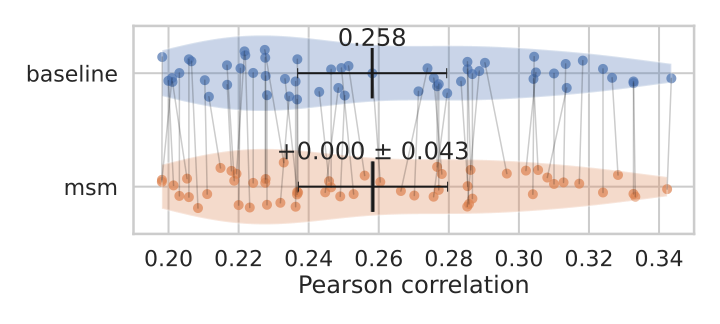
\includegraphics[width=0.49\columnwidth]{./Chapitre4/figures/fsaverage5_alignment_correlation_gain_msm.pdf}
    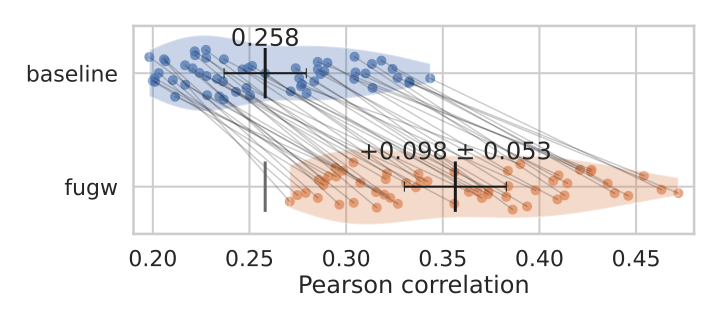
\includegraphics[width=0.49\columnwidth]{./Chapitre4/figures/fsaverage5_alignment_correlation_gain_fugw.pdf}
    \caption[Comparison of gains in correlation after inter-subject alignment]{
        \textbf{Comparison of gains in correlation after inter-subject alignment}
        For each pair of source and target subjects of the dataset,
        we compute the average Pearson correlation between 30 test contrasts,
        leading to the (baseline) correspondence score,
        and compare it with that of the same contrast maps
        aligned with either MSM (left) or FUGW (right). Correlation gains are much better for FUGW.
    }
    \label{fig:gain_comparisions_fsaverage5}
\end{figure}
% We also varied training sets by selecting subsets of training contrasts and find that
% similar performance on the test set can be achieved regardless of the training data
% (see Supplementary \Cref{sec:control_experiments} and in particular Supplementary
% \Cref{tab:varying_training_sets}).

\paragraph{Hyper-parameters selection}
\label{par:params_selection}

Hyper-parameters used to obtain these results were chosen
after running a grid search on $\alpha$, $\varepsilon$ and $\rho$
and evaluating it on the validation dataset.
Computation took about 100 hours using 4 Tesla V100-DGXS-32GB GPUs. More precisely,
it takes about 4 minutes to compute one coupling between a source and target 10k-vertex
hemisphere on a single GPU, when the solver was set to run 10 BCD and 400 Sinkhorn iterations.
In comparison, MSM takes about the same time on Intel(R) Xeon(R) CPU E5-2698 v4 @ 2.20GHz CPUs.
Results are reported in \Cref{fig:cv_metrics} and provide multiple insights concerning FUGW.

Firstly, without anatomical constraint ($\alpha = 0$),
source vertices can be matched with target vertices
that are arbitrarily far on the cortical sheet.
Even though this can significantly increase correlation, it also
results in very high vertex displacement values (up to $100mm$).
Such couplings are not anatomically plausible.
%
Secondly, without functional information ($\alpha = 1$),
couplings recover a nearly flawless matching between source and target meshes,
so that, when $\varepsilon = 10^{-5}$
(ie when we force couplings to find single-vertex-to-single-vertex matches),
vertex displacement and spread are close to 0 and correlation is unchanged.
%
Fusing both constraints ($0 < \alpha < 1$)
yields the largest gains in correlation while allowing to compute
anatomically plausible reorganizations the cortical sheet between subjects.

The impact of $\rho$ (controlling marginal penalizations) on correlation seems modest,
with a slight tendency of increased correlation in unbalanced problems (low $\rho$).

Finally, it is worth noting that a relatively wide range of $\alpha$ and $\rho$ yield comparable gains.
The fact that FUGW performance is weakly sensitive to hyper-parameters makes it
a good off-the-shelf tool for neuroscientists who wish to derive inter-individual alignments.
However, $\varepsilon$ is of dramatic importance in computed results and should be chosen carefully.
Vertex spread is a useful metric to choose sensible values of $\varepsilon$;
for human data one might consider that it should not exceed $20mm$.

\begin{figure}[ht]
    \centering
    \includegraphics[width=1\columnwidth]{./Chapitre4/figures/cv_all_metrics_hcp_left_fugw.pdf}
    \caption[Exploring hyper-parameter space to find relevant couplings]{
        \textbf{Exploring hyper-parameter space to find relevant couplings}
        Given a transport plan aligning a source and target subject,
        we evaluate how much this coupling
        (left) improves correlation between unseen contrast maps
        of the two subjects,
        (center left) actually transports data,
        (center right) moves vertices far from their original location on the cortical surface
        and (right) spreads vertices on the cortical sheet.
        We seek plans that maximize correlation gain, while keeping spread and displacement low enough.
    }
    \label{fig:cv_metrics}
\end{figure}

\paragraph{Mass redistribution in unbalanced couplings}
Unbalanced couplings provide additional information about how functional areas might differ
in size between pairs of individuals. This is illustrated in \Cref{fig:transported_mass},
where we observe variation in size of the auditory area between a given pair of individuals.
This feature is indeed captured by the difference of mass between subjects
(although the displayed contrast was not part of the training set).
\begin{figure}[!th]
    \centering
    \includegraphics[width=1\columnwidth]{./Chapitre4/figures/transported_mass.pdf}
    \caption[Transported mass indicates areas which have to be resized between subjects]{
        \textbf{Transported mass indicates areas which have to be resized between subjects}
        (Panel A) We show a contrast map from the test set which displays areas showing
        stronger activation during auditory tasks versus equivalent visual tasks. It shows much more
        anterior activations on the target subject compared to the source subject.
        This is consistent with the observation that more mass is present in
        anterior auditory areas of the source subject than in the target subject (Panel B).
    }
    \label{fig:transported_mass}
\end{figure}

\subsection{Experiment 2 - Individual anatomies}
\begin{figure}[!ht]
    \centering
    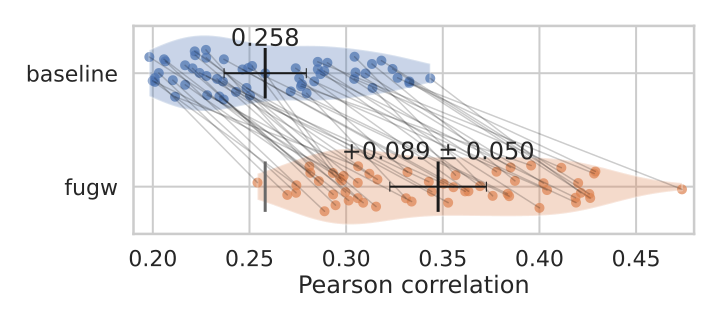
\includegraphics[width=0.5\columnwidth]{./Chapitre4/figures/individual_alignment_correlation_gain_fugw}
    \caption[Correlation between pairs of subjects is significantly better after alignment on individual anatomies than after projecting subjects onto a common anatomical template]{
        \textbf{Correlation between pairs of subjects is significantly better after alignment on individual anatomies than after projecting subjects onto a common anatomical template}
    }
    \label{fig:gain_comparisions_individual}
\end{figure}

As shown in \Cref{fig:gain_comparisions_individual},
we obtain correlation gains which are comparable to that of Experiment 1 (about 35\% gain)
while working on individual meshes.
This tends to show that FUGW can compute meaningful alignments between pairs of individuals
without the use of an anatomical template, which helps bridge most conceptual impediments listed
in \Cref{sec:introduction}.
Moreover, this opens the way for computation of simple statistics in cohorts of individuals
in the absence of a template. Indeed, one can pick an individual of the cohort and use it
as a reference subject on which to transport all other individuals.
We give an example in \Cref{fig:individual_projections},
showing that FUGW correctly preserved idiosyncrasies of each subject while
transporting their functional signal in an anatomically sound way.
\begin{figure}[H]
    \centering
    \includegraphics[width=1\columnwidth]{./Chapitre4/figures/individual_alignment.pdf}
    \caption[Transporting individual maps onto a reference subject]{
        \textbf{Transporting individual maps onto a reference subject}
        FUGW can help bridge the absence of template anatomies
        and derive pairs of alignments such that all individuals
        of the cohort are comparable. We display a map taken from the test set contrasting areas activated during mathematical reasoning against areas activated for other stimuli of the protocol.
    }
    \label{fig:individual_projections}
\end{figure}

%%%%%%%%%%%%%%%%%%%%%%%%%%%%%%%%%%%%%%%%%
\subsection{Experiment 3 - Barycenter}

In the absence of a proper metric to quantify the correctness of a barycenter,
we first qualitatively compare the functional templates obtained with and without alignment.
In \Cref{fig:barycenter_vs_group_average}.A, we do so using brain maps taken from the test set.
We can see that the barycenter obtained with FUGW yields sharper contrasts and
more fine-grained details than the barycenter obtained by per-vertex averaging.
We also display in \Cref{fig:barycenter_vs_group_average}.B
the result of a one-sample test for the same contrast, which can readily be used for inference.
The one-sample test map obtained after alignment to the FUGW template exhibits
the same supra-threshold clusters as the original approach, but also some additional spots
which were likely lost due to inter-subject variability in the \emph{fsaverage5} space.
This approach is thus very useful to increase power in group inference.
We quantify this result by counting the number of supra-threshold vertices
with and without alignment for each contrast map of the test set.
Our alignment method significantly finds more such vertices of interest,
as shown in \Cref{fig:barycenter_vs_group_average}.C.
\begin{figure}[t]
    \centering
    \includegraphics[width=1\columnwidth]{./Chapitre4/figures/barycenter_group_analysis.pdf}
    \caption[FUGW barycenter yields much finer-grained maps than group averages]{
        \textbf{FUGW barycenter yields much finer-grained maps than group averages}
        We study the same statistical map as in \Cref{fig:intro}, which contrasts
        areas of the brain involved in mathematical reasoning.
        \textbf{A}. These complex maps projected onto the barycenter and averaged
        show more specific activation patterns than simple group averages,
        especially in cortical areas exhibiting more variability, such as the prefrontal cortex.
        \textbf{B}. Deriving a t-test on aligned maps captures the same clusters
        as the classical approach (plain green circles), but also new clusters in areas
        where inter-subject variability is high (dotted black circles).
        Peak t-statistics are also higher with FUGW.
        \textbf{C}. Ratio of number of activated vertices ($|\text{t-statistic}| \geq 4$)
        with versus without alignment for each map of the test set.
        Our method finds significantly more of such vertices ($\text{p-value} = 3\cdot10^{-4}$).}
    \label{fig:barycenter_vs_group_average}
\end{figure}

\section{Discussion}

FUGW can derive meaningful couplings between pairs of subjects without
the need of a pre-existing anatomical template. It is well-suited to computing
barycenters of individuals, even for small cohorts.

In addition, we have shown clear evidence that FUGW yields gains that cannot be achieved
by traditional diffeomorphic registration methods.
These methods impose very strong constraints to the displacement field,
that may prevent reaching optimal configurations.
More deeply, this finding suggests that brain comparison ultimately requires
lifting hard regularity constraints on the alignment models,
and that two human brains differ by more than a simple continuous surface deformation.
However, current results have not shown a strong correlation gain of
unbalanced OT compared to balanced OT, likely because the cohort under study is too small.
Leveraging datasets such as HCP \citep{hcpdata} with a larger number of subjects
will help lower the standard error on correlation gain estimates.
In this work, we decided to rely on a predefined anatomical template (\emph{fsaverage5})
to derive functional barycenters.
It would be interesting to investigate whether more representative anatomical templates
can be learned during the process.
This would in particular help to customize templates to different populations or species.

Additionally, using an entropic solver introduces a new hyper-parameter $\varepsilon$
that has a strong effect, but is hard to interpret.
Future work may replace the Sinkhorn algorithm \citep{Sejourne19}
used here by the majorization-minimization one \citep{Chapel20},
which does not require entropic smoothing. This solution can yield sparse couplings
while being orders of magnitude faster, which will prove useful when computing barycenters
on large cohorts.

Finally, we plan to make use of FUGW to derive alignments between human and
non-human primates without anatomical priors. Indeed, the understanding of given brain mechanisms
will benefit from more detailed invasive measurements made on other species \emph{only if}
brains can be matched across species; moreover, this  raises the question of features
that make the human brain unique, by identifying patterns that have no counterpart in other species.
By maximizing the functional alignment between areas, but also allowing for some regions
to be massively shrunk or downright absent in one species relative to the other,
the present tool could shed an objective light on the important issue of whether
and how the language-related areas of the human cortical sheet map onto
the architecture of non-human primate brains.

\vfill

\chapter[Augmented Gromov-Wasserstein]{Augmented Gromov-Wasserstein}

\localtableofcontents*

\chaptermark{\textbf{Augmented Gromov-Wasserstein}}

\section{Introduction and motivation}

\section{Formulation and properties}

\section{Optimization and algorithm}

\section{Experiments}

\subsection{MNIST illustrations}

\subsection{Single-cell multi-omics}

\subsection{Heterogeneous domain adaptation}

\subsection{Dataset distance}

\section{Conclusion}

\chapter[Conclusion]{Conclusion}

\chaptermark{Conclusion}

\renewcommand{\contentsname}{Contents}
\localtableofcontents*
\chaptermark{\textbf{Conclusion}}

\section{Contributions}

The central motivation of this thesis is the comparison between incomparable spaces.
In particular, our work lies at the intersection of various extensions of OT,
namely the marginal relaxation, the comparison between weighted objects,
and the integration of prior knowledge. Our contributions can be organized in two main axes.

On the methodology side, we aimed to understand a few popular practices in the usage of
divergences between incomparable spaces. First, in \Cref{sec:continuous_coot},
we justify how entropic regularization can be used to approximate the GW distance and COOT.
Then in \Cref{chap:ucoot},
we show that the marginal constraints are tightly related to the impact of outliers. In particular,
relaxing them with penalization via the Kullback-Leibler divergence allows for being very robust,
whereas respecting them as in COOT and GW distance also paves the way for outliers to distort the
minimum and mislead the alignments.

On the applications side, our proposed methods address the questions arised from real-world
applications. In \Cref{chap:fugw}, we present the effectiveness of fused unbalanced GW in neuroscience,
where we showcase how it can be used to align human cortical surfaces and
learn better brain templates than the standard anatomical alignment approaches.
In computational biology, we tackle different problematics in the integration of
single-cell multi-omics data, including how to account for outliers (\Cref{chap:ucoot})
and how to better exploit the input data (\Cref{chap:agw}).
In particular, we illustrate how the proposed variations of COOT are still able to correctly recover
the relationships amongst genomic features, while providing meaningful
cell correspondences between the multi-omics datasets and even outperforming
many other OT-based competitors. These variations also show strong performance in the
heterogeneous domain adaptation tasks, especially in the unsupervised setting.

\section{Perspectives}

From the methodology perspective, we discuss some remaining follow-ups left to explore from our work.

\paragraph{An alternative solver for unbalanced OT problem}
The core engine of many unbalanced OT-based methods, notably (fused) unbalanced GW and unbalanced COOT,
relies on a solver for the unbalanced OT problem. As discussed in \Cref{sub:uot_optim},
there are few options. The \textit{de facto} Sinkhorn-based algorithms \citep{Sejourne19,Sejourne21}
usually converges slowly for small regularization, while the
Majorization-Minimization (MM) method \citep{Chapel21}
suffers the same limitation for large marginal relaxation.

One possible alternative is the inexact Bregman Proximal Point (BPP) scheme,
which is first applied to the balanced OT problem by \citet{Xie20},
known as \textit{Inexact Proximal OT} (IPOT). Interestingly,
this scheme can be easily extended to the unbalanced setting as follows.
Denote $F$ the objective function of the regularized unbalanced OT problem \eqref{eq:discrete_ent_uot}.
For fixed learning rate $\eta > 0$, at iteration $t$, we solve
\begin{align}
  \label{eq:bpp_eot}
  P^{(t+1)} \approx \argmin_{P \in \bbR^{m \times n}_{\geq 0}} F(P) + \eta \; \kl(P | P^{(t)}),
\end{align}
or equivalently,
\begin{align}
\label{eq:bpp_uot}
  P^{(t+1)} \approx \; \argmin_{P \in \bbR^{m \times n}_{\geq 0}}
  \left \langle C - \eta \log \frac{P^{(t)}}{\gamma}, P \right \rangle
  + \rho_1 \kl(P_{\# 1} | \mu) + \rho_2 \kl(P_{\# 2} | \nu) + (\varepsilon + \eta) \kl(P | \gamma).
\end{align}
The right-hand side of Equation \eqref{eq:bpp_uot} is nothing but an entropic UOT problem
with modified cost and regularization. Thus, any solvers discussed in \Cref{sub:uot_optim}
can be used. Similar to IPOT, even as few as one Sinkhorn iteration may work in practice,
meaning that the corresponding inexact solution may still empirically converge to the true minimizer
of the UOT problem.

This inexact BPP scheme has two very appealing features. First, it is flexible and versatile since
it can handle both balanced, semi-relaxed (which MM cannot), and unregularized
(which Sinkhorn-based family cannot) settings.

Second, the presence of learning rate $\eta$
increases the level of regularization in the inner entropic UOT subproblem,
thus brings two important benefits. The first one is on the reduction of number of iterations:
the larger the regularization, the faster the Sinkhorn algorithm converges. As a consequence,
running only a few iterations is usually enough to obtain a decent approximation of
the true solution. The second advantage is on the acceleration per BPP iteration. In practice,
when the regularization is not too small, one can ignore the log-domain implementation
and employ the one with direct vector-matrix multiplication,
without any concern about the numerical overflow issue.
As a result, this allows to speed up the calculation of the iterates.

However, despite the simplicity,
it appears to be difficult to study the convergence of this inexact scheme.
In particular, while it is an immediate extension of the work of \citet{Xie20} on the balanced OT,
their proof techniques of the convergence can not be adapted to the unbalanced setting.
This is because they rely on the property of the set of admissible couplings,
which is not available in the UOT. Moreover, their assumptions and conditions are also
not trivial to verify in practice, thus the convergence results are mostly of theoretical interest.

% %%%%%%%%%%%%%%%%%%%%%%%%%%%%%%%%%%%%%%%%%%%%%%
% \section{Inexact Bregman Proximal Point for Entropic Unbalanced Optimal Transport}
% \label{sec:input}

% \subsection{Motivation and algorithm}

% While usually approximated via the entropic regularization, the OT distance can also be directly
% estimated using the Bregman proximal point (BPP) method \citep{Chen93,Teboulle97}.
% Though this scheme can apply to the class of Bregman divergences,
% we will exclusively focus on the KL divergence throughout this thesis.
% More precisely, for fixed learning rate $\eta > 0$, at iteration $t$, we solve
% \begin{align}
%   \label{eq:bpp_eot}
%   P^{(t+1)} = \argmin_{P \in U(\mu, \nu)} \langle C, P \rangle + \eta \; \kl(P | P^{(t)}).
% \end{align}
% This is a slightly modified entropic OT problem and can be solved with the Sinkhorn algorithm,
% ut now the OT plan is computed by
% \begin{align}
%   P^{(t+1)} = P^{(t)} \odot \exp \left( \frac{f^{(t+1)} \oplus g^{(t+1)} - C}{\eta} \right),
% \end{align}
% where $(f^{(t+1)}, g^{(t+1)})$ is the optimal dual vectors of Problem \eqref{eq:bpp_eot}.
% Classic results \citep{Chen93} guarantee the linear convergence of BPP method
% to the minimum and the minimizer of the OT problem. Interestingly, this scheme can be easily extended to the
% generic UOT problem \eqref{eq:discrete_ent_uot}, where each iteration boils down to solving
% \begin{align}
% \label{eq:bpp_uot}
%   &P^{(t+1)} \\
%   &= \; \argmin_{P \in \bbR^{m \times n}_{\geq 0}}
%   \langle C, P \rangle + \rho_1 \kl(P_{\# 1} | \mu)
%   + \rho_2 \kl(P_{\# 2} | \nu) + \varepsilon \kl(P | \gamma) + \eta \kl(P | P^{(t)}) \\
%   &= \; \argmin_{P \in \bbR^{m \times n}_{\geq 0}}
%   \left \langle C - \eta \log \frac{P^{(t)}}{\gamma}, P \right \rangle
%   + \rho_1 \kl(P_{\# 1} | \mu) + \rho_2 \kl(P_{\# 2} | \nu) + (\varepsilon + \eta) \kl(P | \gamma).
% \end{align}
% This is nothing but an entropic UOT problem with modified cost and regularization.
% Thus, any solvers discussed in \Cref{sub:uot_optim} can be used. In particular,
% by construction, BPP is naturally applicable to the unregularized UOT.

% Interestingly, it is not necessarily to solve exactly the entropic OT problem \eqref{eq:bpp_eot},
% but even as few as one Sinkhorn iteration can work in practice.
% This approach, known as \textit{Inexact Proximal OT}, is introduced in \citep{Xie20}.
% While the inexact BPP scheme has recently been applied to the balanced OT \citep{Xie20,Yang22},
% we are not aware of any extension to the unbalanced counterpart.
% Our proposed method, called \textit{INexact Proximal Unbalanced optimal Transport} (INPUT),
% follows directly from \citep{Xie20}, since it is simple to implement and
% usually performs well in practice. The algorithmic details of INPUT can be found in \Cref{alg:isppa}.
% \begin{algorithm}[t]
%   \caption{INPUT algorithm for Problem \eqref{eq:discrete_ent_uot}.}
%   \label{alg:isppa}
% \begin{algorithmic}[1]
%   \STATE \textbf{Input:} cost matrix $C \in \bbR^{m \times n}$,
%   measures $\mu \in \bbR^m_{> 0}, \nu \in \bbR^n_{> 0}, \gamma \in \bbR^{m \times n}_{> 0}$,
%   regularization $\varepsilon \geq 0$, relaxation parameters $\rho_1, \rho_2 > 0$,
%   learning rate $\eta > 0$.
%   \FOR{$t=1, \dots, T$}
%   \STATE Calculate new cost: $C^{(t+1)} \gets C - \eta \log \Big( \frac{P^{(t)}}{\gamma} \Big)$.
%   \STATE Solve approximatively the entropic UOT problem
%   \begin{align}
%     P^{(t+1)} \approx \argmin_{P \geq 0} \; \langle C^{(t+1)}, P \rangle +
%     \rho_1 \kl(P_{\# 1} | \mu) + \rho_2 \kl(P_{\# 2} | \nu) + (\varepsilon + \eta) \kl(P | \gamma).
%   \end{align}
%   \ENDFOR
%   \STATE \textbf{Output:} transport plan $P^{(T)}$.
% \end{algorithmic}
% \end{algorithm}

% \subsection{Convergence analysis in the exact setting}

% In practice, performing the exact BPP iteration \eqref{eq:bpp_uot}
% may not be an efficient way to solve Problem \eqref{eq:discrete_ent_uot} since
% solving exactly many entropic subproblems can be computationally expensive,
% However, for theoritical interest, let us first start with the convergence analysis of this scheme.
% Thanks to Lemma 3.3 and Theorem 3.4 in \citep{Chen93}, if $P^*$ is a minimizer of
% Problem \eqref{eq:discrete_ent_uot}, then
% \begin{enumerate}
%   \item The sequence $\big( \kl(P^*, P^{(t)}) \big)_t$ is nonincreasing and converges to $0$.
%   \item The sequence $\big( F(P^{(t)}) \big)_t$ is nonincreasing and
%   \begin{align}
%     \label{eq:chen_teboulle}
%     F(P^{(t)}) - F(P^*) \leq \frac{\eta}{t} \kl(P^* | P^{(0)}).
%   \end{align}
% \end{enumerate}
% The upper bound \eqref{eq:chen_teboulle} can be further improved by exploiting the structure of
% the objective function of Problem \eqref{eq:discrete_ent_uot}.
% First, we introduce the notions of relative smoothness \citep{Bauschke17} and
% strong convexity \citep{Lu18} of a function with respect to the KL divergence.
% \begin{definition}[Bregman proximal point algorithm]
%   Given a nonepmpty closed convex set of $E \subset \bbR^d_{\geq 0}$
%   and a proper closed convex function $f: E \to \bbR$, consider the following
%   convex optimization problem
%   \begin{align}
%     \min_{x \in E} f(x).
%   \end{align}
%   For learning rate $\eta > 0$, the exact BPP scheme with respect to the KL divergence reads
%   \begin{align}
%     \label{eq:bppa}
%     x^{(t+1)} = \argmin_{x \in E} f(x) + \eta \kl(x | x^{(t)}),
%   \end{align}
%   and the inexact BPP scheme reads
%   \begin{align}
%     \label{eq:bppa_inexact}
%     x^{(t+1)} \approx \argmin_{x \in E} f(x) + \eta \kl(x | x^{(t)}).
%   \end{align}
%   Here, $x^{(t+1)}$ is only an approximate solution in some predefined sense.
% \end{definition}
% \begin{definition}
%   \label{def:smooth-convex}
%   Let $f:C \to \bbR$ be a differentiable convex function, where $C \subset \bbR^d_{\geq 0}$ is
%   a nonepmpty closed convex set. Given $L \geq 0$, we say that $f$ is $L-$smooth relative to
%   the KL divergence if for any $x, y \in C$,
%   \begin{align}
%     f(x) \leq f(y) + \langle \nabla f(y), x - y \rangle + L \; \kl(x | y).
%   \end{align}
%   Given $l \geq 0$, we say $f$ is $l-$strongly convex relative to the KL divergence
%   if for any $x, y \in C$,
%   \begin{align}
%     f(x) \geq f(y) + \langle \nabla f(y), x - y \rangle + l\; \kl(x, y).
%   \end{align}
% \end{definition}
% Recall that the objective function of Problem \eqref{eq:discrete_ent_uot} is
% $F(P) = \langle C, P \rangle + \rho_1 \kl(P_{\# 1} | \mu)
% + \rho_2 \kl(P_{\# 2} | \nu) + \varepsilon \kl(P | \gamma)$. Then, we have
% \begin{lemma}
%   \label{lemma:convex-smoothness}
%   $F$ is $\varepsilon$-strongly convex and $(\rho_1 + \rho_2 + \varepsilon)$-relatively smooth
%   with respect to the KL divergence.
% \end{lemma}
% The following result is a simple generalization of Theorem 3.1 in \citep{Lu18}.
% \begin{proposition}[Convergence rate of exact BPP for Problem \eqref{eq:discrete_ent_uot}]
%   \label{prop:convergence-exact-sppa}
%   For every $\eta > 0$, exact BPP scheme decreases the value of $F(\cdot)$ with each iteration $t$:
%   the sequence $\big( F(\pi^{(t)}) \big)_t$ is monotonically decreasing.
%   Moreover, if $\varepsilon \leq \eta \leq \rho_1 + \rho_2 + \varepsilon$,
%   then we have
%   \begin{align}
%     F(\pi^{(t)}) - F(\pi^*)
%     \leq \frac{\varepsilon}{\left( 1 +
%     \frac{\varepsilon (\rho_1 + \rho_2 + \varepsilon)}{\eta (\rho_1 + \rho_2)} \right)^t - 1}
%     \kl(\pi^* | \pi^{(0)}).
%   \end{align}
% \end{proposition}
% It is not difficult to check that this bound is weaker than the one in
% Inequality (\ref{eq:chen_teboulle}). Indeed,
% \begin{align}
%   \frac{\varepsilon}{\left( 1 +
%   \frac{\varepsilon (\rho_1 + \rho_2 + \varepsilon)}{\eta (\rho_1 + \rho_2)} \right)^t - 1}
%   \leq \frac{\varepsilon}{\frac{t \varepsilon(\rho_1 + \rho_2 + \varepsilon)}{\eta (\rho_1 + \rho_2)}}
%   = \frac{\eta}{t} \frac{\rho_1 + \rho_2}{\rho_1 + \rho_2 + \varepsilon}
%   \leq \frac{\eta}{t}.
% \end{align}

% \subsection{Convergence analysis in the inexact setting}

% Despite the simplicity, it is difficult to study the convergence of INPUT.
% In particular, while it is an immediate extension of the work of \citet{Xie20} on the balanced OT,
% their proof techniques of the convergence can not be adapted to the unbalanced setting.
% This is because they rely on the property of the set of admissible couplings,
% which is not available in the UOT. Moreover, their assumptions and conditions are also
% not trivial to verify in practice, thus the convergence results are mostly of theoretical interest.

% The convergence analysis of the inexact BPP has already been studied at the same time
% as the exact one. Typically, one can control the approximation error using
% $\varepsilon$-subdifferential \citep{Burachik97,Kiwiel97},
% or bounded subgradient \citep{Eckstein98,Rockafellar76}, to name a few.
% We are studying the literature in this domain to identify the relevant criteria, which are
% amenable to study the convergence and to verify in practice.

% \subsection{Illustration on toy example}

% \paragraph{Experimental setup}
% We consider a synthetic dataset:
% the source data $X$ contains $200$ points forming an ellipse and a square,
% assigned with the same uniform probability on both shapes
% $\mu = \frac{1}{200} \sum_{i=1}^{200} \delta_{x_i}$. The target data $Y$ also contains $200$ points
% forming an ellipse and a circle, assigned with the histogram
% $\nu = \frac{3}{200} \sum_{j=1}^{30} \delta_{y_j \in \text{Circle}} +
% \frac{7}{200} \sum_{j=31}^{100} \delta_{y_j \in \text{Circle}} +
% \frac{7}{200} \sum_{j=1}^{100} \delta_{y_j \in \text{Ellipse}}$.
% The objective in this experiment is to estimate the entropic UOT cost, where
% we choose $\gamma = \mu \otimes \nu$ and the cost $C(x, y) = || x - y||^2_2$.

% \paragraph{Competing methods}
% For INPUT, we consider $3$ versions corresponding to $3$ solvers for the inner entropic UOT problem:
% \texttt{INPUT-Sinkhorn}, \texttt{INPUT-TI-v2}, \texttt{INPUT-MM}.
% Here, we choose the variant of Sinkhorn-TI (\Cref{alg:TI_Sinkhorn_variant})
% since it is more simple to implement, yet appears to perform comparably to the Sinkhorn-TI.
% The Sinkhorn-based methods include
% \texttt{Sinkhorn} (\Cref{alg:Sinkhorn_algo}), \texttt{Sinkhorn-TI-v1} (\Cref{alg:TI_Sinkhorn})
% and its variant \texttt{Sinkhorn-TI-v2} (\Cref{alg:TI_Sinkhorn_variant}).
% We emphasize that all Sinkhorn-based methods require log-domain implementation
% for numerical stability, whereas INPUT does not suffer this issue,
% thus is implemented with direct vector-matrix multiplication.
% Apart from these $2$ families of solvers, we also evaluate the performance of
% Majorization-Minimization algorithm \texttt{MM}.

% \paragraph{Results}
% We set up $4$ scenarios to verify if INPUT can overcome the limitations of other existing methods.
% More precisely, the first one considers the situation of small relaxations and large regularization.
% It is an easy test and we expect that all methods perform well.
% In the second one, we fix the relaxations but choose small regularization
% in order to hinder convergence of Sinkhorn-based methods.
% The third scenario uses fixed regularization but very large marginal relaxations to slow down
% the convergence of MM.
% The last one combines small regularization and very large relaxations. It is designed to challenge
% both Sinkhorn and MM methods.

% It is clear that the INPUT family consistently and significantly outperforms other solvers,
% The distinction becomes even more visible in the regimes where Sinkhorn and MM struggle.
% Except for the first scenario, by contrast to its competitors,
% it seems that INPUT does not require compensating the running time for the quality of the estimation.
% We also observe that, within the family of INPUT,
% combining INPUT with Sinkhorn-TI yields the most efficient algorithm.
% Amongst the Sinkhorn-based solvers, Sinkhorn-TI shows clear improvement over Sinkhorn,
% even though this advantage quickly diminishes when regularization is small.

% \begin{table}[]
%   \small
%   \centering
%   \begin{tabular}{|cc|c|c|c|c|}
%   \hline
%   \multicolumn{2}{|c|}{} &
%     \textbf{\begin{tabular}[c]{@{}c@{}}Scenario 1\\ $\rho_1 = 40$\\ $\rho_2 = 50$\\ $\varepsilon = 1$\end{tabular}} &
%     \textbf{\begin{tabular}[c]{@{}c@{}}Scenario 2\\ $\rho_1 = 40$\\ $\rho_2 = 50$\\ $\varepsilon = 1e-3$\end{tabular}} &
%     \textbf{\begin{tabular}[c]{@{}c@{}}Scenario 3\\ $\rho_1 = 4000$\\ $\rho_2 = 5000$\\ $\varepsilon = 1$\end{tabular}} &
%     \textbf{\begin{tabular}[c]{@{}c@{}}Scenario 4\\ $\rho_1 = 4000$\\ $\rho_2 = 5000$\\ $\varepsilon = 1e-3$\end{tabular}} \\ \hline
%   \multicolumn{1}{|c|}{\multirow{3}{*}{\textbf{\begin{tabular}[c]{@{}c@{}}Sinkhorn\\ family\end{tabular}}}} &
%     \textbf{Sinkhorn} &
%     \begin{tabular}[c]{@{}c@{}}0.275 $\pm$ 0.011\\ {\color{blue}{{41.618}}} \end{tabular} &
%     \begin{tabular}[c]{@{}c@{}}55.946 $\pm$ 5.893\\ 40.588\end{tabular} &
%     \begin{tabular}[c]{@{}c@{}}{\color{red}{{0.020 $\pm$ 0.002}}} \\ 57.667\end{tabular} &
%     \begin{tabular}[c]{@{}c@{}}No convergence at \\ this tolerance\end{tabular} \\ \cline{2-6}
%   \multicolumn{1}{|c|}{} &
%     \textbf{TI-v1} &
%     \begin{tabular}[c]{@{}c@{}}0.389 $\pm$ 0.018\\ {\color{blue}{{41.618}}}\end{tabular} &
%     \begin{tabular}[c]{@{}c@{}}37.679 $\pm$ 0.926\\ {\color{red}{{40.576}}}\end{tabular} &
%     \begin{tabular}[c]{@{}c@{}}1.118 $\pm$ 0.047\\ 57.613\end{tabular} &
%     \begin{tabular}[c]{@{}c@{}}31.088 $\pm$ 0.505\\ 56.834\end{tabular} \\ \cline{2-6}
%   \multicolumn{1}{|c|}{} &
%     \textbf{TI-v2} &
%     \begin{tabular}[c]{@{}c@{}}0.318 $\pm$ 0.013\\ {\color{blue}{{41.618}}}\end{tabular} &
%     \begin{tabular}[c]{@{}c@{}}31.679 $\pm$ 2.919\\ {\color{red}{{40.576}}}\end{tabular} &
%     \begin{tabular}[c]{@{}c@{}}0.871 $\pm$ 0.034\\ 57.613\end{tabular} &
%     \begin{tabular}[c]{@{}c@{}}24.828 $\pm$ 0.243\\ 56.834\end{tabular} \\ \hline
%   \multicolumn{1}{|c|}{\multirow{3}{*}{\textbf{\begin{tabular}[c]{@{}c@{}}INPUT\\ family\end{tabular}}}} &
%     \textbf{Sinkhorn} &
%     \begin{tabular}[c]{@{}c@{}}0.190 $\pm$ 0.008\\ {\color{blue}{{41.618}}}\end{tabular} &
%     \begin{tabular}[c]{@{}c@{}}0.676 $\pm$ 0.032\\ {\color{blue}{{40.521}}}\end{tabular} &
%     \begin{tabular}[c]{@{}c@{}}1.143 $\pm$ 0.048\\ {\color{blue}{{57.608}}}\end{tabular} &
%     \begin{tabular}[c]{@{}c@{}}1.387 $\pm$ 0.026\\ {\color{blue}{{55.866}}}\end{tabular} \\ \cline{2-6}
%   \multicolumn{1}{|c|}{} &
%     \textbf{TI-v2} &
%     \begin{tabular}[c]{@{}c@{}}{\color{red}{{0.149 $\pm$ 0.008}}}\\ {\color{blue}{{41.618}}} \end{tabular} &
%     \begin{tabular}[c]{@{}c@{}}{\color{red}{{0.649 $\pm$ 0.013}}}\\ {\color{blue}{{40.521}}} \end{tabular} &
%     \begin{tabular}[c]{@{}c@{}}{\color{blue}{{0.018 $\pm$ 0.002}}} \\ {\color{red}{{57.609}}}\end{tabular} &
%     \begin{tabular}[c]{@{}c@{}}{\color{blue}{{0.079 $\pm$ 0.010}}} \\ {\color{red}{{55.868}}}\end{tabular} \\ \cline{2-6}
%   \multicolumn{1}{|c|}{} &
%     \textbf{MM} &
%     \begin{tabular}[c]{@{}c@{}} {\color{blue}{{0.068 $\pm$ 0.006}}} \\ 41.627\end{tabular} &
%     \begin{tabular}[c]{@{}c@{}} {\color{blue}{{0.186 $\pm$ 0.007}}} \\ 40.640\end{tabular} &
%     \begin{tabular}[c]{@{}c@{}}1.038 $\pm$ 0.026\\ 57.738\end{tabular} &
%     \begin{tabular}[c]{@{}c@{}}1.028 $\pm$ 0.021\\ 56.723\end{tabular} \\ \hline
%   \multicolumn{2}{|c|}{\textbf{MM}} &
%     \begin{tabular}[c]{@{}c@{}}0.193 $\pm$ 0.010\\ {\color{red}{{41.621}}} \end{tabular} &
%     \begin{tabular}[c]{@{}c@{}}0.864 $\pm$ 0.024\\ 40.558\end{tabular} &
%     \begin{tabular}[c]{@{}c@{}}0.726 $\pm$ 0.046\\ 59.089\end{tabular} &
%     \begin{tabular}[c]{@{}c@{}}{\color{red}{{0.944 $\pm$ 0.026}}} \\ 57.829\end{tabular} \\ \hline
%   \end{tabular}
%   \caption{Time $\pm$ standard deviation (in seconds) required to reach the predefined tolerance
%   (first line) and entropic UOT cost (second line). The lower score the better.
%   {\color{blue}{{Blue number}}} indicates the best score.
%   {\color{red}{{Red number}}} indicates the second best score.
%   \label{t:uot_time_compare}}
% \end{table}

% \subsection{Discussion}

% While this experiment is mainly for the proof-of-concept purpose,
% it shows that INPUT is a promising alternative solver for the UOT problem.

% \paragraph{Strengths of INPUT}
% There are two very appealing features. First, INPUT overcomes the limitations of
% the MM and Sinkhorn-based algorithms. In particular,
% it can, not only handle both balanced/unbalanced, and unregularized/regularized settings,
% but also, empirically, can converge very fast to the optimal plan and the global minimum,
% even in the regimes of very small regularization (where Sinkhorn-based methods struggles),
% or of very large relaxation (where MM converges slowly).
% We summarize the applicability of these algorithms in \Cref{t:uot_algo_compare}.

% Second, the presence of learning rate $\eta$
% increases the level of regularization in the inner entropic UOT subproblem,
% thus brings two important benefits. The first one is on the reduction of number of iterations:
% the larger the regularization, the faster the Sinkhorn algorithm converges. As a consequence,
% running only a few iterations is usually enough to obtain a decent approximation of
% the true solution. The second advantage is on the acceleration per BPP iteration. In practice,
% when the regularization is not too small, one can ignore the log-domain implementation
% and employ the one with direct vector-matrix multiplication,
% without any concern about the numerical overflow issue.
% As a result, this allows to speed up the calculation of the iterates.

% \paragraph{Weaknesses of INPUT} There is no free lunch. INPUT has two drawbacks.
% First, the cost matrix must be recalculated at the beginning of each BPP iteration.
% This can be computationally expensive and prevents INPUT from being scalable.
% Second, while tuning the learning rate is neither too tricky nor difficult,
% it may take some effort to find an appropriate value. One possible workaround,
% which usually works well in practice, is to start with $\eta$ small and not too far from $\varepsilon$.
% The intuition of this heuristic comes from \Cref{prop:convergence-exact-sppa} of exact BPP scheme,
% which indicates that, for fixed initialization, the smaller the learning rate, the smaller
% the potential gap between the estimation and the minimum.
% \begin{table}[t]
% 	\centering
% 		\begin{tabular}{|l|c|c|c|c|}
%     \hline
%     & \textbf{\makecell{Scaling}}
%     & \textbf{\makecell{TI-Sinkhorn}} & \textbf{MM} & \textbf{INPUT} \\
%     \hline
%     \makecell[l]{Unregularized \\ setting} & \nomark & \nomark & \yesmark & \yesmark \\
%     \hline
%     \makecell[l]{Balanced \\ setting} & \yesmark & \yesmark & \nomark  & \yesmark  \\
%     \hline
%     \makecell[l]{Semi-relaxed \\ setting} & \yesmark & \yesmark & \nomark  & \yesmark  \\
%     \hline
%     \makecell[l]{Major \\ drawbacks} & \makecell{Very slow conv. \\ for small $\varepsilon$}
%     & \makecell{Slow conv. \\ for small $\varepsilon$}
%     & \makecell{Slow conv. \\ for large $\rho$}
%     & \makecell{Cost recalculation, \\
%     extra tuning of \\ hyperparameters} \\
%     \hline
% 		\end{tabular}
% 		\caption{Summary of features of algorithms for entropic UOT problem \eqref{eq:discrete_ent_uot}.
%     Unregularized setting refers to $\varepsilon = 0$, balanced setting corresponds to
%     $\rho_1 = \rho_2 = \infty$ and semi-relaxed setting refers to either $\rho_1 = \infty$
%     or $\rho_2 = \infty$.
%     \label{t:uot_algo_compare}}
% \end{table}

% \paragraph{Can we adapt INPUT to solve the squared $l_2$-regularized Problem \eqref{uot_l2} ?}
% In theory, yes, since the squared $l_2$-norm is a Bregman divergence,
% thus the (inexact) BPP scheme is applicable. However, comparing to the MM solver,
% we doubt that it would bring any gain in convergence speed. Indeed,
% recall that the main motivation of INPUT comes from the poor convergence behavior of Sinkhorn
% algorithm when \textbf{regularization} is small. For this reason, adding more regularization
% to each BPP iteration helps accelerating the calculation
% and improving the convergence of the algorithm. By contrast,
% the case of squared $l_2$-norm does not suffer the same issue,
% but rather on the \textbf{relaxation} parameters. So, more regularization does not help.

\paragraph{Perspectives on GW distance} One potential application of MMOT-DC introduced
in \Cref{subsec:MMOT_DC} is on the study of the sample complexity of GW distance.
More precisely, given two measure networks $\cX = (X, c_X, \mu_X)$ and $\cY = (Y, c_Y, \mu_Y)$,
we want to quantify the convergence rate of $|\gw(\cX, \cY) - \gw(\cX_n, \cY_n)|$.
Note that, \cite{Zhang23} have also established the convergence rate for the case of $2$-GW distance,
in which the similarity is measured by squared Euclidean distance.
The advantage of the approach via MMOT-DC, would be able to handle any
conditionally negative semi-definite kernel.

The idea is as follows: under the assumptions of \Cref{prop:coot_gw_equiv},
COOT and GW distance are equivalent
\footnote{Note that one needs to properly extend \Cref{prop:coot_gw_equiv} to the continuous setting
(of measure networks).}. So, we can replace GW distance by COOT.
Next, we extend MMOT-DC to the continuous setting. In the same spirit as \Cref{interpolation_prop},
we expect that the interpolation property still holds,
notably MMOT-DC converges to COOT as regularization tends to the infinity.
Thanks to the Difference-of-Convex algorithm discussed in \Cref{sec:algo},
we can linearize the MMOT-DC and obtain an entropic MMOT problem, which has two advantages.
First, the technique used to study the sample complexity of entropic OT in \citep{Genevay19}
can be extended to the multi-marginal setting. Second, this entropic problem can approximate COOT.
Overall, the sample complexity of GW distance roughly boils down to that of an entropic MMOT problem.

% \paragraph{Perspectives on Augmented Gromov-Wasserstein (AGW)}
% While AGW has shown favorable performance over many other OT-based divergences,
% its isometries are still far from being fully understood. In particular, while
% we are able to explore the structure of \textbf{some} isometries via the singular-value
% decomposition, there are still some open questions.
% \begin{enumerate}
%     \item What is the intuition behinds the isometries induced by AGW?
%     To what extent are they "better" than those of GW distance?
%     \item Our analysis is only restricted to the case where $n \geq d$, meaning that
%     the high-dimensional setting remains staying in the dark.
%     \item We can only establish the necessary conditions. But are they also sufficient?
%     \item Given the discrete nature of AGW, it is natural the consider the continuous extension.
%     In this case, what are the characteristics of its isometries?
% \end{enumerate}

In conclusion, we hope that this thesis contributes to the theory and practice of optimal transport for
incomparable spaces, and that it will invite more applications of optimal transport in the interdisciplinary domains,
including but not limited to computational biology and neuroscience.

\vfill

\chapter*{Conclusion}

\addcontentsline{toc}{chapter}{Conclusion}

\chaptermark{Conclusion}

Hello world

% \ifenvsetTF{COMPILE_ALL}{
% 	% Compile the chapter when the COMPILE_ALL environment variable is set
% 	
\chapter[Contribution to CO-Optimal Transport]{Contribution to CO-Optimal Transport}

\localtableofcontents*

\chaptermark{\textbf{Contribution to CO-Optimal Transport}}

\section{Introduction}

This chapter is based on the paper \citep{Tran21} and my personal work.


considers a relaxation of the
CO-Optimal Transport problem. OT theory underlies many emerging machine learning
methods nowadays solving a wide range of tasks.
These latter works, however, usually build upon a traditional OT setup with two distributions,
while leaving a more general multi-marginal OT formulation somewhat
unexplored. In this paper, we study the multi-marginal OT (MMOT) problem and unify several
popular OT methods under its umbrella
by promoting structural information on the coupling. We show that incorporating such structural
information into MMOT results in an instance of a difference of convex (DC) programming problem allowing us to solve it numerically.
Despite high computational cost of the latter procedure, the solutions provided by DC optimization are usually as qualitative as
those obtained using currently employed optimization schemes.

Recall that, when the supports of the probability measures lie in the same ground metric space,
it is natural to use the distance defined by the metric
to induce the cost, which leads to the famous Wasserstein distance \citep{Villani03}.
When they do not, one can rely on the idea of Gromov-Hausdorff distance \citep{Gromov81}
and its equivalent reformulations \citep{Gromov99,Kalton99,Burago01},
and adapt them to the setting of metric measure spaces \citep{Gromov99}.
This results in, for example, the celebrated Gromov-Wasserstein distance
\citep{Memoli07,Memoli11,Sturm12}. By construction, the GW distance can only provide
the sample alignment that best preserves the intrinsic geometry of the distributions and,
as such, compares square pairwise relationship matrices.

The CO-Optimal transport (COOT) \citep{Redko20,Chowdhury21b} goes beyond these limits by
simultaneously learning two independent (feature and sample) correspondences,
thus provides greater flexibility over the GW distance in terms of usage and interpretability.
First, it allows to measure similarity between arbitrary-size matrices. An interesting use case is,
for instance, on tabular data, which is usually expressed as a matrix whose rows represent samples
and columns represent features. For the GW distance, the similarity or distance matrix
(or any square matrix derived from the data) must be calculated in advance and
the effect of the individual variables is lost during this computation. By contrast,
COOT can bypass this step as it can use either the tabular data directly or
the similarity matrices as inputs. Second, COOT provides both sample and feature correspondences.
These feature alignments are unique to COOT and prove to be particularly useful,
for example in single-cell multi-omics \citep{Demetci20b}
are also interpretable and allow to recover relations between the features of
two different datasets even when they do not lie in the same space.
COOT has shown superior performance in heterogeneous domain adaptaion \citep{Redko20},

Given a matrix $X \in \bbR^{n \times d}$,
we equip its samples (rows) with the histogram $\mu^s \in \Delta_n$ and features (columns)
with the histogram $\mu^f \in \Delta_d$.
We call the triplet $\bbX = (X, \mu^s, \mu^f)$ a sample-feature (s.f.) space.
For $p \geq 1$, we define the COOT distance between two s.f. spaces
$\bbX = (X, \mu_x^s, \mu_x^f)$ and $\bbY = (Y, \mu_y^s, \mu_y^f)$ as
\begin{align*}
    \coot(\bbX, \bbY) :=
    \inf_{\substack{\pi^s \in U(\mu_x^s, \mu_y^s) \\ \pi^f \in U(\mu_x^f, \mu_y^f)}}
    \sum_{i,j,k,l} (X_{ij} - Y_{kl})^p \pi^s_{ik} \pi^f_{jl}
    = \langle |X - Y|^p, \pi^s \otimes \pi^f \rangle.
\end{align*}
Here, for convenience, we write $|X - Y|^p$ the $4$-D tensor defined by
$(|X - Y|^p)_{i,k,j,l} = (X_{ij} - Y_{kl})^p$. We summarize the versatility of COOT for practical
usage in \Cref{t:comparisons}
\begin{table}[h]
	\centering
		\begin{tabular}{|l|l|}
    \hline
    Distance & Input matrices \\
    \hline
    Frobenius & Same-size matrices \\
    Wasserstein & Matrices with the same number of features (columns) \\
    GW & Square (mostly symmetric) matrices \\
    COOT & Arbitrary-size matrices \\
    \hline
		\end{tabular}
		\caption{but also robust to outliers.
    \label{t:comparisons}}
\end{table}
In the following sections, we will explore some aspects of COOT.

%%%%%%%%%%%%%%%%%%%%%%%%%%%%%%%%%%%%%%
\section{Three shades of discrete Co-Optimal Transport}
%%%%%%%%%%%%%%%%%%%%%%%%%%%%%%%%%%%%%%

\subsection{Co-Optimal Transport as lower bound of GW distance} \label{subsec:GWLB}

Since COOT is applicable to matrices of arbitrary-size, it is readily applicable to the GW setting,
where inputs are similarity matrices. In this case, since there is no difference between
the feature and sample distributions, we simply write $\bbX = (C^x, \mu_x)$,
where $C^x$ is the similarity matrix and $\mu_x$ is the sample distribution.
Note that GW distance can be formulated as
\begin{align}
  \gw(\bbX, \bbY) =
  \inf_{\substack{\pi, \gamma \in U(\mu_x, \mu_y) \\ \pi = \gamma }}
  \sum_{i,j,k,l} (C^x_{ij} - C^y_{kl})^p \pi_{ik} \gamma_{jl},
\end{align}
meaning that we optimize with respect to two independent couplings
under the additional constraint that they must be equal. If it is relaxed, then
one recovers the COOT distance. We also stress that it should not
be confused with the third lower bound of the GW distance \citep{Memoli07,Memoli11} defined as
\begin{equation}
  \text{TLB}(\bbX, \bbY) :=
  \inf_{\gamma \in U(\mu_x, \mu_y)}
  \Big( \inf_{\pi \in U(\mu_x, \mu_y)} \sum_{i,j,k,l} (C^x_{ij} - C^y_{kl})^p \pi_{ik}
  \Big) \gamma_{jl}
\end{equation}
In particular, it is not difficult to see that
\begin{equation}
  \label{gw_tlb_COOT}
  \gw(\bbX, \bbY) \geq \coot(\bbX, \bbY)
  \geq \text{TLB}(\bbX, \bbY).
\end{equation}
This formulation is intimately related to the \textit{bilinear assignment problem}.
The equivalence between BAP and QAP has been studied in \citep{Konno76}.
In case of the Euclidean and squared Euclidean distances, equality holds between
COOT and GW distances \citep{Sejourne20,Redko20}. Before summarizing these results,
let us recall that.
\begin{definition}
  [Conditionally positive matrix] A square matrix $A \in \bbR^{n \times n}$ is
  conditionally positive (or negative) semi-definite
  if it is symmetric and for any $c \in \bbR^n$ such that $\sum_i c_i = 0$, we have
  $c^T A c \geq 0$ (or $c^T A c \leq 0$).
\end{definition}
%%%%%%%%%%%%%%%%%%%%%%%%%%%%%%%%%%%%%%%%%%%%%%%%%%%%%%%%
\begin{proposition}
  \label{prop:coot_gw_equiv}
  For $p=2$, suppose that $C^x$ and $C^y$ are of the forms:
  $C^x_{ij} = f_i + f_j + A_{ij}$ and $C^y_{kl} = g_k + g_l + B_{kl}$,
  where $f, g$ are vectors in $\bbR^m, \bbR^n$, respectively,
  and the matrices $A, B$ are both conditionally positive (or negative) semi-definite.
  Then $\gw(\bbX, \bbY) = \coot(\bbX, \bbY)$.
  Furthermore, if $(\pi_1^*, \pi_2^*)$ is a solution of the COOT problem, then $\pi_1^*$ and $\pi_2^*$
  are two solutions of the GW problem. In particular,
  if the semi-definiteness is replaced by the definiteness, then $\pi_1^* = \pi_2^*$.
\end{proposition}
The idea relies on \citep{Maron18}, which allows to exploit the structure of the cost tensor.
One can rewrite the problem as
\begin{align}
  \vect{P}^T C^x \otimes C^y \vect{P}
\end{align}
\begin{proposition}
  (Theorem 1 in \citep{Maron18}) Denote
\begin{equation*}
    \text{lin(DS)} = \{X \in \bbR^{m \times n}: X 1_n = 0, X^T 1_m = 0 \}
\end{equation*}
the linear part of the affine-hull of the doubly-stochastic matrices. If the matrices $A \in \bbR^{m \times m}$ and
  $B \in \bbR^{n \times n}$ are both conditionally negative (or positive) semi-definite, then $\text{vec}(X)^T (B \otimes A) \text{vec}(X) \geq 0$, for every $X \in \text{lin(DS)}$.
\end{proposition}
\begin{proof}
    By lemma above, it's enough to show for any $X = u v^T$, where $u \in 1^{\perp}_m$
    and $v \in 1^{\perp}_n$. In this case, as
    $(U \otimes V)^T (A \otimes B) (U \otimes V) = (U^T A U) \otimes (V^T B V)$, we have
    $\text{vec}(u v^T)^T (B \otimes A) \text{vec}(u v^T) = (u^T A u) (v^T B v) \geq 0$.
\end{proof}
\Cref{prop:coot_gw_equiv} implies that, under certain conditions, removing
the equality constraint does not change the minimum,
thus the rationale behind the alternative minimization procedure of GW distance is justified.
In practice, this idea of using COOT to approximate the GW distance has been used to
solve the unbalanced GW problem \citep{Sejourne20,Thual22}. It can also be extended
easily to the setting of fused GW. To see this, first, observe that
\begin{align}
  \text{FGW}_{\alpha}(\bbX, \bbY) =
  \inf_{\substack{\pi, \gamma \in U(\mu_x, \mu_y) \\ \pi = \gamma }}
  \sum_{i,j,k,l} (C^x_{ij} - C^y_{kl})^p \pi_{ik} \gamma_{jl} +
  \frac{\alpha}{2} \langle D, \pi \rangle + \frac{\alpha}{2} \langle D, \gamma \rangle.
\end{align}
Under exactly the same conditions, one can drop the equality constraint during the optimization.
This result justifies the use of Block Coordinate Descent to estimate the FGW distance.

%%%%%%%%%%%%%%%%%%%%%%%%%%%%%%%%
\subsection{Co-Optimal Transport as low non-negative rank OT}

Recently, low non-negative rank OT \citep{Meyer21a} and extended to the GW and unbalanced settings
\citep{Meyer21b,Meyer23}. The idea is based on the \citep{Joel93} and first applied to OT by
\citep{Forrow18}, then more complete analysis in \citep{Meyer22}.
\begin{definition}
  [\citep{Joel93}]
  Given a non-negative matrix $A$, we define its non-negative rank by
  \begin{equation*}
    \rank_{+}(A):= \min \big\{ r \geq 1: A = \sum_{i=1}^r M_i,
    \text{ where } \rank(M_i) = 1, M_i \geq 0, \forall i \big\}.
  \end{equation*}
  By convention, zero matrix has zero (thus non-negative) rank.
\end{definition}
To estimate how large can the non-negative rank be, Lemma 2.3 in \citep{Joel93} states that
$\rank(A) \leq \rank_+(A) \leq \min(m, n)$, for any nonnegative matrix $A \in \bbR^{m \times n}$.
Now, the low non-negative rank OT (LROT) is defined as
\begin{align*}
  \min_{P \in U(\mu, \nu)} &\langle C, P \rangle \\
  \text{ s.t. } &\rank_+(P) \leq r.
\end{align*}
Now, we will show that COOT is in fact as a variation of the LROT.
First, let us define three following reshaping operations.
\begin{itemize}
  \item[$\bullet$] Vectorization: concatenates rows of a matrix into a vector.
  \begin{equation*}
    \vect: \bbR^{m \times n} \to \bbR^{m n},
  \end{equation*}
  where each element $A_{i,j}$ of the matrix $A \in \bbR^{m \times n}$ is
  mapped to a unique element $b_{(i-1)n + j}$ of the vector
  $b \in \bbR^{m n}$, with $A_{i,j} = b_{(i-1)n + j}$, for $i = 1, ..., m$ and $j = 1, ...,n$.
  Conversely, each element $b_k$ is mapped to a unique element $A_{k // n, n - k \% n}$,
  for every $k = 1, ..., mn$. Here, $k // n$ and $k \% n$ are the quotient and
  the remainder of the division of $k$ by $n$,
  respectively, i.e. if $k = q n + r$, with $0 \leq r < n$, then $k // n = q$ and $k \% n = r$.

  \item[$\bullet$] Matrization: transforms a $4$D tensor to a $2$D tensor (matrix) by
  vectorizing the first two and the last two dimensions of the tensor.
  \begin{equation*}
    \text{mat}: \bbR^{n_1 \times n_2 \times n_3 \times n_4} \to \bbR^{(n_1 n_2) \times (n_3 n_4)},
  \end{equation*}
  where, similar to the vectorization, each element $P_{i,j,k,l}$ of the tensor
  $P \in \bbR^{n_1 \times n_2 \times n_3 \times n_4}$ is mapped to
  a unique element $A_{(i-1)n_2 + j, (k-1)n_4 + l}$ of the
  matrix $A \in \bbR^{(n_1 n_2) \times (n_3 n_4)}$,
  with $P_{i,j,k,l} = A_{(i-1)n_2 + j, (k-1)n_4 + l}$.

  \item[$\bullet$] Concatenation: stacks vertically two equal-column matrices.
  \begin{equation*}
    \begin{split}
      \text{con}_v: &\bbR^{m \times d} \times \bbR^{n \times d} \to \bbR^{(m+n) \times d} \\
      & \big( (u_1, ..., u_m),(v_1, ..., v_n) \big) \to (u_1, ..., u_m, v_1, ..., v_n)^T.
    \end{split}
  \end{equation*}
  Or, stacks horizontally two equal-row matrices
  \begin{equation*}
    \begin{split}
      \text{con}_h: &\bbR^{n \times p} \times \bbR^{n \times q} \to \bbR^{n \times (p+q)} \\
      & \big( (u_1, ..., u_p),(v_1, ..., v_q) \big) \to (u_1, ..., u_p, v_1, ..., v_q).
    \end{split}
  \end{equation*}
\end{itemize}
\begin{lemma} \label{vec_mat}
  For any $4$-D tensor $P \in \bbR^{n_1 \times n_2 \times n_3 \times n_4}$,
  denote $\pi$ its matrization. We have,
  \begin{equation*}
    \vect \Big( \sum_{k,l} P_{\cdot, \cdot, k, l} \Big) = \sum_{n=1}^{n_3 n_4} \pi_{\cdot, n} = \pi 1_{n_3 n_4},
  \end{equation*}
  where $1_n$ is the vector of ones in $\bbR^n$.
\end{lemma}
\begin{proof}
For $(i,j) \in [n_1] \times [n_2]$, we have
\begin{align*}
    \vect \Big(\sum_{k,l} P_{\cdot,\cdot, k, l}\Big)_{(i-1)n_2 + j} &= \sum_{k,l} P_{i,j,k,l} \\
    &= \sum_{k,l} \pi_{(i-1) n_2 + j, (k-1) n_4 + l} \\
    &= \sum_{n=1}^{n_3 n_4} \pi_{(i-1) n_2 + j, n}.
\end{align*}
The result then follows.
\end{proof}
Now, let $(e_i)_{i=1}^{n_1 n_2}$ be the standard basis vectors of $\bbR^{(n_1 n_2)}$,
\ie $(e_i)_k = 1_{\{i=k\}}$. For each $P \in U(\mu)$, denote $\pi$ its matrisation,
then by \Cref{vec_mat}, we have, for $i \in [n_1]$,
\begin{equation*}
  (\mu_1)_i = \sum_j \sum_{k,l} P_{i,j,k,l} = \sum_{j = 1}^{n_2} \sum_{n=1}^{n_3 n_4} \pi_{(i-1) n_2 + j, n},
\end{equation*}
which can be recast in matrix form as $A_1^T \pi 1_{n_3 n_4} = \mu_1$,
where the matrix $A_1 = \text{con}_{h}(v_1, ..., v_{n_1}) \in \bbR^{(n_1 n_2) \times n_1}$,
with $v_i \in \bbR^{(n_1 n_2)}$, where $v_i = \sum_{j=(i-1)n_2 + 1}^{i n_2} e_j$,
with $i \in [n_1]$. Similarly, $A_2 \pi 1_{n_3 n_4} = \mu_2$, where the matrix
$A_2 = \text{con}_h(I_{n_2}, ..., I_{n_2}) \in \bbR^{n_2 \times (n_1 n_2)}$,
where $I_n \in \bbR^{n \times n}$ is the identity matrix.
Both conditions can be compactly written as $A_{12}^T \pi 1_{n_3 n_4} = \mu_{12}$,
where the matrix $A_{12} = \text{con}_h(A_1, A_2^T) \in \bbR^{(n_1 n_2) \times (n_1+n_2)}$ and
$\mu_{12} = \text{con}_v(\mu_1, \mu_2) \in \bbR^{(n_1 + n_2)}$.
Note that $\mu_{12}$ is not a probability because its mass is $2$.
The matrix $A_{12}$ has exactly $2n_1n_2$ ones and the rest are zeros.
An example of $A_{12}$ is shown in \Cref{fig:matrix_a12}.

Similarly, for $A_{34}$ and $\mu_{34}$ defined in the same way as $A_{12}$ and
$\mu_{12}$, respectively, we establish the equality $A_{34}^T \pi^T 1_{n_1 n_2} = \mu_{34}$.
As a side remark, both matrices $A_{12}^T$ and $A_{34}^T$ are \textit{totally unimodular},
meaning that every square submatrix has determinant $-1, 0$, or $1$.
\begin{figure}[h]
  \centering
  \includegraphics[height=0.25\textheight,keepaspectratio]{./Chapitre2/fig/matrix.pdf}
  \caption{An example of the matrix $A_{12}$ when $n_1=2$ and $n_2=3$.}
  \label{fig:matrix_a12}
\end{figure}

We also have that, the condition $P = P_1 \otimes P_2$ can be rewritten as
$\text{mat}(P) = \vect(P_1) \vect(P_2)^T$. By Lemma 2.1 in \citep{Joel93}, $\text{rank}_+(A) = 1$
if and only if there exist two non-negative vectors $u,v$ such that
$A = u v^T$. Thus, the factorization constraint is equivalent to
$\text{rank}_+\big( \text{mat}(P) \big) = 1$.

Now, denote $L= \text{mat}(C)$ and $M = n_1 n_2, N = n_3 n_4$. COOT can be rewritten as
\begin{equation*}
  \begin{split}
    \min_{Q \in \bbR^{M \times N}_{\geq 0}} &\langle L, Q \rangle \\
    \text{ such that } & A_{12}^T Q 1_N = \mu_{12} \\
    &A_{34}^T Q^T 1_M = \mu_{34} \\
    &\text{rank}_{+}(Q) = 1,
  \end{split}
\end{equation*}
which is a variation of the non-negative rank-$1$ OT problem.

%%%%%%%%%%%%%%%%%%%%%%%%%%%%%%%%%%%%%%
\subsection{Co-Optimal Transport as factored multi-marginal OT} \label{subsec:MMOT_DC}

Note that we can rewrite COOT as a variation of multi-marginal OT (MMOT) problem.
To see this, first, we recall some related concepts.
Given an integer $N \geq 1$, for any positive integers $a_1,..., a_N$, we call
$P \in \bbR^{a_1 \times ... \times a_N}$ a $N$-D tensor. In particular,
a $1$-D tensor is a vector and $2$-D tensor is a matrix.
A tensor is a probability tensor if its entries are non-negative and the sum of all entries is $1$.
Given $N$ probability vectors $\mu_1, ..., \mu_N$, we write $\mu = (\mu_n)_{n=1}^N$.
We denote $\Sigma$ the set of $N$-D probability tensors and $U(\mu) \subset \Sigma$ the set of non-negative tensors whose $N$
marginal distributions are $\mu_1, ..., \mu_N$. In this case, any coupling in $U(\mu)$ is said to be \textit{admissible}.

Given a collection of $N$ histograms $\mu = (\mu_n \in \bbR^{a_n})_{n=1}^N$
and a $N$-D cost tensor $C \in \bbR^{a_1 \times ... \times a_N}$, the MMOT problem reads
\begin{equation*}
  \text{MMOT}(\mu) = \inf_{P \in U(\mu)} \langle C, P \rangle.
\end{equation*}
In practice, such a formulation is intractable to optimize in a discrete setting as it results in a linear program where the number
of constraints grows exponentially in $N$. A more tractable strategy for solving MMOT is to consider the following entropic
regularization problem
\begin{equation} \label{MMOT_primal}
  \inf_{P \in U(\mu)} \langle C, P \rangle + \varepsilon H(P).
\end{equation}
which can be solved using Sinkhorn's algorithm \citep{Benamou14}. We refer the interested reader to Supplementary materials for algorithmic details.

\paragraph{Derivation of the Sinkhorn algorithm in entropic MMOT.} The corresponding entropic dual problem of the primal problem
\ref{MMOT_primal} reads
\begin{equation*}
  \sup_{f_n \in \bbR^{a_n}} \sum_{n=1}^N \langle f_n, \mu_n \rangle -
  \varepsilon \sum_{i_1,...,i_N} \exp\Big( \frac{\sum_n (f_n)_{i_n} - C_{i_1,...,i_N}}{\varepsilon} \Big) + \varepsilon.
\end{equation*}
For each $n \in [N]$ and $i_n \in [a_n]$, the first order optimality condition reads
\begin{equation*}
  0 = (\mu_n)_{i_n} - \exp\big( \frac{(f_n)_{i_n}}{\varepsilon} \big)
  \sum_{i_{-n}} \exp\Big( \frac{\sum_{j \neq n} (f_j)_{i_j} - C_{i_1,...,i_N}}{\varepsilon} \Big),
\end{equation*}
where, with some abuse of notation, we write $i_{-n} = (i_1, ..., i_{n-1}, i_{n+1}, ..., i_N)$. Or, equivalently
\begin{equation*}
  (f_n)_{i_n} = \varepsilon \log (\mu_n)_{i_n} - \varepsilon \log \sum_{i_{-n}}
  \exp\Big( \frac{\sum_{j \neq n} (f_j)_{i_j} - C_{i_1,...,i_N}}{\varepsilon} \Big),
\end{equation*}
or even more compact form
\begin{equation*}
  f_n = \varepsilon \log \mu_n - \varepsilon \log \sum_{i_{-n}}
  \exp\Big( \frac{\sum_{j \neq n} (f_j)_{i_j} - C_{\cdot, i_{-n}}}{\varepsilon} \Big).
\end{equation*}
Using the primal-dual relation, we obtain the minimiser of the primal problem \ref{MMOT_primal} by
\begin{equation*}
  P_{i_1,...,i_N} = \exp\Big( \frac{\sum_n (f_n)_{i_n} - C_{i_1,...,i_N}}{\varepsilon} \Big),
\end{equation*}
for $i_n \in [a_n]$, with $n \in [N]$.
%%%%%%%%%%%%%%%%%%%%%%%%%%%%%%%%%%%%%%%%%
Similar to the entropic OT, the Sinkhorn algorithm \ref{algo:dual_mmot} is also usually implemented in log-domain to avoid numerical instability.
\begin{algorithm}[h]
  \caption{Sinkhorn algorithm for the entropic MMOT problem \ref{MMOT_primal} from \citep{Benamou14}.}
  \textbf{Input.} Histograms $\mu_1,...,\mu_N$, hyperparameter $\varepsilon > 0$, cost tensor $C$ and
  tuple of initial dual vectors $(f^{(0)}_1, ... f^{(0)}_N)$.

  \textbf{Output.} Optimal transport plan $P$ and tuple of dual vectors $(f_1, ... f_N)$ (optional).
  \begin{enumerate}
    \item While not converge: for $n = 1, ..., N$,
    \begin{equation*}
      \begin{split}
        f^{(t+1)}_n &= \varepsilon \log \mu_n - \varepsilon \log \sum_{i_{-n}}
        \Big[ \exp\Big( \frac{\sum_{j < n} (f^{(t+1)}_j)_{i_j} + \sum_{j > n} (f^{(t)}_j)_{i_j} -
        C_{\cdot, i_{-n}}}{\varepsilon} \Big) \Big].
      \end{split}
    \end{equation*}
    \item Return tensor $P$, where for $i_n \in [a_n]$, with $n \in [N]$,
    \begin{equation*}
      P_{i_1,...,i_N} = \exp\Big( \frac{\sum_n (f_n)_{i_n} - C_{i_1,...,i_N}}{\varepsilon} \Big).
    \end{equation*}
  \end{enumerate}
  \label{algo:dual_mmot}
\end{algorithm}

Now, it is easy to see that COOT can be rewritten as
\begin{align*}
  \inf_{\gamma \in U_2} \langle C, \gamma \rangle
\end{align*}
where $U_2 = {\gamma \in U(\mu): \gamma = \pi^s }$

\paragraph{Contributions} We define and study a general MMOT problem with structural penalization on the coupling matrix.
We start by showing that a such formulation includes several popular OT methods as special cases and allows to gain deeper insights
into them. We further consider a relaxed problem where the hard constraint is replaced by a regularization term and show that it leads
to an instance of the difference of convex programming problem. A numerical study of the solutions obtained when solving the latter
in cases of interest highlights their competitive performance when compared to solutions provided by the optimization
strategies used previously.

\subsubsection*{Factored MMOT and its relaxation}
We start by giving several definitions used in the following parts of the paper.
%We call $P \in \bbR^{a_1 \times ... \times a_N}$ a $N$-D tensor. When $N=1$, we simply call it a vector and when $N=2$,
%it is a matrix.
\begin{definition}[Tuple partition]
 Given two integers $N \geq M \geq 2$, a sequence of tuples $\mathcal T = (\mathcal T_m)_{m=1}^M$, is called a
 \underline{tuple partition} of the $N$-tuple $(1,...,N)$ if the tuples $\mathcal T_1, ..., \mathcal T_M$ are nonempty and disjoint,
 and their concatenation in this order gives $(1,...,N)$.
\end{definition}
Here, we implicitly take into account the order of the tuple, which is not the case for the partition of the set $[N]$. If
there exists a tuple in $\mathcal T$ which contains only one element, then we say $\mathcal T$ is \textit{degenerate}.

\begin{definition}[Marginal tensor]
  Given a tensor $P \in \bbR^{a_1 \times ... \times a_N}$ and a tuple partition $\mathcal T = (\mathcal T_m)_{m=1}^M$,
  we call $P_{\# \mathcal T_m}$ its \underline{$\mathcal T_m$-marginal tensor}, by summing $P$ over all dimensions not in $\mathcal T_m$.
  We write $P_{\# \mathcal T} = P_{\# \mathcal T_1} \otimes ... \otimes P_{\# \mathcal T_M} \in \bbR^{a_1 \times ... \times a_N}$
  the tensor product of its marginal tensors.
\end{definition}
For example, for $M=N=2$, we have $\mathcal T_1 = (1)$ and $\mathcal T_2 = (2)$. So, given a matrix
$P \in \bbR^{a_1 \times a_2}$, its marginal tensors $P_{\# \mathcal T_1}$ and $P_{\# \mathcal T_2}$ are simply vectors in
$\bbR^{a_1}$ and $\bbR^{a_2}$, respectively, defined by $(P_{\# \mathcal T_1})_i = \sum_j P_{ij}$ and
$(P_{\# \mathcal T_2})_j = \sum_i P_{ij}$ for $(i,j) \in [a_1] \times [a_2]$. The tensor product
$P_{\# \mathcal T} \in \bbR^{a_1 \times a_2}$ is then defined by
$(P_{\#\mathcal T})_{ij} = (P_{\# \mathcal T_1})_i (P_{\# \mathcal T_2})_j$.

Clearly, if $P$ is a probability tensor, then so are its marginal tensors and tensor product.

Suppose $\mathcal T_m = (p,...,q)$ for some $m \in [M]$ and $1 \leq p \leq q \leq N$. We denote
$\Sigma_{\mathcal T_m}$ the set of probability tensors in $\bbR^{a_p \times ... \times a_q}$ and
$U_{\mathcal T_m} \subset \Sigma_{\mathcal T_m}$ the set
of probability tensors in $\bbR^{a_p \times ... \times a_q}$ whose $(r)$-marginal vector is $\mu_r$, for every $r = p,...,q$.

%%%%%%%%%%%%%%%%%%%%%%%%%%%%%%%
\begin{definition}[Factored MMOT]
  Given a collection of histograms $\mu = (\mu_n)_{n=1}^N$ and a tuple partition $\mathcal T = (\mathcal T_m)_{m=1}^M$,
  we consider the following OT problem
  \begin{equation} \label{factor_mmot}
    \text{F-MMOT}( \mathcal T, \mu) = \inf_{P \in U_{\mathcal T}} \langle C, P \rangle,
  \end{equation}
  where $U_{\mathcal T} \subset U(\mu)$ is the set of admissible couplings which can be factorized as a tensor product of $M$
  component probability tensors in $\Sigma_{\mathcal T_1}, ..., \Sigma_{\mathcal T_M}$.
\end{definition}
Several remarks are in order here. First, one should note that the partition considered above is in general not degenerate meaning
that the decomposition can involve tensors of an arbitrary order $<N$. Second, the decomposition in this setting depicts the prior
knowledge regarding the tuples of measures which should be independent: the couplings for the measures from different tuples will
be degenerate and the optimal coupling tensor will be reconstructed from couplings of each tuple separately.
Third, suppose the partition $(\mathcal T_m)_{m=1}^M$ is not degenerate and $M=2$, i.e. the tensor is factorized as product of
two tensors, the problem \cref{factor_mmot} is equivalent to a variation of low non-negative rank OT problem (see Appendix for a proof).

As for the existence of the solution to this problem, we have that $U_{\mathcal T}$ is compact because it is a close subset of the
compact set $U(\mu)$, which implies that the problem \cref{factor_mmot} always admits a solution. Furthermore, observe that
\begin{equation*}
  \begin{split}
    U_{\mathcal T} &= \{ P \in U(\mu): P = P_1 \otimes ... \otimes P_M, \text{where } P_m \in \Sigma_{\mathcal T_m}, \forall m = 1,...,M \} \\
    &= \{ P \in \Sigma: P = P_1 \otimes ... \otimes P_M, \text{where } P_m \in U_{\mathcal T_m}, \forall m = 1,...,M \}.
  \end{split}
\end{equation*}
Thus, the problem F-MMOT can be rewritten as
\begin{equation*}
  \text{F-MMOT}( \mathcal T, \mu) = \inf_{\substack{P_m \in U_{\mathcal T_m} \\ \forall m = 1,...,M}}
  \langle C, P_1 \otimes ... \otimes P_M \rangle.
\end{equation*}
So, if $\mathcal T_1,...,\mathcal T_M$ are $2$-tuples and two marginal distributions corresponding to each $U_{\mathcal T_m}$ are
identical and uniform, then by Birkhoff's theorem \citep{Birkhoff46}, the problem \ref{factor_mmot} admits an optimal solution in
which each component tensor $P_m$ is a permutation matrix.

\paragraph{Two special cases.} When $N = 4$ and $M=2$ with $\mathcal T_1 = (1,2)$ and $\mathcal T_2 = (3,4)$, the problem
\ref{factor_mmot} becomes the CO-Optimal transport (COOT), where the two component tensors are known as
\textit{sample} and \textit{feature} couplings. If furthermore, $a_1 = a_3, a_2=a_4$, and $\mu_1 = \mu_3, \mu_2=\mu_4$, it becomes a
lower bound of the discrete Gromov-Wasserstein (GW) distance \citep{Memoli11}. This means that our formulation can be seen as a
generalization of several OT formulations.

%%%%%%%%%%%%%%%%%%%%%%%%%%%%%%%%%%%%%%%%%%%%%
Observe that if a probability tensor $P$ can be factorized as a tensor product of probability tensors, i.e.
$P = P_1 \otimes ... \otimes P_M$, then each $P_m$ is also the $\mathcal T_m$-marginal tensor of $P$. In this case,
we have $P = P_{\# \mathcal T}$. This prompts us to consider the following relaxation of factored MMOT, where the hard constraint
$U_{\mathcal T}$ is replaced by a regularization term.
\begin{definition}[Relaxed Factored MMOT]
  Given $\varepsilon \geq 0$, a collection of measures $\mu$ and a tuple partition $\mathcal T$,
  we define the following problem:
  \begin{equation} \label{relax_mmot}
    \text{MMOT-DC}_{\varepsilon}( \mathcal T, \mu) =
    \inf_{P \in U(\mu)} \langle C, P \rangle + \varepsilon \kl(P \vert P_{\# \mathcal T}).
  \end{equation}
\end{definition}
From the exposition above, one can guess that this relaxation is reminiscent of the entropic regularization in MMOT and
coincides with it when $M = N$. As such, it also recovers the classical entropic OT. One should note that the choice of the KL
divergence is not arbitrary and its advantage will become clear when it comes to the algorithm. %A well known
A special case of the problem \ref{relax_mmot} is when $M = N$, we recover the entropic-regularized MMOT problem, up to a constant.

After having defined the two optimization problems, we now set on exploring their theoretical properties.

\subsubsection*{Theoretical properties}
%The following properties are direct consequences of the definition.
Intuitively, the relaxed problem is expected to allow for solutions with a lower value of the final objective function. We formally prove the validity of this intuition below.
%%%%%%%%%%%%%%%%%%%%%%%%%%%%%%%%%%%%%%%%%%%%%
\begin{proposition}[Preliminary properties] \label{MMOT_dc_prop}
  Given a collection of histograms $\mu$ and a tuple partition $\mathcal T$,
  \begin{enumerate}
    \item For every $\varepsilon \geq 0$, we have $\text{MMOT}(\mu) \leq
    \text{MMOT-DC}_{\varepsilon}(\mathcal T, \mu) \leq \text{F-MMOT}( \mathcal T, \mu)$.
    \item For every $\varepsilon > 0, \text{MMOT-DC}_{\varepsilon}( \mathcal T, \mu ) = 0$ if and only if
    $\text{F-MMOT} (\mathcal T, \mu) = 0$.
  \end{enumerate}
\end{proposition}
%%%%%%%%%%%%%%%%%%%%%%%%%%%%%%%%%%%%%%%%%%%%%
An interesting property of MMOT-DC is that it interpolates between MMOT and F-MMOT. Informally,
for very large $\varepsilon$, the KL divergence term dominates, so the optimal transport plans tend to be factorizable.
On the other hand, for very small $\varepsilon$, the KL divergence term becomes negligible and we approach MMOT.
The result below formalizes this intuition.
%%%%%%%%%%%%%%%%%%%%%%%%%%%%%%%%%%%%%%%%%%%%%
\begin{proposition}[Interpolation between MMOT and F-MMOT] \label{interpolation_prop}
  For any tuple partition $\mathcal T$ and for $\varepsilon > 0$,
  let $P_{\varepsilon}$ be a minimiser of the problem $\text{MMOT-DC}_{\varepsilon}(\mathcal T, \mu)$.
  \begin{enumerate}
    \item When $\varepsilon \to \infty$, one has $\text{MMOT-DC}_{\varepsilon}(\mathcal T, \mu) \to
    \text{F-MMOT}(\mathcal T, \mu)$. In this case, any cluster point of the sequence of minimisers
    $(P_{\varepsilon})_{\varepsilon}$ is a minimiser of $\text{F-MMOT}(\mathcal T, \mu)$.

    \item When $\varepsilon \to 0$, then $\text{MMOT-DC}_{\varepsilon}(\mathcal T, \mu) \to \text{MMOT}(\mu)$.
    In this case, any cluster point of the sequence of minimisers $(P_{\varepsilon})_{\varepsilon}$ is a minimiser of
    $\text{MMOT}(\mu)$.
  \end{enumerate}
\end{proposition}
%%%%%%%%%%%%%%%%%%%%%%%%%%%%%%%%%%%%%%%%%%%%%
\paragraph{GW distance revisited.} Somewhat surprisingly, the relaxation \ref{relax_mmot} also allows us to prove the equality
between GW distance and COOT in the discrete setting. Let $\mathcal X$ be a
finite subset (of size $m$) of a certain metric space. Denote $C_x \in \bbR^{m \times m}$ its similarity matrix (e.g. distance
matrix). We define similarly the set $\mathcal Y$ of size $n$ and the corresponding similarity matrix $C_y \in \bbR^{n \times n}$.
We also assign two discrete probability measures $\mu_x \in \bbR^m$ and $\mu_y \in \bbR^n$ to $\mathcal X$ and $\mathcal Y$,
respectively. The GW distance is then defined as
\begin{equation*}
  \gw(C_x, C_y) = \inf_{Q \in U(\mu_x, \mu_y)} \langle L(C_x, C_y), Q \otimes Q \rangle,
\end{equation*}
and the COOT reads
\begin{equation*}
  \coot(C_x, C_y) = \inf_{\substack{Q_s \in U(\mu_x, \mu_y) \\ Q_f \in U(\mu_x, \mu_y)}}
  \langle L(C_x, C_y), Q_s \otimes Q_f \rangle,
\end{equation*}
where $L(C_x,C_y) \in \bbR^{m \times n \times m \times n}$ represents the $4$-D cost tensor induced by the matrices $C_x$ and $C_y$,
and $U(\mu, \nu)$ is the set of couplings in $\bbR^{m \times n}_{\geq 0}$ whose two marginal distributions are $\mu$ and
$\nu$. When $C_x$ and $C_y$ are two squared Euclidean distance matrices, and $L(C_x,C_y)$ is of the form
$\big(L(C_x,C_y)\big)_{i,j,k,l} = \vert (C_x)_{i,k} - (C_y)_{j,l} \vert^2$, it can be shown that the GW distance is equal
to the COOT. This is also true when $L(C_x, C_y)$ is a negative definite kernel \citep{Sejourne20}.
Here, we establish a weaker case where this equality still holds.
%%%%%%%%%%%%%%%%%%%%%%%%%%%%%%%%%%%%%%%%%%%%%
\begin{corollary} \label{kernel_gw_coot}
  If $L(C_x, C_y)$ defines a conditionally negative definite kernel on $(\mathcal X \times \mathcal Y)^2$, then we have the equality
  between GW distance and COOT. Furthermore, if $(Q_s^*,Q_f^*)$ is a solution of the COOT problem, then $Q_s^*$ and $Q_f^*$ are
  two solutions of the GW problem. In particular, when $L(C_x, C_y)$ induces a strictly positive definite kernel
  $\exp \big( -\frac{L(C_x, C_y)}{\varepsilon} \big)$, for every $\varepsilon > 0$, we have $Q_s^* = Q_f^*$.
\end{corollary}
%%%%%%%%%%%%%%%%%%%%%%%%%%%%%%%%%%%%%%%%%%%%%
The proof relies on the connection between MMOT-DC and COOT shown in the \cref{interpolation_prop},
and given a
$4$-D solution of MMOT-DC, we can construct another $4$-D solutions whose
$\mathcal T_1$ and $\mathcal T_2$-marginal matrices are identical,
under the assumption of the cost tensor. The proof of the second claim is deferred to the Appendix.
Note that, this result is more general than the one in the previous section, where

\subsubsection*{Numerical solution} \label{sec:algo}
%%%%%%%%%%%%%%%%%%%%%%%%%%%%%%%%%%%%%%%%%%%%%
We now turn to the computational aspect of the problem \ref{relax_mmot}. First, note that for any tuple partition
$\mathcal T = (\mathcal T_m)_{m=1}^M$ and probability tensor $P$, the KL divergence term can be decomposed as
\begin{equation*}
  \kl(P \vert P_{\# \mathcal T}) = H(P) - \sum_{m=1}^m H_m(P),
\end{equation*}
where the function $H_m$ defined by $H_m(P) := H(P_{\# \mathcal T_m})$ is continuous and convex with respect to $P$.
Now, the problem \ref{relax_mmot} becomes
\begin{equation} \label{relax}
  \text{MMOT-DC}_{\varepsilon}(\mathcal T, \mu) = \inf_{P \in U(\mu)}
  \langle C, P \rangle + \varepsilon H(P) - \varepsilon \sum_{m=1}^M H_m(P).
\end{equation}
This is nothing but a Difference of Convex (DC) programming problem (which explains the name MMOT-DC),
thanks to the convexity of the set $U(\mu)$ and the entropy function $H$. Thus, it can be solved
by the classic DC algorithm
\footnote{The DC algorithm is very closely related to Convex-concave procedure, majorization-minimization algorithm, Successive Linear
Approximation. For a detailed discussion on the subtle distinction amongst these name, see
\citep{}} \citep{Tao86,Tao97} as follows: at the iteration $t$,
\begin{enumerate}
  \item Calculate $G^{(t)} \in \partial(\sum_{m=1}^M H_m)(P^{(t)})$.
  \item Solve $P^{(t+1)} \in \arg\min_{P \in U(\mu)} \langle C -
  \varepsilon G^{(t)}, P \rangle + \varepsilon H(P)$.
\end{enumerate}
%%%%%%%%%%%%%%%%%%%%%%%%%%%%%%%%%%%%%%%%%%%%%%
This algorithm is very easy to implement. Indeed, the second step is an entropic-regularized MMOT problem, which admits a unique
solution, thanks to the strict convexity of the objective function. Such solution can be found by the Sinkhorn algorithm
\ref{algo:dual_mmot}. In the first step, the gradient can be calculated explicitly.
For the sake of simplicity, we illustrate the calculation in a simple case, where $M=2$ and $N=4$ with
$\mathcal T_1$ and $\mathcal T_2$ are two $2$-tuples. The function $H_1 + H_2$ is continuous, so
$G^{(t)} = \nabla_P (H_1 + H_2)(P^{(t)})$. Given a $4$-D probability tensor $P$, we have
\begin{equation*}
  H_1(P) + H_2(P) = \sum_{i,j,k,l} P_{i,j,k,l}
  \log\big( \sum_{i,j} P_{i,j,k,l} \big) + P_{i,j,k,l} \log\big( \sum_{k,l} P_{i,j,k,l} \big).
\end{equation*}
So,
\begin{equation*} \label{optim_condition}
  \frac{\partial (H_1 + H_2)}{\partial P_{i,j,k,l}} = \log \left( \sum_{i,j} P_{i,j,k,l} \right) +
  \frac{P_{i,j,k,l}}{\sum_{i,j} P_{i,j,k,l}} +
  \log \left( \sum_{k,l} P_{i,j,k,l} \right) + \frac{P_{i,j,k,l}}{\sum_{k,l} P_{i,j,k,l}}.
\end{equation*}
The complete DC algorithm for the problem \ref{relax} can be found in the algorithm \ref{algo:dc_MMOT}.
%%%%%%%%%%%%%%%%%%%%%%%%%%%%%%%%%%%%%%%%%%%%%%
\begin{algorithm}[h]
  \caption{DC algorithm for the problem \ref{relax_mmot}.}
  \textbf{Input.} Cost tensor $C$, tuple partition $(\mathcal T_m)_{m=1}^M$, collection of histograms $\mu = (\mu_n)_{n=1}^N$,
  hyperparameter $\varepsilon > 0$, initialization $P^{(0)}$, tuple of initial dual vectors for the
  Sinkhorn step $(f_1^{(0)},...,f_N^{(0)})$.

  \textbf{Output.} Tensor $P \in U(\mu)$.

  While not converge
  \begin{enumerate}
    \item Gradient step: compute the gradient of the convex term $G^{(t)} = \sum\limits_{m=1}^M \nabla_P H_m(P^{(t)})$.
    \item Sinkhorn step: solve
    \begin{equation*}
      P^{(t+1)} = \arg\min_{P \in U(\mu)} \langle C - \varepsilon G^{(t)}, P \rangle + \varepsilon H(P),
    \end{equation*}
    using the Sinkhorn algorithm \ref{algo:dual_mmot}, with the tuple of initial dual vectors $(f_1^{(0)},...,f_N^{(0)})$.
  \end{enumerate}
  \label{algo:dc_MMOT}
\end{algorithm}
%%%%%%%%%%%%%%%%%%%%%%%%%%%%%%%%%%%%%%%%%%%%%
We observed that initialization is crucial to the convergence of algorithm, which
is not surprising for a non-convex problem. To accelerate the algorithm for large $\varepsilon$,
we propose to use the warm-start strategy, which is similar to the one used in the entropic OT problem with very
small regularization parameter \citep{Schmitzer19}. Its idea is simple: we consider an increasing finite sequence
$(\varepsilon_n)_{n=0}^N$ approaching $\varepsilon$ such that the solution $P_{\varepsilon_0}$ of the problem
$\text{MMOT-DC}_{\varepsilon_0}(\mathcal T, \mu)$ can be estimated quickly and accurately using the initialization $P^{(0)}$. Then we solve each
successive problem $\text{MMOT-DC}_{\varepsilon_n}(\mathcal T, \mu)$ using the previous solution $P_{\varepsilon_{n-1}}$ as initialization. Finally,
the problem $\text{MMOT-DC}_{\varepsilon}(\mathcal T, \mu)$ is solved using the solution $P_{\varepsilon_N}$ as initialization.

%%%%%%%%%%%%%%%%%%%%%%%%%%%%%%%%%%%%%%%%%%%%%%
\subsubsection{Experimental evaluation} \label{sec:exp}
%%%%%%%%%%%%%%%%%%%%%%%%%%%%%%%%%%%%%%%%%%%%%%
In this section, we illustrate the use of MMOT-DC on simulated data. Rather than performing experiments in full generality,
we choose the setting where $N = 4$ and $M=2$ with $\mathcal T_1 = (1,2)$ and $\mathcal T_2 = (3,4)$,
so that we can compare MMOT-DC with other popular solvers of COOT and GW distance. Given two matrices $X$ and $Y$, we always consider the $4$-D cost tensor $C$,
where $C_{i,j,k,l} = \vert X_{i,k} - Y_{j,l} \vert^2$. On the other hand, we are not interested in the $4$-D minimiser of MMOT-DC,
but only in its two $\mathcal T_1, \mathcal T_2$-marginal matrices.

\paragraph{Solving COOT on a toy example.} We generate a random matrix $X \in \bbR^{30 \times 25}$, whose entries are drawn independently
from the uniform distribution on the interval $[0,1)$. We equip the rows and columns of $X$ with two discrete uniform distributions
on $[30]$ and $[25]$. We fix two permutation matrices $Q_s \in \bbR^{30 \times 30}$ (called sample permutation) and
$Q_f \in \bbR^{25 \times 25}$ (called feature permutation), then calculate $Y = Q_s X Q_f$. We also equip the rows and columns of $Y$
with two discrete uniform distributions on $[30]$ and $[25]$.

It is not difficult to see that $\coot(X,Y) = 0$ because $(Q_s, Q_f)$ is a solution. As COOT is a special case of F-MMOT,
we see that $\text{MMOT-DC}_{\varepsilon}(\mathcal T, \mu) = 0$, for every $\varepsilon > 0$,
by proposition \ref{MMOT_dc_prop}. In this experiment, we will check if marginalizing the minimizer of MMOT-DC allows us to recover
the permutation matrices $Q_s$ and $Q_f$.
As can be seen from the figure \ref{fig:permu}, MMOT-DC can recover the permutation positions, for various
values of $\varepsilon$. On the other hand, it can not recover the true sparse permutation matrices because the Sinkhorn algorithm
applied to the MMOT problem implicitly results in a dense tensor, thus having dense marginal matrices. For this reason,
the loss only remains very close to zero, but never exactly.
%%%%%%%%%%%%%%%%%%%%%%%%%%%%%%%%%%%%%%%
\begin{figure}[t]
  \centering
  \includegraphics[width=0.8\textwidth,height=0.8\textheight,keepaspectratio]{./Chapitre2/fig/compare_methods.pdf}
  \caption{Couplings generated by COOT and MMOT-DC on the matrix recovering task.}
  \label{fig:permu}
\end{figure}
%%%%%%%%%%%%%%%%%%%%%%%%%%%%%%%%%%%%%%%
We also plot, with some abuse of notation, the histograms of the difference between
the $(1,3), (1,4), (2,3), (2,4)$-marginal matrices of MMOT-DC and their corresponding counterparts from F-MMOT.
In this example, in theory, as the optimal tensor $P$ of F-MMOT can be factorized as
$P = P_{\# \mathcal T_1} \otimes P_{\# \mathcal T_2} = Q_s \otimes Q_f$,
it is immediate to see that $P_{\# (1,3)} = P_{\# (1,4)} = P_{\# (2,3)} = P_{\# (2,4)} \in \bbR^{30 \times 25}$
are uniform matrices whose entries are $\frac{1}{750}$.
%%%%%%%%%%%%%%%%%%%%%%%%%%%%%%%%%%%%%%%
\begin{figure}[t]
  \centering
  \includegraphics[width=1.\textwidth,height=1.\textheight,keepaspectratio]{./Chapitre2/fig/other_marginals.pdf}
  \caption{Histograms of difference between true independent marginal matrices and their approximations. We see that the marginal matrices obtained
  by the algorithm \ref{algo:dc_MMOT} approximate well the theoretical uniform matrices.}
  \label{fig:other_marg}
\end{figure}

%%%%%%%%%%%%%%%%%%%%%%%%%%%%%%%%%%%%%%%
\paragraph{Quality of the MMOT-DC solutions. \label{expe:2}}

% In the following example, our evaluation metric is the COOT loss $\langle C, P \otimes Q \rangle$,
% where the smaller the loss, the better.

Now, we consider the situation where the true matching between two matrices is not known in advance and investigate the quality
of the solutions returned by MMOT-DC to solve the COOT and GW problems. This means that we will look at the COOT loss
$\langle C, Q_s \otimes Q_f \rangle$, where the smaller the loss, the better when using both exact COOT and GW solvers
and our relaxation.

We generate two random matrices $X \in \bbR^{20 \times 3}$ and $Y \in \bbR^{30 \times 2}$,
whose entries are drawn independently from the uniform distribution on the interval $[0,1)$. Then we calculate two corresponding
squared Euclidean distance matrices of size $20$ and $30$. Their rows and columns are equipped with the discrete
uniform distributions. In this case, \citep{Redko20} show that the COOT loss coincides with the GW distance, and the
Block Coordinate Descent (BCD) algorithm used to approximate COOT is equivalent to the Frank-Wolfe algorithm \citep{Frank56}
used to solve the GW distance.

We compare four solvers:
\begin{enumerate}
  \item The Frank-Wolfe algorithm to solve the GW distance (GW-FW).

  \item The projected gradient algorithm to solve the entropic GW distance \citep{Peyre16} (EGW-PGD). We choose the regularization
  parameter from $\{0.0008, 0.0016, 0.0032, 0.0064, 0.0128, 0.0256 \}$ and pick the one which corresponds to smallest COOT loss.

  \item The Block Coordinate Descent algorithm to approximate the entropic COOT \citep{Redko20}
  (EGW-BCD), where two additional KL divergences corresponding to two couplings are introduced.
  Both regularization parameters are tuned from $\{0, 0.0005, 0.001, 0.005, 0.01, 0.05, 0.1, 0.5, 1 \}$,
  where $0$ means that there is no regularization term for the corresponding coupling and we pick the pair whose COOT loss is the smallest.

  \item The algorithm \ref{algo:dc_MMOT} to solve the MMOT-DC. We tune
  $\varepsilon \in \{1, 1.4, 1.8, 2.2, 2.6\}$ and we pick the one which corresponds to smallest COOT loss.
\end{enumerate}
For GW-FW and EGW-PGD, we use the implementation from the library \texttt{PythonOT} \citep{Flamary21}.

Given two random matrices, we record the COOT loss corresponding to the solution generated by each method.
We simulate this process $70$ times and compare their overall performance. We can see in Table \ref{tab:gw} the average value and
standard deviation and the comparison for the values of the loss between the different algorithms in Figure \ref{fig:gw}.
The performance is quite similar across methods with a  slight advantage for EGW-PGD. This is in itself a very
interesting result that has never been noted, to the best of our knowledge: the reason that the entropic version of GW can
provide better solution than solving the exact problem, may be due to the "convexification" of the problem, thanks to the entropic
regularization. Our approach is also interestingly better than the exact GW-FW, which illustrates that the relaxation might help in
finding better solutions despite the non-convexity of the problem.
%%%%%%%%%%%%%%%%%%%%%%%%%%%%%%%%%%%%%%%
\begin{table}[t]
  % \vskip 0.15in
  \begin{center}
    \begin{small}
      \begin{sc}
        \begin{tabular}{|c|c|c|c|}
          \hline
          GW-FW & EGW-PGD & EGW-BCD & MMOT-DC \\
          \hline
          0.0829 ($\pm$ 0.0354) & \textbf{0.0786 ($\pm$ 0.0347)} & 0.0804 ($\pm$ 0.0353) & 0.0822 ($\pm$ 0.0364) \\
          \hline
        \end{tabular}
      \end{sc}
    \end{small}
  \end{center}
  \caption{Average and standard deviation of COOT loss of the solvers. MMOT-DC is competitive to other solvers,
  except for EGW-PGD and EGW-BCD.
  \label{tab:gw}}
  % \vskip -0.1in
\end{table}

%%%%%%%%%%%%%%%%%%%%%%%%%%%%%%%%%%%%%%%
\begin{figure}[t]
	\centering
	\includegraphics[width=\textwidth,height=\textheight,keepaspectratio]{./Chapitre2/fig/all_vs_MMOT-DC.pdf}
	\caption{Scatter plots of MMOT-DC versus other solvers. In all three plots, the points tend to concentrate around the line $y=x$,
  which indicates the comparable performance of MMOT-DC. On the other hand, the top-right plot shows the clear superiority of EGW-PGD.}
	\label{fig:gw}
\end{figure}
%%%%%%%%%%%%%%%%%%%%%%%%%%%%%%%%%%%%%%%

\paragraph{An empirical variation.} Intuitively, for sufficiently large $\varepsilon$, the minimisation of the KL divergence is prioritised
over the linear term in the objective function of the MMOT-DC problem, which implies that the optimal tensor $P^*$ is "close" to its
corresponding tensor product $P^*_{\# \mathcal T}$. So, instead of calculating the gradient at $P$, one may calculate at
$P_{\# \mathcal T}$. In this case, the gradient reads
\begin{equation*}
  \begin{split}
    \sum_{m=1}^M \nabla_P H_m(P_{\# \mathcal T}) =
    \big[ \log P_{\# \mathcal T_1} + P_{\# \mathcal T_1} \big] \oplus ... \oplus \big[ \log P_{\# \mathcal T_M} + P_{\# \mathcal T_M} \big],
  \end{split}
\end{equation*}
where $\oplus$ represents the tensor sum operator between two arbitrary-size tensors: $(A \oplus B)_{i,j}:= A_i + B_j$, where with some
abuse of notation, $i$ or $j$ can be understood as a tuple of indices. Thus, we avoid storing the $N$-D gradient tensor (as in the
algorithm \ref{algo:dc_MMOT}) and only need to store $M$ smaller-size tensors. Not only saving the memory,
this variation also seems to be empirically competitive with the original algorithm \ref{algo:dc_MMOT}, if not sometimes better,
in terms of COOT loss. The underlying reason might be related to the approximate DCA scheme \citep{Thanh15}, where one replaces both
steps in each DC iteration by their approximation. We leave the formal theoretical justification of this variation to the future work.
We call this variation \textit{MMOT-DC-v1} and use the same setup as in the experiment \ref{expe:2}.
\begin{figure}[ht]
  \centering
  \includegraphics[width=\textwidth,height=\textheight,keepaspectratio]{./Chapitre2/fig/all_vs_MMOT-DC-v1.pdf}
  \caption{Scatter plots of MMOT-DC-v1 versus other solvers. In all three plots, the points tend to concentrate around the line $y=x$,
  which indicates the comparable performance of MMOT-DC-v1. On the other hand, the top-right plot shows the clear superiority of EGW-PGD.}
  \label{fig:coot_mmot_new}
\end{figure}

\begin{table}[H]
  \label{tab:coot_new}
  % \vskip 0.15in
  \begin{center}
    \begin{small}
      \begin{sc}
        \begin{tabular}{|c|c|}
          \hline
          MMOT-DC & MMOT-DC-v1 \\
          \hline
          0.0822 ($\pm$ 0.0364) & 0.0820 ($\pm$ 0.0361) \\
          \hline
        \end{tabular}
      \end{sc}
    \end{small}
  \end{center}
  \caption{Average and standard deviation of COOT loss of MMOT-DC and MMOT-DC-v1. The performance of the two algorithms is
  very similar.}
  % \vskip -0.1in
\end{table}

%%%%%%%%%%%%%%%%%%%%%%%%%%%%%%%%%%%%%%
\section{Continuous Co-Optimal Transport}
%%%%%%%%%%%%%%%%%%%%%%%%%%%%%%%%%%%%%%

\textbf{Important note:} \textit{this section is based on my unpublished working paper
on continuous COOT, its entropic regularization and unbalanced extension since November 2021.
It bears similarity with two concurrent works. More precisely, the continuous COOT
has also been first published by \citep{Chowdhury21b} in December 2021. Their work and ours
are based on the same mathematical framework, which results in the same metric property.
Apart from that, they pursue different research objectives, where
COOT is used to explore the categorical properties of the space of measure hypernetworks.}

\textit{Our study on the entropic COOT also shares some resemblance to
entropic GW distance in the paper of \citep{Zhang23} published in December 2022.
In particular, both of their analysis and ours rely on the block approximation technique
\citep{Carlier17} to show the convergence and quantify the approximation error,
and that ours can immediately extend to the GW setting. However, we consider different assumptions
on the mm-spaces, which result in the same convergence of minimizer and minimum,
but different upper bound of the approximation error.}

In this section, we present our unpublished work on the continuous COOT and its entropic approximation.
In particular, we will mostly follow the terminology and concepts of the published works
to avoid introducing unnecessary complication.

\subsection{From discrete to continuous Co-Optimal Transport}

\paragraph{Motivation and formulation} Recall that in GW distance,
by rewriting the measure networks $\cX = (X, c_X, \mu_X)$ and $\cY = (Y, c_Y, \mu_Y)$ as
$\widetilde{\cX} = ((X_1, \mu_1^X), (X_2, \mu_2^X), c_X)$ and
$\widetilde{\cY} = ((Y_1, \mu_1^Y), (Y_2, \mu_2^Y), c_Y)$, respectively, with
$X_1 = X_2 = X, Y_1 = Y_2 = Y$ and
$\mu_1^X = \mu^X_2 = \mu_X, \mu_1^Y = \mu^Y_2 = \mu_X$, one can reformulate the GW problem as
\begin{equation}
  \begin{split}
    \inf_{\pi_1, \pi_2}
    &\int_{X_1 \times Y_1} \int_{X_2 \times Y_2}
    \big\vert c_X(x_1, x_2) - c_Y(y_1, y_2) \big\vert^p \; d\pi_1(x_1, y_1) \; d\pi_2(x_2, y_2). \\
    \text{ subject to: } &\pi_k \in U(\mu_k^X, \mu_k^Y), \forall k = 1,2 \\
    &\pi_1 = \pi_2
  \end{split}
\end{equation}
When the equality constraint on the two couplings is relaxed,
we obtain a lower bound of the GW distance. Under this relaxation,
we can further allow that either $X_1 \neq X_2$ or $Y_1 \neq Y_2$.
The interest of such situation can be found, for example, in heterogenous domain adaptation,
where $X_1$ and $Y_1$ represent the "sample" spaces in the source and target domains, respectively,
and $X_2$ and $Y_2$ represent the "feature" spaces in the source and target domains, respectively.
As a result, the corresponding "sample" and "feature" couplings are also different in their natures.

\begin{definition}[Measure hypernetwork]
Suppose $(X_1, \mu_1^X)$ and $(X_2, \mu_2^X)$ are two Polish measure spaces,
and $c_X$ is a bounded measurable function on $X_1 \times X_2$.
We call the triplet $\cX = \big((X_1, \mu_1^X), (X_2, \mu_2^X), c_X \big)$
a \textbf{measure hypernetwork}. We also say $c_X$ is the \textbf{interaction}
between $X_1$ and $X_2$.
\end{definition}
With some abuse of notation and terminology, when $X_1 = X_2 = X$ and $\mu_1^X = \mu_2^X = \mu_X$,
we use measure hypernetwork and measure network (as in the context of GW) interchangeably.
When $X_1$ and $X_2$ are finite spaces (so $\mu_1^X$ and $\mu_2^X$ are histograms),
we say $\cX$ a finite measure hypernetwork. For convenience, we also refer the index $1$ as "sample"
and $2$ as "feature", for example, $X_1$ is the sample space, $\pi_2$ is the feature coupling.
\begin{definition}
  For $p \geq 1$, the COOT distance between two measure hypernetworks $\cX$ and $\cY$ is defined as
  \begin{align} \label{eq:cont_coot}
    \coot(\cX, \cY) =
    \inf_{\substack{\pi_1 \in U(\mu^X_1, \mu^Y_1) \\
    \pi_2 \in U(\mu^X_2, \mu^Y_2)}} \iint
    \big\vert c_X(x_1, x_2) - c_Y(y_1, y_2) \big\vert^p \; d\pi_1(x_1, y_1) \; d\pi_2(x_2, y_2).
  \end{align}
\end{definition}
It is not difficult to see that \Cref{eq:cont_coot} generalizes the discrete COOT \citep{Redko20}.
In practice, the input data is usually expressed as matrix,
whose rows represent samples and columns represent features.
In this case, the interaction value is precisely the coordinate of the data matrix.
On the other hand, the sample and feature spaces are unknown and have little interest and importance.

\begin{figure}[ht]
  \centering
  \includegraphics[width=0.9\textwidth, keepaspectratio]{./Chapitre2/fig/coot_diagram.pdf}
  \caption{Scatter plots of MMOT-DC-v1 versus other solvers. In all three plots, the points tend to concentrate around the line $y=x$,
  which indicates the comparable performance of MMOT-DC-v1. On the other hand, the top-right plot shows the clear superiority of EGW-PGD.}
  \label{fig:continuous_coot}
\end{figure}
\begin{proposition} \label{prop:exist_coot}
  The COOT problem always admits a minimizer.
\end{proposition}

%%%%%%%%%%%%%%%%%%%%%%%%%%%%%%%%%%%%%%%%%%
\subsection{Metric properties}
The framework on the isomorphism of GW distance presented in \Cref{subsec:prop_gw}
can be extended easily to COOT setting, or more generally, to the multi-coupling setting.
%%%%%%%%%%%%%%%%%%%%%%%%%%%%%%%%%%%%%%%%%
\begin{definition}[Relaxed mass splitting]
  A measure hypernetwork $\cZ$ is a \textbf{relaxed mass splitting} (RMS) of a
  measure hypernetwork $\cX$ if there exist two measure-preserving maps
  $\varphi_k: Z_k \to X_k$, for $k=1,2$, such that the pullback equality
  $c_Z = (\varphi_1, \varphi_2)^*c_X$ holds $\mu^Z_1 \otimes \mu_2^Z$-almost everywhere
  in $Z_1 \times Z_2$. We denote $\ms(\cX)$ the set of all mass splittings
  of $\cX$. This pair of maps $(\varphi_1, \varphi_2)$ is also called
  \textbf{basic weak isomorphism} in \citep{Chowdhury21b}.
\end{definition}
We denote $\rms(\cX)$ the set of all relaxed mass splittings of $\cX$. Clearly,
$\cX \in \rms(\cX)$, so $\rms(\cX)$ is not empty.
Moreover, in case of measure networks, if $\cZ \in \ms(\cX)$, then $\cZ \in \rms(\cX)$, meaning that
$\ms(\cX) \subset \rms(\cX)$. Now, we can define the isomorphism between the measure hypernetworks
as follows.
\begin{definition}[COOT-isomorphism] \label{coot_isomorphic}
  Two measure hypernetworks are
  \begin{enumerate}
    \item strongly isomorphic if there exist two \textbf{bijective}
    measure-preserving map from one hypernetwork to the other such that the pullback equality holds
    \textbf{everywhere}.
    \item semi-strongly isomorphic if one is the RMS of the other and vice versa.
    \item weakly isomorphic if they have a common RMS.
  \end{enumerate}
\end{definition}
This is an immediate relaxation of the isomorphism induced by the GW distance.
In particular, in case of measure networks, COOT-isomorphism is weaker:
isomorphism in GW sense implies COOT-isormorphism. The following result summarizes the relations
amongst the three types of COOT-isomorphism.
%%%%%%%%%%%%%%%%%%%%%%%%%%%%%%%%%%%%%%%%%%%%%%%%
\begin{corollary} \label{prop:strong_weak_iso}
  Given two measure hypernetworks $\cX$ and $\cY$. Consider three statements
  \begin{enumerate}
    \item[(1)] $\cX$ and $\cY$ are strongly isomorphism.
    \item[(2)] $\cX$ and $\cY$ are semi-strongly isomorphism.
    \item[(3)] $\cX$ and $\cY$ are weakly isomorphism.
  \end{enumerate}
  Then, the following relations hold
  \begin{enumerate}
    \item $(1) \implies (2) \implies (3)$.
    \item If $\cX$ and $\cY$ are finite, then $(2) \implies (1)$.
    \item If $\cX$ and $\cY$ are finite such that $|X_k| = |Y_k|$
    and $\mu_k^X, \mu_k^Y$ are uniform distributions, for $k = 1,2$, then
    $(3) \implies (2) \implies (1)$.
  \end{enumerate}
\end{corollary}
%%%%%%%%%%%%%%%%%%%%%%%%%%%%%%%%%%%%%%%%%%%%%%%%
We can also characterize the weak isomorphism by
\begin{proposition} \label{prop:coot_iso}
  Two measure hypernetworks $\cX$ and $\cY$ are COOT-weakly isomorphic if and only if
  $\coot(\cX, \cY) = 0$.
\end{proposition}
%%%%%%%%%%%%%%%%%%%%%%%%%%%%%%%%%%%%%%%%%%%%%%%%
\begin{proposition}[Theorem 1 in \citep{Chowdhury21b}] \label{prop:metric_prop}
  $\coot^{1/p}$ defines a metric on the space of measure hypernetworks, up to COOT-weak isomorphism.
\end{proposition}
%%%%%%%%%%%%%%%%%%%%%%%%%%%%%%%%%%%%%%%%%
\paragraph{Discussion on the setting of mm-space}
While the measure network fits in the COOT framework, this is usually not the case for
the mm-space since the distance function is only measurable in Polish space,
but not necessarily bounded. However, all previous results on the existence of minimizer and
metric property remain unchanged if one replaces measure hypernetworks by mm-spaces,
as long as COOT is finite. Moreover,
\begin{corollary}
For $p=2$, all types of COOT-isomorphisms are equivalent and
they are also equivalent with the isomorphism in GW sense.
\end{corollary}
This indicates that, similar to the GW distance, COOT can also be used to compare isometric objects,
for example objects transformed by reflection, rotation, translation or permutation.

%%%%%%%%%%%%%%%%%%%%%%%%%%%%%%%%%%%%%%%%%%%%%%%%
\subsection{Entropic regularization and approximation error}
%%%%%%%%%%%%%%%%%%%%%%%%%%%%%%%%%%%%%%%%%%%%%%%%
Similar to the Wasserstein and GW distances, entropic regularization can be used as a computationally
efficient approach to approximate the COOT. In this section,
we are interested in the following formulation of entropic COOT: for $\varepsilon > 0$,
\begin{align*}
  \coot_{\varepsilon} (\cX, \cY) =
  \inf_{\substack{\pi_1 \in U(\mu^X_1, \mu^Y_1) \\
  \pi_2 \in U(\mu^X_2, \mu^Y_2)}} &\int_{X_1 \times Y_1} \int_{X_2 \times Y_2}
  \big\vert c_X(x_1, x_2) - c_Y(y_1, y_2) \big\vert^p \; d\pi_1(x_1, y_1) \; d\pi_2(x_2, y_2) \\
  &+ \varepsilon \; \kl \big( \pi_1 \otimes \pi_2 \vert (\mu^X_1 \otimes \mu^Y_1) \otimes (\mu^X_2 \otimes \mu^Y_2) \big).
\end{align*}
This structure of the KL divergence term is particularly handy to prove all results related to
the entropic COOT. It can also be seen as a relaxation of the \textit{quadratic divergence}
\citep{Sejourne20} defined by $\kl^{\otimes 2}(\mu, \nu):= \kl(\mu \otimes \mu | \nu \otimes \nu)$,
which is used to define the unbalanced GW divergence. Note that, in the balanced setting,
the joint penalization in terms of KL divergence is in fact equivalent to the
independent penalization. Indeed, when $\pi_k \in U(\mu_k^X, \mu_k^Y)$, for $k=1,2$, we have
\begin{equation}
  \kl \big( \pi_1 \otimes \pi_2 \vert (\mu^X_1 \otimes \mu^Y_1) \otimes (\mu^X_2 \otimes \mu^Y_2) \big)
  = \kl(\pi_1 \vert \mu^X_1 \otimes \mu^Y_1) + \kl(\pi_2 \vert \mu^X_2 \otimes \mu^Y_2).
\end{equation}
In practical situations, since the couplings may not have the same nature (for example,
when working directly with the input data, rather than indirectly via the similarity matrix),
they can be regularized by different values of regularization.

\begin{proposition}
The entropic COOT problem always admits a minimizer.
\end{proposition}

\begin{assumption}
  \label{assump:ent_coot}
  The measure hypernetwork satisfies that sample and feature spaces are
  finite-dimensional vector spaces. The associated Borel probability measures
  have finite $p$-th moment, \textit{i.e.} $M_p(\mu) = \int ||x||^p \; d\mu(x) < \infty$, and are
  absolutely continuous with respect to the Lebesgue measure such that the negative entropy is finite,
  \textit{i.e.} $H(\mu) = \int \mu(x) \log(\mu(x)) \; dx < \infty$.
\end{assumption}
%%%%%%%%%%%%%%%%%%%%%%%%%%%%%%
\begin{proposition} \label{conv_ent_coot}
  Suppose that the measure hypernetworks $\cX, \cY$ satisfy \Cref{assump:ent_coot} and
  the interactions $c_X, c_Y$ are continuous. Then, $\coot_{\varepsilon}(\cX, \cY) \to \coot(\cX, \cY)$,
  when $\varepsilon \to 0$. Moreover, let $(\varepsilon_n)_{n \in \bbN}$ be a sequence of
  positive regularizations such that $\varepsilon_n \to 0$.
  Denote $\pi_n := (\pi_{1, n}, \pi_{2, n})$ the solution of the entropic problem
  $\coot_{\varepsilon_n} (\cX, \cY)$. Then, any cluster point of the sequence $(\pi_n)_n$ is
  a solution of the unregularized COOT problem.
\end{proposition}
%%%%%%%%%%%%%%%%%%%%%%%%%%%%%%
The above result is similar to the one known in entropic OT \citep{Carlier17}. This is due to the fact
that the entropic COOT can be reformulated as a variant of multi-marginal OT problem,
thus the block approximation and $\Gamma$-convergence techniques can be applied. Moreover,
similar to \citep{Genevay19}, when working with the bounded subsets in finite-dimensional vector spaces,
we can further quantify the approximation error.
%%%%%%%%%%%%%%%%%%%%%%%%%%%%%%
\begin{proposition} \label{prop:quant_bound_ent}
  Suppose $X_1, X_2$ are bounded subsets of $\bbR^{d_x}$ and
  $Y_1, Y_2$ are bounded subsets of $\bbR^{d_y}$,
  where $\diam(X_k), \diam(Y_k) \leq D$, for every $k=1,2$. Denote $d = \max(d_x, d_y)$.
  Suppose there exist two constants $q, L > 0$ such that
  $0 \leq c_X(x_1, x_2) \leq (L \vert\vert x_1 - x_2 \vert\vert)^q$,
  for every $(x_1,x_2) \in X_1 \times X_2$, and
  $0 \leq c_Y(y_1, y_2) \leq (L \vert\vert y_1 - y_2 \vert\vert)^q$,
  for every $(y_1,y_2) \in Y_1 \times Y_2$. Then, we have
  \begin{equation*}
    \coot_{\varepsilon}(\cX, \cY) - \coot(\cX, \cY) \leq \frac{2 d \varepsilon}{pq} +
    \frac{2d \varepsilon}{pq} \log\Big( \frac{pq (2DLd^{1/p})^{pq}}{2d \varepsilon} \Big).
  \end{equation*}
\end{proposition}
%%%%%%%%%%%%%%%%%%%%%%%%%
Let us consider two popular cases in practice: when $p=2$ and
\begin{itemize}
  \item[$\bullet$] $c_X$ and $c_Y$ are Euclidean distances (i.e. $q=L=1$), the bound becomes
  \begin{equation}
    d \varepsilon + d\varepsilon \log\Big( \frac{4D^2}{\varepsilon} \Big).
  \end{equation}

  \item[$\bullet$] $c_X$ and $c_Y$ are squared Euclidean distances (i.e. $q=2, L=1$),
  the bound becomes
  \begin{equation}
    \frac{d \varepsilon}{2} + \frac{d\varepsilon}{2} \log\Big( \frac{32dD^4}{\varepsilon} \Big).
  \end{equation}
\end{itemize}
In both cases, the dependence of the bound on the maximal distance $D$ between points
within each space (even only at logarithmic scale) and on the dimension $d$ indicates
that either high dimensional space, or large intra-space distance (for example, due to outliers)
can have negative impact on the approximation error. On the other hand,
by comparing these two bounds, we deduce that if $\log(2d \varepsilon) \leq 1$,
then the squared Euclidean distances generates a provably better (smaller) upper bound.

With little modification of the proof, exactly the same upper bound in \Cref{prop:quant_bound_ent}
remains true for GW distance. We note that \citep{Zhang23} also establish the
approximation error between unregularized and entropic GW, but they rely on different assumptions
to ours. In particular, their result only holds for $2$-GW distance,
when the distance function is the squared-Euclidean norm. By contrast,
\Cref{prop:quant_bound_ent} holds for any $p$-GW distance and any $L^q$-norm as distance function.

%%%%%%%%%%%%%%%%%%%%%%%%%%%%%%%%%%%%%%
\section{Conclusion and future work}
%%%%%%%%%%%%%%%%%%%%%%%%%%%%%%%%%%%%%%

\subsection{Stability of Co-Optimal Transport}

COOT setting: given two sample-feature spaces
$\mathcal X_1 = ((X_1^s, \mu_1^s), (X_1^f, \mu_1^f), \xi_1)$ and
$\mathcal X_2 = ((X_2^s, \mu_2^s), (X_2^f, \mu_2^f), \xi_2)$. COOT reads
\begin{equation*}
    \coot(\mathcal X_1, \mathcal X_2) =
    \inf_{\substack{\pi^s \in U() \\ \pi^f \in U()}}
    \int |\xi_1 - \xi_2|^2 d\pi^s d\pi^f
\end{equation*}
Consider the "semi-empirical" spaces:
$\widehat{\mathcal X}_i := ((\widehat{X}_i^s, \widehat{\mu}_i^s), (X_i^f, \mu_i^f), \xi_i))$, where
we fix the dimension $f$ and only consider the empirical version of sample measures.
Now, how does the feature coupling behave when $\widehat{\mu}^s \to \mu^s$?, i.e. when $n \to \infty$,
quantify
\begin{equation}
    | \coot(\mathcal X_1, \mathcal X_2) -
    \coot(\widehat{\mathcal X}_1, \widehat{\mathcal X}_2) |
\end{equation}
We can first start with finite-dimensional feature spaces (so the feature coupling is a matrix).

\subsection{Sample complexity of Co-Optimal Transport and GW distance}

% }{
% 	% Uncomment this line to compile this chapter locally (when the COMPILE_ALL variable is not set)
% 	%
\chapter[Contribution to CO-Optimal Transport]{Contribution to CO-Optimal Transport}

\localtableofcontents*

\chaptermark{\textbf{Contribution to CO-Optimal Transport}}

\section{Introduction}

This chapter is based on the paper \citep{Tran21} and my personal work.


considers a relaxation of the
CO-Optimal Transport problem. OT theory underlies many emerging machine learning
methods nowadays solving a wide range of tasks.
These latter works, however, usually build upon a traditional OT setup with two distributions,
while leaving a more general multi-marginal OT formulation somewhat
unexplored. In this paper, we study the multi-marginal OT (MMOT) problem and unify several
popular OT methods under its umbrella
by promoting structural information on the coupling. We show that incorporating such structural
information into MMOT results in an instance of a difference of convex (DC) programming problem allowing us to solve it numerically.
Despite high computational cost of the latter procedure, the solutions provided by DC optimization are usually as qualitative as
those obtained using currently employed optimization schemes.

Recall that, when the supports of the probability measures lie in the same ground metric space,
it is natural to use the distance defined by the metric
to induce the cost, which leads to the famous Wasserstein distance \citep{Villani03}.
When they do not, one can rely on the idea of Gromov-Hausdorff distance \citep{Gromov81}
and its equivalent reformulations \citep{Gromov99,Kalton99,Burago01},
and adapt them to the setting of metric measure spaces \citep{Gromov99}.
This results in, for example, the celebrated Gromov-Wasserstein distance
\citep{Memoli07,Memoli11,Sturm12}. By construction, the GW distance can only provide
the sample alignment that best preserves the intrinsic geometry of the distributions and,
as such, compares square pairwise relationship matrices.

The CO-Optimal transport (COOT) \citep{Redko20,Chowdhury21b} goes beyond these limits by
simultaneously learning two independent (feature and sample) correspondences,
thus provides greater flexibility over the GW distance in terms of usage and interpretability.
First, it allows to measure similarity between arbitrary-size matrices. An interesting use case is,
for instance, on tabular data, which is usually expressed as a matrix whose rows represent samples
and columns represent features. For the GW distance, the similarity or distance matrix
(or any square matrix derived from the data) must be calculated in advance and
the effect of the individual variables is lost during this computation. By contrast,
COOT can bypass this step as it can use either the tabular data directly or
the similarity matrices as inputs. Second, COOT provides both sample and feature correspondences.
These feature alignments are unique to COOT and prove to be particularly useful,
for example in single-cell multi-omics \citep{Demetci20b}
are also interpretable and allow to recover relations between the features of
two different datasets even when they do not lie in the same space.
COOT has shown superior performance in heterogeneous domain adaptaion \citep{Redko20},

Given a matrix $X \in \bbR^{n \times d}$,
we equip its samples (rows) with the histogram $\mu^s \in \Delta_n$ and features (columns)
with the histogram $\mu^f \in \Delta_d$.
We call the triplet $\bbX = (X, \mu^s, \mu^f)$ a sample-feature (s.f.) space.
For $p \geq 1$, we define the COOT distance between two s.f. spaces
$\bbX = (X, \mu_x^s, \mu_x^f)$ and $\bbY = (Y, \mu_y^s, \mu_y^f)$ as
\begin{align*}
    \coot(\bbX, \bbY) :=
    \inf_{\substack{\pi^s \in U(\mu_x^s, \mu_y^s) \\ \pi^f \in U(\mu_x^f, \mu_y^f)}}
    \sum_{i,j,k,l} (X_{ij} - Y_{kl})^p \pi^s_{ik} \pi^f_{jl}
    = \langle |X - Y|^p, \pi^s \otimes \pi^f \rangle.
\end{align*}
Here, for convenience, we write $|X - Y|^p$ the $4$-D tensor defined by
$(|X - Y|^p)_{i,k,j,l} = (X_{ij} - Y_{kl})^p$. We summarize the versatility of COOT for practical
usage in \Cref{t:comparisons}
\begin{table}[h]
	\centering
		\begin{tabular}{|l|l|}
    \hline
    Distance & Input matrices \\
    \hline
    Frobenius & Same-size matrices \\
    Wasserstein & Matrices with the same number of features (columns) \\
    GW & Square (mostly symmetric) matrices \\
    COOT & Arbitrary-size matrices \\
    \hline
		\end{tabular}
		\caption{but also robust to outliers.
    \label{t:comparisons}}
\end{table}
In the following sections, we will explore some aspects of COOT.

%%%%%%%%%%%%%%%%%%%%%%%%%%%%%%%%%%%%%%
\section{Three shades of discrete Co-Optimal Transport}
%%%%%%%%%%%%%%%%%%%%%%%%%%%%%%%%%%%%%%

\subsection{Co-Optimal Transport as lower bound of GW distance} \label{subsec:GWLB}

Since COOT is applicable to matrices of arbitrary-size, it is readily applicable to the GW setting,
where inputs are similarity matrices. In this case, since there is no difference between
the feature and sample distributions, we simply write $\bbX = (C^x, \mu_x)$,
where $C^x$ is the similarity matrix and $\mu_x$ is the sample distribution.
Note that GW distance can be formulated as
\begin{align}
  \gw(\bbX, \bbY) =
  \inf_{\substack{\pi, \gamma \in U(\mu_x, \mu_y) \\ \pi = \gamma }}
  \sum_{i,j,k,l} (C^x_{ij} - C^y_{kl})^p \pi_{ik} \gamma_{jl},
\end{align}
meaning that we optimize with respect to two independent couplings
under the additional constraint that they must be equal. If it is relaxed, then
one recovers the COOT distance. We also stress that it should not
be confused with the third lower bound of the GW distance \citep{Memoli07,Memoli11} defined as
\begin{equation}
  \text{TLB}(\bbX, \bbY) :=
  \inf_{\gamma \in U(\mu_x, \mu_y)}
  \Big( \inf_{\pi \in U(\mu_x, \mu_y)} \sum_{i,j,k,l} (C^x_{ij} - C^y_{kl})^p \pi_{ik}
  \Big) \gamma_{jl}
\end{equation}
In particular, it is not difficult to see that
\begin{equation}
  \label{gw_tlb_COOT}
  \gw(\bbX, \bbY) \geq \coot(\bbX, \bbY)
  \geq \text{TLB}(\bbX, \bbY).
\end{equation}
This formulation is intimately related to the \textit{bilinear assignment problem}.
The equivalence between BAP and QAP has been studied in \citep{Konno76}.
In case of the Euclidean and squared Euclidean distances, equality holds between
COOT and GW distances \citep{Sejourne20,Redko20}. Before summarizing these results,
let us recall that.
\begin{definition}
  [Conditionally positive matrix] A square matrix $A \in \bbR^{n \times n}$ is
  conditionally positive (or negative) semi-definite
  if it is symmetric and for any $c \in \bbR^n$ such that $\sum_i c_i = 0$, we have
  $c^T A c \geq 0$ (or $c^T A c \leq 0$).
\end{definition}
%%%%%%%%%%%%%%%%%%%%%%%%%%%%%%%%%%%%%%%%%%%%%%%%%%%%%%%%
\begin{proposition}
  \label{prop:coot_gw_equiv}
  For $p=2$, suppose that $C^x$ and $C^y$ are of the forms:
  $C^x_{ij} = f_i + f_j + A_{ij}$ and $C^y_{kl} = g_k + g_l + B_{kl}$,
  where $f, g$ are vectors in $\bbR^m, \bbR^n$, respectively,
  and the matrices $A, B$ are both conditionally positive (or negative) semi-definite.
  Then $\gw(\bbX, \bbY) = \coot(\bbX, \bbY)$.
  Furthermore, if $(\pi_1^*, \pi_2^*)$ is a solution of the COOT problem, then $\pi_1^*$ and $\pi_2^*$
  are two solutions of the GW problem. In particular,
  if the semi-definiteness is replaced by the definiteness, then $\pi_1^* = \pi_2^*$.
\end{proposition}
The idea relies on \citep{Maron18}, which allows to exploit the structure of the cost tensor.
One can rewrite the problem as
\begin{align}
  \vect{P}^T C^x \otimes C^y \vect{P}
\end{align}
\begin{proposition}
  (Theorem 1 in \citep{Maron18}) Denote
\begin{equation*}
    \text{lin(DS)} = \{X \in \bbR^{m \times n}: X 1_n = 0, X^T 1_m = 0 \}
\end{equation*}
the linear part of the affine-hull of the doubly-stochastic matrices. If the matrices $A \in \bbR^{m \times m}$ and
  $B \in \bbR^{n \times n}$ are both conditionally negative (or positive) semi-definite, then $\text{vec}(X)^T (B \otimes A) \text{vec}(X) \geq 0$, for every $X \in \text{lin(DS)}$.
\end{proposition}
\begin{proof}
    By lemma above, it's enough to show for any $X = u v^T$, where $u \in 1^{\perp}_m$
    and $v \in 1^{\perp}_n$. In this case, as
    $(U \otimes V)^T (A \otimes B) (U \otimes V) = (U^T A U) \otimes (V^T B V)$, we have
    $\text{vec}(u v^T)^T (B \otimes A) \text{vec}(u v^T) = (u^T A u) (v^T B v) \geq 0$.
\end{proof}
\Cref{prop:coot_gw_equiv} implies that, under certain conditions, removing
the equality constraint does not change the minimum,
thus the rationale behind the alternative minimization procedure of GW distance is justified.
In practice, this idea of using COOT to approximate the GW distance has been used to
solve the unbalanced GW problem \citep{Sejourne20,Thual22}. It can also be extended
easily to the setting of fused GW. To see this, first, observe that
\begin{align}
  \text{FGW}_{\alpha}(\bbX, \bbY) =
  \inf_{\substack{\pi, \gamma \in U(\mu_x, \mu_y) \\ \pi = \gamma }}
  \sum_{i,j,k,l} (C^x_{ij} - C^y_{kl})^p \pi_{ik} \gamma_{jl} +
  \frac{\alpha}{2} \langle D, \pi \rangle + \frac{\alpha}{2} \langle D, \gamma \rangle.
\end{align}
Under exactly the same conditions, one can drop the equality constraint during the optimization.
This result justifies the use of Block Coordinate Descent to estimate the FGW distance.

%%%%%%%%%%%%%%%%%%%%%%%%%%%%%%%%
\subsection{Co-Optimal Transport as low non-negative rank OT}

Recently, low non-negative rank OT \citep{Meyer21a} and extended to the GW and unbalanced settings
\citep{Meyer21b,Meyer23}. The idea is based on the \citep{Joel93} and first applied to OT by
\citep{Forrow18}, then more complete analysis in \citep{Meyer22}.
\begin{definition}
  [\citep{Joel93}]
  Given a non-negative matrix $A$, we define its non-negative rank by
  \begin{equation*}
    \rank_{+}(A):= \min \big\{ r \geq 1: A = \sum_{i=1}^r M_i,
    \text{ where } \rank(M_i) = 1, M_i \geq 0, \forall i \big\}.
  \end{equation*}
  By convention, zero matrix has zero (thus non-negative) rank.
\end{definition}
To estimate how large can the non-negative rank be, Lemma 2.3 in \citep{Joel93} states that
$\rank(A) \leq \rank_+(A) \leq \min(m, n)$, for any nonnegative matrix $A \in \bbR^{m \times n}$.
Now, the low non-negative rank OT (LROT) is defined as
\begin{align*}
  \min_{P \in U(\mu, \nu)} &\langle C, P \rangle \\
  \text{ s.t. } &\rank_+(P) \leq r.
\end{align*}
Now, we will show that COOT is in fact as a variation of the LROT.
First, let us define three following reshaping operations.
\begin{itemize}
  \item[$\bullet$] Vectorization: concatenates rows of a matrix into a vector.
  \begin{equation*}
    \vect: \bbR^{m \times n} \to \bbR^{m n},
  \end{equation*}
  where each element $A_{i,j}$ of the matrix $A \in \bbR^{m \times n}$ is
  mapped to a unique element $b_{(i-1)n + j}$ of the vector
  $b \in \bbR^{m n}$, with $A_{i,j} = b_{(i-1)n + j}$, for $i = 1, ..., m$ and $j = 1, ...,n$.
  Conversely, each element $b_k$ is mapped to a unique element $A_{k // n, n - k \% n}$,
  for every $k = 1, ..., mn$. Here, $k // n$ and $k \% n$ are the quotient and
  the remainder of the division of $k$ by $n$,
  respectively, i.e. if $k = q n + r$, with $0 \leq r < n$, then $k // n = q$ and $k \% n = r$.

  \item[$\bullet$] Matrization: transforms a $4$D tensor to a $2$D tensor (matrix) by
  vectorizing the first two and the last two dimensions of the tensor.
  \begin{equation*}
    \text{mat}: \bbR^{n_1 \times n_2 \times n_3 \times n_4} \to \bbR^{(n_1 n_2) \times (n_3 n_4)},
  \end{equation*}
  where, similar to the vectorization, each element $P_{i,j,k,l}$ of the tensor
  $P \in \bbR^{n_1 \times n_2 \times n_3 \times n_4}$ is mapped to
  a unique element $A_{(i-1)n_2 + j, (k-1)n_4 + l}$ of the
  matrix $A \in \bbR^{(n_1 n_2) \times (n_3 n_4)}$,
  with $P_{i,j,k,l} = A_{(i-1)n_2 + j, (k-1)n_4 + l}$.

  \item[$\bullet$] Concatenation: stacks vertically two equal-column matrices.
  \begin{equation*}
    \begin{split}
      \text{con}_v: &\bbR^{m \times d} \times \bbR^{n \times d} \to \bbR^{(m+n) \times d} \\
      & \big( (u_1, ..., u_m),(v_1, ..., v_n) \big) \to (u_1, ..., u_m, v_1, ..., v_n)^T.
    \end{split}
  \end{equation*}
  Or, stacks horizontally two equal-row matrices
  \begin{equation*}
    \begin{split}
      \text{con}_h: &\bbR^{n \times p} \times \bbR^{n \times q} \to \bbR^{n \times (p+q)} \\
      & \big( (u_1, ..., u_p),(v_1, ..., v_q) \big) \to (u_1, ..., u_p, v_1, ..., v_q).
    \end{split}
  \end{equation*}
\end{itemize}
\begin{lemma} \label{vec_mat}
  For any $4$-D tensor $P \in \bbR^{n_1 \times n_2 \times n_3 \times n_4}$,
  denote $\pi$ its matrization. We have,
  \begin{equation*}
    \vect \Big( \sum_{k,l} P_{\cdot, \cdot, k, l} \Big) = \sum_{n=1}^{n_3 n_4} \pi_{\cdot, n} = \pi 1_{n_3 n_4},
  \end{equation*}
  where $1_n$ is the vector of ones in $\bbR^n$.
\end{lemma}
\begin{proof}
For $(i,j) \in [n_1] \times [n_2]$, we have
\begin{align*}
    \vect \Big(\sum_{k,l} P_{\cdot,\cdot, k, l}\Big)_{(i-1)n_2 + j} &= \sum_{k,l} P_{i,j,k,l} \\
    &= \sum_{k,l} \pi_{(i-1) n_2 + j, (k-1) n_4 + l} \\
    &= \sum_{n=1}^{n_3 n_4} \pi_{(i-1) n_2 + j, n}.
\end{align*}
The result then follows.
\end{proof}
Now, let $(e_i)_{i=1}^{n_1 n_2}$ be the standard basis vectors of $\bbR^{(n_1 n_2)}$,
\ie $(e_i)_k = 1_{\{i=k\}}$. For each $P \in U(\mu)$, denote $\pi$ its matrisation,
then by \Cref{vec_mat}, we have, for $i \in [n_1]$,
\begin{equation*}
  (\mu_1)_i = \sum_j \sum_{k,l} P_{i,j,k,l} = \sum_{j = 1}^{n_2} \sum_{n=1}^{n_3 n_4} \pi_{(i-1) n_2 + j, n},
\end{equation*}
which can be recast in matrix form as $A_1^T \pi 1_{n_3 n_4} = \mu_1$,
where the matrix $A_1 = \text{con}_{h}(v_1, ..., v_{n_1}) \in \bbR^{(n_1 n_2) \times n_1}$,
with $v_i \in \bbR^{(n_1 n_2)}$, where $v_i = \sum_{j=(i-1)n_2 + 1}^{i n_2} e_j$,
with $i \in [n_1]$. Similarly, $A_2 \pi 1_{n_3 n_4} = \mu_2$, where the matrix
$A_2 = \text{con}_h(I_{n_2}, ..., I_{n_2}) \in \bbR^{n_2 \times (n_1 n_2)}$,
where $I_n \in \bbR^{n \times n}$ is the identity matrix.
Both conditions can be compactly written as $A_{12}^T \pi 1_{n_3 n_4} = \mu_{12}$,
where the matrix $A_{12} = \text{con}_h(A_1, A_2^T) \in \bbR^{(n_1 n_2) \times (n_1+n_2)}$ and
$\mu_{12} = \text{con}_v(\mu_1, \mu_2) \in \bbR^{(n_1 + n_2)}$.
Note that $\mu_{12}$ is not a probability because its mass is $2$.
The matrix $A_{12}$ has exactly $2n_1n_2$ ones and the rest are zeros.
An example of $A_{12}$ is shown in \Cref{fig:matrix_a12}.

Similarly, for $A_{34}$ and $\mu_{34}$ defined in the same way as $A_{12}$ and
$\mu_{12}$, respectively, we establish the equality $A_{34}^T \pi^T 1_{n_1 n_2} = \mu_{34}$.
As a side remark, both matrices $A_{12}^T$ and $A_{34}^T$ are \textit{totally unimodular},
meaning that every square submatrix has determinant $-1, 0$, or $1$.
\begin{figure}[h]
  \centering
  \includegraphics[height=0.25\textheight,keepaspectratio]{./Chapitre2/fig/matrix.pdf}
  \caption{An example of the matrix $A_{12}$ when $n_1=2$ and $n_2=3$.}
  \label{fig:matrix_a12}
\end{figure}

We also have that, the condition $P = P_1 \otimes P_2$ can be rewritten as
$\text{mat}(P) = \vect(P_1) \vect(P_2)^T$. By Lemma 2.1 in \citep{Joel93}, $\text{rank}_+(A) = 1$
if and only if there exist two non-negative vectors $u,v$ such that
$A = u v^T$. Thus, the factorization constraint is equivalent to
$\text{rank}_+\big( \text{mat}(P) \big) = 1$.

Now, denote $L= \text{mat}(C)$ and $M = n_1 n_2, N = n_3 n_4$. COOT can be rewritten as
\begin{equation*}
  \begin{split}
    \min_{Q \in \bbR^{M \times N}_{\geq 0}} &\langle L, Q \rangle \\
    \text{ such that } & A_{12}^T Q 1_N = \mu_{12} \\
    &A_{34}^T Q^T 1_M = \mu_{34} \\
    &\text{rank}_{+}(Q) = 1,
  \end{split}
\end{equation*}
which is a variation of the non-negative rank-$1$ OT problem.

%%%%%%%%%%%%%%%%%%%%%%%%%%%%%%%%%%%%%%
\subsection{Co-Optimal Transport as factored multi-marginal OT} \label{subsec:MMOT_DC}

Note that we can rewrite COOT as a variation of multi-marginal OT (MMOT) problem.
To see this, first, we recall some related concepts.
Given an integer $N \geq 1$, for any positive integers $a_1,..., a_N$, we call
$P \in \bbR^{a_1 \times ... \times a_N}$ a $N$-D tensor. In particular,
a $1$-D tensor is a vector and $2$-D tensor is a matrix.
A tensor is a probability tensor if its entries are non-negative and the sum of all entries is $1$.
Given $N$ probability vectors $\mu_1, ..., \mu_N$, we write $\mu = (\mu_n)_{n=1}^N$.
We denote $\Sigma$ the set of $N$-D probability tensors and $U(\mu) \subset \Sigma$ the set of non-negative tensors whose $N$
marginal distributions are $\mu_1, ..., \mu_N$. In this case, any coupling in $U(\mu)$ is said to be \textit{admissible}.

Given a collection of $N$ histograms $\mu = (\mu_n \in \bbR^{a_n})_{n=1}^N$
and a $N$-D cost tensor $C \in \bbR^{a_1 \times ... \times a_N}$, the MMOT problem reads
\begin{equation*}
  \text{MMOT}(\mu) = \inf_{P \in U(\mu)} \langle C, P \rangle.
\end{equation*}
In practice, such a formulation is intractable to optimize in a discrete setting as it results in a linear program where the number
of constraints grows exponentially in $N$. A more tractable strategy for solving MMOT is to consider the following entropic
regularization problem
\begin{equation} \label{MMOT_primal}
  \inf_{P \in U(\mu)} \langle C, P \rangle + \varepsilon H(P).
\end{equation}
which can be solved using Sinkhorn's algorithm \citep{Benamou14}. We refer the interested reader to Supplementary materials for algorithmic details.

\paragraph{Derivation of the Sinkhorn algorithm in entropic MMOT.} The corresponding entropic dual problem of the primal problem
\ref{MMOT_primal} reads
\begin{equation*}
  \sup_{f_n \in \bbR^{a_n}} \sum_{n=1}^N \langle f_n, \mu_n \rangle -
  \varepsilon \sum_{i_1,...,i_N} \exp\Big( \frac{\sum_n (f_n)_{i_n} - C_{i_1,...,i_N}}{\varepsilon} \Big) + \varepsilon.
\end{equation*}
For each $n \in [N]$ and $i_n \in [a_n]$, the first order optimality condition reads
\begin{equation*}
  0 = (\mu_n)_{i_n} - \exp\big( \frac{(f_n)_{i_n}}{\varepsilon} \big)
  \sum_{i_{-n}} \exp\Big( \frac{\sum_{j \neq n} (f_j)_{i_j} - C_{i_1,...,i_N}}{\varepsilon} \Big),
\end{equation*}
where, with some abuse of notation, we write $i_{-n} = (i_1, ..., i_{n-1}, i_{n+1}, ..., i_N)$. Or, equivalently
\begin{equation*}
  (f_n)_{i_n} = \varepsilon \log (\mu_n)_{i_n} - \varepsilon \log \sum_{i_{-n}}
  \exp\Big( \frac{\sum_{j \neq n} (f_j)_{i_j} - C_{i_1,...,i_N}}{\varepsilon} \Big),
\end{equation*}
or even more compact form
\begin{equation*}
  f_n = \varepsilon \log \mu_n - \varepsilon \log \sum_{i_{-n}}
  \exp\Big( \frac{\sum_{j \neq n} (f_j)_{i_j} - C_{\cdot, i_{-n}}}{\varepsilon} \Big).
\end{equation*}
Using the primal-dual relation, we obtain the minimiser of the primal problem \ref{MMOT_primal} by
\begin{equation*}
  P_{i_1,...,i_N} = \exp\Big( \frac{\sum_n (f_n)_{i_n} - C_{i_1,...,i_N}}{\varepsilon} \Big),
\end{equation*}
for $i_n \in [a_n]$, with $n \in [N]$.
%%%%%%%%%%%%%%%%%%%%%%%%%%%%%%%%%%%%%%%%%
Similar to the entropic OT, the Sinkhorn algorithm \ref{algo:dual_mmot} is also usually implemented in log-domain to avoid numerical instability.
\begin{algorithm}[h]
  \caption{Sinkhorn algorithm for the entropic MMOT problem \ref{MMOT_primal} from \citep{Benamou14}.}
  \textbf{Input.} Histograms $\mu_1,...,\mu_N$, hyperparameter $\varepsilon > 0$, cost tensor $C$ and
  tuple of initial dual vectors $(f^{(0)}_1, ... f^{(0)}_N)$.

  \textbf{Output.} Optimal transport plan $P$ and tuple of dual vectors $(f_1, ... f_N)$ (optional).
  \begin{enumerate}
    \item While not converge: for $n = 1, ..., N$,
    \begin{equation*}
      \begin{split}
        f^{(t+1)}_n &= \varepsilon \log \mu_n - \varepsilon \log \sum_{i_{-n}}
        \Big[ \exp\Big( \frac{\sum_{j < n} (f^{(t+1)}_j)_{i_j} + \sum_{j > n} (f^{(t)}_j)_{i_j} -
        C_{\cdot, i_{-n}}}{\varepsilon} \Big) \Big].
      \end{split}
    \end{equation*}
    \item Return tensor $P$, where for $i_n \in [a_n]$, with $n \in [N]$,
    \begin{equation*}
      P_{i_1,...,i_N} = \exp\Big( \frac{\sum_n (f_n)_{i_n} - C_{i_1,...,i_N}}{\varepsilon} \Big).
    \end{equation*}
  \end{enumerate}
  \label{algo:dual_mmot}
\end{algorithm}

Now, it is easy to see that COOT can be rewritten as
\begin{align*}
  \inf_{\gamma \in U_2} \langle C, \gamma \rangle
\end{align*}
where $U_2 = {\gamma \in U(\mu): \gamma = \pi^s }$

\paragraph{Contributions} We define and study a general MMOT problem with structural penalization on the coupling matrix.
We start by showing that a such formulation includes several popular OT methods as special cases and allows to gain deeper insights
into them. We further consider a relaxed problem where the hard constraint is replaced by a regularization term and show that it leads
to an instance of the difference of convex programming problem. A numerical study of the solutions obtained when solving the latter
in cases of interest highlights their competitive performance when compared to solutions provided by the optimization
strategies used previously.

\subsubsection*{Factored MMOT and its relaxation}
We start by giving several definitions used in the following parts of the paper.
%We call $P \in \bbR^{a_1 \times ... \times a_N}$ a $N$-D tensor. When $N=1$, we simply call it a vector and when $N=2$,
%it is a matrix.
\begin{definition}[Tuple partition]
 Given two integers $N \geq M \geq 2$, a sequence of tuples $\mathcal T = (\mathcal T_m)_{m=1}^M$, is called a
 \underline{tuple partition} of the $N$-tuple $(1,...,N)$ if the tuples $\mathcal T_1, ..., \mathcal T_M$ are nonempty and disjoint,
 and their concatenation in this order gives $(1,...,N)$.
\end{definition}
Here, we implicitly take into account the order of the tuple, which is not the case for the partition of the set $[N]$. If
there exists a tuple in $\mathcal T$ which contains only one element, then we say $\mathcal T$ is \textit{degenerate}.

\begin{definition}[Marginal tensor]
  Given a tensor $P \in \bbR^{a_1 \times ... \times a_N}$ and a tuple partition $\mathcal T = (\mathcal T_m)_{m=1}^M$,
  we call $P_{\# \mathcal T_m}$ its \underline{$\mathcal T_m$-marginal tensor}, by summing $P$ over all dimensions not in $\mathcal T_m$.
  We write $P_{\# \mathcal T} = P_{\# \mathcal T_1} \otimes ... \otimes P_{\# \mathcal T_M} \in \bbR^{a_1 \times ... \times a_N}$
  the tensor product of its marginal tensors.
\end{definition}
For example, for $M=N=2$, we have $\mathcal T_1 = (1)$ and $\mathcal T_2 = (2)$. So, given a matrix
$P \in \bbR^{a_1 \times a_2}$, its marginal tensors $P_{\# \mathcal T_1}$ and $P_{\# \mathcal T_2}$ are simply vectors in
$\bbR^{a_1}$ and $\bbR^{a_2}$, respectively, defined by $(P_{\# \mathcal T_1})_i = \sum_j P_{ij}$ and
$(P_{\# \mathcal T_2})_j = \sum_i P_{ij}$ for $(i,j) \in [a_1] \times [a_2]$. The tensor product
$P_{\# \mathcal T} \in \bbR^{a_1 \times a_2}$ is then defined by
$(P_{\#\mathcal T})_{ij} = (P_{\# \mathcal T_1})_i (P_{\# \mathcal T_2})_j$.

Clearly, if $P$ is a probability tensor, then so are its marginal tensors and tensor product.

Suppose $\mathcal T_m = (p,...,q)$ for some $m \in [M]$ and $1 \leq p \leq q \leq N$. We denote
$\Sigma_{\mathcal T_m}$ the set of probability tensors in $\bbR^{a_p \times ... \times a_q}$ and
$U_{\mathcal T_m} \subset \Sigma_{\mathcal T_m}$ the set
of probability tensors in $\bbR^{a_p \times ... \times a_q}$ whose $(r)$-marginal vector is $\mu_r$, for every $r = p,...,q$.

%%%%%%%%%%%%%%%%%%%%%%%%%%%%%%%
\begin{definition}[Factored MMOT]
  Given a collection of histograms $\mu = (\mu_n)_{n=1}^N$ and a tuple partition $\mathcal T = (\mathcal T_m)_{m=1}^M$,
  we consider the following OT problem
  \begin{equation} \label{factor_mmot}
    \text{F-MMOT}( \mathcal T, \mu) = \inf_{P \in U_{\mathcal T}} \langle C, P \rangle,
  \end{equation}
  where $U_{\mathcal T} \subset U(\mu)$ is the set of admissible couplings which can be factorized as a tensor product of $M$
  component probability tensors in $\Sigma_{\mathcal T_1}, ..., \Sigma_{\mathcal T_M}$.
\end{definition}
Several remarks are in order here. First, one should note that the partition considered above is in general not degenerate meaning
that the decomposition can involve tensors of an arbitrary order $<N$. Second, the decomposition in this setting depicts the prior
knowledge regarding the tuples of measures which should be independent: the couplings for the measures from different tuples will
be degenerate and the optimal coupling tensor will be reconstructed from couplings of each tuple separately.
Third, suppose the partition $(\mathcal T_m)_{m=1}^M$ is not degenerate and $M=2$, i.e. the tensor is factorized as product of
two tensors, the problem \cref{factor_mmot} is equivalent to a variation of low non-negative rank OT problem (see Appendix for a proof).

As for the existence of the solution to this problem, we have that $U_{\mathcal T}$ is compact because it is a close subset of the
compact set $U(\mu)$, which implies that the problem \cref{factor_mmot} always admits a solution. Furthermore, observe that
\begin{equation*}
  \begin{split}
    U_{\mathcal T} &= \{ P \in U(\mu): P = P_1 \otimes ... \otimes P_M, \text{where } P_m \in \Sigma_{\mathcal T_m}, \forall m = 1,...,M \} \\
    &= \{ P \in \Sigma: P = P_1 \otimes ... \otimes P_M, \text{where } P_m \in U_{\mathcal T_m}, \forall m = 1,...,M \}.
  \end{split}
\end{equation*}
Thus, the problem F-MMOT can be rewritten as
\begin{equation*}
  \text{F-MMOT}( \mathcal T, \mu) = \inf_{\substack{P_m \in U_{\mathcal T_m} \\ \forall m = 1,...,M}}
  \langle C, P_1 \otimes ... \otimes P_M \rangle.
\end{equation*}
So, if $\mathcal T_1,...,\mathcal T_M$ are $2$-tuples and two marginal distributions corresponding to each $U_{\mathcal T_m}$ are
identical and uniform, then by Birkhoff's theorem \citep{Birkhoff46}, the problem \ref{factor_mmot} admits an optimal solution in
which each component tensor $P_m$ is a permutation matrix.

\paragraph{Two special cases.} When $N = 4$ and $M=2$ with $\mathcal T_1 = (1,2)$ and $\mathcal T_2 = (3,4)$, the problem
\ref{factor_mmot} becomes the CO-Optimal transport (COOT), where the two component tensors are known as
\textit{sample} and \textit{feature} couplings. If furthermore, $a_1 = a_3, a_2=a_4$, and $\mu_1 = \mu_3, \mu_2=\mu_4$, it becomes a
lower bound of the discrete Gromov-Wasserstein (GW) distance \citep{Memoli11}. This means that our formulation can be seen as a
generalization of several OT formulations.

%%%%%%%%%%%%%%%%%%%%%%%%%%%%%%%%%%%%%%%%%%%%%
Observe that if a probability tensor $P$ can be factorized as a tensor product of probability tensors, i.e.
$P = P_1 \otimes ... \otimes P_M$, then each $P_m$ is also the $\mathcal T_m$-marginal tensor of $P$. In this case,
we have $P = P_{\# \mathcal T}$. This prompts us to consider the following relaxation of factored MMOT, where the hard constraint
$U_{\mathcal T}$ is replaced by a regularization term.
\begin{definition}[Relaxed Factored MMOT]
  Given $\varepsilon \geq 0$, a collection of measures $\mu$ and a tuple partition $\mathcal T$,
  we define the following problem:
  \begin{equation} \label{relax_mmot}
    \text{MMOT-DC}_{\varepsilon}( \mathcal T, \mu) =
    \inf_{P \in U(\mu)} \langle C, P \rangle + \varepsilon \kl(P \vert P_{\# \mathcal T}).
  \end{equation}
\end{definition}
From the exposition above, one can guess that this relaxation is reminiscent of the entropic regularization in MMOT and
coincides with it when $M = N$. As such, it also recovers the classical entropic OT. One should note that the choice of the KL
divergence is not arbitrary and its advantage will become clear when it comes to the algorithm. %A well known
A special case of the problem \ref{relax_mmot} is when $M = N$, we recover the entropic-regularized MMOT problem, up to a constant.

After having defined the two optimization problems, we now set on exploring their theoretical properties.

\subsubsection*{Theoretical properties}
%The following properties are direct consequences of the definition.
Intuitively, the relaxed problem is expected to allow for solutions with a lower value of the final objective function. We formally prove the validity of this intuition below.
%%%%%%%%%%%%%%%%%%%%%%%%%%%%%%%%%%%%%%%%%%%%%
\begin{proposition}[Preliminary properties] \label{MMOT_dc_prop}
  Given a collection of histograms $\mu$ and a tuple partition $\mathcal T$,
  \begin{enumerate}
    \item For every $\varepsilon \geq 0$, we have $\text{MMOT}(\mu) \leq
    \text{MMOT-DC}_{\varepsilon}(\mathcal T, \mu) \leq \text{F-MMOT}( \mathcal T, \mu)$.
    \item For every $\varepsilon > 0, \text{MMOT-DC}_{\varepsilon}( \mathcal T, \mu ) = 0$ if and only if
    $\text{F-MMOT} (\mathcal T, \mu) = 0$.
  \end{enumerate}
\end{proposition}
%%%%%%%%%%%%%%%%%%%%%%%%%%%%%%%%%%%%%%%%%%%%%
An interesting property of MMOT-DC is that it interpolates between MMOT and F-MMOT. Informally,
for very large $\varepsilon$, the KL divergence term dominates, so the optimal transport plans tend to be factorizable.
On the other hand, for very small $\varepsilon$, the KL divergence term becomes negligible and we approach MMOT.
The result below formalizes this intuition.
%%%%%%%%%%%%%%%%%%%%%%%%%%%%%%%%%%%%%%%%%%%%%
\begin{proposition}[Interpolation between MMOT and F-MMOT] \label{interpolation_prop}
  For any tuple partition $\mathcal T$ and for $\varepsilon > 0$,
  let $P_{\varepsilon}$ be a minimiser of the problem $\text{MMOT-DC}_{\varepsilon}(\mathcal T, \mu)$.
  \begin{enumerate}
    \item When $\varepsilon \to \infty$, one has $\text{MMOT-DC}_{\varepsilon}(\mathcal T, \mu) \to
    \text{F-MMOT}(\mathcal T, \mu)$. In this case, any cluster point of the sequence of minimisers
    $(P_{\varepsilon})_{\varepsilon}$ is a minimiser of $\text{F-MMOT}(\mathcal T, \mu)$.

    \item When $\varepsilon \to 0$, then $\text{MMOT-DC}_{\varepsilon}(\mathcal T, \mu) \to \text{MMOT}(\mu)$.
    In this case, any cluster point of the sequence of minimisers $(P_{\varepsilon})_{\varepsilon}$ is a minimiser of
    $\text{MMOT}(\mu)$.
  \end{enumerate}
\end{proposition}
%%%%%%%%%%%%%%%%%%%%%%%%%%%%%%%%%%%%%%%%%%%%%
\paragraph{GW distance revisited.} Somewhat surprisingly, the relaxation \ref{relax_mmot} also allows us to prove the equality
between GW distance and COOT in the discrete setting. Let $\mathcal X$ be a
finite subset (of size $m$) of a certain metric space. Denote $C_x \in \bbR^{m \times m}$ its similarity matrix (e.g. distance
matrix). We define similarly the set $\mathcal Y$ of size $n$ and the corresponding similarity matrix $C_y \in \bbR^{n \times n}$.
We also assign two discrete probability measures $\mu_x \in \bbR^m$ and $\mu_y \in \bbR^n$ to $\mathcal X$ and $\mathcal Y$,
respectively. The GW distance is then defined as
\begin{equation*}
  \gw(C_x, C_y) = \inf_{Q \in U(\mu_x, \mu_y)} \langle L(C_x, C_y), Q \otimes Q \rangle,
\end{equation*}
and the COOT reads
\begin{equation*}
  \coot(C_x, C_y) = \inf_{\substack{Q_s \in U(\mu_x, \mu_y) \\ Q_f \in U(\mu_x, \mu_y)}}
  \langle L(C_x, C_y), Q_s \otimes Q_f \rangle,
\end{equation*}
where $L(C_x,C_y) \in \bbR^{m \times n \times m \times n}$ represents the $4$-D cost tensor induced by the matrices $C_x$ and $C_y$,
and $U(\mu, \nu)$ is the set of couplings in $\bbR^{m \times n}_{\geq 0}$ whose two marginal distributions are $\mu$ and
$\nu$. When $C_x$ and $C_y$ are two squared Euclidean distance matrices, and $L(C_x,C_y)$ is of the form
$\big(L(C_x,C_y)\big)_{i,j,k,l} = \vert (C_x)_{i,k} - (C_y)_{j,l} \vert^2$, it can be shown that the GW distance is equal
to the COOT. This is also true when $L(C_x, C_y)$ is a negative definite kernel \citep{Sejourne20}.
Here, we establish a weaker case where this equality still holds.
%%%%%%%%%%%%%%%%%%%%%%%%%%%%%%%%%%%%%%%%%%%%%
\begin{corollary} \label{kernel_gw_coot}
  If $L(C_x, C_y)$ defines a conditionally negative definite kernel on $(\mathcal X \times \mathcal Y)^2$, then we have the equality
  between GW distance and COOT. Furthermore, if $(Q_s^*,Q_f^*)$ is a solution of the COOT problem, then $Q_s^*$ and $Q_f^*$ are
  two solutions of the GW problem. In particular, when $L(C_x, C_y)$ induces a strictly positive definite kernel
  $\exp \big( -\frac{L(C_x, C_y)}{\varepsilon} \big)$, for every $\varepsilon > 0$, we have $Q_s^* = Q_f^*$.
\end{corollary}
%%%%%%%%%%%%%%%%%%%%%%%%%%%%%%%%%%%%%%%%%%%%%
The proof relies on the connection between MMOT-DC and COOT shown in the \cref{interpolation_prop},
and given a
$4$-D solution of MMOT-DC, we can construct another $4$-D solutions whose
$\mathcal T_1$ and $\mathcal T_2$-marginal matrices are identical,
under the assumption of the cost tensor. The proof of the second claim is deferred to the Appendix.
Note that, this result is more general than the one in the previous section, where

\subsubsection*{Numerical solution} \label{sec:algo}
%%%%%%%%%%%%%%%%%%%%%%%%%%%%%%%%%%%%%%%%%%%%%
We now turn to the computational aspect of the problem \ref{relax_mmot}. First, note that for any tuple partition
$\mathcal T = (\mathcal T_m)_{m=1}^M$ and probability tensor $P$, the KL divergence term can be decomposed as
\begin{equation*}
  \kl(P \vert P_{\# \mathcal T}) = H(P) - \sum_{m=1}^m H_m(P),
\end{equation*}
where the function $H_m$ defined by $H_m(P) := H(P_{\# \mathcal T_m})$ is continuous and convex with respect to $P$.
Now, the problem \ref{relax_mmot} becomes
\begin{equation} \label{relax}
  \text{MMOT-DC}_{\varepsilon}(\mathcal T, \mu) = \inf_{P \in U(\mu)}
  \langle C, P \rangle + \varepsilon H(P) - \varepsilon \sum_{m=1}^M H_m(P).
\end{equation}
This is nothing but a Difference of Convex (DC) programming problem (which explains the name MMOT-DC),
thanks to the convexity of the set $U(\mu)$ and the entropy function $H$. Thus, it can be solved
by the classic DC algorithm
\footnote{The DC algorithm is very closely related to Convex-concave procedure, majorization-minimization algorithm, Successive Linear
Approximation. For a detailed discussion on the subtle distinction amongst these name, see
\citep{}} \citep{Tao86,Tao97} as follows: at the iteration $t$,
\begin{enumerate}
  \item Calculate $G^{(t)} \in \partial(\sum_{m=1}^M H_m)(P^{(t)})$.
  \item Solve $P^{(t+1)} \in \arg\min_{P \in U(\mu)} \langle C -
  \varepsilon G^{(t)}, P \rangle + \varepsilon H(P)$.
\end{enumerate}
%%%%%%%%%%%%%%%%%%%%%%%%%%%%%%%%%%%%%%%%%%%%%%
This algorithm is very easy to implement. Indeed, the second step is an entropic-regularized MMOT problem, which admits a unique
solution, thanks to the strict convexity of the objective function. Such solution can be found by the Sinkhorn algorithm
\ref{algo:dual_mmot}. In the first step, the gradient can be calculated explicitly.
For the sake of simplicity, we illustrate the calculation in a simple case, where $M=2$ and $N=4$ with
$\mathcal T_1$ and $\mathcal T_2$ are two $2$-tuples. The function $H_1 + H_2$ is continuous, so
$G^{(t)} = \nabla_P (H_1 + H_2)(P^{(t)})$. Given a $4$-D probability tensor $P$, we have
\begin{equation*}
  H_1(P) + H_2(P) = \sum_{i,j,k,l} P_{i,j,k,l}
  \log\big( \sum_{i,j} P_{i,j,k,l} \big) + P_{i,j,k,l} \log\big( \sum_{k,l} P_{i,j,k,l} \big).
\end{equation*}
So,
\begin{equation*} \label{optim_condition}
  \frac{\partial (H_1 + H_2)}{\partial P_{i,j,k,l}} = \log \left( \sum_{i,j} P_{i,j,k,l} \right) +
  \frac{P_{i,j,k,l}}{\sum_{i,j} P_{i,j,k,l}} +
  \log \left( \sum_{k,l} P_{i,j,k,l} \right) + \frac{P_{i,j,k,l}}{\sum_{k,l} P_{i,j,k,l}}.
\end{equation*}
The complete DC algorithm for the problem \ref{relax} can be found in the algorithm \ref{algo:dc_MMOT}.
%%%%%%%%%%%%%%%%%%%%%%%%%%%%%%%%%%%%%%%%%%%%%%
\begin{algorithm}[h]
  \caption{DC algorithm for the problem \ref{relax_mmot}.}
  \textbf{Input.} Cost tensor $C$, tuple partition $(\mathcal T_m)_{m=1}^M$, collection of histograms $\mu = (\mu_n)_{n=1}^N$,
  hyperparameter $\varepsilon > 0$, initialization $P^{(0)}$, tuple of initial dual vectors for the
  Sinkhorn step $(f_1^{(0)},...,f_N^{(0)})$.

  \textbf{Output.} Tensor $P \in U(\mu)$.

  While not converge
  \begin{enumerate}
    \item Gradient step: compute the gradient of the convex term $G^{(t)} = \sum\limits_{m=1}^M \nabla_P H_m(P^{(t)})$.
    \item Sinkhorn step: solve
    \begin{equation*}
      P^{(t+1)} = \arg\min_{P \in U(\mu)} \langle C - \varepsilon G^{(t)}, P \rangle + \varepsilon H(P),
    \end{equation*}
    using the Sinkhorn algorithm \ref{algo:dual_mmot}, with the tuple of initial dual vectors $(f_1^{(0)},...,f_N^{(0)})$.
  \end{enumerate}
  \label{algo:dc_MMOT}
\end{algorithm}
%%%%%%%%%%%%%%%%%%%%%%%%%%%%%%%%%%%%%%%%%%%%%
We observed that initialization is crucial to the convergence of algorithm, which
is not surprising for a non-convex problem. To accelerate the algorithm for large $\varepsilon$,
we propose to use the warm-start strategy, which is similar to the one used in the entropic OT problem with very
small regularization parameter \citep{Schmitzer19}. Its idea is simple: we consider an increasing finite sequence
$(\varepsilon_n)_{n=0}^N$ approaching $\varepsilon$ such that the solution $P_{\varepsilon_0}$ of the problem
$\text{MMOT-DC}_{\varepsilon_0}(\mathcal T, \mu)$ can be estimated quickly and accurately using the initialization $P^{(0)}$. Then we solve each
successive problem $\text{MMOT-DC}_{\varepsilon_n}(\mathcal T, \mu)$ using the previous solution $P_{\varepsilon_{n-1}}$ as initialization. Finally,
the problem $\text{MMOT-DC}_{\varepsilon}(\mathcal T, \mu)$ is solved using the solution $P_{\varepsilon_N}$ as initialization.

%%%%%%%%%%%%%%%%%%%%%%%%%%%%%%%%%%%%%%%%%%%%%%
\subsubsection{Experimental evaluation} \label{sec:exp}
%%%%%%%%%%%%%%%%%%%%%%%%%%%%%%%%%%%%%%%%%%%%%%
In this section, we illustrate the use of MMOT-DC on simulated data. Rather than performing experiments in full generality,
we choose the setting where $N = 4$ and $M=2$ with $\mathcal T_1 = (1,2)$ and $\mathcal T_2 = (3,4)$,
so that we can compare MMOT-DC with other popular solvers of COOT and GW distance. Given two matrices $X$ and $Y$, we always consider the $4$-D cost tensor $C$,
where $C_{i,j,k,l} = \vert X_{i,k} - Y_{j,l} \vert^2$. On the other hand, we are not interested in the $4$-D minimiser of MMOT-DC,
but only in its two $\mathcal T_1, \mathcal T_2$-marginal matrices.

\paragraph{Solving COOT on a toy example.} We generate a random matrix $X \in \bbR^{30 \times 25}$, whose entries are drawn independently
from the uniform distribution on the interval $[0,1)$. We equip the rows and columns of $X$ with two discrete uniform distributions
on $[30]$ and $[25]$. We fix two permutation matrices $Q_s \in \bbR^{30 \times 30}$ (called sample permutation) and
$Q_f \in \bbR^{25 \times 25}$ (called feature permutation), then calculate $Y = Q_s X Q_f$. We also equip the rows and columns of $Y$
with two discrete uniform distributions on $[30]$ and $[25]$.

It is not difficult to see that $\coot(X,Y) = 0$ because $(Q_s, Q_f)$ is a solution. As COOT is a special case of F-MMOT,
we see that $\text{MMOT-DC}_{\varepsilon}(\mathcal T, \mu) = 0$, for every $\varepsilon > 0$,
by proposition \ref{MMOT_dc_prop}. In this experiment, we will check if marginalizing the minimizer of MMOT-DC allows us to recover
the permutation matrices $Q_s$ and $Q_f$.
As can be seen from the figure \ref{fig:permu}, MMOT-DC can recover the permutation positions, for various
values of $\varepsilon$. On the other hand, it can not recover the true sparse permutation matrices because the Sinkhorn algorithm
applied to the MMOT problem implicitly results in a dense tensor, thus having dense marginal matrices. For this reason,
the loss only remains very close to zero, but never exactly.
%%%%%%%%%%%%%%%%%%%%%%%%%%%%%%%%%%%%%%%
\begin{figure}[t]
  \centering
  \includegraphics[width=0.8\textwidth,height=0.8\textheight,keepaspectratio]{./Chapitre2/fig/compare_methods.pdf}
  \caption{Couplings generated by COOT and MMOT-DC on the matrix recovering task.}
  \label{fig:permu}
\end{figure}
%%%%%%%%%%%%%%%%%%%%%%%%%%%%%%%%%%%%%%%
We also plot, with some abuse of notation, the histograms of the difference between
the $(1,3), (1,4), (2,3), (2,4)$-marginal matrices of MMOT-DC and their corresponding counterparts from F-MMOT.
In this example, in theory, as the optimal tensor $P$ of F-MMOT can be factorized as
$P = P_{\# \mathcal T_1} \otimes P_{\# \mathcal T_2} = Q_s \otimes Q_f$,
it is immediate to see that $P_{\# (1,3)} = P_{\# (1,4)} = P_{\# (2,3)} = P_{\# (2,4)} \in \bbR^{30 \times 25}$
are uniform matrices whose entries are $\frac{1}{750}$.
%%%%%%%%%%%%%%%%%%%%%%%%%%%%%%%%%%%%%%%
\begin{figure}[t]
  \centering
  \includegraphics[width=1.\textwidth,height=1.\textheight,keepaspectratio]{./Chapitre2/fig/other_marginals.pdf}
  \caption{Histograms of difference between true independent marginal matrices and their approximations. We see that the marginal matrices obtained
  by the algorithm \ref{algo:dc_MMOT} approximate well the theoretical uniform matrices.}
  \label{fig:other_marg}
\end{figure}

%%%%%%%%%%%%%%%%%%%%%%%%%%%%%%%%%%%%%%%
\paragraph{Quality of the MMOT-DC solutions. \label{expe:2}}

% In the following example, our evaluation metric is the COOT loss $\langle C, P \otimes Q \rangle$,
% where the smaller the loss, the better.

Now, we consider the situation where the true matching between two matrices is not known in advance and investigate the quality
of the solutions returned by MMOT-DC to solve the COOT and GW problems. This means that we will look at the COOT loss
$\langle C, Q_s \otimes Q_f \rangle$, where the smaller the loss, the better when using both exact COOT and GW solvers
and our relaxation.

We generate two random matrices $X \in \bbR^{20 \times 3}$ and $Y \in \bbR^{30 \times 2}$,
whose entries are drawn independently from the uniform distribution on the interval $[0,1)$. Then we calculate two corresponding
squared Euclidean distance matrices of size $20$ and $30$. Their rows and columns are equipped with the discrete
uniform distributions. In this case, \citep{Redko20} show that the COOT loss coincides with the GW distance, and the
Block Coordinate Descent (BCD) algorithm used to approximate COOT is equivalent to the Frank-Wolfe algorithm \citep{Frank56}
used to solve the GW distance.

We compare four solvers:
\begin{enumerate}
  \item The Frank-Wolfe algorithm to solve the GW distance (GW-FW).

  \item The projected gradient algorithm to solve the entropic GW distance \citep{Peyre16} (EGW-PGD). We choose the regularization
  parameter from $\{0.0008, 0.0016, 0.0032, 0.0064, 0.0128, 0.0256 \}$ and pick the one which corresponds to smallest COOT loss.

  \item The Block Coordinate Descent algorithm to approximate the entropic COOT \citep{Redko20}
  (EGW-BCD), where two additional KL divergences corresponding to two couplings are introduced.
  Both regularization parameters are tuned from $\{0, 0.0005, 0.001, 0.005, 0.01, 0.05, 0.1, 0.5, 1 \}$,
  where $0$ means that there is no regularization term for the corresponding coupling and we pick the pair whose COOT loss is the smallest.

  \item The algorithm \ref{algo:dc_MMOT} to solve the MMOT-DC. We tune
  $\varepsilon \in \{1, 1.4, 1.8, 2.2, 2.6\}$ and we pick the one which corresponds to smallest COOT loss.
\end{enumerate}
For GW-FW and EGW-PGD, we use the implementation from the library \texttt{PythonOT} \citep{Flamary21}.

Given two random matrices, we record the COOT loss corresponding to the solution generated by each method.
We simulate this process $70$ times and compare their overall performance. We can see in Table \ref{tab:gw} the average value and
standard deviation and the comparison for the values of the loss between the different algorithms in Figure \ref{fig:gw}.
The performance is quite similar across methods with a  slight advantage for EGW-PGD. This is in itself a very
interesting result that has never been noted, to the best of our knowledge: the reason that the entropic version of GW can
provide better solution than solving the exact problem, may be due to the "convexification" of the problem, thanks to the entropic
regularization. Our approach is also interestingly better than the exact GW-FW, which illustrates that the relaxation might help in
finding better solutions despite the non-convexity of the problem.
%%%%%%%%%%%%%%%%%%%%%%%%%%%%%%%%%%%%%%%
\begin{table}[t]
  % \vskip 0.15in
  \begin{center}
    \begin{small}
      \begin{sc}
        \begin{tabular}{|c|c|c|c|}
          \hline
          GW-FW & EGW-PGD & EGW-BCD & MMOT-DC \\
          \hline
          0.0829 ($\pm$ 0.0354) & \textbf{0.0786 ($\pm$ 0.0347)} & 0.0804 ($\pm$ 0.0353) & 0.0822 ($\pm$ 0.0364) \\
          \hline
        \end{tabular}
      \end{sc}
    \end{small}
  \end{center}
  \caption{Average and standard deviation of COOT loss of the solvers. MMOT-DC is competitive to other solvers,
  except for EGW-PGD and EGW-BCD.
  \label{tab:gw}}
  % \vskip -0.1in
\end{table}

%%%%%%%%%%%%%%%%%%%%%%%%%%%%%%%%%%%%%%%
\begin{figure}[t]
	\centering
	\includegraphics[width=\textwidth,height=\textheight,keepaspectratio]{./Chapitre2/fig/all_vs_MMOT-DC.pdf}
	\caption{Scatter plots of MMOT-DC versus other solvers. In all three plots, the points tend to concentrate around the line $y=x$,
  which indicates the comparable performance of MMOT-DC. On the other hand, the top-right plot shows the clear superiority of EGW-PGD.}
	\label{fig:gw}
\end{figure}
%%%%%%%%%%%%%%%%%%%%%%%%%%%%%%%%%%%%%%%

\paragraph{An empirical variation.} Intuitively, for sufficiently large $\varepsilon$, the minimisation of the KL divergence is prioritised
over the linear term in the objective function of the MMOT-DC problem, which implies that the optimal tensor $P^*$ is "close" to its
corresponding tensor product $P^*_{\# \mathcal T}$. So, instead of calculating the gradient at $P$, one may calculate at
$P_{\# \mathcal T}$. In this case, the gradient reads
\begin{equation*}
  \begin{split}
    \sum_{m=1}^M \nabla_P H_m(P_{\# \mathcal T}) =
    \big[ \log P_{\# \mathcal T_1} + P_{\# \mathcal T_1} \big] \oplus ... \oplus \big[ \log P_{\# \mathcal T_M} + P_{\# \mathcal T_M} \big],
  \end{split}
\end{equation*}
where $\oplus$ represents the tensor sum operator between two arbitrary-size tensors: $(A \oplus B)_{i,j}:= A_i + B_j$, where with some
abuse of notation, $i$ or $j$ can be understood as a tuple of indices. Thus, we avoid storing the $N$-D gradient tensor (as in the
algorithm \ref{algo:dc_MMOT}) and only need to store $M$ smaller-size tensors. Not only saving the memory,
this variation also seems to be empirically competitive with the original algorithm \ref{algo:dc_MMOT}, if not sometimes better,
in terms of COOT loss. The underlying reason might be related to the approximate DCA scheme \citep{Thanh15}, where one replaces both
steps in each DC iteration by their approximation. We leave the formal theoretical justification of this variation to the future work.
We call this variation \textit{MMOT-DC-v1} and use the same setup as in the experiment \ref{expe:2}.
\begin{figure}[ht]
  \centering
  \includegraphics[width=\textwidth,height=\textheight,keepaspectratio]{./Chapitre2/fig/all_vs_MMOT-DC-v1.pdf}
  \caption{Scatter plots of MMOT-DC-v1 versus other solvers. In all three plots, the points tend to concentrate around the line $y=x$,
  which indicates the comparable performance of MMOT-DC-v1. On the other hand, the top-right plot shows the clear superiority of EGW-PGD.}
  \label{fig:coot_mmot_new}
\end{figure}

\begin{table}[H]
  \label{tab:coot_new}
  % \vskip 0.15in
  \begin{center}
    \begin{small}
      \begin{sc}
        \begin{tabular}{|c|c|}
          \hline
          MMOT-DC & MMOT-DC-v1 \\
          \hline
          0.0822 ($\pm$ 0.0364) & 0.0820 ($\pm$ 0.0361) \\
          \hline
        \end{tabular}
      \end{sc}
    \end{small}
  \end{center}
  \caption{Average and standard deviation of COOT loss of MMOT-DC and MMOT-DC-v1. The performance of the two algorithms is
  very similar.}
  % \vskip -0.1in
\end{table}

%%%%%%%%%%%%%%%%%%%%%%%%%%%%%%%%%%%%%%
\section{Continuous Co-Optimal Transport}
%%%%%%%%%%%%%%%%%%%%%%%%%%%%%%%%%%%%%%

\textbf{Important note:} \textit{this section is based on my unpublished working paper
on continuous COOT, its entropic regularization and unbalanced extension since November 2021.
It bears similarity with two concurrent works. More precisely, the continuous COOT
has also been first published by \citep{Chowdhury21b} in December 2021. Their work and ours
are based on the same mathematical framework, which results in the same metric property.
Apart from that, they pursue different research objectives, where
COOT is used to explore the categorical properties of the space of measure hypernetworks.}

\textit{Our study on the entropic COOT also shares some resemblance to
entropic GW distance in the paper of \citep{Zhang23} published in December 2022.
In particular, both of their analysis and ours rely on the block approximation technique
\citep{Carlier17} to show the convergence and quantify the approximation error,
and that ours can immediately extend to the GW setting. However, we consider different assumptions
on the mm-spaces, which result in the same convergence of minimizer and minimum,
but different upper bound of the approximation error.}

In this section, we present our unpublished work on the continuous COOT and its entropic approximation.
In particular, we will mostly follow the terminology and concepts of the published works
to avoid introducing unnecessary complication.

\subsection{From discrete to continuous Co-Optimal Transport}

\paragraph{Motivation and formulation} Recall that in GW distance,
by rewriting the measure networks $\cX = (X, c_X, \mu_X)$ and $\cY = (Y, c_Y, \mu_Y)$ as
$\widetilde{\cX} = ((X_1, \mu_1^X), (X_2, \mu_2^X), c_X)$ and
$\widetilde{\cY} = ((Y_1, \mu_1^Y), (Y_2, \mu_2^Y), c_Y)$, respectively, with
$X_1 = X_2 = X, Y_1 = Y_2 = Y$ and
$\mu_1^X = \mu^X_2 = \mu_X, \mu_1^Y = \mu^Y_2 = \mu_X$, one can reformulate the GW problem as
\begin{equation}
  \begin{split}
    \inf_{\pi_1, \pi_2}
    &\int_{X_1 \times Y_1} \int_{X_2 \times Y_2}
    \big\vert c_X(x_1, x_2) - c_Y(y_1, y_2) \big\vert^p \; d\pi_1(x_1, y_1) \; d\pi_2(x_2, y_2). \\
    \text{ subject to: } &\pi_k \in U(\mu_k^X, \mu_k^Y), \forall k = 1,2 \\
    &\pi_1 = \pi_2
  \end{split}
\end{equation}
When the equality constraint on the two couplings is relaxed,
we obtain a lower bound of the GW distance. Under this relaxation,
we can further allow that either $X_1 \neq X_2$ or $Y_1 \neq Y_2$.
The interest of such situation can be found, for example, in heterogenous domain adaptation,
where $X_1$ and $Y_1$ represent the "sample" spaces in the source and target domains, respectively,
and $X_2$ and $Y_2$ represent the "feature" spaces in the source and target domains, respectively.
As a result, the corresponding "sample" and "feature" couplings are also different in their natures.

\begin{definition}[Measure hypernetwork]
Suppose $(X_1, \mu_1^X)$ and $(X_2, \mu_2^X)$ are two Polish measure spaces,
and $c_X$ is a bounded measurable function on $X_1 \times X_2$.
We call the triplet $\cX = \big((X_1, \mu_1^X), (X_2, \mu_2^X), c_X \big)$
a \textbf{measure hypernetwork}. We also say $c_X$ is the \textbf{interaction}
between $X_1$ and $X_2$.
\end{definition}
With some abuse of notation and terminology, when $X_1 = X_2 = X$ and $\mu_1^X = \mu_2^X = \mu_X$,
we use measure hypernetwork and measure network (as in the context of GW) interchangeably.
When $X_1$ and $X_2$ are finite spaces (so $\mu_1^X$ and $\mu_2^X$ are histograms),
we say $\cX$ a finite measure hypernetwork. For convenience, we also refer the index $1$ as "sample"
and $2$ as "feature", for example, $X_1$ is the sample space, $\pi_2$ is the feature coupling.
\begin{definition}
  For $p \geq 1$, the COOT distance between two measure hypernetworks $\cX$ and $\cY$ is defined as
  \begin{align} \label{eq:cont_coot}
    \coot(\cX, \cY) =
    \inf_{\substack{\pi_1 \in U(\mu^X_1, \mu^Y_1) \\
    \pi_2 \in U(\mu^X_2, \mu^Y_2)}} \iint
    \big\vert c_X(x_1, x_2) - c_Y(y_1, y_2) \big\vert^p \; d\pi_1(x_1, y_1) \; d\pi_2(x_2, y_2).
  \end{align}
\end{definition}
It is not difficult to see that \Cref{eq:cont_coot} generalizes the discrete COOT \citep{Redko20}.
In practice, the input data is usually expressed as matrix,
whose rows represent samples and columns represent features.
In this case, the interaction value is precisely the coordinate of the data matrix.
On the other hand, the sample and feature spaces are unknown and have little interest and importance.

\begin{figure}[ht]
  \centering
  \includegraphics[width=0.9\textwidth, keepaspectratio]{./Chapitre2/fig/coot_diagram.pdf}
  \caption{Scatter plots of MMOT-DC-v1 versus other solvers. In all three plots, the points tend to concentrate around the line $y=x$,
  which indicates the comparable performance of MMOT-DC-v1. On the other hand, the top-right plot shows the clear superiority of EGW-PGD.}
  \label{fig:continuous_coot}
\end{figure}
\begin{proposition} \label{prop:exist_coot}
  The COOT problem always admits a minimizer.
\end{proposition}

%%%%%%%%%%%%%%%%%%%%%%%%%%%%%%%%%%%%%%%%%%
\subsection{Metric properties}
The framework on the isomorphism of GW distance presented in \Cref{subsec:prop_gw}
can be extended easily to COOT setting, or more generally, to the multi-coupling setting.
%%%%%%%%%%%%%%%%%%%%%%%%%%%%%%%%%%%%%%%%%
\begin{definition}[Relaxed mass splitting]
  A measure hypernetwork $\cZ$ is a \textbf{relaxed mass splitting} (RMS) of a
  measure hypernetwork $\cX$ if there exist two measure-preserving maps
  $\varphi_k: Z_k \to X_k$, for $k=1,2$, such that the pullback equality
  $c_Z = (\varphi_1, \varphi_2)^*c_X$ holds $\mu^Z_1 \otimes \mu_2^Z$-almost everywhere
  in $Z_1 \times Z_2$. We denote $\ms(\cX)$ the set of all mass splittings
  of $\cX$. This pair of maps $(\varphi_1, \varphi_2)$ is also called
  \textbf{basic weak isomorphism} in \citep{Chowdhury21b}.
\end{definition}
We denote $\rms(\cX)$ the set of all relaxed mass splittings of $\cX$. Clearly,
$\cX \in \rms(\cX)$, so $\rms(\cX)$ is not empty.
Moreover, in case of measure networks, if $\cZ \in \ms(\cX)$, then $\cZ \in \rms(\cX)$, meaning that
$\ms(\cX) \subset \rms(\cX)$. Now, we can define the isomorphism between the measure hypernetworks
as follows.
\begin{definition}[COOT-isomorphism] \label{coot_isomorphic}
  Two measure hypernetworks are
  \begin{enumerate}
    \item strongly isomorphic if there exist two \textbf{bijective}
    measure-preserving map from one hypernetwork to the other such that the pullback equality holds
    \textbf{everywhere}.
    \item semi-strongly isomorphic if one is the RMS of the other and vice versa.
    \item weakly isomorphic if they have a common RMS.
  \end{enumerate}
\end{definition}
This is an immediate relaxation of the isomorphism induced by the GW distance.
In particular, in case of measure networks, COOT-isomorphism is weaker:
isomorphism in GW sense implies COOT-isormorphism. The following result summarizes the relations
amongst the three types of COOT-isomorphism.
%%%%%%%%%%%%%%%%%%%%%%%%%%%%%%%%%%%%%%%%%%%%%%%%
\begin{corollary} \label{prop:strong_weak_iso}
  Given two measure hypernetworks $\cX$ and $\cY$. Consider three statements
  \begin{enumerate}
    \item[(1)] $\cX$ and $\cY$ are strongly isomorphism.
    \item[(2)] $\cX$ and $\cY$ are semi-strongly isomorphism.
    \item[(3)] $\cX$ and $\cY$ are weakly isomorphism.
  \end{enumerate}
  Then, the following relations hold
  \begin{enumerate}
    \item $(1) \implies (2) \implies (3)$.
    \item If $\cX$ and $\cY$ are finite, then $(2) \implies (1)$.
    \item If $\cX$ and $\cY$ are finite such that $|X_k| = |Y_k|$
    and $\mu_k^X, \mu_k^Y$ are uniform distributions, for $k = 1,2$, then
    $(3) \implies (2) \implies (1)$.
  \end{enumerate}
\end{corollary}
%%%%%%%%%%%%%%%%%%%%%%%%%%%%%%%%%%%%%%%%%%%%%%%%
We can also characterize the weak isomorphism by
\begin{proposition} \label{prop:coot_iso}
  Two measure hypernetworks $\cX$ and $\cY$ are COOT-weakly isomorphic if and only if
  $\coot(\cX, \cY) = 0$.
\end{proposition}
%%%%%%%%%%%%%%%%%%%%%%%%%%%%%%%%%%%%%%%%%%%%%%%%
\begin{proposition}[Theorem 1 in \citep{Chowdhury21b}] \label{prop:metric_prop}
  $\coot^{1/p}$ defines a metric on the space of measure hypernetworks, up to COOT-weak isomorphism.
\end{proposition}
%%%%%%%%%%%%%%%%%%%%%%%%%%%%%%%%%%%%%%%%%
\paragraph{Discussion on the setting of mm-space}
While the measure network fits in the COOT framework, this is usually not the case for
the mm-space since the distance function is only measurable in Polish space,
but not necessarily bounded. However, all previous results on the existence of minimizer and
metric property remain unchanged if one replaces measure hypernetworks by mm-spaces,
as long as COOT is finite. Moreover,
\begin{corollary}
For $p=2$, all types of COOT-isomorphisms are equivalent and
they are also equivalent with the isomorphism in GW sense.
\end{corollary}
This indicates that, similar to the GW distance, COOT can also be used to compare isometric objects,
for example objects transformed by reflection, rotation, translation or permutation.

%%%%%%%%%%%%%%%%%%%%%%%%%%%%%%%%%%%%%%%%%%%%%%%%
\subsection{Entropic regularization and approximation error}
%%%%%%%%%%%%%%%%%%%%%%%%%%%%%%%%%%%%%%%%%%%%%%%%
Similar to the Wasserstein and GW distances, entropic regularization can be used as a computationally
efficient approach to approximate the COOT. In this section,
we are interested in the following formulation of entropic COOT: for $\varepsilon > 0$,
\begin{align*}
  \coot_{\varepsilon} (\cX, \cY) =
  \inf_{\substack{\pi_1 \in U(\mu^X_1, \mu^Y_1) \\
  \pi_2 \in U(\mu^X_2, \mu^Y_2)}} &\int_{X_1 \times Y_1} \int_{X_2 \times Y_2}
  \big\vert c_X(x_1, x_2) - c_Y(y_1, y_2) \big\vert^p \; d\pi_1(x_1, y_1) \; d\pi_2(x_2, y_2) \\
  &+ \varepsilon \; \kl \big( \pi_1 \otimes \pi_2 \vert (\mu^X_1 \otimes \mu^Y_1) \otimes (\mu^X_2 \otimes \mu^Y_2) \big).
\end{align*}
This structure of the KL divergence term is particularly handy to prove all results related to
the entropic COOT. It can also be seen as a relaxation of the \textit{quadratic divergence}
\citep{Sejourne20} defined by $\kl^{\otimes 2}(\mu, \nu):= \kl(\mu \otimes \mu | \nu \otimes \nu)$,
which is used to define the unbalanced GW divergence. Note that, in the balanced setting,
the joint penalization in terms of KL divergence is in fact equivalent to the
independent penalization. Indeed, when $\pi_k \in U(\mu_k^X, \mu_k^Y)$, for $k=1,2$, we have
\begin{equation}
  \kl \big( \pi_1 \otimes \pi_2 \vert (\mu^X_1 \otimes \mu^Y_1) \otimes (\mu^X_2 \otimes \mu^Y_2) \big)
  = \kl(\pi_1 \vert \mu^X_1 \otimes \mu^Y_1) + \kl(\pi_2 \vert \mu^X_2 \otimes \mu^Y_2).
\end{equation}
In practical situations, since the couplings may not have the same nature (for example,
when working directly with the input data, rather than indirectly via the similarity matrix),
they can be regularized by different values of regularization.

\begin{proposition}
The entropic COOT problem always admits a minimizer.
\end{proposition}

\begin{assumption}
  \label{assump:ent_coot}
  The measure hypernetwork satisfies that sample and feature spaces are
  finite-dimensional vector spaces. The associated Borel probability measures
  have finite $p$-th moment, \textit{i.e.} $M_p(\mu) = \int ||x||^p \; d\mu(x) < \infty$, and are
  absolutely continuous with respect to the Lebesgue measure such that the negative entropy is finite,
  \textit{i.e.} $H(\mu) = \int \mu(x) \log(\mu(x)) \; dx < \infty$.
\end{assumption}
%%%%%%%%%%%%%%%%%%%%%%%%%%%%%%
\begin{proposition} \label{conv_ent_coot}
  Suppose that the measure hypernetworks $\cX, \cY$ satisfy \Cref{assump:ent_coot} and
  the interactions $c_X, c_Y$ are continuous. Then, $\coot_{\varepsilon}(\cX, \cY) \to \coot(\cX, \cY)$,
  when $\varepsilon \to 0$. Moreover, let $(\varepsilon_n)_{n \in \bbN}$ be a sequence of
  positive regularizations such that $\varepsilon_n \to 0$.
  Denote $\pi_n := (\pi_{1, n}, \pi_{2, n})$ the solution of the entropic problem
  $\coot_{\varepsilon_n} (\cX, \cY)$. Then, any cluster point of the sequence $(\pi_n)_n$ is
  a solution of the unregularized COOT problem.
\end{proposition}
%%%%%%%%%%%%%%%%%%%%%%%%%%%%%%
The above result is similar to the one known in entropic OT \citep{Carlier17}. This is due to the fact
that the entropic COOT can be reformulated as a variant of multi-marginal OT problem,
thus the block approximation and $\Gamma$-convergence techniques can be applied. Moreover,
similar to \citep{Genevay19}, when working with the bounded subsets in finite-dimensional vector spaces,
we can further quantify the approximation error.
%%%%%%%%%%%%%%%%%%%%%%%%%%%%%%
\begin{proposition} \label{prop:quant_bound_ent}
  Suppose $X_1, X_2$ are bounded subsets of $\bbR^{d_x}$ and
  $Y_1, Y_2$ are bounded subsets of $\bbR^{d_y}$,
  where $\diam(X_k), \diam(Y_k) \leq D$, for every $k=1,2$. Denote $d = \max(d_x, d_y)$.
  Suppose there exist two constants $q, L > 0$ such that
  $0 \leq c_X(x_1, x_2) \leq (L \vert\vert x_1 - x_2 \vert\vert)^q$,
  for every $(x_1,x_2) \in X_1 \times X_2$, and
  $0 \leq c_Y(y_1, y_2) \leq (L \vert\vert y_1 - y_2 \vert\vert)^q$,
  for every $(y_1,y_2) \in Y_1 \times Y_2$. Then, we have
  \begin{equation*}
    \coot_{\varepsilon}(\cX, \cY) - \coot(\cX, \cY) \leq \frac{2 d \varepsilon}{pq} +
    \frac{2d \varepsilon}{pq} \log\Big( \frac{pq (2DLd^{1/p})^{pq}}{2d \varepsilon} \Big).
  \end{equation*}
\end{proposition}
%%%%%%%%%%%%%%%%%%%%%%%%%
Let us consider two popular cases in practice: when $p=2$ and
\begin{itemize}
  \item[$\bullet$] $c_X$ and $c_Y$ are Euclidean distances (i.e. $q=L=1$), the bound becomes
  \begin{equation}
    d \varepsilon + d\varepsilon \log\Big( \frac{4D^2}{\varepsilon} \Big).
  \end{equation}

  \item[$\bullet$] $c_X$ and $c_Y$ are squared Euclidean distances (i.e. $q=2, L=1$),
  the bound becomes
  \begin{equation}
    \frac{d \varepsilon}{2} + \frac{d\varepsilon}{2} \log\Big( \frac{32dD^4}{\varepsilon} \Big).
  \end{equation}
\end{itemize}
In both cases, the dependence of the bound on the maximal distance $D$ between points
within each space (even only at logarithmic scale) and on the dimension $d$ indicates
that either high dimensional space, or large intra-space distance (for example, due to outliers)
can have negative impact on the approximation error. On the other hand,
by comparing these two bounds, we deduce that if $\log(2d \varepsilon) \leq 1$,
then the squared Euclidean distances generates a provably better (smaller) upper bound.

With little modification of the proof, exactly the same upper bound in \Cref{prop:quant_bound_ent}
remains true for GW distance. We note that \citep{Zhang23} also establish the
approximation error between unregularized and entropic GW, but they rely on different assumptions
to ours. In particular, their result only holds for $2$-GW distance,
when the distance function is the squared-Euclidean norm. By contrast,
\Cref{prop:quant_bound_ent} holds for any $p$-GW distance and any $L^q$-norm as distance function.

%%%%%%%%%%%%%%%%%%%%%%%%%%%%%%%%%%%%%%
\section{Conclusion and future work}
%%%%%%%%%%%%%%%%%%%%%%%%%%%%%%%%%%%%%%

\subsection{Stability of Co-Optimal Transport}

COOT setting: given two sample-feature spaces
$\mathcal X_1 = ((X_1^s, \mu_1^s), (X_1^f, \mu_1^f), \xi_1)$ and
$\mathcal X_2 = ((X_2^s, \mu_2^s), (X_2^f, \mu_2^f), \xi_2)$. COOT reads
\begin{equation*}
    \coot(\mathcal X_1, \mathcal X_2) =
    \inf_{\substack{\pi^s \in U() \\ \pi^f \in U()}}
    \int |\xi_1 - \xi_2|^2 d\pi^s d\pi^f
\end{equation*}
Consider the "semi-empirical" spaces:
$\widehat{\mathcal X}_i := ((\widehat{X}_i^s, \widehat{\mu}_i^s), (X_i^f, \mu_i^f), \xi_i))$, where
we fix the dimension $f$ and only consider the empirical version of sample measures.
Now, how does the feature coupling behave when $\widehat{\mu}^s \to \mu^s$?, i.e. when $n \to \infty$,
quantify
\begin{equation}
    | \coot(\mathcal X_1, \mathcal X_2) -
    \coot(\widehat{\mathcal X}_1, \widehat{\mathcal X}_2) |
\end{equation}
We can first start with finite-dimensional feature spaces (so the feature coupling is a matrix).

\subsection{Sample complexity of Co-Optimal Transport and GW distance}

% }

% \clearemptydoublepage
\backmatter

% Chapitre pour la bibliographie
% Bibliography chapter
% \clearemptydoublepage
\phantomsection % To have a correct link in the table of contents
\addcontentsline{toc}{chapter}{Bibliography}
\nocite{*}
\printbibliography{}

% nocite: Pour citer la totalit\'{e} des r\'{e}f\'{e}rences contenues dans le fichier biblio
% nocite: In order to cite all the references included biblio% \nocite{*}
% \nocite{*}
% \printbibliography[heading=primary,keyword=primary]
% \newpage
% \nocite{*}
% \printbibliography[heading=secondary,keyword=secondary]

% Pour avoir la quatrième de couverture sur une page paire
% To have the back cover on an even page
\cleartoevenpage[\thispagestyle{empty}]
\markboth{}{}
% Plus petite marge du bas pour la quatrième de couverture
% Shorter bottom margin for the back cover
\newgeometry{inner=30mm,outer=20mm,top=40mm,bottom=20mm}

%insertion de l'image de fond du dos (resume)
%background image for resume (back)
\backcoverheader

% Switch font style to back cover style
\selectfontbackcover{ % Font style change is limited to this page using braces, just in case

\titleFR{Transport optimal pour l'apprentissage par transfert entre les espaces}

\keywordsFR{Transport Optimal Non-équilibré, Gromov-Wasserstein, Co-Optimal Transport,
Adaptation de Domaine Hétérogène}

\abstractFR{Au cours des dernières années, la remarquable puissance de la théorie du transport optimal
a largement dépassé la comparaison classique des mesures de probabilité évoluant dans le même espace sous-jacent.
Dans cette thèse, nous nous intéressons aux problèmes de transport optimal
entre des espaces incomparables. Plus précisément, nous nous concentrons sur la relaxation marginale
du transport optimal (équilibré) de Gromov-Wasserstein et du Co-Optimal Transport,
ainsi que sur l'intégration de connaissances préalables dans la distance de Gromov-Wasserstein et
son problème non-équilibré. Nous commençons par le Co-Optimal Transport en cadre continu,
qui sert de première étape vers l'étude de l'approximation entropique et
de l'extension non-équilibrée. Ensuite, nous introduisons la formulation non-équilibrée du Co-Optimal Transport
et montrons sa robustesse aux valeurs aberrantes, contrairement à son homologue équilibré. Ensuite,
nous proposons d'utiliser la divergence de Fused Gromov-Wasserstein non-équilibrée
pour aligner les surfaces corticales,
en exploitant simultanément les signaux fonctionnels et la structure anatomique du cerveau humain.
Enfin, nous renforçons davantage la distance de Gromov-Wasserstein avec la capacité de
manipuler plus efficacement les données brutes et d'effectuer un appariement des features des données.}

\titleEN{Optimal transport for transfer learning across domains}

\keywordsEN{Unbalanced Optimal Transport, Gromov-Wasserstein, Co-Optimal Transport,
Heterogeneous Domain Adaptation}

\abstractEN{In the recent years, the remarkable versatility of optimal transport theory
has gone far beyond the classic comparison of the probability measures living in the same underlying space.
In this thesis, we are interested in the optimal transport problems
between incomparable spaces. More precisely, we focus on the marginal relaxation of the (balanced)
Gromov-Wasserstein and Co-Optimal Transport,
as well as the integration of prior knownledge into Gromov-Wasserstein distance and
its unbalanced problem. We start with the Co-Optimal Transport in continuous setting,
which serves as the first step towards the study of the entropic approximation and
unbalanced extension. Then, we introduce the unbalanced formulation of the Co-Optimal Transport
and show its robustness to outliers, by contrast to the balanced counterpart. Next,
we propose to use the fused unbalanced Gromov-Wasserstein divergence to align the cortical surfaces,
by simultaneously exploiting the functional signals and anatomical structure of human brain.
Finally, we further empower the Gromov-Wasserstein distance with the ability to
manipulate more efficiently the input data and to perform meaningful feature matching.}

}

% Rétablit les marges d'origines
% Restore original margin settings
\restoregeometry


\end{document}
